                
% ----------------------------------------------------------------------
%                   LATEX TEMPLATE FOR PhD THESIS
% ----------------------------------------------------------------------

% based on Harish Bhanderi's PhD/MPhil template, then Uni Cambridge
% http://www-h.eng.cam.ac.uk/help/tpl/textprocessing/ThesisStyle/
% corrected and extended in 2007 by Jakob Suckale, then MPI-CBG PhD programme
% and made available through OpenWetWare.org - the free biology wiki


%: Style file for Latex
% Most style definitions are in the external file PhDthesisPSnPDF.
% In this templa{\tiny }te package, it can be found in ./Latex/Classes/
\documentclass[twoside,11pt,table,xcdraw]{Latex/Classes/PhDthesisPSnPDF}

\usepackage[utf8]{inputenc}
\usepackage[english]{babel}
\usepackage{lipsum}  



%: Macro file for Latex
% Macros help you summarise frequently repeated Latex commands.
% Here, they are placed in an external file /Latex/Macros/MacroFile1.tex
% An macro that you may use frequently is the figuremacro (see introduction.tex)
%% This file contains macros that can be called up from connected TeX files
% It helps to summarise repeated code, e.g. figure insertion (see below).

% insert a centered figure with caption and description
% parameters 1:filename, 2:title, 3:description and label
\newcommand{\figuremacro}[3]{
	\begin{figure}[htbp]
		\centering
		\includegraphics[width=1\textwidth]{#1}
		\caption[#2]{\textbf{#2} - #3}
		\label{#1}
	\end{figure}
}

% insert a centered figure with caption and description AND WIDTH
% parameters 1:filename, 2:title, 3:description and label, 4: textwidth
% textwidth 1 means as text, 0.5 means half the width of the text
\newcommand{\figuremacroW}[4]{
	\begin{figure}[htbp]
		\centering
		\includegraphics[width=#4\textwidth]{#1}
		\caption[#2]{\textbf{#2} - #3}
		\label{#1}
	\end{figure}
}

% inserts a figure with wrapped around text; only suitable for NARROW figs
% o is for outside on a double paged document; others: l, r, i(inside)
% text and figure will each be half of the document width
% note: long captions often crash with adjacent content; take care
% in general: above 2 macro produce more reliable layout
\newcommand{\figuremacroN}[3]{
	\begin{wrapfigure}{o}{0.5\textwidth}
		\centering
		\includegraphics[width=0.48\textwidth]{#1}
		\caption[#2]{{\small\textbf{#2} - #3}}
		\label{#1}
	\end{wrapfigure}
}

% predefined commands by Harish
\newcommand{\PdfPsText}[2]{
  \ifpdf
     #1
  \else
     #2
  \fi
}

\newcommand{\IncludeGraphicsH}[3]{
  \PdfPsText{\includegraphics[height=#2]{#1}}{\includegraphics[bb = #3, height=#2]{#1}}
}

\newcommand{\IncludeGraphicsW}[3]{
  \PdfPsText{\includegraphics[width=#2]{#1}}{\includegraphics[bb = #3, width=#2]{#1}}
}

\newcommand{\InsertFig}[3]{
  \begin{figure}[!htbp]
    \begin{center}
      \leavevmode
      #1
      \caption{#2}
      \label{#3}
    \end{center}
  \end{figure}
}


%%% Local Variables: 
%%% mode: latex
%%% TeX-master: "~/Documents/LaTeX/CUEDThesisPSnPDF/thesis"
%%% End: 




%: ----------------------------------------------------------------------
%:                  TITLE PAGE: name, degree,..
% ----------------------------------------------------------------------
% below is to generate the title page with crest and author name

%if output to PDF then put the following in PDF header
\ifpdf  
    \pdfinfo { /Title  (Methods for Knowledge-Based Systems and Deep Learning Integration)
               /Creator (TeX)
               /Producer (pdfTeX)
               /Author (Elvira Amador Domínguez eamador@fi.upm.es)
               /CreationDate (D:YYYYMMDDhhmmss)  %format D:YYYYMMDDhhmmss
               /ModDate (D:YYYYMMDDhhmm)
               /Subject (xyz)
               /Keywords () }
    \pdfcatalog { /PageMode (/UseOutlines)
                  /OpenAction (fitbh)  }
\fi

  
\title{Methods for Knowledge-Based Systems and Deep Learning Integration}


% ----------------------------------------------------------------------
% The section below defines www links/email for author and institutions
% They will appear on the title page of the PDF and can be clicked
\ifpdf
 
  \author{{\hspace{7mm} Elvira Amador Domínguez}}
  \supervisor{{Dr. Emilio Serrano Fernández}\\ \hspace{44mm}{Dr. Daniel Manrique Gamo}}
	%
	
%  \cityofbirth{born in XYZ} % uncomment this if your university requires this
%  % If city of birth is required, also uncomment 2 sections in PhDthesisPSnPDF
%  % Just search for the "city" and you'll find them.
%  \collegeordept{{Programa de Doctorado de Inteligencia Artificial \\ Facultad de Inform\'atica}}  
%  \university{\href{http://www.upm.es}{Universidad Polit\'ecnica de Madrid}}  
  % The crest is a graphics file of the logo of your research institution.
  % Place it in ./0_frontmatter/figures and specify the width
%  \crest{
\includegraphics[width=3cm]{escudofi.pdf}}
\crest{  
		\centering
 		\begin{tabular}{l c}
			\multirow{3}{*}{
\includegraphics[width=2cm]{0_frontmatter/figures/escudofi.pdf}} & \\
			& \textbf{Programa de Doctorado de Inteligencia Artificial} \\ 
			& \textbf{Escuela T\'ecnica Superior de Ingenieros Inform\'aticos} \\
		\end{tabular}
}
% If you are not creating a PDF then use the following. The default is PDF.
\else
  \author{YourName}
%  \cityofbirth{born in XYZ}
  \collegeordept{CollegeOrDept}
  \university{University}
  \crest{
\includegraphics[width=4cm]{logo}}
\fi

%\renewcommand{\submittedtext}{change the default text here if needed}
\degree{Philosophi\ae Doctor (PhD), DPhil,..}
\degreedate{June, 2021}


% ----------------------------------------------------------------------
       
% turn of those nasty overfull and underfull hboxes
%\tolerance=1
%\emergencystretch=\maxdimen
%\hyphenpenalty=10000

\hbadness=10000
\hfuzz=50pt

\usepackage{enumitem}
\usepackage[table,xcdraw]{xcolor}
\usepackage{floatrow}
\usepackage{mathptmx}
\usepackage{listings}
\usepackage{tikz}
%\usepackage{paralist} 
\usepackage{import}
\usepackage{colortbl}
\usepackage{array}
\usepackage{color}
\usepackage{pgfplots}
\usepackage{amsmath}
\usepackage{xspace}
\usepackage{amssymb}
\usepackage{todonotes}
\usepackage{pdflscape,array,booktabs}
\usepackage{mathtools}
\usepackage{makecell}
%\usepackage{enumerate}
\usepackage{float}
%\usepackage{algpseudocode}
%\usepackage{algorithm}
\usepackage{verbatim}
\usepackage{multirow}
\usepackage{siunitx}
\usepackage{url}
\usepackage{chngcntr}
\usepackage{amsthm}
\usepackage{latexsym}
\usepackage{pifont}
%\usepackage{subfig}
\usepackage{subfigure}
\usepackage{graphicx}
\usepackage{caption}
\usepackage{adjustbox} 
\usepackage{rotating}
%\captionsetup{compatibility=false}
\usepackage{bibentry}
\usepackage{mathtools}
\usepackage{algorithm}
\usepackage{algorithmic}
\usepackage{afterpage}
\usepackage[table]{xcolor}

\usepackage{ctable}

\usepackage[htt]{hyphenat}
\usetikzlibrary{patterns}
\counterwithout{footnote}{chapter}


%%<ELVI>

\definecolor{amethyst}{rgb}{0.6, 0.4, 0.8}
\newcommand{\eamador}[1]{\stepcounter{todocounter}
	{\color{amethyst} Elvi: \thetodocounter: #1}}

\definecolor{teagreen}{rgb}{0.82, 0.94, 0.75}
\definecolor{tearose}{rgb}{0.96, 0.76, 0.76}
\newcommand{\elvitodo}[1]{\stepcounter{todocounter}
  {\color{amethyst} Elvi del futuro, gestióname esto: \thetodocounter: #1}}

\usepackage{array}
\newcommand{\PreserveBackslash}[1]{\let\temp=\\#1\let\\=\temp}
\newcolumntype{C}[1]{>{\PreserveBackslash\centering}p{#1}}
\newcolumntype{R}[1]{>{\PreserveBackslash\raggedleft}p{#1}}
\newcolumntype{L}[1]{>{\PreserveBackslash\raggedright}p{#1}}
\newcolumntype{M}[1]{>{\centering\arraybackslash}m{#1}}


\newcommand\extralabel[2]{{\edef\@currentlabel{\@currentlabel#2}\label{#1}}}

\newcommand\blfootnote[1]{%
  \begingroup
  \renewcommand\thefootnote{}\footnote{#1}%
  \addtocounter{footnote}{-1}%
  \endgroup
}

%%<ALVARO>
\newcommand*\rot{\rotatebox{75}}
\newcommand*\OK{\ding{51}}
\newcommand{\argmax}[1]{\underset{#1}{\operatorname{arg}\,\operatorname{max}}\;}
\DeclarePairedDelimiter\ceil{\lceil}{\rceil}
\DeclarePairedDelimiter\floor{\lfloor}{\rfloor}

\newcounter{groupcount}
\pgfplotsset{
    draw group line/.style n args={5}{
        after end axis/.append code={
            \setcounter{groupcount}{0}
            \pgfplotstableforeachcolumnelement{#1}\of\datatable\as\cell{%
                \def\temp{#2}
                \ifx\temp\cell
                    \ifnum\thegroupcount=0
                        \stepcounter{groupcount}
                        \pgfplotstablegetelem{\pgfplotstablerow}{[index]0}\of\datatable
                        \coordinate [yshift=#4] (startgroup) at (axis cs:\pgfplotsretval,0);
                    \else
                        \pgfplotstablegetelem{\pgfplotstablerow}{[index]0}\of\datatable
                        \coordinate [yshift=#4] (endgroup) at (axis cs:\pgfplotsretval,0);
                    \fi
                \else
                    \ifnum\thegroupcount=1
                        \setcounter{groupcount}{0}
                        \draw [
                            shorten >=-#5,
                            shorten <=-#5
                        ] (startgroup) -- node [anchor=north] {#3} (endgroup);
                    \fi
                \fi
            }
            \ifnum\thegroupcount=1
                        \setcounter{groupcount}{0}
                        \draw [
                            shorten >=-#5,
                            shorten <=-#5
                        ] (startgroup) -- node [anchor=north] {#3} (endgroup);
            \fi
        }
    }
}




%%<IDAFEN>
\usepackage{xcolor}
\usepackage{color}
\definecolor{mygray}{rgb}{0.5,0.5,0.5}

\newcommand{\dfp}{dispel4py}

%\lstset{
%	basicstyle=\footnotesize,
%	breakatwhitespace=true,
%	breaklines=true,
%	numberstyle=\tiny\color{mygray},
%	numbers=left,
%	xleftmargin=1.5em,
%	frame=single,
%	framexleftmargin=1em,
%	frame=bt,
%}

%%subindex


\usepackage{multirow}

%%highlighting package
\usepackage{color}\newcommand{\mynote}[2][inline]{\color{red} [PENDING]: #2\color{black}}

%\newcommand{\mymark}[1]{\colorbox{orange}{#1}}
\newcommand{\mymark}[2][inline]{\color{orange}#2\color{black}}
\newcommand{\new}[2][inline]{\color{black}#2\color{black}}
\newcommand{\newtwo}[2][inline]{\color{black}#2\color{black}}
%\newcommand{\mynote}[2][inline]{\color{red} [PENDING]: #2\color{black}}
\usepackage{epigraph}
%%adding subsubsections
%\setcounter{secnumdepth}{3}

%%</IDAFEN>

\DeclareCaptionFormat{algor}{%
  \hrulefill\par\offinterlineskip\vskip1pt%
    \textbf{#1#2}#3\offinterlineskip\hrulefill}
\DeclareCaptionStyle{algori}{singlelinecheck=off,format=algor,labelsep=space}
%\captionsetup[algorithm]{style=algori}

\pdfoptionpdfminorversion 6

%% PIERRE

\definecolor{s1}{RGB}{228, 26, 28}
\definecolor{s2}{RGB}{55, 126, 184}
\definecolor{s3}{RGB}{77, 175, 74}
\definecolor{s4}{RGB}{152, 78, 163}
\definecolor{s5}{RGB}{255, 127, 0}
\definecolor{s6}{RGB}{160, 82, 45}

\pgfplotscreateplotcyclelist{tyr}{%
    s1,every mark/.append style={fill=white},mark=*\\%
    s2,every mark/.append style={fill=white},mark=square*\\%
    s3,every mark/.append style={fill=white},mark=diamond*\\%
    s4,every mark/.append style={fill=white},mark=triangle*\\%
    s5,every mark/.append style={fill=white},mark=pentagon*\\%
    s6,every mark/.append style={fill=white},mark=otimes*\\%
}

\pgfplotsset{compat=1.11,
    /pgfplots/ybar legend/.style={
    /pgfplots/legend image code/.code={%
       \draw[##1,/tikz/.cd,yshift=-0.25em]
        (0cm,0cm) rectangle (6.5pt,0.7em);},
   },
}

\pgfplotsset{
    grid=major,
    width=9cm,
    height=6cm,
    compat=1.9
}

\makeatletter
\g@addto@macro\@floatboxreset\centering
\makeatother

\pgfplotsset{plot coordinates/math parser=false}


\makeatletter
\pgfplotsset{
    groupplot xlabel/.initial={},
    every groupplot x label/.style={
        at={($({group c1r\pgfplots@group@rows.west}|-{group c1r\pgfplots@group@rows.outer south})!0.5!({group c\pgfplots@group@columns r\pgfplots@group@rows.east}|-{group c\pgfplots@group@columns r\pgfplots@group@rows.outer south})$)},
        anchor=north,
    },
    groupplot ylabel/.initial={},
    every groupplot y label/.style={
            rotate=90,
        at={($({group c1r1.north}-|{group c1r1.outer
west})!0.5!({group c1r\pgfplots@group@rows.south}-|{group c1r\pgfplots@group@rows.outer west})$)},
        anchor=south
    },
    execute at end groupplot/.code={%
      \node [/pgfplots/every groupplot x label]
{\pgfkeysvalueof{/pgfplots/groupplot xlabel}};  
      \node [/pgfplots/every groupplot y label] 
{\pgfkeysvalueof{/pgfplots/groupplot ylabel}};  
    },
    group/only outer labels/.style =
{
group/every plot/.code = {%
    \ifnum\pgfplots@group@current@row=\pgfplots@group@rows\else%
        \pgfkeys{xticklabels = {}, xlabel = {}}\fi%
    \ifnum\pgfplots@group@current@column=1\else%
        \pgfkeys{yticklabels = {}, ylabel = {}}\fi%
}
}
}

\def\endpgfplots@environment@groupplot{%
    \endpgfplots@environment@opt%
    \pgfkeys{/pgfplots/execute at end groupplot}%
    \endgroup%
}
\makeatother

\definecolor{gray}{rgb}{0.95,0.95,0.95}

\usetikzlibrary{arrows, positioning, shapes.multipart, calc, fit, patterns, decorations.text,
decorations.pathreplacing, shapes.symbols}
\usepgfplotslibrary{groupplots}

%% Tables

\newcommand{\specialcell}[2][c]{%
  \begin{tabular}[#1]{@{}c@{}}#2\end{tabular}}
  
\newcolumntype{P}[1]{>{\centering\arraybackslash}p{#1}}
\newcolumntype{M}[1]{>{\centering\arraybackslash}m{#1}}
\newcolumntype{N}{@{}m{0pt}@{}}

%% Algo

\renewcommand{\algorithmicrequire}{\textbf{Input:}}
\renewcommand{\algorithmicensure}{\textbf{Output:}}
\let\oldReturn\Return
%\renewcommand{\Return}{\State\oldReturn}
%\renewcommand{\algorithmicforall}{\textbf{for each}}

%\algnewcommand{\LineComment}[1]{\State{\textit{\textcolor{black!60}{\(\triangleright\) #1}}}}

%% PGF

\pgfdeclarelayer{bg}
\pgfdeclarelayer{mbg}
\pgfsetlayers{bg,mbg,main}

%% Sections

\newcommand{\lsection}[2]{
    \section{#2}
    \label{sec:#1}
}

\newcommand{\lsubsection}[2]{
    \subsection{#2}
    \label{sec:#1}
}

\newcommand{\lsubsubsection}[2]{
    \subsubsection{#2}
    \label{sec:#1}
}

\newcommand{\lsecref}[1]{\ref{sec:#1}}

\newcommand{\csubfloat}[2][]{%
  \makebox[0pt]{\subfloat[#1]{#2}}%
}
\newcommand{\centerhfill}[1][\quad]{\hspace{\stretch{0.5}}#1\hspace{\stretch{0.5}}}

\makeatletter
\newcommand\resetstackedplots{
\makeatletter
\pgfplots@stacked@isfirstplottrue
\makeatother
\addplot [forget plot,draw=none] coordinates{(1,0) (2,0) (3,0)};
}

%% /PIERRE

%: --------------------------------------------------------------
%:                  FRONT MATTER: dedications, abstract,..
% --------------------------------------------------------------

\begin{document}

%\language{english}

% sets line spacing
\renewcommand\baselinestretch{1.2}
\baselineskip=18pt plus1pt

\theoremstyle{plain}
\newtheorem{thm}{Theorem}[chapter] % reset theorem numbering for each chapter


\theoremstyle{definition}
\newtheorem{definition}[thm]{Definition} % definition numbers are dependent on theorem numbers

\newcommand{\attention}[1]{{\color{red}\textbf{#1}}}

\renewcommand\appendixname{ANNEX}


%: ----------------------- generate cover page ------------------------
\frontmatter
\maketitle  % command to print the title page with above variables


%: ----------------------- cover page back side ------------------------
% Your research institution may require reviewer names, etc.
% This cover back side is required by Dresden Med Fac; uncomment if needed.

% ALVARO: I'll have to change this

%\newpage
\pagestyle{plain}
\cleardoublepage
\pagestyle{plain}


\noindent Tribunal nombrado por el Sr. Rector Magfco. de la Universidad Polit\'{e}cnica de
Madrid, el d\'{i}a XXX de Junio de XXXXX. %\mynote{DD de YYYY de 2015}

\vspace{10mm}
Presidente:\hspace{0.3mm} Dr. Presidente Presidente Presidente

\vspace{5mm}
Vocal: \hspace{6.7mm} Dr. Vocal Vocal Vocal 

\vspace{5mm}
Vocal: \hspace{6.7mm} Dr. Vocal2 Vocal2 Vocal2

\vspace{5mm}
Vocal: \hspace{6.7mm} Dr. Vocal3 Vocal3 Vocal3

\vspace{5mm}
Secretario:\hspace{0.67mm} Dr. Secretario Secretario Secretario

\vspace{5mm}
Suplente: \hspace{1.5mm} Dr. Suplente Suplente Suplente   

\vspace{5mm}
Suplente: \hspace{1.5mm} Dr. Suplente2 Suplente2 Suplente2

\vspace{10mm}
\noindent Realizado el acto de defensa y lectura de la Tesis el d\'{i}a XX de MMMMM de YYYY en la Escuela T\'ecnica Superior de Ingenieros Inform\'aticos

\vspace{5mm}
\noindent Calificaci\'{o}n: \rule{123mm}{0.2mm}
\vspace{20mm}

EL PRESIDENTE \hspace{30mm} VOCAL 1 \hspace{30mm} VOCAL 2

\vspace{30mm}
%\begin{center}
\hspace{15mm} VOCAL 3 \hspace{45mm} EL SECRETARIO
%\end{center}




%: ----------------------- tie in front matter ------------------------

%\frontmatter
\cleardoublepage
% Thesis Dedictation ---------------------------------------------------

\begin{dedication} %this creates the heading for the dedication page
\begin{flushright}
%\textit{A mi estrella.}
\end{flushright}




\end{dedication}

% ----------------------------------------------------------------------
\cleardoublepage
% Thesis Acknowledgements ------------------------------------------------


\begin{acknowledgementslong} %uncommenting this line, gives a different acknowledgements heading
%\begin{acknowledgements}      %this creates the heading for the acknowlegments

%%
%%HAY QUE AGRADECER A LA UPM POR LA BECA Y AL GRUPO DE FRANK, SOBRETODO A PETER
%%A SARA Y A LA GENTE DE ÁMSTERDAM
%A Sara, gracias por tu generosidad, por haber sido 'casa' lejos de casa, por haber



%Me gustaría añadir los versos de la canción de Xoel López "Lodo", porque la he escuchado durante el proceso de escritura bastante y es como un buen recordatorio de que esto es el final del camino y de que es una etapa que abre las puertas de algo nuevo y bonito
% 
% \begin{flushright}
% \textit{"Y quizá hayas andado el camino ya \newline
% Cuando mires atrás \newline
% Si estás atrapado en las sombras \newline
% Aguarda, aguarda \newline
% Del lodo crecen las flores \newline
% Más altas, más altas." \newline
% -Xoel López}
% \end{flushright}
\end{acknowledgementslong}

% ------------------------------------------------------------------------





%: ----------------------- abstract ------------------------

% Your institution may have specific regulations if you need an abstract and where it is to be placed in the document. The default here is just after title.
\cleardoublepage

% Thesis Abstract -----------------------------------------------------


\begin{abstractslong}    

\end{abstractslong}

\cleardoublepage
\begin{abstractslongSpanish}




\end{abstractslongSpanish}
% ---------------------------------------------------------------------- 


% The original template provides and abstractseparate environment, if your institution requires them to be separate. I think it's easier to print the abstract from the complete thesis by restricting printing to the relevant page.
% \begin{abstractseparate}
%   
% Thesis Abstract -----------------------------------------------------


\begin{abstractslong}    

\end{abstractslong}

\cleardoublepage
\begin{abstractslongSpanish}




\end{abstractslongSpanish}
% ---------------------------------------------------------------------- 

% \end{abstractseparate}


%: ----------------------- contents ------------------------
\cleardoublepage
\setcounter{secnumdepth}{3} % organisational level that receives a numbers
\setcounter{tocdepth}{2}    % print table of contents for level 3
\tableofcontents           % print the table of contents
% levels are: 0 - chapter, 1 - section, 2 - subsection, 3 - subsection


%: ----------------------- list of figures/tables ------------------------

\listoffigures	% print list of figures

\listoftables  % print list of tables

\listofalgorithms % Print list of algorithms


%: ----------------------- glossary ------------------------

% Tie in external source file for definitions: /0_frontmatter/glossary.tex
% Glossary entries can also be defined in the main text. See glossary.tex

%% this file is called up by thesis.tex
% content in this file will be fed into the main document

% Glossary entries are defined with the command \item{1}{2}
% 1 = Entry name, e.g. abbreviation; 2 = Explanation
% You can place all explanations in this separate file or declare them in the middle of the text. Either way they will be collected in the glossary.

% required to print nomenclature name to page header
\chapter{Acronyms}
% \markboth{\MakeUppercase{\nomname}}{\MakeUppercase{\nomname}}
\begin{description}
\item[AI]{Artificial Intelligence}
\item[BBHOS]{Black-Box Hyper-Personalization Online System(s)}
\item[CBR]{Case-Based Reasoning}
\item[CNN]{Convolutional Neural Network}
\item[DL]{Deep Learning}
\item[GPU]{Graphical Processing Unit}
\item[GVID]{Generated Virtual Identity}
\item[KBS]{Knowledge-Based System(s)}
\item[KGC]{Knowledge Graph Completion}
\item[KGE]{Knowledge Graph Embedding(s)}
\item[MAS]{Multi-Agent System}
\item[MRR]{Mean Reciprocal Rank}
\item[NER]{Named Entity Recognition}
\item[NLP]{Natural Language Processing}
\item[OOKB]{Out-of-Knowledge-Base}
\item[TF-IDF]{Term Frequency-Inverse Document Frequency}
\item[UVID]{User Virtual Identity}

\end{description}
% ----------------------- contents from here ------------------------

% chemicals
% \item{DAPI}{4',6-diamidino-2-phenylindole; a fluorescent stain that binds strongly to DNA and serves to marks the nucleus in fluorescence microscopy} 
%\item{DEPC}{diethyl-pyro-carbonate; used to remove RNA-degrading enzymes (RNAases) from water and laboratory utensils}
%\item{DMSO}{dimethyl sulfoxide; organic solvent, readily passes through skin, cryoprotectant in cell culture}
%\item{EDTA}{Ethylene-diamine-tetraacetic acid; a chelating (two-pronged) molecule used to sequester most divalent (or trivalent) metal ions, such as calcium (Ca$^{2+}$) and magnesium (Mg$^{2+}$), copper (Cu$^{2+}$), or iron (Fe$^{2+}$ / Fe$^{3+}$)}



 
%
%\begin{multicols}{2} % \begin{multicols}{#columns}[header text][space]
%\begin{footnotesize} % scriptsize(7) < footnotesize(8) < small (9) < normal (10)
%
%\printnomenclature[1.5cm] % [] = distance between entry and description
%\label{nom} % target name for links to glossary
%
%\end{footnotesize}
%\end{multicols}



%: --------------------------------------------------------------
%:                  MAIN DOCUMENT SECTION
% --------------------------------------------------------------

% the main text starts here with the introduction, 1st chapter,...
\mainmatter

%\renewcommand{\chaptername}{} % uncomment to print only "1" not "Chapter 1"
%\titleformat{\chapter}[display]{\normalfont\bfseries\}{\chaptertitlename\ \thechapter}{5pt}{\Huge}

%-#####-> Uncomment to have Andres' style for chapter title

%\titleformat{\chapter}[display]
%{\bfseries\Large}
%{\filleft\MakeUppercase{\chaptertitlename} \Huge\thechapter}
%{4ex}
%{\titlerule
%\vspace{2ex}%
%\filright}
%[\vspace{2ex}%
%\titlerule]

%-#####-> End uncomment


\chapter{Introduction}
\label{chap:intro}

Esto es una prueba

%\input{2_theoreticalbackground/theoreticalbackground}

\chapter{State of the Art}
\label{chap:soa}

\section{The Artificial Intelligence Spectrum} \label{sec:the_ai_spectrum}
%%Referencias a los tipos de modelos y a los modelos hibridos que hay y a los estudios quasifilosoficos sobre por que unos pisan a otros, reemplazan a otros, mejoran a otros, etc.

\begin{figure*}
    \centering
    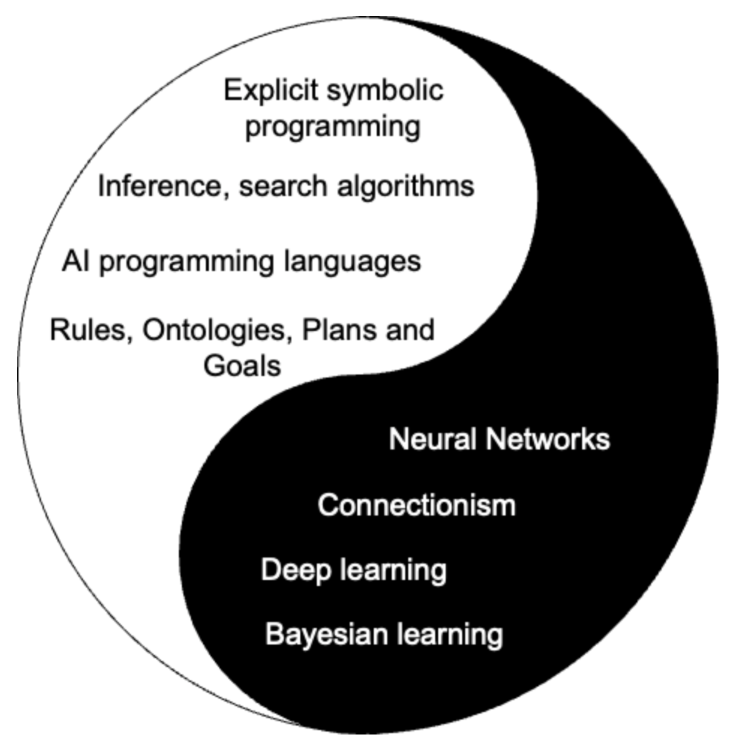
\includegraphics[width=.5\linewidth]{2_stateoftheart/figures/Lieberman_taxonomy.eps}
    \caption{AI Spectrum as depicted in \cite{lieberman_symbolic_nodate}}
    \label{fig:lieberman_tax}
\end{figure*}

Throughout the years, several categorizations have been proposed for the existing Artificial Intelligence (AI) models, each attending to a specific criterium. \cite{lieberman_symbolic_nodate} categorizes AI models considering their input in two categories: symbolic (also referred to as ``classic AI") and subsymbolic. These two types are disjoint and complimentary to each other. \cite{lieberman_symbolic_nodate} depicts the AI spectrum as a \textit{yin-yang} (Figure \ref{fig:lieberman_tax}), where the flaws of one kind are compensated by the benefits of the other. While this categorization presents a simple and general overview of the existing AI models, it lacks a middle ground where hybrid approaches can be categorized. 

Opposite to this vision, where the focus is on the input, \cite{loyola-gonzalez_black-box_2019} envisions the AI spectrum from the perspective of the output. This taxonomy categorizes AI approaches as \textit{white-box} or \textit{black-box} considering whether the process that lead to a given output can be explained or not. The notation \textit{black-box} is used to describe those models whose inference process cannot be explain, which mainly applies to machine learning models.  \textit{Black-box} models can be subsequently grouped in: hyperplane-based, neural networks, probability-based and instance-based. \textit{White-box} models lie on the opposite side of the spectrum, and relate to those approaches whose inference process can be understood and explained. Decision trees, rule-based systems, or fuzzy logic are encompassed in this category.


\begin{figure}
    \centering
    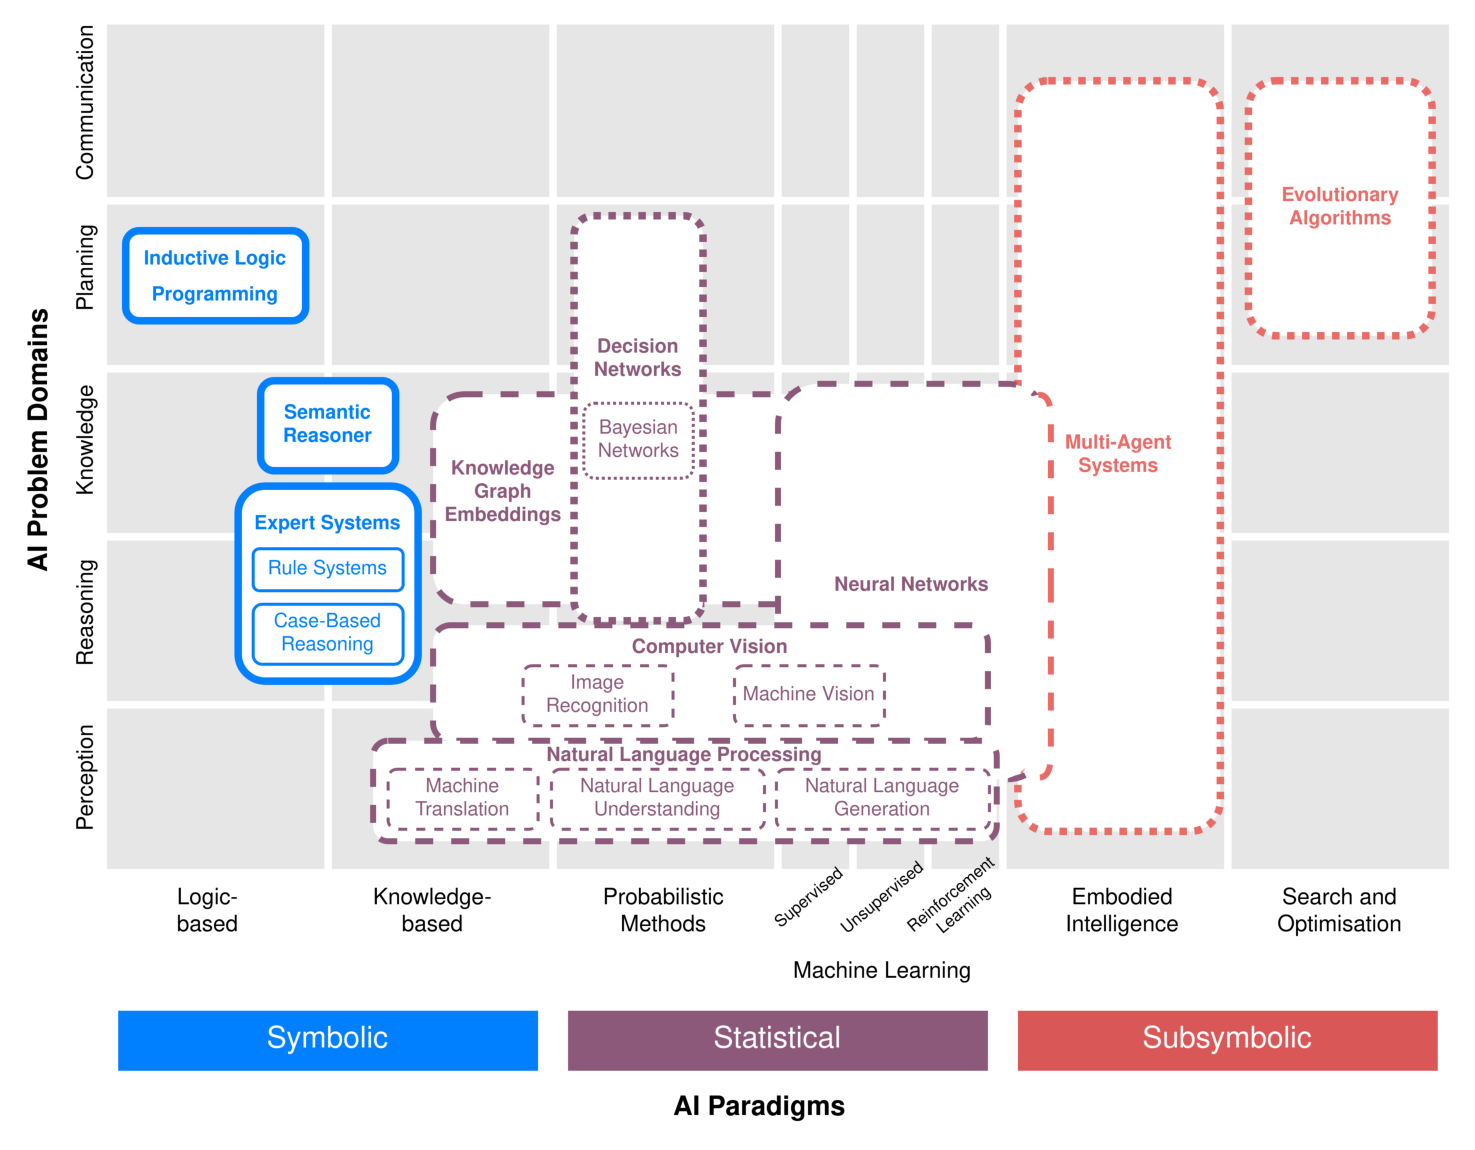
\includegraphics[width=\linewidth]{2_stateoftheart/figures/AI_Map.eps}
    \caption{Map of AI models combining the taxonomy of \cite{corea_ai_2019} with the taxonomy considered in this thesis. Symbolic, statistical and subsymbolic approaches are colour-coded in blue, purple and red respectively. Knowledge-based and computational intelligent systems are coded in continuous and non-continuous lines, respectively. Dashed lines depict deep learning approaches, while dotted lines depict other computational intelligent approaches.}
    \label{fig:ai_map}
\end{figure}


More recently, \cite{corea_ai_2019} proposed a two dimensional categorization of AI technologies. Instead of considering the input or output of the model, this taxonomy focuses on the application domains of each paradigm and its reasoning paradigm. Figure \ref{fig:ai_map} portrays this categorization, where the Y-axis comprises the existing problem domains, while the X-axis encodes the three considered paradigms: symbolic, statistical and subsymbolic. While the taxonomy proposed by \cite{lieberman_symbolic_nodate} only considered the symbolic (blue) and subsymbolic (red) categories, \cite{corea_ai_2019} also considers the statistical (purple) models as an in-between group between the two complimentary groups. Moreover, finer-grained subcategories can be distinguished inside each of the three main paradigms:
\begin{itemize}
    \item \textbf{Symbolic models:} The term \textit{symbolic} describes AI paradigms that not only employ symbolic representations as input, but have an inference process that can be understood and explained by humans. Two finer grained types are identified inside this category: logic-based and knowledge-based.
    \item \textbf{Statistical models:} While the taxonomy proposed by \cite{lieberman_symbolic_nodate} only comprised symbolic and subsymbolic models, which are treated as analogous and complimentary kinds, this taxonomy distinguishes statistical models from purely subsymbolic models. These models employ mathematical tools for reasoning and can be subsequently divided into probabilistic and machine learning models.
    \item\textbf{Subsymbolic models:} According to this taxonomy, the term \textit{subsymbolic} refers to the absence of previous knowledge needed to function. Embodied intelligence models and search and optimisation models are grouped under this criterion.
\end{itemize}

The previous taxonomies provided categories that were fully disjoint and, therefore, each particular model needed to belong to exclusively one of the types. The taxonomy of \cite{corea_ai_2019} enables a higher degree of flexibility, as models can be applied under different problem domains as well as use different reasoning paradigms.
%%Taxonomias de la mas antigua a la mas moderna
\cite{hopgood_2009_knowledge-based} proposed a division of AI paradigms in two main categories: knowledge-based systems and computationally intelligent systems. Knowledge-based systems require explicit representations of knowledge in a symbolic form, while computationally intelligent systems use nature-inspired paradigms where no background knowledge is required to reason. This taxonomy can be merged with the taxonomy of \cite{corea_ai_2019}, providing a three-dimensional taxonomy as depicted in Figure \ref{fig:ai_map}. A third dimension depicts whether the paradigm can be classified as knowledge-based (continuous line) or computationally intelligent (discontinuous line). 

Deep Learning was introduced after \cite{hopgood_2009_knowledge-based}'s taxonomy was defined and is therefore not featured in this categorization. Therefore, a slight update on this base taxonomy is proposed to include deep learning models. Figure \ref{fig:ai_map} makes a distinction inside the computationally intelligent models, denoting with a dashed instead of a dotted line those paradigms that can be considered as deep learning. 

After combining the taxonomies presented in \cite{hopgood_2009_knowledge-based} and \cite{corea_ai_2019}, the final three-dimensional categorization of the models is as follows:
\begin{itemize}
    \item \textbf{Knowledge-Based Systems:} These systems fit almost perfectly the definition previously provided for the symbolic paradigms. Therefore, this category groups all the models that require from background expert knowledge to reason:
    \begin{itemize}
        \item \textit{Inductive Logic Programming (ILP):} This term was first introduced by \cite{Muggleton1991}, describing this field as ``\textit{the area of AI which deals with the induction of hypothesised predicate definitions from examples and background knowledge}". ILP is one of the prime examples of symbolic learning, using fully expressive representations to encode logical clauses and knowledge, making the input, output and the induction process fully explainable.
        \item \textit{Semantic Reasoners:} Instead of expressing background knowledge by means of logical clauses or predicates as in ILP, semantic reasoners use ontologies to encode background knowledge. Ontologies \citep{noy2001ontology} provide explicit specifications of conceptualizations which are shared and understood between humans and machines. Moreover, ontologies present a formal definition of classes (or types) and the properties and relations between those classes and their instances in a given domain. From the information encoded in an ontology, a semantic reasoner (also referred to as the reasoning engine) can infer new axioms from the existing axioms.
        \item \textit{Expert Systems:} Formally, an expert system can be described as an AI system capable of emulating the decision-making process of a human expert of a given domain. These systems are composed by two differentiated parts: an inference engine and a knowledge base. The knowledge base encodes the facts, rules and background information needed. The inference engine applies the rules existing in the knowledge base to the known facts to infer new facts. \textit{Rule Systems} are the cornerstone of expert systems, using if-then clauses to infer new information from the already existing knowledge. As both facts and rules are encoded in a declarative way, the inference process can be fully understood and explained by humans. \elvitodo{A lo mejor esto hay que aumentarlo un poco}
        
        \textit{Case-Based Reasoning} (CBR) \citep{overview_cbr} is another example of an expert system. In this case, the knowledge base is replaced by a case base, where a set of problem-solution tuples (or cases) are stored. CBR implements a continuous cycle, where the model improves overtime by including the knowledge acquired from the resolution of new problems, whose solutions are then stored in the case base. Therefore, the performance of the model improves overtime. A CBR model is composed of four distinct phases: retrieve, reuse, revise and retain. When a new problem enters the system, the retrieve phase is triggered, returning the most similar existing cases to the introduced one. From the most similar cases, a tailored solution for the input problem is devised in the reuse stage using the already known solutions of the most similar cases. The proposed solution is then revised, determining whether it is suitable for the problem or not. If the solution satisfies the input problem, the newly generated case is stored in the case base, and will serve for the resolution of subsequent problems.   
    \end{itemize}
    \item \textbf{Computational Intelligence:} Following the taxonomy from \cite{hopgood_2009_knowledge-based}, computational intelligence models cover both statistical and subsymbolic paradigms. The remaining of the computational intelligence spectrum according to the proposed categorization comprises the following models:
    \begin{itemize}
        \item \textit{Decision Networks,} also referred to as influence diagrams \citep{poole_2017_ai_foundations} are graphical representations of a finite and sequential decision problem. A decision network is generally composed by three types of nodes: chance, decision and utility nodes, which are assorted as a directed cyclic graph. \textit{Bayesian Networks} \citep{friedman_1997_bayesian} are the most common paradigm amongst decision networks. Based on the Bayes theorem, these decision networks model the conditional dependencies between nodes, modelling the probability of each variable. Therefore, Bayesian networks can be used both to infer an outcome given the input variables as well as to determine the most feasible combination of variables that leads to an output. As variables are explicitly declared and their probabilities are known, the inference process of Bayesian networks can be also fully interpreted.
        \item \textit{Multi-Agent Systems} (MAS) \citep{Ferber:1999:MSI:520715} are one of the most extended paradigms for the simulation of scenarios involving complex entities. These models comprise a set of self-organized intelligent agents which cooperate and interact to perform a given task. As it involves several independent components, these models are capable of solving complex tasks that can not be solved by single-task systems. Agents of a MAS are autonomous, act locally, and are independent of each other. 
        \item \textit{Evolutionary Algorithms} \citep{GALVAN2003573} are heuristic-based systems inspired by natural evolution mechanisms. They are mostly applied to combinatorial problems, as they can greatly reduce the time required to go through the search space while still reaching an optimal solution. Typically, an evolutionary algorithm comprises four steps: initialization, selection, operation, and termination. These stages are closely related to those happening in natural selection. Therefore, those candidate solutions that better fit the problem will replicate and proliferate, while those inadequate will be slowly discarded throughout the evolution process. 
    \end{itemize}
    \item \textbf{Deep Learning} was first introduced in 2012 \citep{bengio_2012_dl_review}. This term was coined to describe the upcoming trend of computational intelligence models, especially neural networks, that are capable of reasoning at a very high level of abstraction. There is not a formal unified definition for the models encompassed in this trend, but they share common features such as requiring elevated computational resources, performing more than two in-between transformations between the input and the output (i.e: having more than two intermediate layers in neural networks) or learning multiple representations with different abstraction levels.
    \begin{itemize}
        \item \textit{Neural Networks}, are connected systems inspired by the neurological behaviour of brains \citep{Rosenblatt58theperceptron:}. These models are composed by the interconnection of single processing units called \textit{neurons}, capable of performing simple mathematical operations. A neural network receives an input, which is subsequently processed by the neurons to generate an output value. In order for the output value to be coherent with the input, the neural network requires a training (or learning) process, where the weights of the connections between the neurons are learned using the error gradient backpropagation from a loss function \citep{rumelhart_1987_backpropagation}.  
        
        % Three main types of neural network learning can be distinguished: supervised, unsupervised and reinforcement learning. In \textit{supervised learning}, a set of known inputs with their corresponding outputs 
        \item \textit{Computer Vision} is one of the primary fields of application of deep learning. This area encompasses methods capable of capturing, processing, analyze and reason over graphic data. Convolutional Neural Networks (or CNNs) have been the dominant paradigm of this area since 2012 \citep{alexnet}, reaching state-of-the-art results in most computer vision tasks.
        
        \item \textit{Natural Language Processing} (or NLP) \citep{chowdhury_2003_nlp} encompasses those models and tasks focusing on understanding, processing, and generating spoken and written words similarly to humans. While knowledge-based systems were previously predominant in the area, the existing models have been slowly replaced by a series of neural network architectures capable of performing the same tasks with remarkably better results. Some neural network architectures specific of this area include \textit{Bidirectional Long-Short Term Memories} (Bi-LSTM) \citep{devlin-etal-2019-bert,peters-etal-2018-deep} and \textit{Recurrent Neural Networks} (RNNs) \citep{wang-etal-2016-combination}. 
        
        \item \textit{Knowledge Graph Embeddings} \citep{dai_survey_2020} aim to arithmetically represent the information encoded in the facts contained in a knowledge graph, associating every entity and relation with a unique representation. The resulting depiction aims to embed the knowledge stored in the facts so that several constraints are met. One of the most important restrictions is that those entities representing similar concepts should have similar embeddings, meaning that the distance between their representations should be fairly small. According to the scoring function, two different types of approaches can be defined: translation-based and semantic matching models. Translation-based models aim to minimize distance-based scoring functions, while semantic matching models measure the plausibility of a given fact by matching the latent semantics of entities and relations.
    \end{itemize}

\end{itemize}

%%Nuestra taxonomia y cuales son cada uno 

% \section{Design Methods for Hybrid Learning Systems}
\section{Neurosymbolic Systems} \label{sec:sota_neurosymbolic_systems}
\textit{Neurosymbolic} (or hybrid learning) AI describes a set of proposed methods designed to integrate analogous AI models, generating new approaches that combine the benefits of both models under a unified framework. As \cite{valiant_three_2003} claimed: ``\textit{The aim is to identify a way of looking at and manipulating commonsense knowledge that is consistent with and can support what we consider to be the two most fundamental aspects of intelligent cognitive behaviour: the ability to learn from experience and the ability to reason from what has been learned"}. Several efforts have been conducted on this direction, proposing strategies, categorizations, and studying the limitations of this integration. 

\subsection{Motivation}\label{2_sec:subsec:motivation}
%%Papers referentes a por qué, limitaciones, etc. Aquí va el paper de sensors
\cite{mcgarry_hybrid_1999} theorized about the potential benefits of combining symbolic and subsymbolic systems, represented by rule-based systems and neural networks, respectively. According to \cite{mcgarry_hybrid_1999}: ``\textit{The ability of neural networks to perform tasks that would otherwise prove difficult or intractable to symbolic computing systems is now recognized}". This statement illustrates the main claim behind neurosymbolic systems: combining the benefits of symbolic and subsymbolic models such that the resulting hybrid system enables the solution of tasks that can not be solved by just one of the kinds. 

% This statement has been subsequently validated by various works throughout the years, such as \cite{mira_neurosymbolic_2004}, \cite{bader_dimensions_2005} or \cite{garcez_neural-symbolic_2019}.

\begin{table}
\centering
\caption{Application domain and assessment of the works employing predictive techniques over knowledge bases. 
%Define if appropriate
The metrics reported in the table are: M1 (scalability), M2 (interpretability), M3 (generalization capability), M4 (low resource consumption) and M5 (knowledge base exploitation). The degree of fulfilment of each metric per resource is indicated as follows:$\times$ = yes/high, / = partly/medium, empty = no/low. Symbolic and subsymbolic approaches are depicted in green and red respectively. \label{tab:sensors_reasoning}}
\resizebox{.75\linewidth}{!}{
%\begin{tabular}{C{3.5cm}C{2.5cm}C{3.5cm}C{2.5cm}C{2.5cm}C{1cm}C{1cm}C{1cm}C{1cm}}
\begin{tabular}{M{3.5cm}M{2.2cm}M{4cm}M{.5cm}M{.5cm}M{.5cm}M{.5cm}M{.5cm}M{1.5cm}}
\toprule
{\textbf{Resource}} &
{\textbf{Domain}} &
\textbf{Predictive} \textbf{Technique} &
{\textbf{M1}} &
{\textbf{M2}} &
\textbf{M3} &
\textbf{M4} &
\textbf{M5} &
\textbf{Score} \\
\midrule
\rowcolor{teagreen}\cite{aliandlee}         & \textit{Health}                   & \textit{Rules Manually Created by Experts}                           &                      &$\times$                         &                                 &$\times$                                 &$\times$                        & 3                      \\
\rowcolor{teagreen}\cite{barnwaletal}      & \textit{Risk/Resource Management} & \textit{Probabilistic distributions}                                 &                      &$\times$                         &                                 &$\times$                                 &$\times$                        & 3                      \\ 
\rowcolor{tearose}\cite{bogaleetal}       & \textit{Multidomain}              & \textit{Multivariate Linear Regression}                              & /                    & /                         & /                               &$\times$                                 &$\times$                        & 3.5                    \\ 
\rowcolor{tearose}\cite{chungetal2018}        & \textit{Health}                   & \textit{Deep Neural Network}                                         &$\times$                    &                           &$\times$                               &                                   &$\times$                        & 3                      \\
\rowcolor{tearose}\cite{dimitrovetal}     & \textit{Housing}                  & \textit{Bayesian Network} \citep{bayesiannetwork}                                             &                      &$\times$                         &                                 &$\times$                                 &$\times$                        & 3                      \\ 
\rowcolor{teagreen}\cite{duyenandnhon}      & \textit{Education}                & \textit{If-then manually created rules}                              &                      &$\times$                         &                                 &$\times$                                 &$\times$                        & 3                      \\ 
\rowcolor{tearose}\cite{fastetal}         & \textit{Housing}                  & \textit{Word2Vec vector generation + cosine distance comparison}     &$\times$                    &$\times$                         &$\times$                               & /                                 &$\times$                        & 4.5                    \\ 
\rowcolor{tearose}\cite{haoetal}          & \textit{Housing}                  & \textit{Half-Duplex Search algorithm}                                &                      &$\times$                         &                                 &$\times$                                 &$\times$                        & 3                      \\ 
\rowcolor{tearose}\cite{kimandchung}       & \textit{Health}                   & \textit{Neural Network}                                              &$\times$                    &                           &$\times$                               & /                                 &                          & 2.5                    \\ 
\rowcolor{teagreen}\cite{KimandChang}       & \textit{Health}                   & \textit{Pearson's correlation coefficient + Collaborative Filtering} \citep{pearsoncorrelation,collaborativefiltering,collaborativefiltering2} &                      &$\times$                         &                                 &$\times$                                 &$\times$                        & 3                      \\ 
\rowcolor{tearose}\cite{machadoetal}      & \textit{Housing}                  & \textit{Multi-entity Bayesian Networks} \citep{mebn}                              &                      &$\times$                         &                                 & /                                 &$\times$                        & 2.5                    \\ 
\rowcolor{teagreen}\cite{Martinruizetal}  & \textit{Health}                   & \textit{Rules manually created by experts}                           &                      &$\times$                         &                                 &$\times$                                 &$\times$                        & 3                      \\ 
\rowcolor{teagreen}\cite{olszewskiturek} & \textit{Mobility}                 & \textit{CART Trees} \citep{carttrees}                                                   & /                    &$\times$                         &$\times$                               &$\times$                                 &$\times$                        & 4.5                    \\
\rowcolor{teagreen}\cite{Olzewskietal}    & \textit{Government}               & \textit{Fuzzy logical rules} \citep{fuzzyenvironment}                                         &                      &$\times$                         & /                               &$\times$                                 &$\times$                        & 3.5                    \\ 
\rowcolor{teagreen}\cite{orlowskietal}     & \textit{Mobility}                 & \textit{Fuzzy logical rules}                                         &                      &$\times$                         & /                               &$\times$                                 &$\times$                        & 3.5                    \\ 
\rowcolor{teagreen}\cite{peraletal}        & \textit{Health}                   & \textit{C4.5 Tree} \citep{c45tree}                                                   &                      &$\times$                         &                                 &$\times$                                 & /                        & 2.5                    \\ 
\rowcolor{tearose}\cite{persaudetal}      & \textit{Mobility}                 & \textit{Deep Neural Network}                                         &$\times$                    &                           &$\times$                               &                                   & /                        & 2.5                    \\ 
\rowcolor{tearose}\cite{ribonietal}       & \textit{Health}                   & \textit{Random Forest} \citep{randomforest}                                               &$\times$                    & /                         &$\times$                               & /                                 &$\times$                        & 4                      \\ 
\rowcolor{tearose}\cite{siimobility-parking,siimobility-consult,siimobility-journal}        & \textit{Mobility}                 & \textit{Bayesian Regression ANNs} \citep{brann1,brann2,brann3}                                     &$\times$                    & /                         &$\times$                               & /                                 &$\times$                        & 4                      \\
\rowcolor{teagreen}\cite{xuandli}           & \textit{Risk/Resource Management} & \textit{Fuzzy logical rules}                                         &                      &$\times$                         & /                               &$\times$                                 &$\times$                        & 3.5                    \\ 
\rowcolor{teagreen}\cite{zavalaetal}       & \textit{Mobility}                 & \textit{RIPPER rules} \citep{ripper}                                                &                      &$\times$                         &                                 &$\times$                                 &$\times$                        & 3                      \\ \bottomrule

\end{tabular}
}
\end{table}
A systematic review was conducted in the context of ambient intelligence to further explore the existence, limitations, and causes of the application of neurosymbolic models. This work is extensively presented in \cite{amador_systematic_review_2019}\footnote{Elvira Amador-Domínguez, Emilio Serrano, Daniel Manrique, & Juan F. De Paz (2019). Prediction and Decision-Making in Intelligent Environments Supported by Knowledge Graphs, A Systematic Review. Sensors, 19(8), 1774. doi:10.3390/s19081774}, being one of the contributions of this thesis. The conducted review studies the interactions between knowledge bases (KBs) and machine learning models, as well as their specific applications. Different application subdomains were identified to clearly identify the scope of application of each proposal. This finer-grained analysis enables a better comprehension of the reasons why a certain model is chosen for a certain task. The identified subdomains, following the categorization proposed by \cite{ahmedetal} are: health, housing, education, mobility, risk and resource management, government, and multidomain. Another main goal of this study is to assess whether and how background knowledge (in the form of a knowledge base) is integrated into different predictive and decision-making models.

Background knowledge was mostly extracted from three sources: data provided by users, previously existing KBs, and sensor data, being the latest the most prominent one. Regarding the role of the KB, it varies greatly across the different subdomains. In the health, mobility, risk and resource management and housing domains, the KB is built with the purpose of subsequently feeding a predictive model, doting it with background knowledge and enhancing its reasoning capabilities. This statement does not hold in the government and education domains, where the KB plays the primary role instead of serving as a secondary element.

The following metrics (which relate to the expected features of neurosymbolic systems) were evaluated to study the different proposals in which the KB is integrated within the predictive model: scalability, interpretability, generalization ability, resource consumption, and relevance of the knowledge base to the predicting process. Table \ref{tab:sensors_reasoning} summarizes the findings of this study. Despite the heterogeneity between proposals, it is worth noticing that the majority of the employed paradigms are symbolic (green highlighted rows), thus scoring high in interpretability (M2). In the work of \cite{olszewskiturek} a neural network is also evaluated on the task, outperforming other approaches. The authors, however, decide on a decision tree as their final model, stating that even when its performance was subpar with respect to the neural network, they preferred to employ a model that was interpretable. This decision is quite remarkable, as it clearly showcases one of the biggest breaches between symbolic and subsymbolic models: the lack of explainability. 

All proposals used the KB when building the predictive model, thus successfully integrating background knowledge. It is also worth noticing that, for subsymbolic approaches (red coloured rows), there exists a direct relation between scalability (M1) and generalization capability (M3), featuring simultaneously on several resources. This does not apply to purely symbolic models, where these features are ranked either as partial or null. This study served to further evidence the existing chasm between symbolic and subsymbolic approaches, evidencing the necessity of middle-ground solutions that combine the positive features of both types.

%Después de nuestra referencia, el resto

\subsection{Design}\label{2_sec:subsec:design}
%Papers de boxología
\cite{mcgarry_hybrid_1999} is one of the first works to draw the limitations of neurosymbolic models, focusing on the integration of neural networks and rule-based systems. According to this work, the key features a neurosymbolic system should present are: i) the ability to reason with noisy and incomplete data, ii) learning incrementally from new experience, iii) generalize and explain the chain of reasoning. %%LUEGO ESTO SE EXTIENDE

\begin{figure}
    \centering
    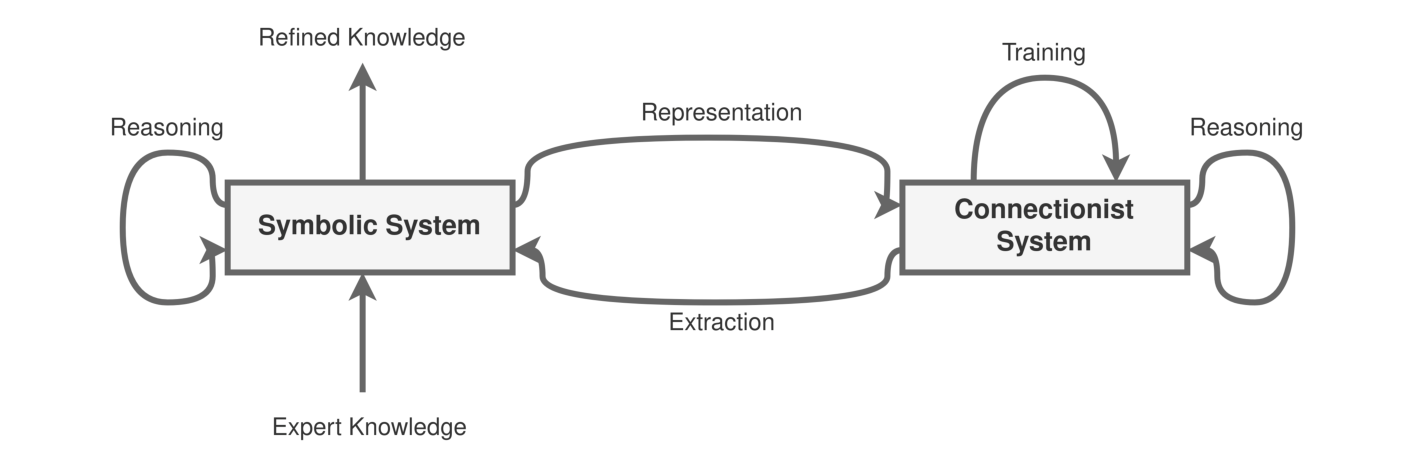
\includegraphics[width=\linewidth]{2_stateoftheart/figures/Neurosymbolic_Bader.eps}
    \caption{Neurosymbolic learning cycle. Extracted from \cite{bader_dimensions_2005}}
    \label{fig:neuro_cycle}
\end{figure}

This idea was further expanded by \cite{bader_dimensions_2005}, which introduced neurosymbolic learning as a continuous cycle. Figure \ref{fig:neuro_cycle} illustrates this idea, where interactions between the symbolic and subsymbolic systems do not occur in a linear way, but in a close cycle composed by individual interactions between both. For example, the symbolic system could play the role of a front-end, where expert knowledge is collected. This knowledge could then be encoded into the subsymbolic system during the training process, providing additional information that may not be inferred otherwise by the model. Moreover, the knowledge acquired throughout the training process could be extracted, decoded, and introduced back to the symbolic system, introducing new patterns of restrictions that may not have been previously declared. This cyclical conception of neurosymbolic systems meets the features proposed by \cite{mcgarry_hybrid_1999}.

\cite{mira_neurosymbolic_2004} roots the creation of neurosymbolic models on two criteria: purpose and design. For the first criterion, the authors determine that neurosymbolic integration is required in those scenarios where neither all knowledge or data are available. Regarding the design of the system, two strategies are proposed:
\begin{itemize}
    \item \textit{Unification}, where the needs of both symbolic and subsymbolic models are merged into a single component. This design induces a certain level of explainability to the connectionist models, while still retraining their topology and learning capabilities.
    
    % Two different design paths are proposed for this: i) extending the computational capabilities of the connectionist models to include symbolic forms of representation and ii) reducing the grain size of the symbolic model to enable subsymbolic representation. These two paths converge to the replacement of connectionist local functions by parametric rules. 
    \item \textit{Hybridation}, where the symbolic and connectionist modules are interconnected. In this design, connectionist components serve as a supporting element to the main symbolic processor.
\end{itemize}

With the renewed interest in neurosymbolic computing, new proposals have emerged addressing the newly existing challenges in neurosymbolic computing. \cite{besold_neural-symbolic_2017} enunciated a set of principles for neurosymbolic integration. This work highlights one of the core elements of neurosymbolic models: the distinction between representation and reasoning. Typically, symbolic models play the representation role, while subsymbolic models are used for reasoning. Equal to \cite{bader_dimensions_2005}, \cite{besold_neural-symbolic_2017} envisions neurosymbolic integration like a cycle, comprising the following steps: i) translation of symbolic background knowledge to a subsymbolic representation, ii) training the subsymbolic model to extract general patterns about the data, iii) reason over new data using the subsymbolic model and iv) extract symbolic knowledge from the subsymbolic model. The final step not only provides explanation of the inference process, but facilitates transfer learning over the subsymbolic model.

\begin{figure}[h]
    \centering
    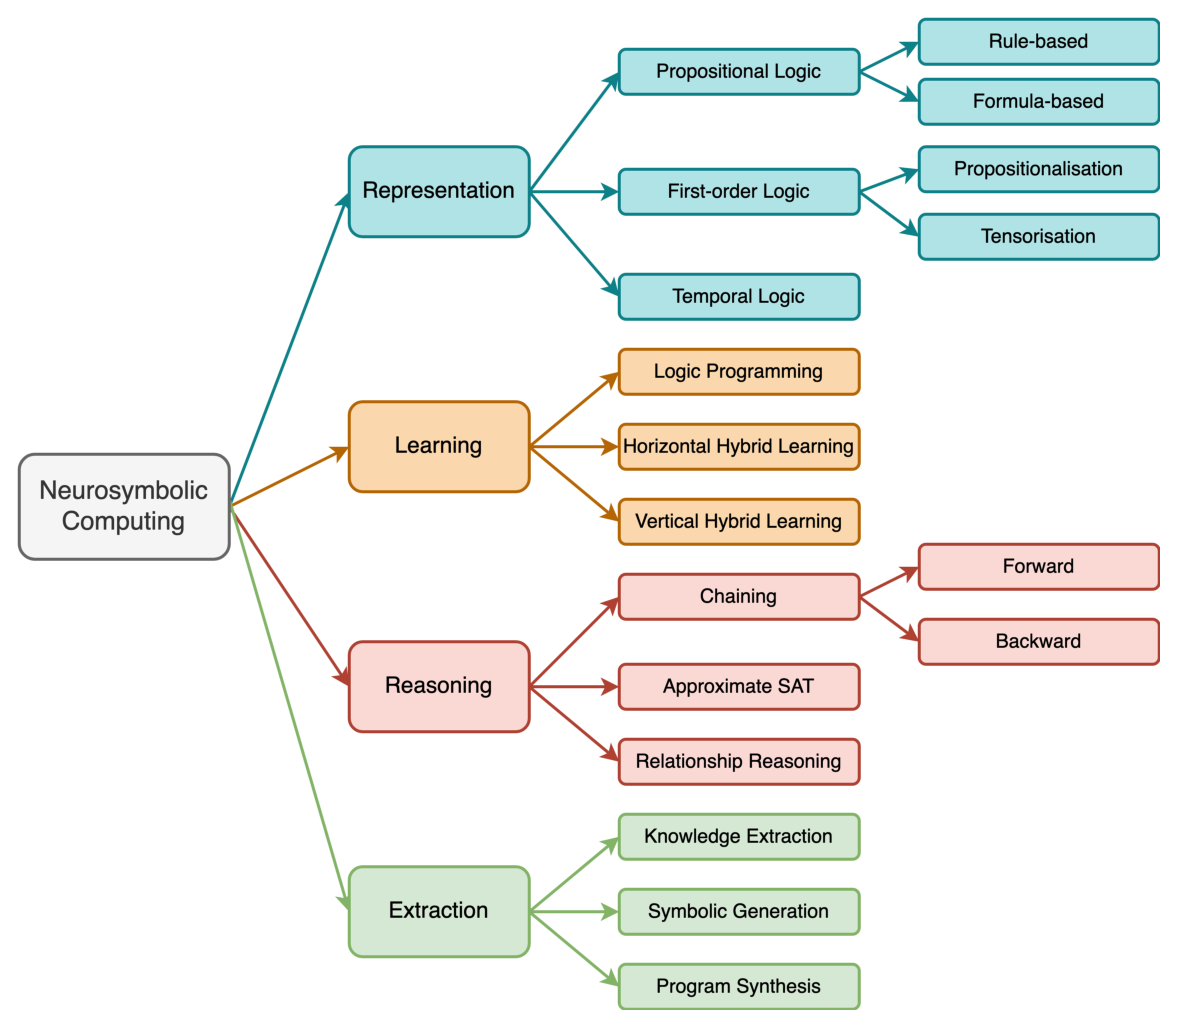
\includegraphics[width=.9\linewidth]{2_stateoftheart/figures/garcez_design.eps}
    \caption{Design dimensions proposed by \cite{garcez_neural-symbolic_2019}}
    \label{fig:garcez_design}
\end{figure}

\cite{garcez_neural-symbolic_2019} proposed a methodology for neurosymbolic integration that focuses on four key features: representation, extraction, reasoning, and learning. Figure \ref{fig:garcez_design} depicts the different design dimensions per feature. This methodology is compatible with the cyclic neurosymbolic learning process depicted in \cite{bader_dimensions_2005} and \cite{besold_neural-symbolic_2017}, but addresses additional features that were not previously considered and that are key to define neurosymbolic models.

\cite{garcez_neurosymbolic_2020} state that there always exist at least two options for designing a neurosymbolic model. In the first option, symbolic representations are translated and fed into a connectionist system, using the connectionist system to perform reasoning. In the second option, both the symbolic and connectionist models interact to perform reasoning. \elvitodo{Ampliar(?)}


%Regarding representation, \cite{garcez_neural-symbolic_2019} distinguishes three main groups: rule-based, formula-based, and embedding-based. In rule-based representation, the goal is to tailor the design of the connectionist system to mimic the representation of a rule system. Formula-based representations focus on mapping logical formulas to connectionist models. Finally, embedding-based representation projects symbolic representations into a continuous vector space, such that they can serve as input for a connectionist model. 

Some works focus on the visual representation of neurosymbolic systems via design patterns. \cite{harmelen_boxology_2019} introduces a boxology of design patterns for neurosymbolic systems. This work introduces a simple notation, composed by two types of representation techniques (data and symbolic) and two types of reasoning models (knowledge-reasoning and machine learning). This notation, while simple, is enough to represent any neurosymbolic system from a high-level perspective. \cite{van_bekkum_modular_2021} proposed an extension of this representation, providing a collection of compositional patterns with a higher specificity degree. This design methodology extends the two existing elements in the previous taxonomy with two additional types: processes and actors. In this design, \textit{processes} are used to describe operations that are performed outside the reasoning model, such as data transformation or instance generation. \textit{Actors} describe those autonomous elements that are external to the model but actively interact with the neurosymbolic system, such as humans, external apps or sensors.

%%Modelos hibridos, por que se reemplazan unos a otros, beneficios, aproximaciones, clasificaciones dentro de este marco. 

\subsection{Categorization}\label{2_sec:subsec:categorization}
The neurosymbolic classification framework proposed by \cite{medsker2020models} is one of the first efforts of categorizing neurosymbolic hybrid models under a unified framework. Five integration strategies are defined from a practical point of view based on the interaction degree, from fully independent to fully integrated: stand-alone, transformational, loose coupling, tight coupling, and fully integrated. This categorization does not model the input and output representations employed by each category, as well as the order in which the symbolic and connectionist modules are arranged.


\cite{hilario_overview_nodate} proposed a finer-grained categorization for neurosymbolic models. This work posed a distinction between the two main strategies of neurosymbolic integration: unification and hybridation. Unified systems are built on the idea that symbolic structures and processes are not strictly required and can emerge from their neural counterparts. On the contrary, hybrid systems are based on the synergistic combination of neural and symbolic models, leading to systems with enhanced cognitive and computational capabilities. Amongst the unified systems, \cite{hilario_overview_nodate} distinguishes between \textit{neuronal symbol processing} (NSP) and \textit{connectionist symbol processing} (CSP). While NSP aims to model the brain's high level functions emulating the behaviour of a real biological neuron, CSP is built for a specific task, commonly using artificial neural networks. Regarding hybrid strategies, they can be further categorized in functional and translational. Translational hybrids serve as a bridging element between unified models and functional hybrids, using symbolic structures with connectionist processors, but removing the need for a symbolic processor. Functional hybrids comprise complete symbolic and connectionist elements, combining neural networks with both symbolic structures and their processing elements. They can further be divided into loose and tight according to the degree of coupling between the symbolic and connectionist processors. 

%\begin{figure}
%    \centering
%    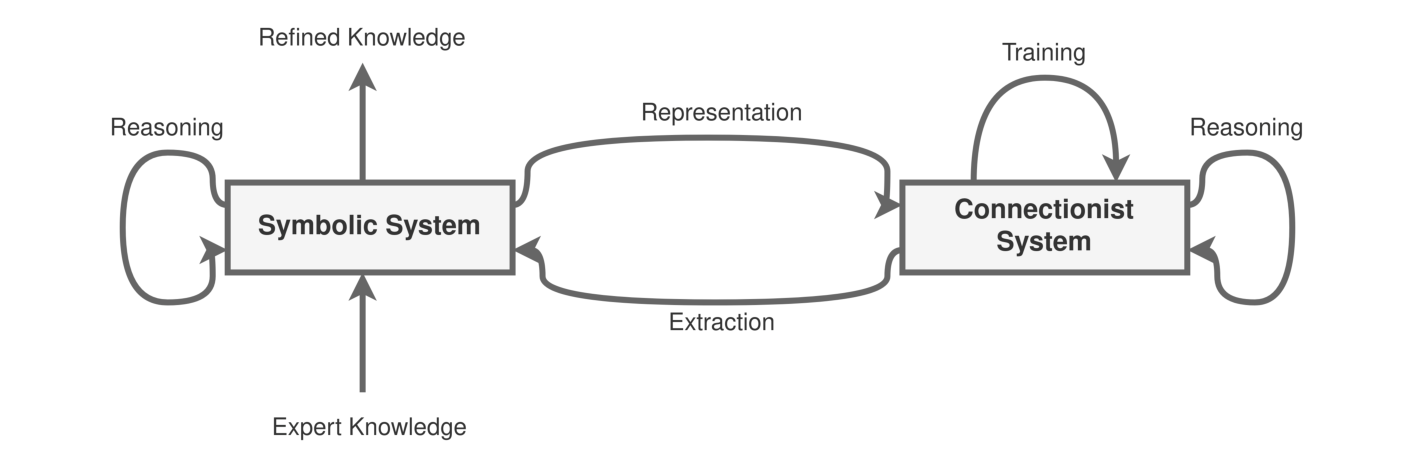
\includegraphics[width=\linewidth]{2_stateoftheart/figures/Neurosymbolic_Bader.eps}
%    \caption{Neural-symbolic learning cycle. Extracted from \cite{bader_dimensions_2005}}
%    \label{fig:bader_neurosymbolic}
%\end{figure}

\cite{mcgarry_hybrid_1999} focused on the categorization of a specific type of neurosymbolic models comprised by neural networks and rule-based systems. This categorization describes three integration types: \begin{itemize}
    \item \textit{Unified systems} implement a symbolic reasoning processing using subsymbolic elements, motivated by the idea that certain types of rule-based inference can be performed by subsymbolic models. The main limitation of these systems is their lack of scalability, as they rely on a symbolic-like representation paradigm.
    \item \textit{Translational systems} transform an initial symbolic representation into a subsymbolic one and viceversa. This bidirectional transformation enables, for example, the extraction of rules from neural networks, as well as the introduction of explicit background knowledge into the network. 
    \item \textit{Modular systems} are the most common type, integrating different individual modules (both symbolic and subsymbolic) under a unified framework.
\end{itemize} 

The categorization by \cite{hilario_overview_nodate} was later updated by \cite{bader_dimensions_2005}, proposing a more robust schema comprising three different dimensions. Instead of considering neurosymbolic integration as linear phenomena, \cite{bader_dimensions_2005} consider this process as a cycle. In this cycle, the symbolic system serves as an input point where expert knowledge can be collected, to be then fed into a connectionist system that can benefit from this background knowledge during the training process. Similarly, the knowledge acquired by the connectionist system after training can be returned to the symbolic system for further usage.

This conception of neurosymbolic integration enables a higher degree of flexibility than the previous categorizations. Subsequently, the categorization proposed by \cite{bader_dimensions_2005} provides a three-dimensional space, where each dimension has different degrees of flexibility. The categorization proposed in \cite{hilario_overview_nodate}, where models range from unified to translational, is treated as just one dimension in this categorization. This dimension is referred to as \textit{interrelation} in this categorization. The second dimension refers to the \textit{language}, which relates to the way in which the knowledge is encoded in the system. The third and final dimension encodes the \textit{usage} of the system.

%%Patrones de diseño con boxologia
\section{Introductory Integration of Deep Learning and Knowledge-Based Systems}  \label{sec:sota_dl_kb_intregration}

As discussed in the previous Section, several strategies can be followed regarding neurosymbolic system design. All these strategies, however, can be grouped in two main trends: introduction and extraction. Introductions approaches aim to combine symbolic and subsymbolic models under a unified framework to perform a certain task. In \cite{van_bekkum_modular_2021} several compositional integrative patterns are described, covering an extended set of tasks. 

Rules and deep learning models is one of the most recurrent combinations in neurosymbolic systems. \cite{hatzilygeroudis_integrated_2010} proposed the concept of the \textit{neurules}, a kind of integrated rules composed by several adaline units. \textit{Neurules} are also capable of successfully integrating external inputs and providing a better generalization. More recently, \cite{daniele_knowledge_2019} proposed Knowledge Enhanced Neural Networks, a neural architecture where prior knowledge is injected in the form of logical clauses. The introduction of rules in the network prevents it from learning contradictory patterns from the training data, making the final system robust to noisy data. This idea is further explored by \cite{roychowdhury_regularizing_2021}, where an architecture-agnostic method is proposed to integrate first-order logic clauses into deep learning models. The inclusion of first-order logic clauses successfully reduces the need of training data required, while simultaneously boosting the final performance of the system. \cite{kursuncu_knowledge_2020} studied a different path, proposing an architecture where knowledge graphs and expert knowledge are integrated within the learning process, alongside with external data. This integration not only enhances the results of the system, but also accelerates its convergence.

\begin{figure}[t!]
    \centering
    \subfigure[Knowledge Graph Embedding \label{fig:van_bekkum_kgc_kge}]{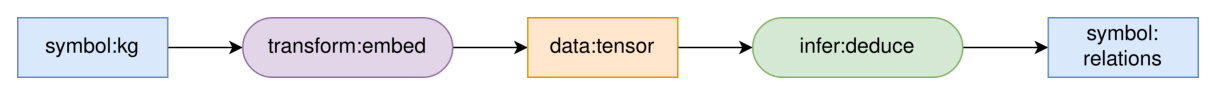
\includegraphics[width=.9\columnwidth]{2_stateoftheart/figures/vanBekkum_LinkPrediction.eps}}
    \subfigure[Graph Neural Network \label{fig:van_bekkum_kgc_gnn}]{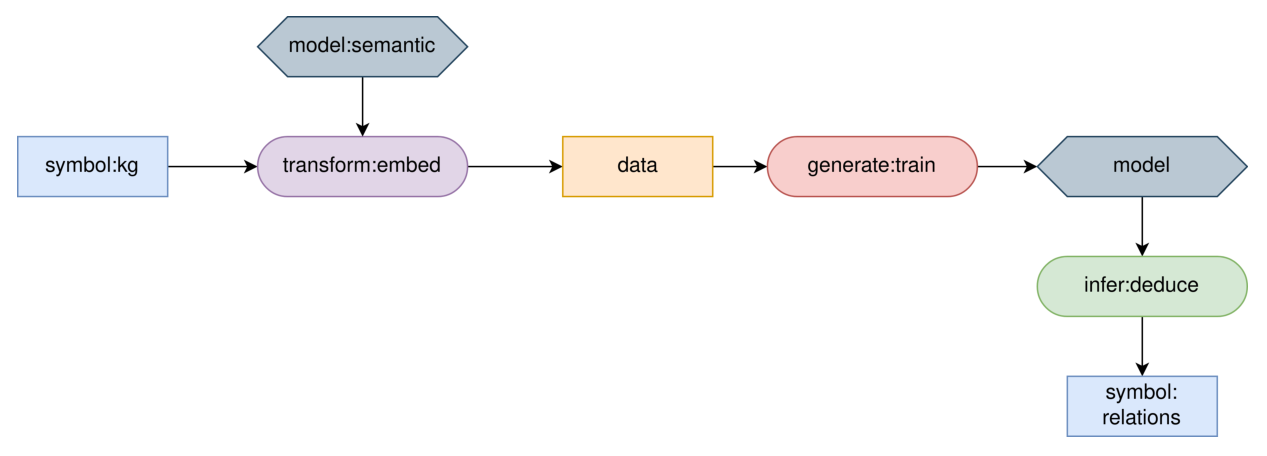
\includegraphics[width=.9\columnwidth]{2_stateoftheart/figures/vanBekkum_GNN.eps}}
    \caption{Design pattern of two Knowledge Graph Completion models according to \cite{van_bekkum_modular_2021}}
    \label{fig:van_bekkum_kgc}
\end{figure}

Knowledge Graph Completion \citep{nickel_review_ml_kg_2016,wang_kge_survey_2017} is one of the main scenarios of neurosymbolic integration. Knowledge Graphs are composed by three elements: a set of entities $\mathcal{E}$, a set of relations $\mathcal{R}$, and the interactions between entities and relations, denoted as \textit{facts} or triples. Facts follow the fixed structure $(s,p,o)$, where $s$ and $o$ are the \textit{subject} and \textit{object} entities respectively, and $p$ is the \textit{predicate} that connects them. KGC aims to mine new facts from the existing KG information. Two main subtasks can be identified within KGC: link prediction and triple classification. In triple classification, the goal is to determine whether a potential fact $(s',p',o')$ is feasible or not. In link prediction, given an incomplete fact $(?,p,o)$ or $(s,p,?)$, the goal is to find the remaining element that maximizes the feasibility of the fact. 

Figure \ref{fig:van_bekkum_kgc} depicts the design patterns (according to \cite{van_bekkum_modular_2021}) of the two main approaches for KGC. Figure \ref{fig:van_bekkum_kgc_kge} depicts the general pattern of a Knowledge Graph Embedding model for KGC. These neurosymbolic models follow a straightforward approach, where the symbolic input (KG) is converted into a tensor representation with an embedding operation. This subsymbolic representation can be used to infer new facts, which can be then decoded back to a symbolic format. Graph Neural Networks (Figure \ref{fig:van_bekkum_kgc_gnn}) can also be used for this purpose. These models require the integration of background semantic knowledge to embed the input KG into a vectorial space. The resulting representations can be used to train a neural network, which are used to deduce new facts.

\cite{leake_bringing_2020} studied the integration of case-based reasoning methodology with deep learning techniques. Case-based reasoning (CBR) is often perceived as an alternative to rule-based systems, the predominant symbolic paradigm of neurosymbolic systems. This integration is motivated by three key challenges existing in deep learning models: i) learning with fewer labeled samples, ii) learning to reason, and iii) learning to plan complex action sequences. These issues have been successfully addressed by case-based reasoning models, thus motivating the integration of both paradigms. Such is the case of the work by \cite{marie_segmentation_2019}, where a CBR model is combined with a Convolutional Neural Network to segment medical images. This proposal presents CBR as a solution to quality data insufficiency, serving as a preprocessing and augmentation mechanism for the network. \cite{lamy_explainable_2019} studied the possibility of exploiting CBR models' interpretability to explain the predictions of a deep neural network.


% \section{Deep Learning Enhanced Knowledge-Based Systems}
% %%Ejemplos de esto. Extraemos limitaciones y cositas y criterios.

%%\section{Knowledge Integration for Deep Learning Models} \label{sec:kb_dl_extraction_rw}

% %%Same

%%Extraido from neurosymbolic AI 3rd wave
%%%Despite the impressive results, deep learning has been criticised for brittleness (being susceptible to adversarial attacks), lack of explainability (not having a formally defined computational semantics or even intuitive explanation, leading to questions around the trustworthiness of AI systems), and lack of parsimony (requiring far too much data, computational power at training time or unacceptable levels of energy consumption)

\section{Knowledge Extraction from Deep Learning Models} \label{sec:sota_knowledge_extraction_dl}
% %%Same same
Opposite to integration, extraction describes hybrid approaches where one of the models is used to mine specific knowledge from the other. This is well exemplified in ontology learning \citep{Bouraoui_Jameel_Schockaert_2017,wong_ontology_2012,asim_ontology_2018}. Figure \ref{fig:van_bekkum_onto_learning} depicts the general ontology learning process, where one model is trained to predict a set of relations from a text guided by an auxiliary statistical model. The set of mined relations serves as the input for a second model, which generates a taxonomy from the input relations with the assistance of an external semantic model. 

\begin{figure}[t!]
    \centering
    \subfigure[Ontology Learning \label{fig:van_bekkum_onto_learning}]{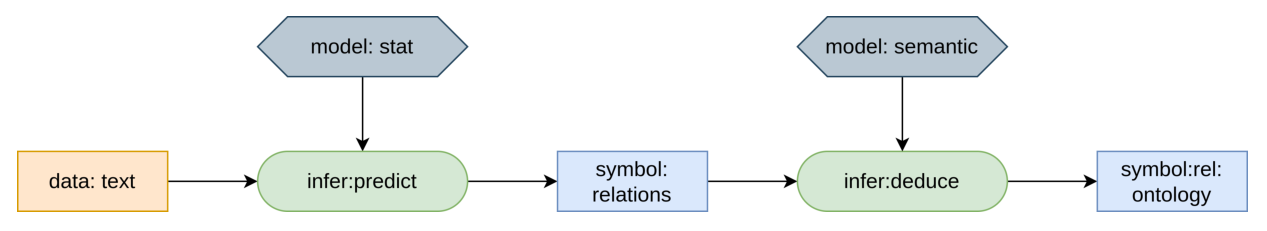
\includegraphics[width=.9\columnwidth]{2_stateoftheart/figures/VanBekkum_OntologyLearning.eps}}
    \subfigure[Instance-based Explaination \label{fig:van_bekkum_explain}]{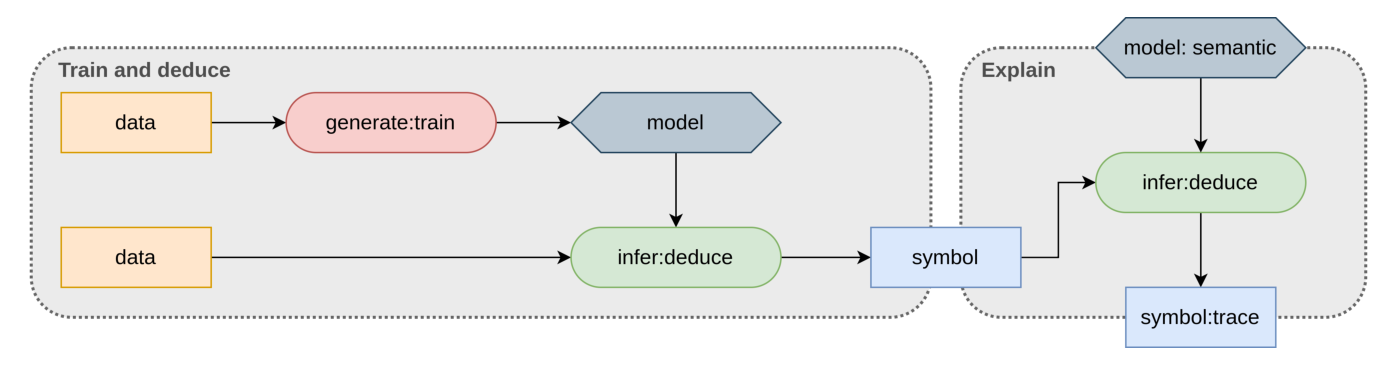
\includegraphics[width=.9\columnwidth]{2_stateoftheart/figures/VanBekkum_Explainability.eps}}
    \caption{Design pattern of two knowledge extraction models according to \cite{van_bekkum_modular_2021}}
    \label{fig:van_bekkum_explain_complete}
\end{figure}

Explainable Artificial Intelligence (XAI) is the main area of application of these approaches. As stated in \cite{angelov_explainable_2021}: ``\textit{As Artificial Intelligence and Machine Learning (and, especially, Deep Learning) become more wide spread and intertwined with human-centric applications, and algorithmic decisions become more consequential to individuals and society, attention has shifted back from accuracy to explainability"}. This is further evidenced by the results obtained in \cite{amador_systematic_review_2019}, where explainable methods were widely favoured as opposite to more accurate but opaque ones. \cite{burkart_survey_2021} provides a set of reasons why AI models should be explainable, namely: \textit{trust, causality, transferability, informativeness, fair and ethical decision making, accountability, adjustment-making} and \textit{proxy functionality}. These features are not inherent to deep learning models, and should therefore be enforced.

While \textit{explainability} is the general term used to describe these approaches, a variety of different terms are employed in the literature. Amongst the existing terms, the following are the most prominent ones, each presenting a different nuance \citep{barredo_arrieta_explainable_2020,adadi_explainability_2018,gilpin_explainability_2018}:
\begin{itemize}
    \item \textit{Transparency} refers to the capacity of a model to be fully understandable by itself.
    \item \textit{Interpretability} describes the capacity to provide an interpretation of the inference process that can be understandable by humans. 
    \item \textit{Explainability} is associated with the idea of explainations serving as an interface between humans and the AI system, which must be accurate and comprehensible by humans \citep{guidotti_explainability_2018}.
    \item \textit{Understandability} relates to the quality of a model to be human-understandable by design, without the need of explaining its internal processes.
    \item \textit{Comprehensibility} denotes the ability of a model to represent its learning process in a human-understandable manner.
\end{itemize}

More recently, \cite{phillips_explainability_2021} outlined the \textit{four principles of XAI}, defining the fundamental principles required by an AI system to be considered explainable:

\begin{itemize}
    \item \textit{Explaination:} The system must supply evidence or reasoning for each decision made by the system.
    \item \textit{Meaningfulness:} Explanations provided by the system must be meaningful and understandable by its users.
    \item \textit{Accuracy:} The explanation provided by the AI system must be an accurate reflection of the system's behaviour.
    \item \textit{Knowledge Limits:} Cases where the system can not operate must be identified, as their explanations may be misleading of the behavior of the system.
    
\end{itemize}

%%Explainable AI
Figure \ref{fig:van_bekkum_explain} gives an overview of a general explainability workflow. Two stages can be clearly differentiated in the process: training and deduction phase and explaining phase. The example showcased in Figure \ref{fig:van_bekkum_explain} describes an instance-based explaination model. LIME \citep{ribeiro_lime_2016} and Anchors \citep{Ribeiro_Singh_Guestrin_2018} are examples of such approaches, where the inference process of a single prediction made by a supervised classifier is explained by means of the predictions achieved by a sample of similar inputs. These approaches serve as a cornerstone for newer, more robust, and complex explainability frameworks, such as \cite{arya_one_2019}. 

While most explainability approaches focus on explaining neural network predictions, this trend is further expanded to different areas, such as KGC. Bianchi et al. \citep{bianchi_kge_explainability_2020} provided an study about explainability in KGE models. In the context of knowledge graph embeddings, explainability encompasses any potential information that can accurately relate the prediction provided by the model with both the input data and the final embeddings. Considering this definition, DistMult \citep{distmult} was one of the first proposals that tackled explainability over KGE. In addition to the KGE model proposal, DistMult also provides a method for the generation of Horn clauses from the embeddings. According to the authors, extracting rules from the embeddings serves four purposes: i) deducing new facts, ii) optimizing data storage, iii) support complex reasoning, and iv) provide an explanation for the inference process. Moreover, this work introduced a new perspective on rule mining from KGs: use the embeddings as the source instead of the KG. This approach not only solves one of the main problems of rule mining, which is the optimization of the search space, but also provides a novel data-agnostic vision on the subject. 

As pointed by \cite{bianchi_kge_explainability_2020}, explainability of knowledge graph embedding models remains a challenge. While the inference process of some specific models can be explained using rules, other approaches such as GNNExplainer \citep{ying_2019_gnnexplainer} and CRIAGE \citep{pezeshkpour_2019_investigating} base the explanation on the detection of the top influential elements on the prediction. These approaches follow the same workflow depicted in \ref{fig:van_bekkum_explain}, where instance-based explanations are generated by a module external to the KGE model. 

\section{Conclusions of the State-of-the-Art}
This chapter first aims to summarize the AI spectrum. Due to the complexity of this task, there is not a unique taxonomy, but several categorizations that stem from different perspectives. One of the simplest categorizations divides the spectrum into two complimentary kinds: symbolic and subsymbolic. This spectrum was further expanded to include an in-between ground: statistical models. A different categorization divides the AI spectrum between knowledge-based and computationally intelligent systems. However, this categorization does not consider deep learning approaches due to their novelty. An integration of both taxonomies including deep learning is presented in this Section, which is used throughout the rest of the document.

Neurosymbolic models are also studied in this Section, providing an overview on the different categorizations and design patterns. An insight on the motivation of these approaches is also provided, studying the benefits of combining symbolic and subsymbolic models. After conducting a systematic review of neurosymbolic models in the context of ambient intelligence, the following conclusions were drawn:
\begin{itemize}
    \item Neurosymbolic systems should enable the solution of tasks that can not otherwise be solved by a single model.
    \item The introduction of background knowledge into subsymbolic models enhances the final reasoning capacity of the model.
    \item Explainable models are preferred to their opaque but accurate counterparts.
    \item There exists a complimentarity between the benefits and flaws of symbolic and subsymbolic models, i.e.: lack of scalability or limited abstraction capacity.
\end{itemize}

Existing design criteria for neurosymbolic systems are also briefed in this Section. According to the literature, there is not a consensus on the features these systems should exhibit to be considered as such. Therefore, different strategies are considered, which can mostly be narrowed down to two types: unification, where the symbolic and subsymbolic modules are merged into a single component; and hybridation, where the components are interconnected and act in a cooperative mode. Some works devise hybrid neurosymbolic systems as a continuous learning cycle, where the symbolic and subsymbolic components constantly benefit from each other. More recently, \cite{garcez_neural-symbolic_2019} proposed an extended methodology for neurosymbolic integration according to four dimensions: representation, extraction, reasoning, and learning.

These works are then framed in the context of this thesis, which considers neurosymbolic models from two standpoints: introduction and extraction. In the introductory approach, both models are integrated under a common framework, cooperating together towards the resolution of a task. On the contrary, in extraction approaches, one of the models is used to mine specific knowledge from the other. Introductory approaches are widely explored in the literature, particularly regarding the integration of rule-based systems and deep learning models. Knowledge graph completion is also one of the main focus points of these approaches. 

Regarding extraction, explainable AI is the most prominent field of application. Several research has been conducted in this direction, outlining what a system requires to be considered explainable. While \textit{explainable} is the general term to describe these models, different specific terms are used to describe this feature: \textit{transparent, interpretable, understandable} or \textit{comprehensible}. 


\chapter{Methodology}

TBD

%LIMITACIONES SOTA:
%Se consdera poco la integracion de subsimbolico a simbolico como razonamiento y no como modelo. 
%%
% Siempre suele ser entre reglas-redes de neuronas. No considera las limitaciones existentes que se tienen que cumplir para que la integración sea correcta. 

%%PLANTEAMIENTO DEL PROBLEMA

%HIPOTESIS:


%%OBJETIVOS
% Definir los parámetros necesarios para llevar a cabo la integración de KBS y DL


%%ASSUMPTIONS
% Los métodos propuestos sólo consideran la integración de KBS y DL entendiendo como parte de estas categorías los modelos del SOTA en esta parte
% Los parámetros descritos pueden ser modificados en el futuro si las limitaciones existentes en alguno de los modelos fueran resueltas sin la necesidad de integración


%%RESTRICCIONES

%No consideramos modelos unificados donde ambos tienen la misma importancia, sino hibridos (revisar notación para que sea coherente), de manera que existe un modelo maestro y un modelo 'slave'. No se puede usar esta terminologia ya porque es un poco reicist. Importante diferenciar cuando se hace lo de la integracion de KBS a DL que se debe introducir INTERPRETABILIDAD (ser coherente con la notación dada en el SOTA). Todas las representaciones se van a hacer siguiendo el modelo de Harmelen y Ten Teije que ademas son mis colegas.


%%%CONSIDERAMOS LOS METODOS DESDE CUATRO PERSPECTIVAS: LIMITACIONES, CONSIDERACIONES, CONSTRAINTS, IMPACTO.

%%%Los diagramas de las propuestas se van a hacer en notación van bekkum

%%Contribuciones: 
% 1. Método de introducción de KBS en DL
% 2. Método de inicialización basado en semántica para modelos de KGE
% 3. Metodo de introduccion de DL a KBS
% 4. Framework modular y adaptable a diferentes entornos de CBR mejorado con DL para la generacion de documentos.

\chapter{Knowledge-Based System Introduction into a Deep Learning Environment}\label{chap:kbsintegrationdl}

%Motivaciones de esto: Incrementar capacidad de generalización, reducir número de recursos, aumento de la interpretabilidad del modelo. Restricciones de esto: 
This chapter\footnote{The content of this chapter is based on the work: Amador-Domínguez, E., Serrano, E., Manrique, D., Hohenecker, P., \& Lukasiewicz, T. (2021). An ontology-based deep learning approach for triple classification with out-of-knowledge-base entities. Information Sciences, 564, 85–102. doi:10.1016/j.ins.2021.02.018} focuses the first of the integrations contemplated in this thesis: the insertion of knowledge-based systems in deep learning models. Section \ref{4_sec:methodology_kbs_intro_dl} outlines the specific method parameters of this integration, along with the relations between them. This design is then materialized into a hybrid proposal for KGC. KGC is one of the main fields of application of neurosymbolic approaches, as it provides a propitious scenario where both symbolic and subsymbolic approaches are suitable. This chapter presents a semantic-based initialization approach, which can be combined with any KGE model, subsequently generating a hybrid approach. Section \ref{4_sec:ontointro_kgc} outlines the motivation and overview of the proposed initialization, presented Section \ref{4_sec:semantic_initialization}. Section \ref{4_sec:experiments} presents the different experiments conducted to validate the proposal, as well as the achieved results, which are discussed in Section \ref{4_sec:results}. Section \ref{4_sec:method_assessment} frames the presented use case in the context of the general design method, providing insights on the specific parameter values. Section \ref{4_sec:summary} summarizes the content of the chapter. 

\begin{figure}[ht]
    \centering
    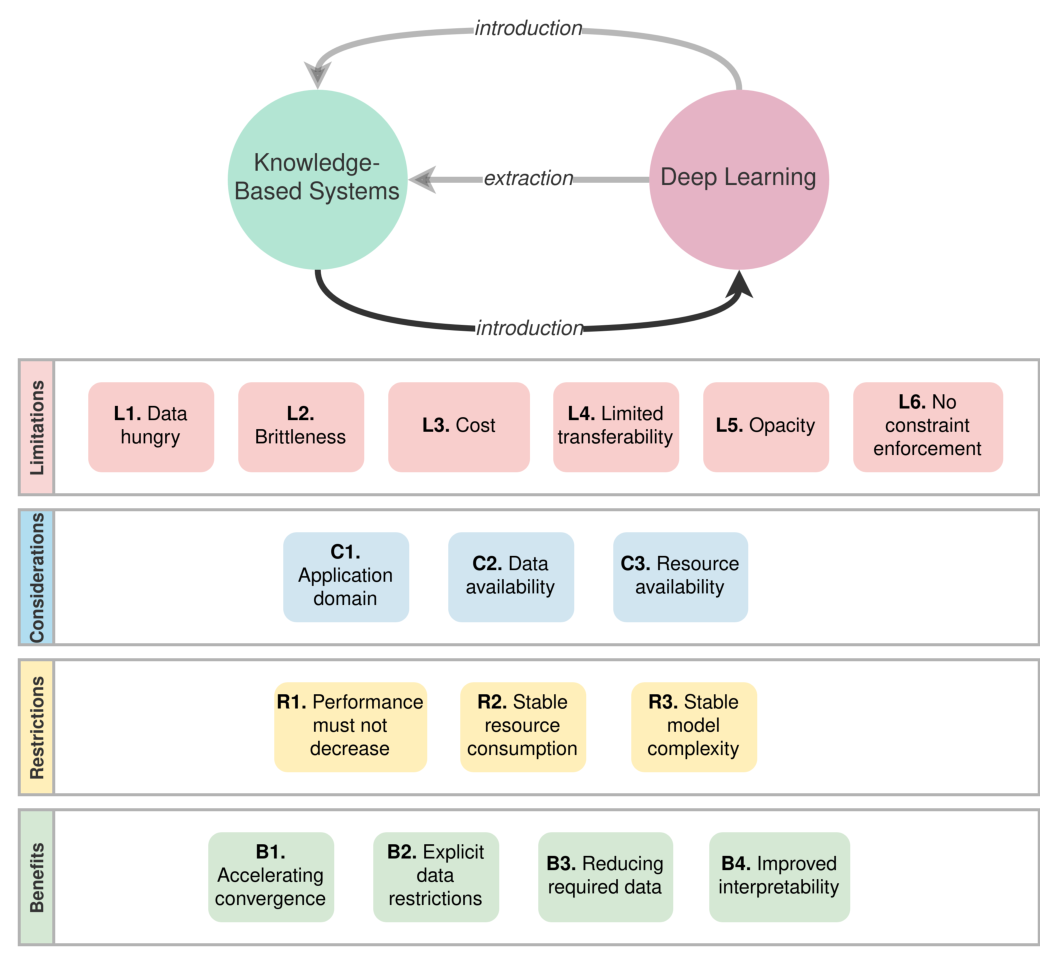
\includegraphics[width=\linewidth]{4_kbsintegrationdl/figures/overview_kbs_dl_intro.eps}
    \caption{Overview on the Insertion of Knowledge-Based Systems in Deep Learning.}
    \label{fig:overview_kbs_dl_intro}
\end{figure}

%%%LA MOVIDA DE LA SENSIA EN ESTA VERTIENTE CONCRETA
\section{Knowledge-Based System Insertion in Deep Learning Models} \label{4_sec:methodology_kbs_intro_dl}

\elvitodo{REFERENCIAR AL RESPECTO DEL CAPITULO 3}
In this scenario, the DL model plays the primary role, while the KBS plays the secondary role. Figure \ref{fig:overview_kbs_dl_intro} outlines the specific methodological parameters for this integration, which are defined as follows.

\paragraph{Limitations}
\begin{enumerate} [start=1,label={\bfseries L\arabic*.}]
    \item \label{kbsintrodl_L_data_hungry} \textbf{Data hungry.} This is one of the most concerning issues regarding DL. While DL is capable of achieving a better abstraction and generalization capacity than its symbolic counterpart, the final performance is highly linked to both the quality and the quantity of the data. Large, balanced, and representative training sets are required for the DL model to learn accurate patterns about the data. This limitation implies that the final performance of the model is directly bounded to its training data, thus not being a trusty indicator on the aptness of the model. 
    
    \item \label{kbsintrodl_L_brittleness} \textbf{Brittleness.} DL models infer abstract reasoning patterns from the training data. These patterns, however, may not be robust enough to correctly deal with noise. Adversarial attacks can cause DL models to fail. Therefore, even if a given DL produces an output $Y$ for a given input $X$, it can not be ensured that for a slightly corrupted version $X'$ of the input will lead to the same outcome.
    
    \item \label{kbsintrodl_L_cost} \textbf{Cost.} Training a DL model requires an elevated computational cost. While GPUs and TPUs have greatly alleviated this issue, the disparity on the availability of computational resources is a significant drawback of DL models. Not only the training time varies greatly across different infrastructures for the same implementation, but a given DL model may be incapable of training or executing if the available resources are insufficient. Maintaining computational cost at reasonable limits should therefore be prioritized.  
    
    \item \label{kbsintrodl_L_transfer} \textbf{Limited transferability.} Reusability is one of the most prominent features of DL models. Transfer learning reduces the need to retrain a given architecture from scratch to fit a new dataset or solve a new task. However, a model $M$ may achieve a remarkable performance on a given task $t$, but this performance may not  hold for a different task $t'$, even if they are fairly similar. Additionally, if a model $M'$ is trained using $M$ as a base, it can not be ascertain whether the performance of the newly trained model will be similar to the baseline.
    
    \item \label{kbsintrodl_L_opacity} \textbf{Opacity.} One of the main concerns regarding DL models is their limited explainability. DL models often provide better results than KBS on multiple tasks, but their usage is often hindered due to the impossibility to provide human-understandable insights on why a certain output is obtained.
    
    \item \label{kbsintrodl_L_constraint} \textbf{No constraint enforcement.} DL models infer patterns from a set of training samples. However, these patterns may not truthfully represent the data, as noisy or unbalanced data may negatively impact the learning process. The patterns learned by a DL model can then be inconsistent, and may not be able to properly generalize from unseen data.
    \end{enumerate}
\paragraph{Considerations}
\begin{enumerate} [start=1,label={\bfseries C\arabic*.}]
    \item \label{kbsintrodl_C_domain} \textbf{Application domain.} Table \ref{tab:sensors_reasoning} showcased an existing bias in the employed reasoning models according to their application. Complex and opaque approaches were selected in domains where their worst-case scenario impact was low (i.e. housing), while fully expressive and interpretable models were considerably favoured in human-dominated areas (i.e, healthcare). Therefore, in this scenario where the DL model is the primary, it must be studied whether the application domain strictly requires from human understandability. Even though the introduction of KBS into DL models may reduce its opacity, it may not be sufficient to fully comprehend the inference process of the model. 
    
    \item  \label{kbsintrodl_C_data} \textbf{Data availability.} As stated in \ref{kbsintrodl_L_data_hungry}, data availability is one of the main bottlenecks of DL models. This issue may be alleviated by the introduction of a KBS model. In those scenarios where the KBS model is already trained, data availability may not be an issue. However, if the KBS model needs to be trained before being integrated within the DL model, there must exists valid data to build the KBS model. Data availability for KBS model training must then be ensured beforehand.
    
    \item  \label{kbsintrodl_C_resource} \textbf{Resource availability.} This consideration is directly related to \ref{kbsintrodl_L_cost} (cost). KBS models have a much reduced computational cost in comparison to DL models. However, even if small, they still carry a computational cost that is added to the baseline cost of the DL model which should be noted. The cost of introducing the KBS model should never exceed the cost of the primary DL model.
    
\end{enumerate}
\paragraph{Restrictions}
\begin{enumerate} [start=1,label={\bfseries R\arabic*.}]
    \item \label{kbsintrodl_R_performance} \textbf{Performance must not decrease.} One of the fundamental strengths of DL models is that they provide remarkable performances on a wide variety of tasks. The introduction of a KBS model must never negatively impact the model performance, as this is a pivotal element that should therefore be preserved. While there may not be a remarkable improvement in the final metrics, for example, the correct prediction of outliers, which may represent a very small fraction of the data, the performance should, at least, remain stable.
    
    \item \label{kbsintrodl_R_resource} \textbf{Stable resource consumption.} The introduction of an additional model subsequently carries an additional cost. As noted in \ref{kbsintrodl_C_resource} (resource availability), this increment must be taken into consideration. The overall resource consumption of the model must remain within reasonable bounds (\ref{kbsintrodl_L_cost}), and the final model should be able to train and operate with the previously existing resources.
    
    \item \label{kbsintrodl_R_complexity} \textbf{Stable model complexity.} DL models are generally complex and suffer from elevated training times. Therefore, the KBS model should not add an additional complexity to the DL model. For this purpose, whenever possible, the KBS model must not be fully coupled with the DL model. Instead, it may be devised as an individual component that is actively involved in the training process of the DL model, but does not add any additional complexity to the model itself. 
    
\end{enumerate}
\paragraph{Benefits}
\begin{enumerate} [start=1,label={\bfseries B\arabic*.}]
    \item \label{kbsintrodl_B_convergence} \textbf{Accelerate convergence.} As noted in \ref{kbsintrodl_R_complexity}, DL models may suffer from elevated training times. This issue may be eased with the inclusion of a KBS, which already models knowledge about the data that the DL model may not even be capable of inferring otherwise. The introduction of this additional knowledge can not only lead to better performances, but reduce the training time as the model may converge faster to its optimal solution, reducing its computational cost (\ref{kbsintrodl_L_cost}).
    
    \item \label{kbsintrodl_B_restrictions} \textbf{Explicit data restrictions.} During training DL models internally learn restrictions and constraints about the data. As stated in \ref{kbsintrodl_L_constraint}, the implicit constraints about the data may be inconsistent, leading to errors. KBS extract explicit constraints and patterns from the data, which are then use to perform reasoning (e.g. rule-based systems, decision trees), that may not be inferred using a DL model. These restrictions can correct the behavior of the DL model for those inputs that can otherwise be subject to errors based on the internally learned patterns (\ref{kbsintrodl_L_brittleness}). 
    
    \item \label{kbsintrodl_B_reduce} \textbf{Reduce required data.} One of the main limitations of DL models (\ref{kbsintrodl_L_data_hungry}) is their high data availability requirement. On the contrary, KBS are capable to learn feasible inference patterns from reduced amounts of data. Subsequently, introducing a KBS in a DL model may reduce the training data required while still achieving accurate results. Moreover, it can improve the transferability of the final model (\ref{kbsintrodl_L_transfer}), as the DL model may keep its parameters constant while the KBS model is retrained for a new task. 
    
    \item \label{kbsintrodl_B_interpretability} \textbf{Improved interpretability.} The lack of explainability of DL models (\ref{kbsintrodl_L_opacity}) represents one of its main drawbacks. KBS, however, are generally fully explainable, interpretable and easily comprehensible by humans. Even when the inference process of the DL model may still be opaque, the introduction of a KBS may enable a certain degree of interpretability. Model outputs may not be fully explained, but some insights on the inference process based on the KBS information may be extracted.
    
\end{enumerate}

\section{Ontology Introduction to Knowledge Graph Embedding Models for Knowledge Graph Completion} \label{4_sec:ontointro_kgc}

%Knowledge Graph Completion (KGC) is one of the main application scenarios of neurosymbolic integration. This Section presents a use case of an introductory integration of a KBS under a DL framework, as presented in \cite{amadoretalontodl}. This use case focuses on KGC, specifically on its resolution via Knowledge Graph Embedding (KGE) models. As stated in Section \ref{sec:the_ai_spectrum}, KGE models generate vector representations for KGs, subsequently enabling statistical reasoning over the KG. In this scenario, a KG (structured, symbolic) serves as input. A KG is represented as a set of facts of the format \textit{(s,p,o)}, where $s,o \in \mathcal{E}$ and $r \in \mathcal{R}$, being $\mathcal{E}$ and $\mathcal{R}$ the entity and relation sets, respectively. The embeddings learned by the KGE model can then be used to infer new potential elements of the KG. 
%Following the standard model generation procedure, the input is divided into three separate subsets of facts: training, validation, and test, each containing a different set of facts from the KG. The training set is then fed into a KGE model, which generates a subsymbolic representation for each element of the input. 

Knowledge Graph Completion (KGC) is one of the main application scenarios of neurosymbolic integration. While KGE models provide an efficient solution for KGC, two main shortcomings can be identified: i) they only rely on the information explicitly declared in the input data, thus not considering background, general information that can lead to the inference of general restrictions, and ii) they cannot reason over inputs that were not seen by the model during training time. One of the main reasons behind these flaws is the training strategy employed by KGE models, as they rely on a local search strategy instead of a explorative one. Therefore, scalable and explorative approaches are needed to reason over the so-called \textit{out-of-knowledge-based} (OOKB) entities. This term is employed to refer to entities that were not featured in the training set and, therefore, have no representation. 

A feasible solution to this issue lies in the inclusion of explicit ontological information, as explored in \cite{Patrick}. Ontologies are a core element of the KG, serving as a scaffold for its generation as well as providing explicit restrictions about entities and relations. However, their use scope is limited exclusively to the generation and introduction of new elements of the KG \citep{paulheim2017knowledge}. Existing proposals regarding OOKB entity introduction include works such as \textit{puTransE} by \cite{putranse}, \textit{DKGE} by \cite{dkge}, \cite{hamaguchi_etal} and \cite{shah_open-world_2019}. These proposals, however, rely on deep learning models, thus suffering from the previously outlined limitations. This chapter presents a simpler, hybrid alternative to the aforementioned works, which eliminates the detected limitations while being easily integrated with any existing KGE model.


KGE models assign a singular representation for each entity and relation which encode the knowledge about the input derived from the training facts. While every entity is unique and this must be reflected in its representation, certain generalizations about them can be stated from the existing facts. Ontologies encode these generalizations and restrictions, and its inclusion alongside KGE models can enable the extraction of general patterns about facts while still maintaining the specificity of entities and relations. Additionally, ontologies play a key role in entity introduction, thus making this information about unseen entities easily available.

\begin{figure}
    \centering
    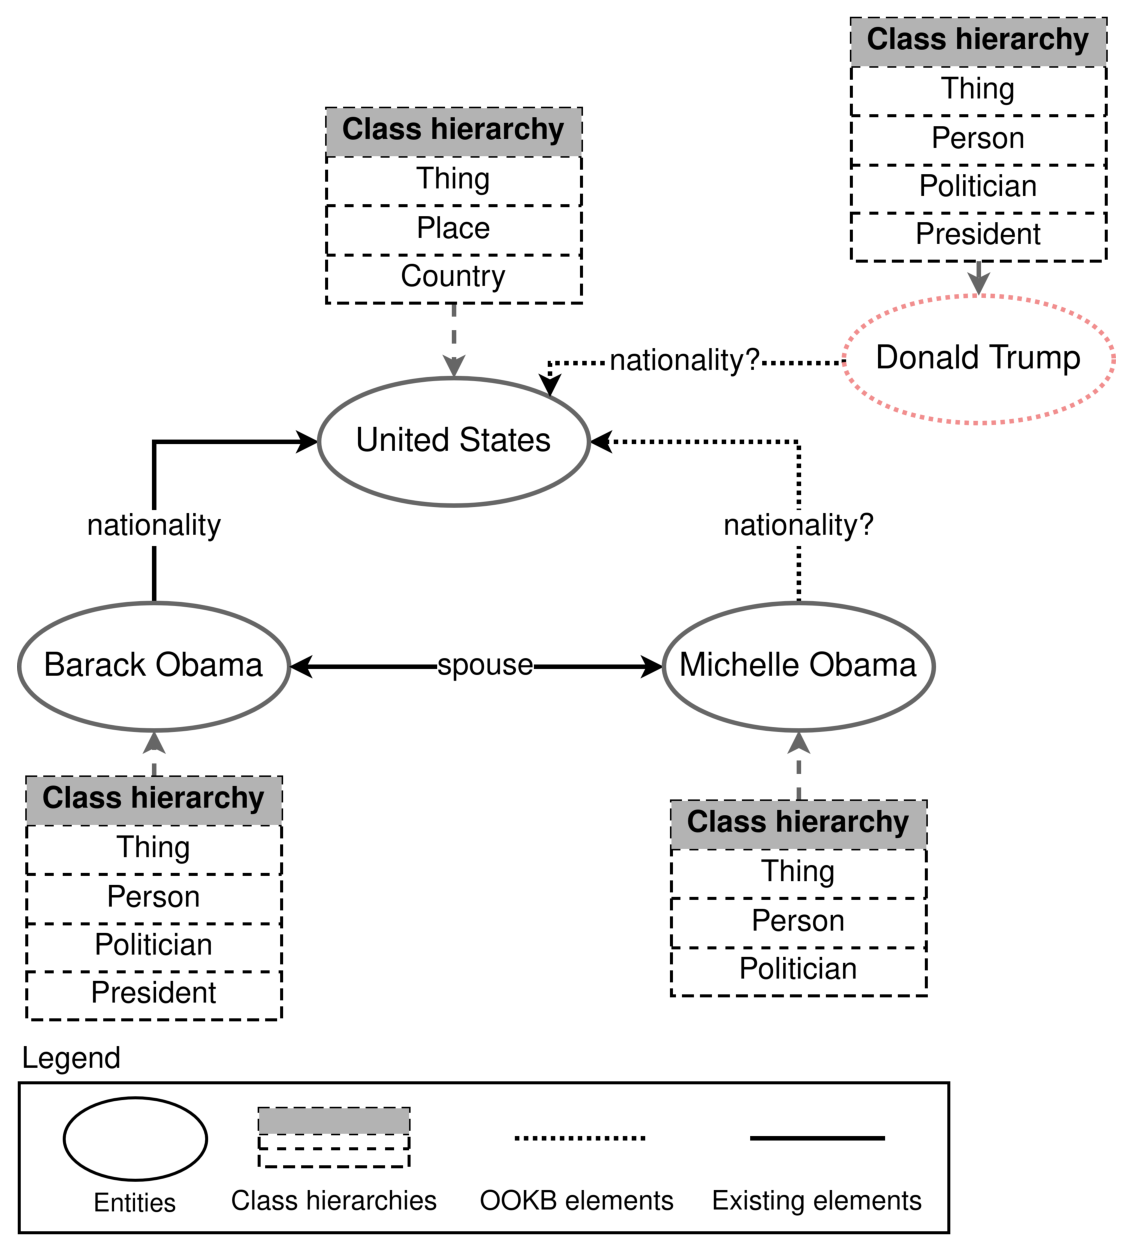
\includegraphics[width=.6\linewidth]{4_kbsintegrationdl/figures/KGCexample.eps}
    \caption{An example of KGC combining entity information and hierarchical information.}
    \label{fig:kgc_onto_example}
\end{figure}

Figure \ref{fig:kgc_onto_example} outlines the general idea of the proposal. Every entity contains its own ontological information. In this example, the class hierarchy of each entity is used as ontological information. While facts about a given entity $e$ are volatile and subject to change, its class hierarchy remains reasonably static throughout time. Moreover, class hierarchies are similar or even equal in those entities representing closely related concepts. \textit{Barack Obama} ($e_1$) and \textit{Donald Trump} ($e_2$) class hierarchies are equal, implying that they represent the same type of concept. For the entity \textit{Michelle Obama}, its class hierarchy is a subset of the class hierarchy of the aforementioned entities. Therefore, even though this entity does not represent a \textit{President}, it still holds a high resemblance with both $e_1$ and $e_2$. Considering the equality of the class hierarchies of entities $e_1$ and $e_2$, even though $e_2$ was not featured in the training set, analogical inference can be performed. The combination of the ontological background of the entity with its specific information makes it possible to leverage information about similar entities, leading the model to infer restrictions capable of enabling reasoning over OOKB entities. In the example depicted in Figure \ref{fig:kgc_onto_example}, even though the only known information about the entity \textit{Donald Trump} is its class hierarchy, it can be assessed whether the potential fact \textit{(DonaldTrump, nationality, UnitedStates)} holds based on its resemblance with the known fact \textit{(BarackObama, nationality, UnitedStates)}. 

%%%INICIO BLOQUE PAPER

\subsection{Semantic-Based Initialization for Out-Of-Knowledge-Base Entity Reasoning}

\label{4_sec:semantic_initialization}
\begin{figure}
    \centering
    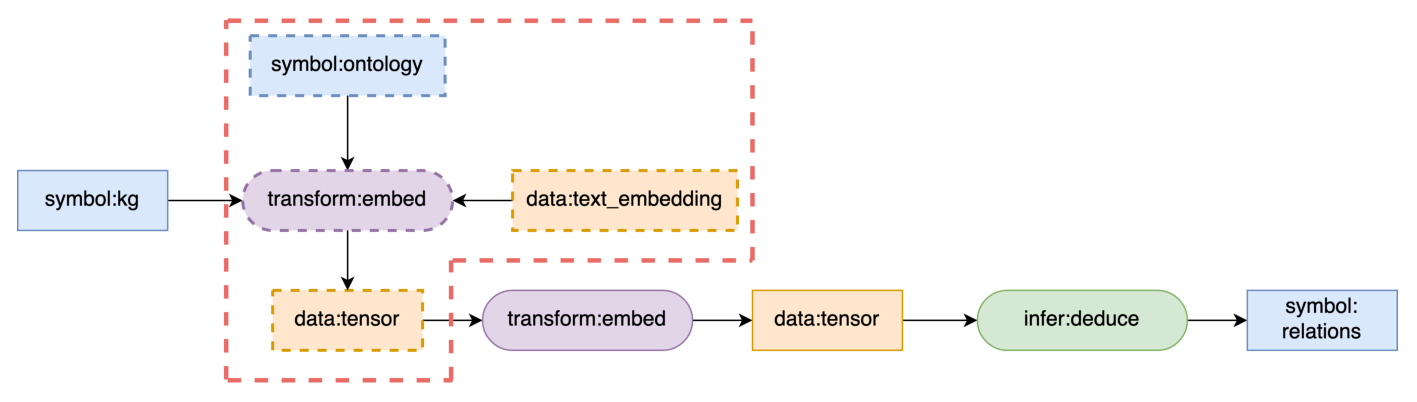
\includegraphics[width=\linewidth]{4_kbsintegrationdl/figures/VanBekkum_KGEOnto.eps}
    \caption{Boxology representation of the proposed hybrid KGE model. Dashed lines are used to highlight the added elements with respect to the baseline (Figure \ref{fig:van_bekkum_kgc_kge}).}
    \label{fig:box_krintodl}
\end{figure} 

Even though the introduction of ontological information solves the issue of OOKB entity reasoning, specific information about the unseen entities is also required to properly typify them. Moreover, unseen entities need to be represented in the same format as known entities to be processed by the KGE model. Figure \ref{fig:box_krintodl} shows the boxology representation of the proposed approach. Instead of directly feeding a set of facts in relational format to the KGE model like in the baseline model, an additional transformation layer is added to perform initialization (depicted as a red box). The proposed initialization method encodes not only ontological information, but specific semantic knowledge about each of the entities. From a formal representation standpoint, the proposed hybrid model may be perceived as more complex due to its increased number of boxes. However, it is worth noticing that the initialization is performed offline, thus not adding any complexity to the KGE model itself. Figure \ref{fig:semantic_based_initialization} depicts the three phases of the initialization: \textit{ontology retrieval}, \textit{entity knowledge encoding} and \textit{embedding composition}.

\begin{figure}
    \centering
    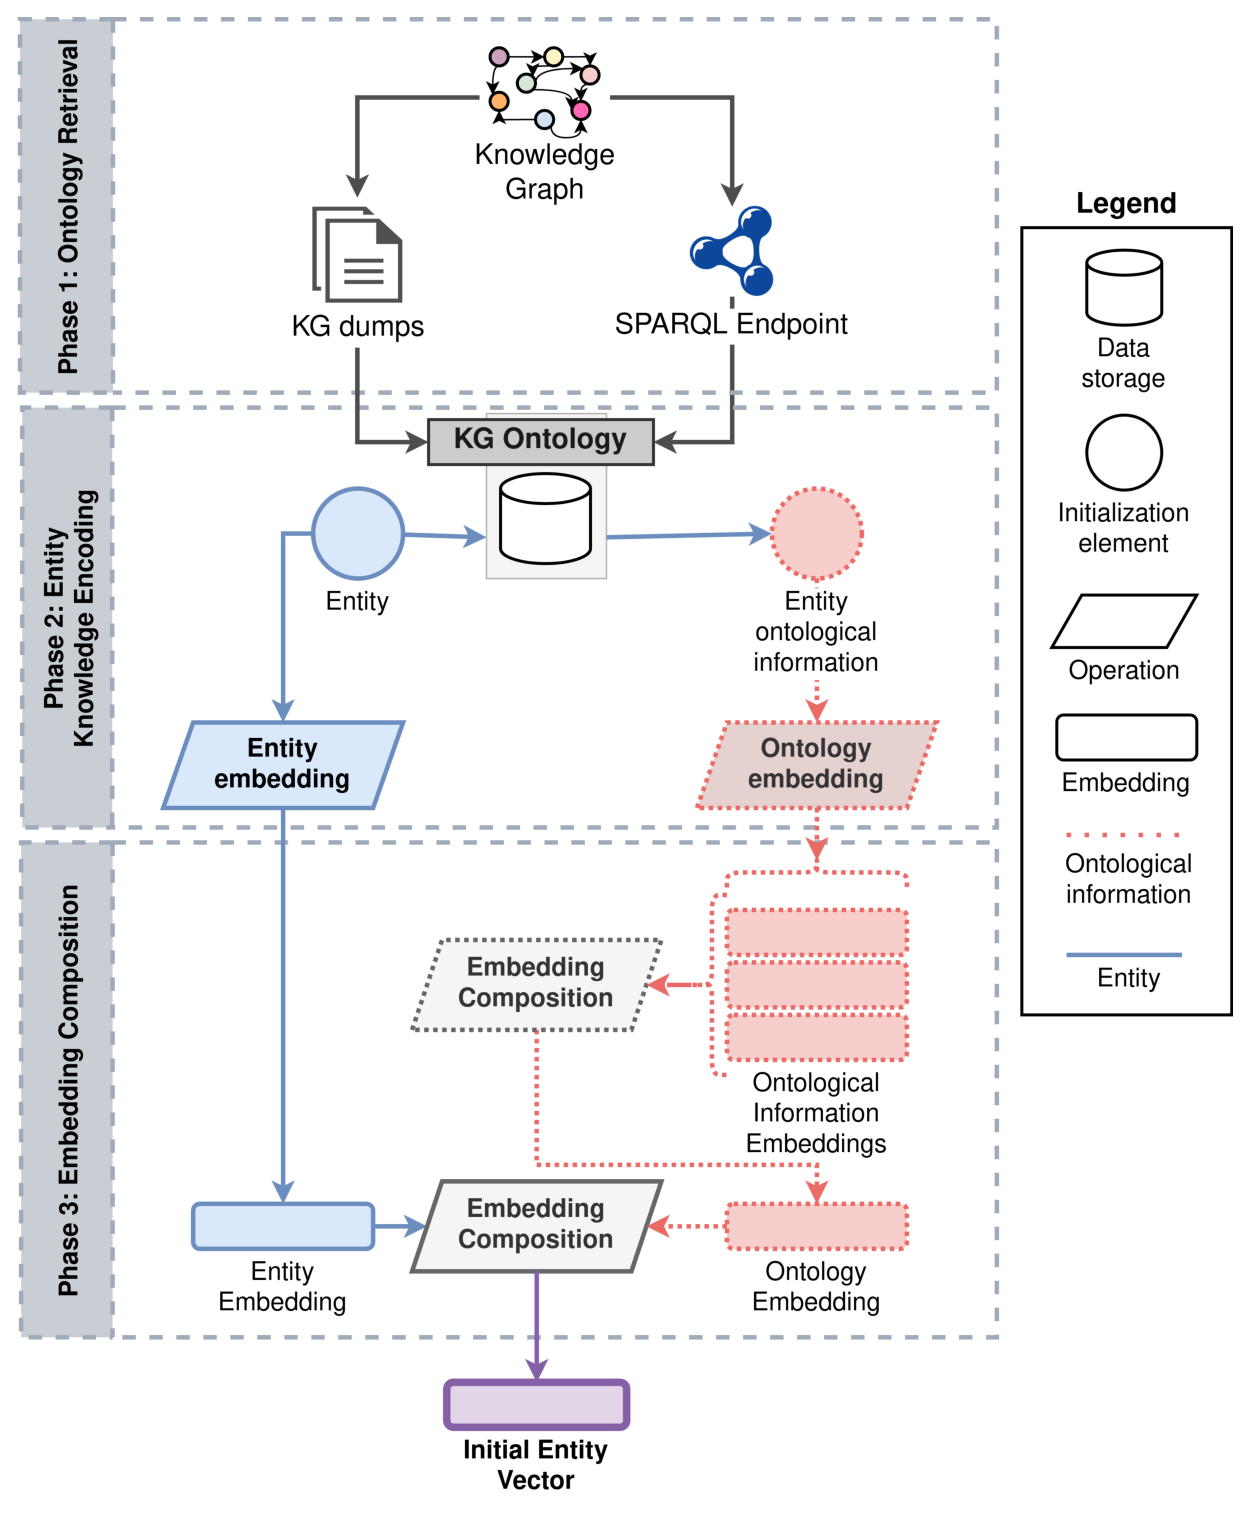
\includegraphics[width=.9\linewidth]{4_kbsintegrationdl/figures/Initialization_phases.eps}
    \caption{Overview of the three entity initialization phases.}
    \label{fig:semantic_based_initialization}
\end{figure}

\subsubsection{Theoretical Background.} \label{subsec:s4_theoretical_back}
As previously described, the purpose of KGE models is to subsymbollically represent the knowledge encoded in the KG, associating each entity and relation with a unique representation. One of the key features of the generated embeddings is that elements representing similar concepts must lead to similar encodings. From a technical standpoint, this constraint implies that if a pair of elements are conceptually similar, their corresponding embeddings should be close in the embedding distance. KGE models use specific scoring functions to ensure this restriction is met. While scoring functions vary amongst KGE models, two main categories can be defined: translational and bilinear. 

\begin{figure}[t!]
    \centering
    \subfigure[Translational model \label{fig:translational}]{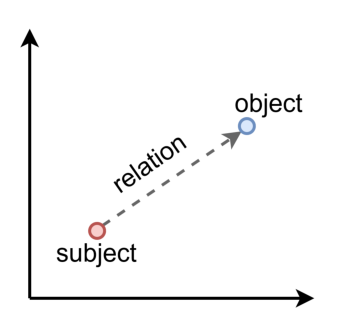
\includegraphics[height=1.5in]{4_kbsintegrationdl/figures/translational.eps}}
    \qquad
    \subfigure[Bilinear model \label{fig:bilinear}]{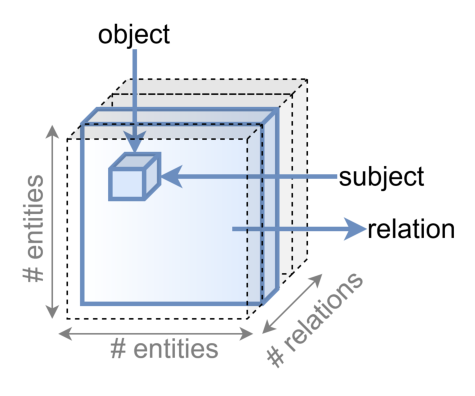
\includegraphics[height=1.5in]{4_kbsintegrationdl/figures/bilinear.eps}}
    \caption{Overview of the two main types of KGE models.}
    \label{fig:kge_overview}
\end{figure}

Translational models employ distance-based scoring functions. Figure \ref{fig:translational} depicts the core idea of translational models, where the relation between the subject and object entities is perceived as a translation operation. Entities and relations are modeled as vectors in ${\mathbb{R}}^{k}$, where $k$ is the dimension of the embeddings. As relation vectors $p$ are perceived as translation operations, a given fact $(s,p,o)$ holds when the distance between the embeddings $s+p$ and $o$ is minimal. The scoring function in Equation \ref{eq:trans_score} is formulated under the aforementioned constraint, which ensures that higher scores are assigned to lower distances:
\begin{equation}\label{eq:trans_score}
    f_p(s,o)=\|s + p - o\|_n
    \quad
    ( n \in \{1,2\})\,.
\end{equation} 

Bilinear models compute the plausibility of a given fact from the latent semantics and correlations existing between entities and relations. Figure \ref{fig:bilinear} showcases the foundation of bilinear models, where the KG is depicted as a tensor of dimensions $N_{entities} \times N_{entities} \times N_{relations}$. Each slice of the tensor models the pairwise interaction between the existing entities for a given relation $r$. Opposite to translational models, relations are depicted as matrices in $\mathbb{R}^{k_x k}$, where $k$ is the dimension of the embeddings. Entities follow the same representation criteria as translational models. Equation \ref{eq:bilinear_score} defines the scoring function employed by these models, where $M_p$ is the relation matrix , and $s$ and $o$ are the subject and object vector embeddings, respectively.

\begin{equation}\label{eq:bilinear_score}
    f_r(s,o)=s^T M_p o \,.
\end{equation}


%%%LOS RELATED WORKSSS
% The incremental six-step initialization procedure is depicted in Figure \ref{fig:overview}. These steps can be grouped into three different phases: \textbf{entity information retrieval, embedding generation} and \textbf{performance evaluation}


% Figure \ref{fig:overview} showcases the proposed incremental six-step procedure conducted to initialize and reason over OOKB entities. 
% \elvitodo{A lo mejor esa figura se podría modernizar, que está fea} These steps can be categorized into three phases: entity information retrieval, embedding generation and performance evaluation.

\subsubsection{Ontology Retrieval.} \label{subsec:s4_onto_retrieval}
Opposite to the volatility of KGs, ontologies provide stable, general information. Their role in the generation of KGs is crucial, but their application scope is usually limited to the introduction and creation of new elements of the graph. The information encoded in ontologies can be particularly beneficial for KGC, as they provide explicit restrictions about the type of entities featured in each relation, as well as additional information that can boost the inference process.

Ontologies comprise the following parts: individuals, classes, properties, relations, function terms, restrictions, rules, axioms, and events. Only individuals (or entities in the context of KGs), relations, and properties are considered by KGE models for the generation of representations. Therefore, a substantial number of components that could improve the final quality of the embeddings is dismissed.

Class hierarchies are at the core of both ontologies and KGs. During the introduction, entities are grouped into the class that better represents them conceptually. Classes are not atomic, but form a tree-like hierarchical structure, ranging from the most specific (or \textit{leaf}) classes to the \textit{root} class, which is shared by all entities in the graph. This taxonomical structure enables fine-grained distinctions between conceptually similar classes, as in Figure \ref{fig:kgc_onto_example}, where the entities \textit{Barack Obama} and \textit{Michelle Obama} are both \textit{Politicials}, but the first one is also a \textit{President}. Therefore, it provides a trade-off between the generality of the tree-like structure with the specificity of the different subclasses. 

While classes provide a general and unified framework, properties provide distinct, unique information about entities. KG facts are usually extracted from the interaction between two individuals by means of a property. Properties that relate an individual with a non-individual (i.e: a numerical value, a description, etc.) are usually discarded, even though this information could further enrich the final embeddings. Rules and axioms can also be encoded within the KGE model. In this case, axioms can be used to guide the training of the KGE model, ensuring the consistency of the predictions. Additionally, rules can also be used for training data augmentation, as new facts may be inferred from the existing KG. The newly inferred facts can then also be included as part of the training set.

Restrictions are also closely related with KGEs, as relation representations encode implicit constraints about the expected types of subject and object entities. However, the restrictions inferred by KGE models have a local scope, as they are based only on the facts contained in the training set. Therefore, these constraints may not be applicable to every fact that features the relation. Explicit restrictions about the relations can also be encoded jointly with their representations to deal with this shortcoming, improving the performance of the model on KGC.

Phase 1 of Figure \ref{fig:semantic_based_initialization} illustrates two different available paths for ontology retrieval: KG dumps or SPARQL queries. Currently, most of the publicly available KGs provide their data dumps, which includes not only the KG facts, but its ontology file along with extra documentation. Every entity and relation encoded in the KG is explicitly related to its corresponding ontological information, which reduces the retrieval time. Data dumps usually come compressed in a single file that can scale up to several terabytes, which can be undesirable in terms of computational resources. KGs usually provide a SPARQL endpoint, which enables information retrieval via queries. This approach is more efficient, as fewer resources are required and the target information can be retrieved directly with a single query. Nonetheless, using SPARQL queries may be discouraged in cases where the KG has a large size or if the number of SPARQL queries is elevated. 

\subsubsection{Entity Knowledge Encoding.}\label{subsec:s4_entity_encode}
The first phase of the proposed initialization focuses on obtaining the ontological information required to categorize each entity. While the existing OOKB entity reasoning approaches presented in Section \ref{4_sec:ontointro_kgc} are capable of generating highly representative embeddings, these representations lack any semantic information about the entity itself. Semantic information is highly relevant in this context, as it enriches the entity embeddings with an additional level of knowledge that can not be inferred otherwise. Despite this fact, most KGE models still rely on random initialization. 

One-hot vectors are an easy and straightforward replacement for random initialization. In this encoding, each entity is embedded as a vector of dimension $N$, where $N$ is the total number of entities. For every entity, a single vector can be created composed entirely of zeros except for a single one value in a given position, which is unique to each entity. While this encoding may be suitable for small KGs, it cannot be applied to large inputs, as the dimension of the embedding grows linearly with the size of the KG. Moreover, zero-valued initializations can hinder the convergence of the model to its optimal solution, and they do not encode semantic information about the entity.

Language models are a potential initialization alternative. These methods are capable of generating expressive, unique representations for words. Different paradigms can be identified amongst language models for the representation of words. Word2Vec \citep{word2vec} generates a single representation per token in the vocabulary, which hinders the representation of unseen words. FastText \citep{fasttext1,fasttext2} considers each word as a set of subparts called n-grams, assigning a representation for each of them. The final representation of a word is composed by the average of this n-grams. While FastText is capable of representing words that were not in the training corpus and still enable analogical reasoning, it still lacks the capability of correctly model polysemy. Language models, such as ElmO \citep{elmo} or BERT \citep{bert} solve all of the aforementioned issues, but the dimension of the resulting embeddings increases noticeably. Word2Vec embeddings tend to have a length of about 300, which scales up to 2048 on BERT. This dimension conflicts with the regular dimension of KGE vectors, which rarely exceed 200. Dimensionality reduction based on principal component analysis is a potential solution to the mismatch between the dimensions of KGE and word embedding outputs. However, it must be noted that reducing the dimension of a word embedding directly can affect its final expressivity. 

Another important dissimilarity between word and KG embeddings is that whereas word embeddings follow a token-based approach, KGE models are oblivious to the number of tokens that name an entity. Therefore, a composition method is needed that guarantees that all tokens that compose an entity are represented on its initial embedding. A potential solution for this issue would be to concatenate single representations of each entity token to generate the initial entity embedding. However, this solution is not feasible in the context of KGEs, as all entity embeddings must be equally dimensional. Averaging token representations to generate the initial entity embeddings provides a more fitting solution to this case.

The encoding process of this phase is outlined in Figure \ref{fig:semantic_based_initialization}. Alongside the initial entity embedding, feasible encodings for the ontology are also generated in this phase. The encoding of the ontological information depends on two factors: i) the type of ontological information selected, and ii) the targeted component of the KG (entity or relation). 

Class hierarchies only encompass entities, which are modelled as vectors by most KGE models. Therefore, a vector encoding must be also employed to represent class hierarchies. The simplest feasible solution uses one-hot vectors of dimension $O$, where $O$ is the number of classes that comprises the ontology. While simple, this representation is suitable for representing the class hierarchy of each entity, as it ensures the maintenance of the similarity between the embeddings of the classes of similar entities. Although valid, this codification presents two main shortcomings: i) it lacks semantic information about the concept represented by the class, and ii) its dimension grows linearly with the number of classes in the ontology. Word embeddings can also be used for class hierarchy embedding. In this scenario, each ontology class is encoded using its corresponding word embedding.

In the case of relations, matrices can be used for restriction encoding. Each relation can be codified as a matrix of dimensions $C \times C$, where $C$ is the total of leaf classes and restrictions that can be encoded using binary vectors. If the head class $i$ is restricted to the tail class $j$ through a relation, the cell $(i,j)$ should have a positive value denoting this restriction, and zero otherwise.



\subsubsection{Embedding Composition.} \label{subsec:s4_embedding_compo}
In this stage, semantic and ontological information are combined to generate the initial value of the entity, as shown in Figure \ref{fig:semantic_based_initialization}. First, the embeddings of the ontological information about the entity are flattened into a single representation. In the context of class hierarchies, an entity can belong to several different classes, each with a unique representation. Hence, the embeddings of the entity classes must be combined into a single embedding. Different vector composition techniques can be used for this task. Averaging all class embeddings is one potential solution, although this approach does not encode the hierarchical information of the ontology classes. Weighted average can be used instead, potentially introducing the hierarchical properties of the ontology in the final representation.

As stated in the previous phase, the encoding method must be aligned with the target component of the KG. If the ontological information is embedded alongside the KGE, then the encoding method must be compliant with the dimension restrictions of the model. While in this initialization the focus is on entity embeddings, the same restriction applies for relations. Three composition procedures can be employed to combine the ontological information alongside the embeddings of the KGE model:
\begin{itemize}
    \item \textit{Concatenation:} The simplest approach is to append the representations of each class to generate a high-dimensional embedding. This procedure ensures that a section of the embedding remains static throughout the training, and that its equal across entities that share ontological information. This ensures a similarity in the final representations of similar entities. Therefore, if the dimension specified by the KGE model for the embeddings is $d_T$, the following constraint must be met:
    \begin{equation}
        d_O+d_M=d_T\,,
    \end{equation}
    where $d_M$ is the dimension of the entity embeddings and $d_O$ is the dimension of the ontological information embedding. In this scenario, $d_O$ and $d_M$ are not required to have the same dimension. While this approach is suitable for the problem, the training time of the model increases due to the growth in the embedding size. Additionally, the optimal dimensions for the ontological and entity representations must be determined beforehand to ensure a fair tradeoff between general and specific knowledge.
    
    \item \textit{Average:} In this approach, both representations are averaged into a single embedding. Therefore, both entity and ontological representations must have the same dimension, following the constraint:
    \begin{equation}
        d_T = d_O = d_M.
    \end{equation}
    The simplest way to ensure this condition is met is to use the same embedding model for both entity and ontology embeddings. Otherwise, either reduction or zero-padding may be necessary to ensure that both representations have the same dimension before averaging them. This approach assigns equal importance to general and specific information. As all embedding dimensions are equal in this scenario, performing dimension reduction is less penalizing than in the previous case.
    
    \item \textit{Weighted Average:} While averaging solves the dimensionality problem existing in the concatenation option, this technique is still oblivious to the balance between general and specific information. Weighted average solves this issue, enabling the possibility of assigning different relevance values to specific and ontological information. While averaging and assigning the same weight to both representations may be perceived as the fairest approach, it may not be optimal for the performance of the KGE model. As in the previous case, both entity and ontological information embeddings must have the same dimension. In addition, the following composition constraint must be met:
    \begin{equation}
        T = \frac{\lambda \times O + (1 - \lambda) \times M}{2}\,,
    \end{equation}
    where $T$ is the final representation, $\lambda$ is the assigned weight, and $O$ and $M$ are the ontological information and entity embeddings, respectively. This method maintains the balancing benefits of concatenation while maintaining a stable dimension for the embeddings. Nonetheless, it rises a new challenge: computing the optimal value of $\lambda$. This value can be manually defined or treated as an additional training parameter to optimize.
\end{itemize}

The proposed initialization approach is model-agnostic, and can subsequently be encoded alongside any KGE model. However, from a conceptual standpoint, it may not be suitable for any proposal. In translational models, optimization is performed by reducing the distance between the result of a translation operation and a target value, following an entirely arithmetic approach. As neither latent semantics nor correlations are considered, the introduction of ontological information may be detrimental for the performance of the model.

Bilinear models base their predictions on the exploitation of latent semantics and implicit correlations between elements. Enriching the semantic information available to the model during training time can potentially be translated into an improvement on its performance. Moreover, the inclusion of ontological information can add an exploratory layer to KGE models in addition to their exploitative behavior.

\subsection{Evaluation}\label{4_sec:experiments}
%%AQUI EXPLICAMOS YA LOS MODELOS EXACTOS SOBRE LOS QUE SE EVALUA Y LOS DATASETES
\begin{table}[h]
\resizebox{\linewidth}{!}{
\begin{tabular}{|c|c|c|c|c|}
\hline
\textbf{Model name} & \textbf{Model type}        & \begin{tabular}[c]{@{}c@{}}\textbf{Embedding} \\ \textbf{Dimensions}\end{tabular} & \begin{tabular}[c]{@{}c@{}}\textbf{Scoring} \\ \textbf{Function}\end{tabular} & \begin{tabular}[c]{@{}c@{}}\textbf{Complexity} \\ \textbf{Order}\end{tabular}\\ \hline
TransE \citep{transe}    & Translational &\begin{tabular}[c]{@{}c@{}}$h,t \in \R ^d$ \\ $r \in \R ^d$\end{tabular}  &$- {\lVert h + r - t \rVert}_{\frac{1}{2}} $&$\mathcal{O}(d)$\\ \hline
DistMult \citep{distmult}   & Bilinear & \begin{tabular}[c]{@{}c@{}}$h,t \in \R ^d$ \\ $r \in \R ^d$\end{tabular}  & $h^Tdiag(r)t$&$\mathcal{O}(d)$\\ \hline
ComplEx \citep{complex}    & Bilinear &\begin{tabular}[c]{@{}c@{}}$h,t \in \C^d$ \\ $r \in \C^d$\end{tabular} & $Re(h^T diag(r) \compconj{t})$ &$\mathcal{O}(d)$\\ \hline
ANALOGY \citep{analogy}    & Bilinear &\begin{tabular}[c]{@{}c@{}}$h,t \in \R ^d$ \\ $r \in \R ^d$\end{tabular} &$h^T M_r t$&$\mathcal{O}(d)$\\\hline
SimplE \citep{simple}    & Bilinear & \begin{tabular}[c]{@{}c@{}}$h,t \in \R^d$ \\ $r,r^{-1} \in \R^d$\end{tabular}& $\frac{1}{2}[(h r t^T) + (h r^{-1} t)] $&$\mathcal{O}(d)$\\ \hline
\end{tabular}

\caption{Summary of the models considered for evaluation. Head and tail entity embeddings are shown as \textit{h} and \textit{t}, respectively. Relations whose embedding is vectorial are represented by an \textit{r}, while relation matrices are defined as $M_r$. The embedding dimension is denoted by \textit{d}. \label{tab:kge_experiment_model_summary}} 
}
\end{table}

The proposed initialization model is evaluated on five different KGE models. Considering the semantic nature of the proposed method, the experimentation primarily focuses on bilinear models. Table \ref{tab:kge_experiment_model_summary} summarizes the properties of each model. Section \ref{4_sec:ontointro_kgc} provided some references of approaches capable of performing OOKB entity reasoning. However, these approaches are not directly comparable with the method proposed due to a fundamental conceptualization difference. The proposals presented in Section \ref{4_sec:ontointro_kgc} are KGE models themselves, specifically designed for OOKB entity reasoning. On the contrary, the proposed method is not a KGE model by itself, and can be implemented across a wide variety of KGE models. In semantic-based initialization, OOKB entity reasoning is an induced benefit, but the final goal is to encode explicit background knowledge to overcome the existing limitations within KGE models.

Semantic-based initialization is evaluated on two triple classification datasets: FB13 \citep{neuraltensornetwork,Bollacker:2008:FCC:1376616.1376746} and WN11 \citep{Miller95wordnet:a}. These datasets contain facts from 13 and 11 relations extracted from Freebase and WordNet KGs, respectively. For each model reported in Table \ref{tab:kge_experiment_model_summary}, the optimal parameters reported by their authors are used. Similarly, the optimization algorithms recommended by the original authors are used: Adam \cite{adam} for FB13, and ADAGRAD \cite{adagrad} for WN11.

Triple classification is used to evaluate  the semantic-based initialization. Three different metrics are reported to assess the performance of the different KGE models in combination with the proposed initialization:

\begin{itemize}
    \item \textit{Recall} determines the proportion of true facts that are actually evaluated as true by the KGE model. Being \textit{TP} and \textit{FN} the number of true facts correctly and incorrectly classified respectively, recall can be computed as:
    \begin{equation}
        Recall = \frac{TP}{TP+FN}
    \end{equation}
    
    \item \textit{Average Precision (AP)} weights precision and recall increment of the model across different threshold values $t$. It provides an overall measurement of the model's classification while penalizing biased predictions. It is calculated as follows:
    \begin{equation}
        AP = \sum_{t} (R_t - R_{t-1}) \times P_t \,,
    \end{equation}
    where $R$ denotes the recall value, and $P$ represents the precision, computed as:
    \begin{equation}
        Precision = \frac{TP}{TP+FP} \,,
    \end{equation}
    \textit{FP} depicts the number of unfeasible facts predicted as true by the KGE model.
    
    \item \textit{F1 Score} is the harmonic mean between precision and recall, and serves as an indicator of the model's accuracy. It can be computed as:
    \begin{equation}
        F1 \; Score = \frac{2 (P \times R)}{(P + R)}
    \end{equation}
\end{itemize}

Semantic-based initialization is evaluated following an incremental approach. First, simple entity initialization is performed, replacing random initialization with word embedding based initialization. Simple entity initialization is then extended to include ontological information, which is embedded alongside the entities. Finally, semantic-based initialization is evaluated for OOKB entity reasoning.

\subsubsection{Simple Entity Initialization.}

\begin{table} 
\centering
\resizebox{.8\linewidth}{!}{
\begin{tabular}{l|c|c|c|c|c|c|}
\cline{2-7}
                                                                & \multicolumn{3}{c|}{FB13} & \multicolumn{3}{c|}{WN11} \\ \cline{2-7} 
                                                                & TCAP  & Recall & F1 Score & TCAP  & Recall & F1 Score \\ \hline
\multicolumn{1}{|l|}{\textit{ComplEx}}                          & 0.78  & 0.65   & 0.68     & 0.71  & 0.58   & 0.62     \\
\multicolumn{1}{|l|}{\textit{CompEx + SEI}}   & 0.76  & 0.64   & 0.67     & 0.76  & 0.6    & 0.64     \\ \hline
\multicolumn{1}{|l|}{\textit{DistMult}}                         & 0.71  & 0.61   & 0.64     & 0.68  & 0.58   & 0.61     \\
\multicolumn{1}{|l|}{\textit{DistMult + SEI}} & 0.71  & 0.61   & 0.64     & 0.68  & 0.58   & 0.61     \\ \hline
\multicolumn{1}{|l|}{\textit{TransE}}                           & 0.72  & 0.58   & 0.62     & 0.82  & 0.65   & 0.69     \\
\multicolumn{1}{|l|}{\textit{TransE + SEI}}   & 0.72  & 0.58   & 0.62     & 0.83  & 0.65   & 0.69     \\ \hline
\multicolumn{1}{|l|}{\textit{ANALOGY}}                          & 0.65  & 0.52   & 0.58     & 0.67  & 0.58   & 0.59     \\
\multicolumn{1}{|l|}{\textit{ANALOGY + SEI}}  & 0.68  & 0.58   & 0.61     & 0.68  & 0.56   & 0.6      \\ \hline
\multicolumn{1}{|l|}{\textit{SimplE}}                           & 0.77  & 0.65   & 0.67     & 0.48  & 0.49   & 0.49     \\
\multicolumn{1}{|l|}{\textit{SimplE + SEI}}   & 0.74  & 0.64   & 0.67     & 0.6   & 0.53   & 0.55     \\ \hline
\end{tabular}}
\caption{Triple classification average precision. recall. and F1 score with and without entity initialization (marked as +SEI)}
\label{tab:exp_entity_init}
\end{table}

A pretrained Word2Vec model is used to obtain the initial embeddings for the entity set $\mathcal{E}$. By using a pretrained model, the computational cost of the proposal remains low. As stated in Section \ref{subsec:s4_entity_encode}, entities can be compound, while the selected Word2Vec model is tokenized. Therefore, given an entity $e \in \mathcal{E}$, its initial embedding is obtained by averaging all the tokens contained in $e$. First, the entity vocabulary $V$ is created, containing all unique entity tokens. For each token $t \in V$, its representation is extracted from the pretrained Word2Vec model, and stored in a dictionary of tuples of the form $(token, embedding)$.

The selected Word2Vec model provides 300-dimension representations. The KGE models selected for evaluation use embedding dimensions that range from 100 to 200. Dimension reduction based on principal component analysis is performed to fit the dimension of the token embeddings to 200. Then, for each entity $e \in \mathcal{E}$, its tokens $t \in e$ are extracted from the previously constructed dictionary and averaged afterwards to generate a single representation. Those entities where none of its tokens is contained in the Word2Vec model's vocabulary are initialized using a randomized normal distribution.

Table \ref{tab:exp_entity_init} reports the TCAP, F1 score and recall for each model with and without simple entity initialization (marked as + SEI).

\subsubsection{Semantic-Based Initialization.}
The class hierarchy of entities is selected as ontological information in the second experimentation stage, as it can be easily integrated within the previously initialized entity embeddings. SPARQL endpoints are used to retrieve the class hierarchy of each entity. For the entities in WN11, its homonym ontology is applied, which splits the entities into four classes according to their word type: nouns, adjectives, verbs and adverbs. For FB13, two different ontologies are considered. Freebase is currently integrated within the Google Knowledge Graph, thus inheriting its ontology. The GKG API was employed to retrieve the classes of each FB13 entity, identifying a total of 64 classes. The root class \textit{Thing} is assigned to those entities where no leaf classes are specified.

An additional ontology is considered for FB13 to study the existing dependency between the complexity of the class hierarchy and the results achieved by the KGE model. DBpedia ontology is selected, having a total number of 685 different classes. The DBpedia SPARQL endpoint is used to retrieve the class hierarchy of each entity. As this ontology is external to FB13, each entity's class hierarchy cannot be directly obtained. The SPARQL query in Listing \ref{lst:sparql} is executed for each entity, exchanging the label value according to each entity $e \in \mathcal{E}$. The class hierarchy of each entity is saved in a dictionary of tuples of the form $(entity, [classes])$. From the total 685 classes of the DBpedia ontology, only 197 are featured in the class hierarchies of the entities in FB13. As in the previous case, the root class \textit{Thing} is assigned to those entities where no class information is available.

\begin{lstlisting}[captionpos=b, float=tp,floatplacement=tbp, caption=Example of a SPARQL query used to retrieve the class hierarchy of the entity ``Albert Einstein''., label=lst:sparql,basicstyle=\ttfamily,frame=single]
PREFIX dbr: <http://dbpedia.org/resource/>
SELECT DISTINCT ?class
WHERE {
 ?item rdfs:label "Albert Einstein"@en .
 ?item rdf:type ?class.
 ?class a owl:Class.
}
\end{lstlisting}

After retrieving the class hierarchy of the entities, the same pretrained Word2Vec model employed for simple entity initialization is used for encoding the ontology classes. Similarly to the previous case, for those classes composed by more than one word, average composition is applied to generate a single representation per class. The embeddings of each class are stored in a dictionary of tuples of the form $(class, embedding)$. Dimension reduction is also performed on the class embeddings to ensure equality between the dimensions of the entity and ontological embeddings.

For each $e \in \mathcal{E}$, its list of classes $C$ is obtained. Then, for each $c \in C$, its corresponding embedding is retrieved is embedding from the corresponding dictionary, then averaged to produce a single representation. A matrix of dimensions $N_e \times d_T$ is obtained as a result, being $N_e$ the number of entities and $d_T$ the dimension of the KGE model embeddings. Each entity embedding is then averaged with its corresponding ontology embedding on each training iteration, generating a single representation per entity during training time. Whereas the entity embeddings are model parameters and are subsequently updated during training, ontology embeddings remain static. This constraint ensures that the ontological information of the entities remains constant and that the equality between the class hierarchies of similar entities is always met.

\begin{table} 
\centering
\resizebox{.85\linewidth}{!}{
\begin{tabular}{l|c|c|c|c|c|c|}
\cline{2-7}
\textit{}                                                                & \multicolumn{3}{c|}{FB13} & \multicolumn{3}{c|}{WN11} \\ \cline{2-7} 
\textit{}                                                                & TCAP  & Recall & F1 Score & TCAP  & Recall & F1 Score \\ \hline
\multicolumn{1}{|l|}{\textit{ComplEx + DBOnt}}                           & 0.65  & 0.6    & 0.62     & -     & -      & -        \\
\multicolumn{1}{|l|}{\textit{ComplEx + GKGOnt}}                          & 0.74  & 0.62   & 0.65     & -     & -      & -        \\
\multicolumn{1}{|l|}{\textit{ComplEx + WNOnt}}                           & -     & -      & -        & 0.75  & 0.58   & 0.64     \\
\multicolumn{1}{|l|}{\textit{CompEx + DBOnt + SEI}}    & 0.73  & 0.62   & 0.65     & -     & -      & -        \\
\multicolumn{1}{|l|}{\textit{ComplEx + GKGOnt + SEI}}  & 0.73  & 0.61   & 0.63     & -     & -      & -        \\
\multicolumn{1}{|l|}{\textit{ComplEx + WNOnt + SEI}}   & -     & -      & -        & 0.76  & 0.6    & 0.65     \\ \hline
\multicolumn{1}{|l|}{\textit{DistMult + DBOnt}}                          & 0.71  & 0.62   & 0.64     & -     & -      & -        \\
\multicolumn{1}{|l|}{\textit{DistMult + GKGOnt}}                         & 0.74  & 0.62   & 0.65     & -     & -      & -        \\
\multicolumn{1}{|l|}{\textit{DistMult + WNOnt}}                          & -     & -      & -        & 0.65  & 0.57   & 0.6      \\
\multicolumn{1}{|l|}{\textit{DistMult + DBOnt + SEI}}  & 0.71  & 0.62   & 0.64     & -     & -      & -        \\
\multicolumn{1}{|l|}{\textit{DistMult + GKGOnt + SEI}} & 0.75  & 0.61   & 0.62     & -     & -      & -        \\
\multicolumn{1}{|l|}{\textit{DistMult + WNOnt + SEI}}  & -     & -      & -        & 0.75  & 0.6    & 0.64     \\ \hline
\multicolumn{1}{|l|}{\textit{ANALOGY + DBOnt}}                           & 0.67  & 0.6    & 0.62     & -     & -      & -        \\
\multicolumn{1}{|l|}{\textit{ANALOGY + GKGOnt}}                          & 0.68  & 0.6    & 0.63     & -     & -      & -        \\
\multicolumn{1}{|l|}{\textit{ANALOGY + WNOnt}}                           & -     & -      & -        & 0.7   & 0.58   & 0.6      \\
\multicolumn{1}{|l|}{\textit{ANALOGY + DBOnt + SEI}}   & 0.67  & 0.6    & 0.62     & -     & -      & -        \\
\multicolumn{1}{|l|}{\textit{ANALOGY + GKGOnt + SEI}}  & 0.68  & 0.6    & 0.62     & -     & -      & -        \\
\multicolumn{1}{|l|}{\textit{ANALOGY + WNOnt + SEI}}   & -     & -      & -        & 0.64  & 0.55   & 0.59     \\ \hline
\multicolumn{1}{|l|}{\textit{SimplE + DBOnt}}                            & 0.63  & 0.6    & 0.61     & -     & -      & -        \\
\multicolumn{1}{|l|}{\textit{SimplE + GKGOnt}}                           & 0.76  & 0.63   & 0.66     & -     & -      & -        \\
\multicolumn{1}{|l|}{\textit{SimplE + WNOnt}}                            & -     & -      & -        & 0.6   & 0.55   & 0.57     \\
\multicolumn{1}{|l|}{\textit{SimplE + DBOnt + SEI}}    & 0.66  & 0.6    & 0.62     & -     & -      & -        \\
\multicolumn{1}{|l|}{\textit{SimplE + GKGOnt + SEI}}   & 0.74  & 0.61   & 0.65     & -     & -      & -        \\
\multicolumn{1}{|l|}{\textit{SimplE + WNOnt + SEI}}    & -     & -      & -        & 0.62  & 0.54   & 0.58     \\ \hline
\end{tabular}
}
\caption{Triple classification average precision per instance model with and without entity initialization and ontology introduction. For Freebase, two different ontologies are used: DBOnt refers to the DBpedia Ontology, and GKGOnt to the Google Knowledge Graph Ontology.}
\label{tab:exp_ont_intro}
\end{table}

This second experimentation stage is evaluated only on the bilinear models. Table \ref{tab:exp_ont_intro} reports the metrics achieved by each model on each ontology.

\subsubsection{OOKB Entity Reasoning.}
The third and final experimentation stage evaluates the capacity of the proposed semantic-based initialization to reason over facts containing OOKB entities. 1500 entities are randomly sampled from the total entity set $\mathcal{E}$ of both FB13 and WN11 to generate the OOKB entity set. All facts containing exactly one OOKB are withdrawn from the training, validation, and test sets, generating a new set of facts composed by one known and one OOKB entity. This ensures that OOKB entities remain entirely anonymous to the model. Facts containing two OOKB entities are not considered.

\begin{table} 
\centering
\begin{tabular}{l|c|c|}
\cline{2-3}
\textit{}                                       & FB13    & WN11    \\ \hline
\multicolumn{1}{|l|}{\textit{training facts}}   & 300,134 & 103,789 \\ \hline
\multicolumn{1}{|l|}{\textit{validation facts}} & 11,366  & 4,803   \\ \hline
\multicolumn{1}{|l|}{\textit{test facts}}       & 45,793  & 19,364  \\ \hline
\multicolumn{1}{|l|}{\textit{OOKB facts}}      & 34,319  & 19,722  \\ \hline
\end{tabular}
\caption{Number of examples per set and dataset. All training facts are positive, whereas validation, test, and OOKB facts contain an equal proportion of positive and negative examples.}
\label{tab:OOKB_proportions}
\end{table}

As the training set contains only true facts, the resulting OOKB test set is severely imbalanced, with the number of positive examples outnumbering the negative ones. Therefore, to maintain the proportion of the fully known test set, which has the same number of positive and negative examples, a corrupted sample is generated from each fact retrieved from the training set. The known entity of each fact is randomly swapped with another entity from the known set to create negative (or unfeasabile) facts, following the local closed-world assumption \citep{Reiter1978}. Table \ref{tab:OOKB_proportions} summarizes the number of examples of each set on the two datasets.

In this evaluation, random initialization is not considered, as the introduction of facts containing OOKB entities requires entity initialization to exploit the semantics contained in word embeddings to extend this knowledge to unseen entities. Ontological information is also required, as the generalization capacity of the KGE model is directly linked to its introduction. Each model is evaluated over the fully known and the OOKB test set. Table \ref{tab:OOKB_exp} summarizes the results of the third experimentation stage.

\begin{table}

\centering
\resizebox{.8\linewidth}{!}{
 \begin{tabular}{l|c|c|c|c|c|c|}
\cline{2-7}
                                                 & \multicolumn{6}{c|}{FB13}                                      \\ \cline{2-7} 
                                                 & \multicolumn{3}{c|}{Known set} & \multicolumn{3}{c|}{OOKB set} \\ \cline{2-7} 
\textit{}                                        & TCAP   & Recall   & F1 Score   & TCAP   & Recall   & F1 Score  \\ \hline
\multicolumn{1}{|l|}{\textit{ComplEx + DBOnt}}   & 0.75   & 0.63     & 0.66       & 0.63   & 0.5      & 0.55      \\
\multicolumn{1}{|l|}{\textit{ComplEx + GKGOnt}}  & 0.72   & 0.61     & 0.65       & 0.75   & 0.58     & 0.65      \\ \hline
\multicolumn{1}{|l|}{\textit{DistMult + DBOnt}}  & 0.76   & 0.62     & 0.65       & 0.6    & 0.6      & 0.59      \\
\multicolumn{1}{|l|}{\textit{DistMult + GKGOnt}} & 0.62   & 0.6      & 0.6        & 0.71   & 0.5      & 0.53      \\ \hline
\multicolumn{1}{|l|}{\textit{ANALOGY  + DBOnt}}  & 0.74   & 0.63     & 0.65       & 0.6    & 0.48     & 0.62      \\
\multicolumn{1}{|l|}{\textit{ANALOGY + GKGOnt}}  & 0.73   & 0.62     & 0.66       & 0.74   & 0.55     & 0.53      \\ \hline
\multicolumn{1}{|l|}{\textit{SimplE + DBOnt}}    & 0.69   & 0.6      & 0.63       & 0.61   & 0.47     & 0.53      \\
\multicolumn{1}{|l|}{\textit{SimplE + GKGOnt}}   & 0.77   & 0.63     & 0.67       & 0.71   & 0.54     & 0.6   \\
\hline
\end{tabular}}

\caption{TCAP, Recall, and F1 Score for the Freebase dataset.} \label{tab:ookb_fb}

\bigskip

\resizebox{.8\linewidth}{!}{
\begin{tabular}{l|c|c|c|c|c|c|}
\cline{2-7}
                                                                        & \multicolumn{6}{c|}{WN11}                                      \\ \cline{2-7} 
                                                                        & \multicolumn{3}{c|}{Known set} & \multicolumn{3}{c|}{OOKB set} \\ \cline{2-7} 
\textit{}                                                               & TCAP   & Recall   & F1 Score   & TCAP   & Recall   & F1 Score  \\ \hline
\multicolumn{1}{|l|}{\textit{ComplEx + WNOnt}}  & 0,75   & 0,61     & 0,64       & 0,51   & 0,5      & 0,64      \\ \hline
\multicolumn{1}{|l|}{\textit{DistMult + WNOnt}} & 0,72   & 0,59     & 0,63       & 0,54   & 0,5      & 0,65      \\ \hline
\multicolumn{1}{|l|}{\textit{ANALOGY + WNOnt}}  & 0,65   & 0,58     & 0,59       & 0,52   & 0,51     & 0,51      \\ \hline
\multicolumn{1}{|l|}{\textit{SimplE + WNOnt}}   & 0,62   & 0,55     & 0,57       & 0,52   & 0,51     & 0,52      \\ \hline
\end{tabular}
}
\caption{TCAP, Recall, and F1 Score for the WordNet dataset.} \label{tab:ookb_wn}

\caption{Top: (a) metrics obtained for the Freebase dataset. DBOnt refers to the DBpedia ontology, and GKGOnt to the Google Knowledge Graph Ontology. Bottom: (b) metrics obtained for the WordNet dataset. Entity initialization is used in all instances}
\label{tab:OOKB_exp}
\end{table}

\subsection{Result Analysis}\label{4_sec:results}
%%AÑADIR PERFORMANCE ASSESSMENT AQUI
\subsubsection{Simple Entity Initialization.}
As reported in Table \ref{tab:exp_entity_init}, simple entity initialization induces a slight improvement in most of the studied models. Initialization using semantically enriched representations, alongside with the information provided by the training facts, leads to more expressive representations. This improvement on the final expressivity of the embeddings is reflected in the results, as evidenced by the TCAP increment in ComplEx and SimplE in WN11. In the case of SimplE, the improvement is particularly remarkable, as TCAP increases from 48\% up to 62\%. In ComplEx, the improvement is close to 4.5\%, which is less noticeable but still significant. In FB13, the results remain fairly similar with and without initialization across the reported metrics.

\begin{figure}[t]
    \centering
    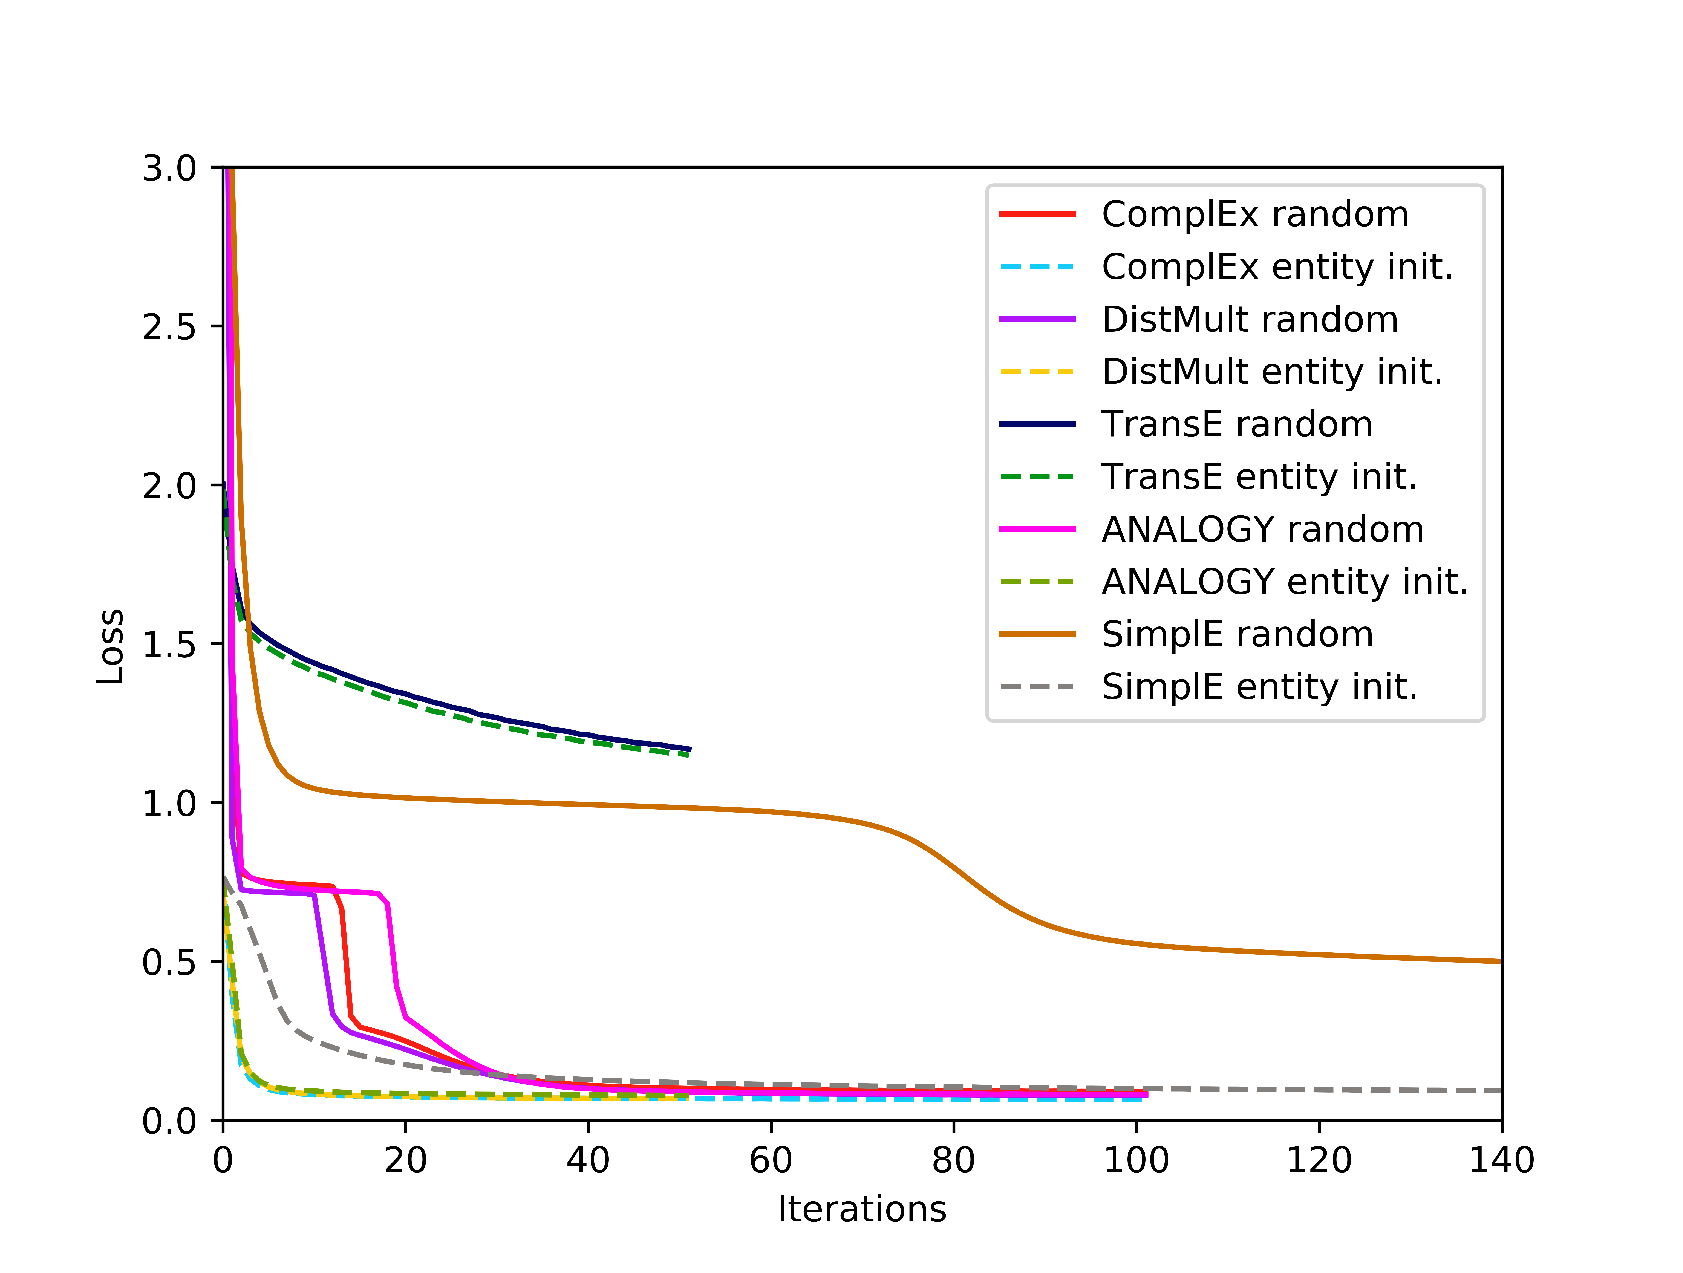
\includegraphics[width=.8\linewidth]{4_kbsintegrationdl/figures/ConvergenceDetail.eps}
    \caption{Loss convergence per iteration for each studied model according to the employed initialization. Dashed lines relate to entity initialization, whereas solid lines represent random initialization.}
    \label{fig:convergence}
\end{figure}


In TransE, no improvement is observed in neither of the studied datasets. This is directly related to the model's conception, as embeddings are generated following a geometrical approach, not considering latent semantics. Therefore, the additional semantic background provided by the initialization is not exploited by the model and is treated equally as randomly valued initialization.

Besides the improvement in terms of metrics, simple entity initialization has a direct benefit in the training of the KGE models, easing their convergence and reducing the number of iterations. Figure \ref{fig:convergence} evidences that simple entity initialization makes KGE models converge to a stable solution faster than those using random initialization. This statement does not hold in the case of TransE, since the convergence rate of both initialization options remains almost identical.

\subsubsection{Semantic-Based Initialization.}

\begin{figure}[t]
    \centering
    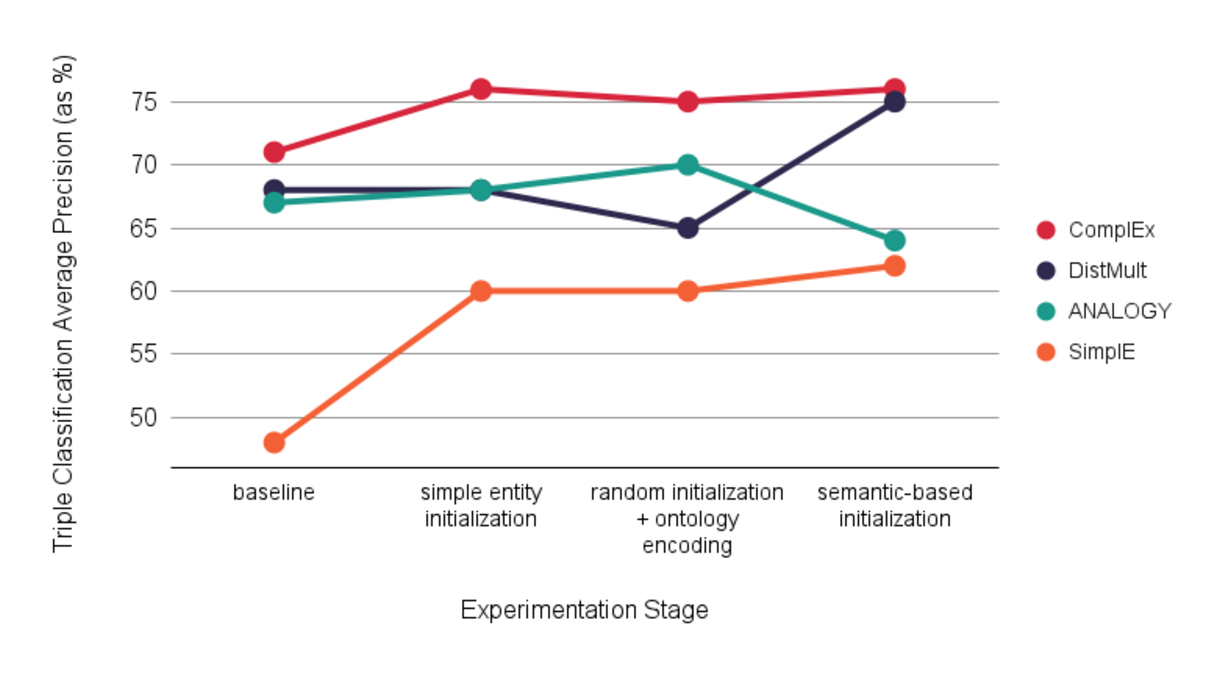
\includegraphics[width=.9\linewidth]{4_kbsintegrationdl/figures/WN_Comparison.eps}
    \caption{WN11 triple classification average precision (in percentage) per model and experimentation stage. Triangle, square, circle and star icons depict the results by ComplEx, DistMult, ANALOGY and SimplE, respectively. }
    \label{fig:wn_stage_comparison}
\end{figure}

According to the results reported in Table \ref{tab:exp_ont_intro}, the application of the complete semantic-based initialization induces an additional improvement over the results achieved with simple entity initialization. In WN11, the results of ComplEx, DistMult and SimplE employing semantic-based initialization noticeably outperform their corresponding baseline models. Figure \ref{fig:wn_stage_comparison} depicts the gradual improvement of each KGE model on WN11. In DistMult, the increment is particularly remarkable, where the baseline model reached a 68\% TCAP, but the introduction of ontological information alongside entity increases this value up to 75\%. The improvement in the case of SimplE is even more noticeable, where the baseline model achieved an accuracy of under 50\%. Semantic-based initialization increases the baseline value in about a 15\%, leading to a total of 62\%. This increment, although less pronounced, is also reflected in ComplEx results. Furthermore, the introduction of ontological information, even with random entity initialization, remarkably improves the baseline models' performance. The simplicity of the employed ontology, comprised of only four disjoint classes, plays a crucial role in this improvement. 

In FB13, although less noticeable, there is still an improvement in several of the reported KGE models. In this scenario, entity initialization does not further enhance the results introduced by adding ontological information to the random initialization. This may be related to the nature of each dataset, as WN11 models semantic relations between words, and can therefore benefit from the inclusion of explicit semantic information. Regarding the ontology choice, it can not be ascertained whether the complexity of the ontology directly impacts the results, as both ontologies produce similar results. Nonetheless, the complexity of the ontology could play a key role in the link prediction task, as it would significantly reduce the dimension of the candidate pool in tasks such as subject or object prediction.


\subsubsection{OOKB Entity Reasoning.}
Once proven that semantic-based initialization enhances the performance of KGE models, the extent of this proposal is evaluated over facts including OOKB entities. As evidenced by the results reported in Table \ref{tab:exp_entity_init}, initializing entities with word embeddings increases the specific knowledge about the entities, providing information that may not be inferred otherwise. Additionally, the inclusion of ontological information improves the generalization aspect of the model, enabling the inference of general restrictions about the relations, which directly translates into an accuracy improvement. Considering these two aspects, the fitness of semantic-based initialization for OOKB entity reasoning is evaluated (Table \ref{tab:OOKB_exp})

\begin{figure}[t!]
    \centering
    \subfigure[FB13 TCAP per relation \label{fig:fb13_tcap}]{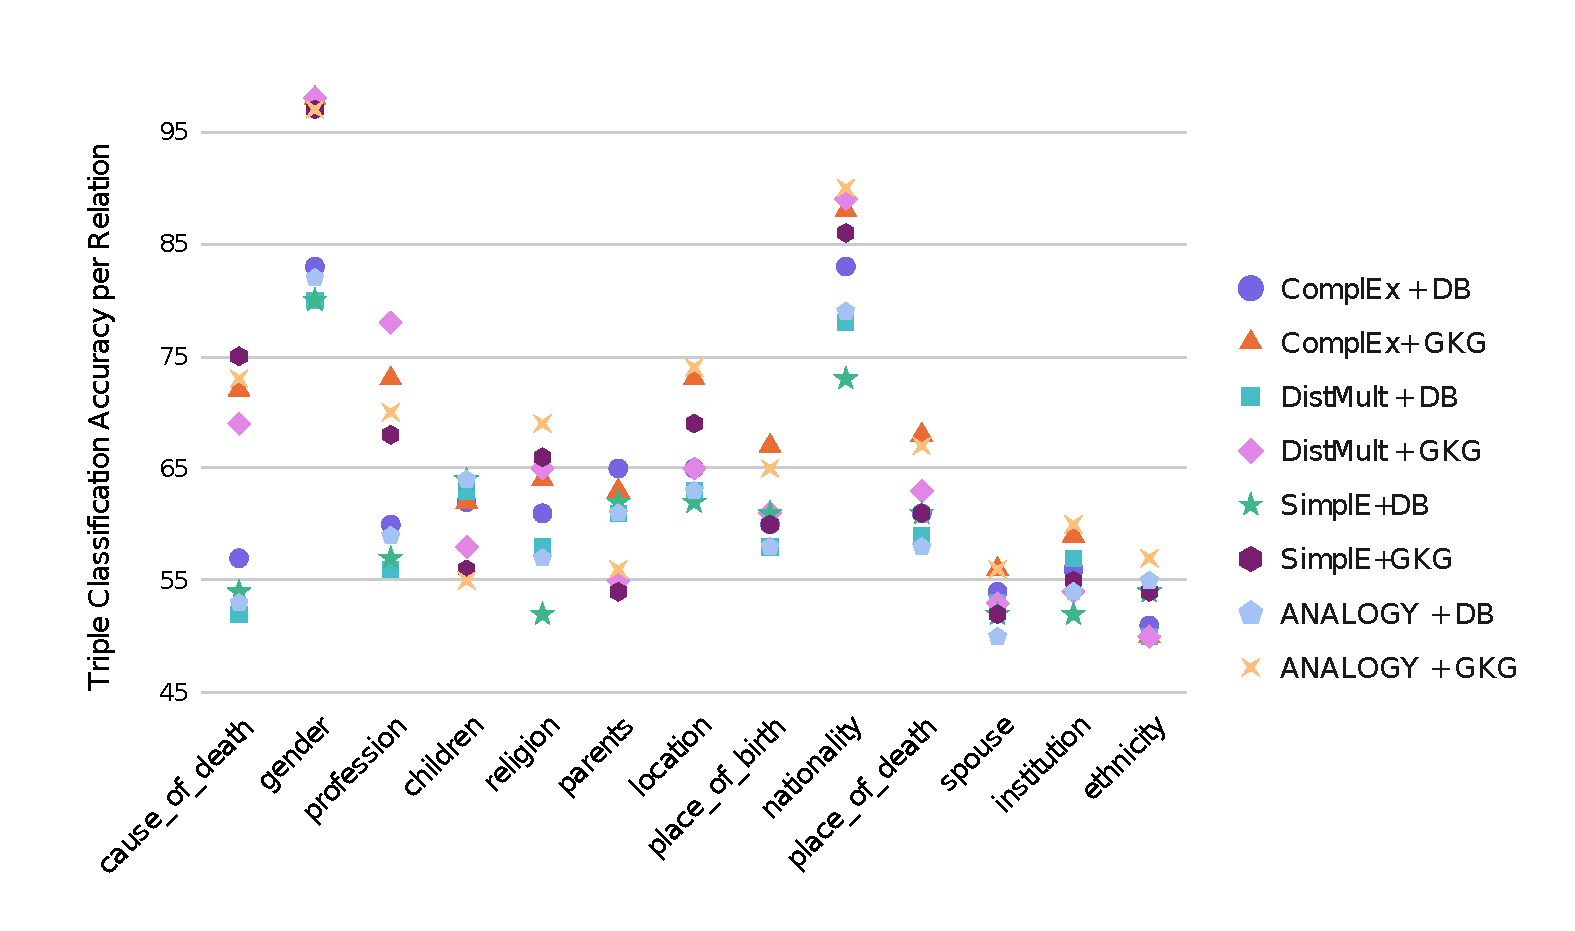
\includegraphics[width=.9\columnwidth]{4_kbsintegrationdl/figures/FB_relation_tcap.eps}}
    \subfigure[WN11 TCAP per relation \label{fig:wn11_tcap}]{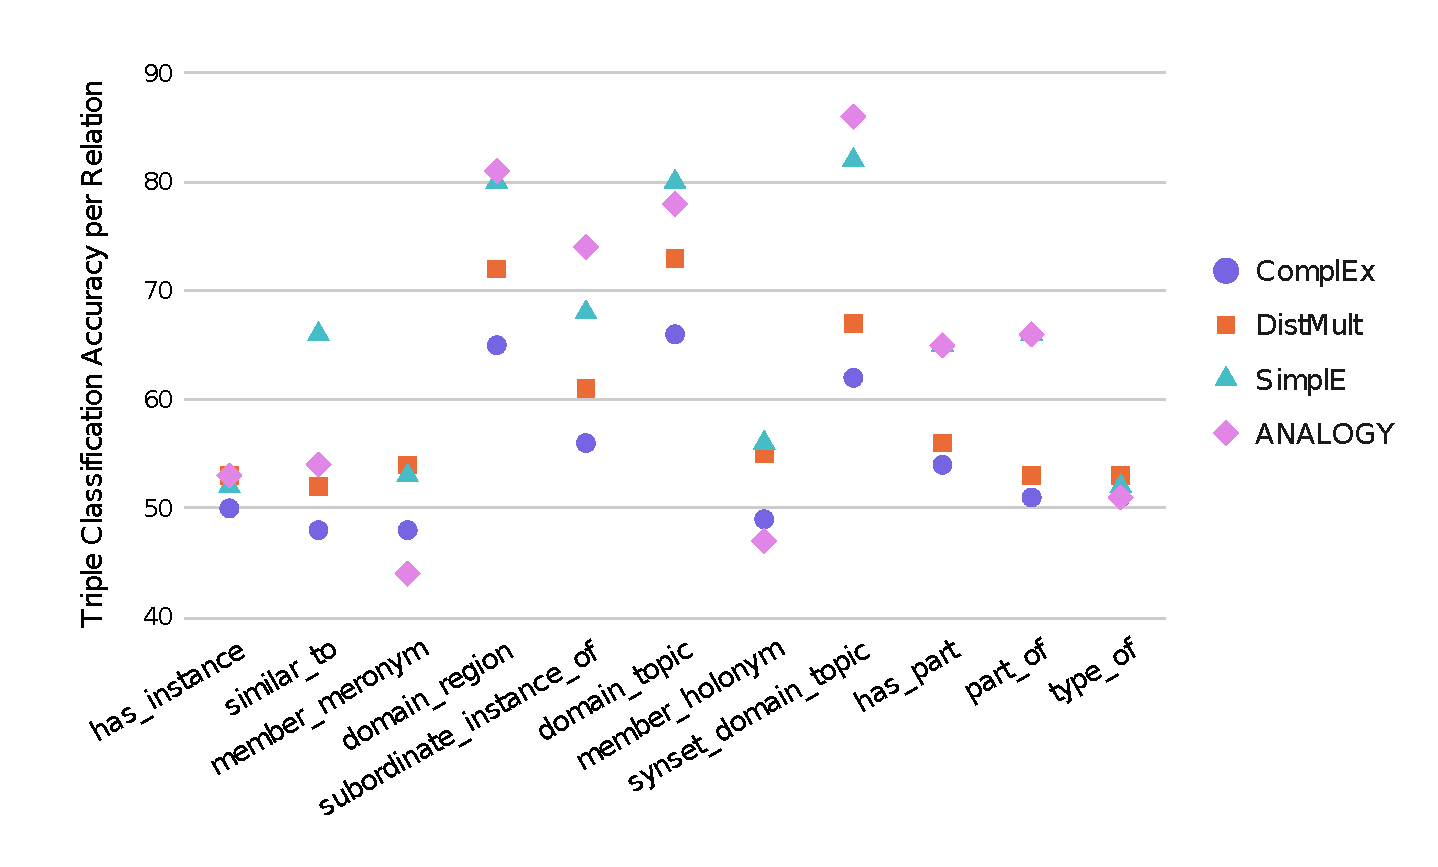
\includegraphics[width=.9\columnwidth]{4_kbsintegrationdl/figures/WN_relation_tcap.eps}}
    \caption{Triple classification average precision (TCAP) in percentage per relation on the OOKB datasets. Figure \ref{fig:fb13_tcap} provides the results on FB13, while Figure \ref{fig:wn11_tcap} illustrates the results obtained in WN11.}
    \label{fig:tcap_OOKB}
\end{figure}

In WN11, while semantic-based initialization considerably enhances the models' performance, no strict class restrictions can be inferred due to the simplicity of the ontology. Therefore, even though the models achieve a high precision over the fully-known test set, this attainment is not extended to the OOKB test set, where the TCAP barely exceeds 50\%. Figure \ref{fig:wn11_tcap} provides an insight on the results obtained by each model on the OOKB test set on each relation. As showcased in the Figure, although the TCAP value ranges between 50\% and 60\% in most relations, it rises to around 70\% in relations such as \textit{domain region} and \textit{domain topic}.

Table \ref{tab:ookb_fb} shows that the results achieved in FB13 for the OOKB test set are similar to those obtained for the fully-known test set, except for DistMult. This phenomenon is related to the type of information modelled in FB13, as the restrictions associated with the relations are closely related to the classes of entities. This statement is further validated by the results in Figure \ref{fig:fb13_tcap}, where the average precision in half of the studied relations reaches more than 70\%. These results show a direct correlation between the homogeneity of the subject and object classes of the relation and the TCAP obtained. Therefore, in relations such as \textit{children}, \textit{parents} or \textit{spouse} that always relate two entities of type \textit{Person}, the precision is always close to 60\% as restrictions are easily inferred. Similarly, the relations \textit{location} and \textit{nationality} also achieve a remarkable performance in terms of precision, even though the results fluctuate across the different models. In both relations, the models employing the GKG ontology achieve better results than those using the DBpedia ontology. This is a direct consequence of the fine-graining level provided by the DBpedia ontology for the general class \textit{Place}, where more than 170 subclasses are identified.

\subsubsection{Performance Analysis.}
%%AQUI VA LO DEL PERFORMANCE ANALYSIS COMO SU NOMBRE INDICA
In addition to improving the transferability, OOKB reasoning via semantic-based initialization can be used to assess the robustness of the KGE model. After evaluating the semantically initialized model on both the fully-known and the OOKB test set, their metrics can be compared. Being $TCAP_{FK}$ and $TCAP_{OOKB}$ the TCAP values of the fully-known and OOKB test sets, respectively, three scenarios can be identified:
\begin{itemize}
    \item \textit{$TCAP_{FK} \gg TCAP_{OOKB}$:} A disparity in favour of the fully-known set can indicate an inapt introduction of ontological information. This induces an exploitative training approach to the KGE model, where the predictions are mainly based on the particularities of the entities. The imbalance in the results may be related to the type of ontological information employed, as well as its complexity. If the KG coverage of the selected ontological information is minimal (i.e., too many rules are selected, or the class hierarchy is too complex), then this can potentially cause a flaw. Simpler ontological information, or a different encoding approach, could solve this imbalance and enhance the generalization capacity of the model. This would result in an improvement of the models' coverage, as well as enabling information sharing between existing and upcoming entities.
    
    \item \textit{$TCAP_{FK} \approx TCAP_{OOKB}$:} A similarity in the results achieved by both sets indicates that the model is appropriately including the ontological information. In this scenario, the KGE model is inferring accurate restrictions about relations, enabling the coverage of OOKB entities. A slight difference in the metrics favouring the fully-known set is expected.
    
    \item \textit{$TCAP_{FK} \ll TCAP_{OOKB}$:} A non-optimal parameter selection can result in an imbalance in favour of the OOKB set. Insufficient learning of specific entity knowledge can result in this result mismatch, indicating that the model has not converged to its optimal solution, but diverged.
\end{itemize}

\subsection{Design Compliance}\label{4_sec:method_assessment}
\begin{figure}[ht]
    \centering
    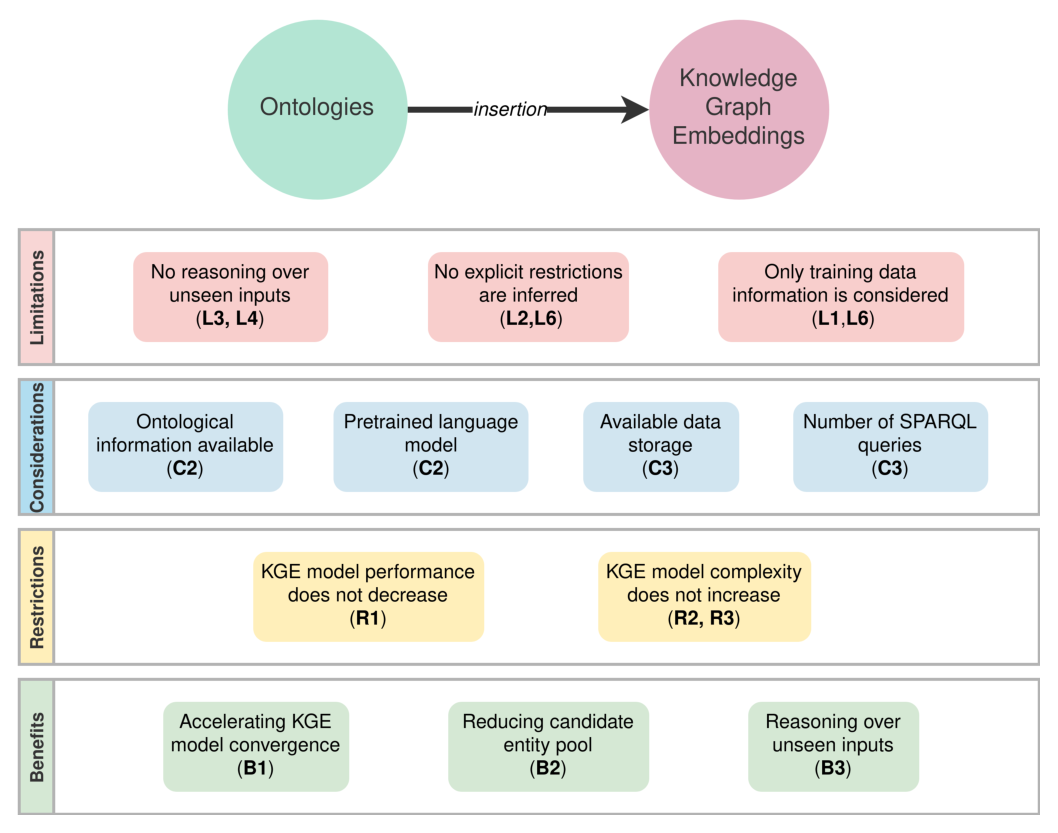
\includegraphics[width=\linewidth]{4_kbsintegrationdl/figures/Instance_KB_into_DL.eps}
    \caption{Method overview on the introduction of ontologies into knowledge graph embedding models. In bold, the general method parameters as depicted in Figure \ref{fig:overview_kbs_dl_intro}.}
    \label{fig:instance_method_kbs_into_dl}
\end{figure}

Semantic-based initialization instantiates the introductory integration method proposed in Section \ref{4_sec:methodology_kbs_intro_dl}. Figure \ref{fig:instance_method_kbs_into_dl} depicts the specific integration parameters of the presented case:

\paragraph{Limitations}
\begin{itemize}
    \item \textbf{No reasoning over unseen inputs.} One of the main challenges regarding KGE models is the codification of unseen elements. KGE models generate representations for the elements existing in a KG during the training time. After training, the representations of each entity and relations are stored in a keyed structure. Hence, if the model is queried for the representation of an unseen element, no representation can be returned as it has no key assigned. Retraining the model from scratch is then needed to generate a feasible representation for unseen elements, limiting its transferability (\ref{kbsintrodl_L_transfer}). While the approaches presented in Section \ref{4_sec:ontointro_kgc} potentially solve this issue, they still require at least a partial retraining. Therefore, the benefit of generating a representation for a single element is severely imbalanced with respect to its computational cost (\ref{kbsintrodl_L_cost}). 
    
    \item \textbf{No explicit restrictions are inferred.} KGE models follow an exploitative training approach. Therefore, the restrictions learned about facts are only based on the training data, which can be subject to errors and lead to inconsistencies (\ref{kbsintrodl_L_constraint}). The constraints learned by the KGE model can therefore be inaccurate and produce different outputs for seemingly similar entities (\ref{kbsintrodl_L_brittleness}).  
    
    \item \textbf{Only training data information is considered.} While there are approaches that extend KGE models with external information, baseline KGE models only consider training data for embedding generation. Using training data as the only source bounds the embeddings to the quality and quantity of the data (\ref{kbsintrodl_L_data_hungry}). Including external data sources could ease the reliance of the model on the training data, as well as potentially enabling the inference of better internal patterns (\ref{kbsintrodl_L_constraint}). 
\end{itemize}
\paragraph{Considerations}
\begin{itemize}
    \item \textbf{Ontological information available.} Ontologies play a fundational role in the generation of KGs, serving as a scaffold for the introduction of new elements. Even though the KG and the ontology are closely related, they may not be always disclosed together. Therefore, while the KG may be publicly available, its ontological information may remain unveiled (\ref{kbsintrodl_C_data}) or may only be accessible via queries.
    
    \item \textbf{Pretrained language model.} The proposed initialization replaces random values with meaningful semantic representations. A pretrained language model is used to generate the initial representations. There is a wide variety of existing models, each trained on their specific corpus and with different embedding dimensions. The selected language model should be aligned with the nature of the knowledge contained in the KG, as well as providing representations of a dimension compatible with the KGE (\ref{kbsintrodl_C_data}).
    
    \item \textbf{Available data storage.} Semantic-based initialization does not require any additional processing resources, such as GPU units. However, it can cause a higher demand on the storage capacity, as it requires the storage of information external to the KG. The data required for initialization is not as sizable at the KG itself, but it is still necessary to ensure that there is enough capacity for its storage (\ref{kbsintrodl_C_resource}).
    
    \item \textbf{Number of SPARQL queries.} In those cases where the ontology files are not available, a SPARQL endpoint may be used to retrieve the required information. For each targeted element in the graph (entities or relations), a SPARQL query may be set to retrieve the specific ontological information. Subsequently, the number of queries grows linearly with the size of the KG. While SPARQL queries have execution times of fractions of a second, if the number of queries to execute is elevated, it can translate into high execution times. Additional, as SPARQL queries are performed online, they are subjected to latency and network failures (\ref{kbsintrodl_C_resource}). 
\end{itemize}
\paragraph{Restrictions}
\begin{itemize}
    \item \textbf{KGE model performance must not decrease.} One of the general restrictions of the proposed method, \ref{kbsintrodl_R_performance} states that to perform KBS introduction, it must be ensured that the performance of the primary DL model will not decrease. This restriction is satisfied in the proposed use case, as none of the studied KGE models experience a decrement on its performance metrics. 
    
    \item \textbf{KGE model complexity does not increase.} The KGE models studied in this use case all have a complexity order of $\mathcal{O}(d)$, where $d$ is the dimension of the embeddings. However, this is  not the case for every KGE model. In Graph Neural Networks, their complexity order is not related to the dimension of the embedding, but to the number of entities and relations in the graph, which can lead to considerably more complex models. Semantic-based initialization is performed offline, thus ensuring that the complexity of the model remains unchanged (\ref{kbsintrodl_R_complexity}). Moreover, as it is performed independently from the KGE model, it does not increase the required training resources (\ref{kbsintrodl_R_resource}).
\end{itemize}
\paragraph{Benefits}
\begin{itemize}
    \item \textbf{Accelerating KGE model convergence.} Figure \ref{fig:convergence} depicts the learning curves of the considered KGE models with and without semantic-based initialization. Even though each pair of models (initialized and non-initialized) are trained for the number of epochs, the difference in their convergence rate is visibly noticeable. Non-initialized models present dramatic changes in the shape of their learning curves, reaching their final inflection point considerably later than their initialized counterparts. The presented use case therefore showcases the fulfilment of benefit \ref{kbsintrodl_B_convergence}.
    
    \item \textbf{Reducing candidate entity pool.} In link prediction, the goal is to find the missing entity of an incomplete fact such that its feasibility is maximized. In the case of subject prediction, given an incomplete fact $(?,p,o)$, each potential fact $(e,p,o)$ $\forall e \in \mathcal{E}$ is computed and rated in decreasing order. The element featured in the top position is outputted by the model as the solution. If explicit restrictions about the subject and object elements featured on each predicate are included in the model, the pool of candidate entities is reduced to those entities in $\mathcal{E}$ that fit the restriction of the relation. Therefore, the computation of feasible triples is reduced to $(e,p,o)$ $\forall e \in \mathcal{E}'$, being $\mathcal{E}'$ the set of entities that fit the relation constraints. This reduces the computation time of the model, which subsequently benefits from the introduction of explicit constraints (\ref{kbsintrodl_B_restrictions}).
    
    \item \textbf{Reasoning over unseen inputs.} One of the main outcomes of the proposed initialization is the induced capacity of KGE models to reason over unseen inputs. Semantic-based initialization enables a descriptive and unique representation of unseen elements without the need of explicitly declaring additional facts or knowledge about them (\ref{kbsintrodl_B_reduce}). However, the level of inference enabled over unseen elements remains superficial and therefore should not be used to directly introduce new facts into the KG. Instead, it can be treated as a filtering element to find potential introduction candidates.
\end{itemize}


\section{Summary}\label{4_sec:summary}
\elvitodo{TBD: Hay que relacionarlo con las contribuciones, objetivos. Lo completaré al terminar la metodología para cuadrarlo.}

%\chapter{Deep Learning Introduction into Knowledge-Based Systems}
\label{chap:dlintegrationkbs} 

This chapter \blfootnote{Amador-Domínguez, E., Serrano, E., Manrique, D., & Bajo, J. (2021). A Case-Based Reasoning Model Powered by Deep Learning for Radiology Report Recommendation. Int. J. Interact. Multim. Artif. Intell., 7(2), 15. doi:10.9781/ijimai.2021.08.011}presents the second insertion integration between deep learning models and knowledge-based systems. Section \ref{5_sec:dl_intro_kbs_methodology} presents the method parameters for the insertion of deep learning models in a knowledge-based system. This insertion method is instantiated into a hybrid framework, combining a case-based reasoning (CBR) model with different deep learning modules. Section \ref{5_sec:dl_powered_kbs_medical} outlines the main features of the proposed framework, focusing on its application in the medical domain. In this context, a CBR powered by DL modules for the generation of medical reports is presented. This scenario showcases the benefits of the introduction of DL into a CBR model, such as enabling reasoning over complex data (i.e., textual reports and images) or enhanced scalability. Section \ref{5_sec:raidologist} instantiates the proposed framework in its use for radiological report generation. Section \ref{5_sec:experimental_results} presents the experimental results. The compliance of the case scenario regarding the general design method is outlined in Section \ref{5_sec:design_compliance}. The chapter is summarized in Section \ref{5_sec:summary}. 


\section{Deep Learning Insertion in Knowledge-Based Systems}\label{5_sec:dl_intro_kbs_methodology}
\begin{figure}[t]
    \centering
    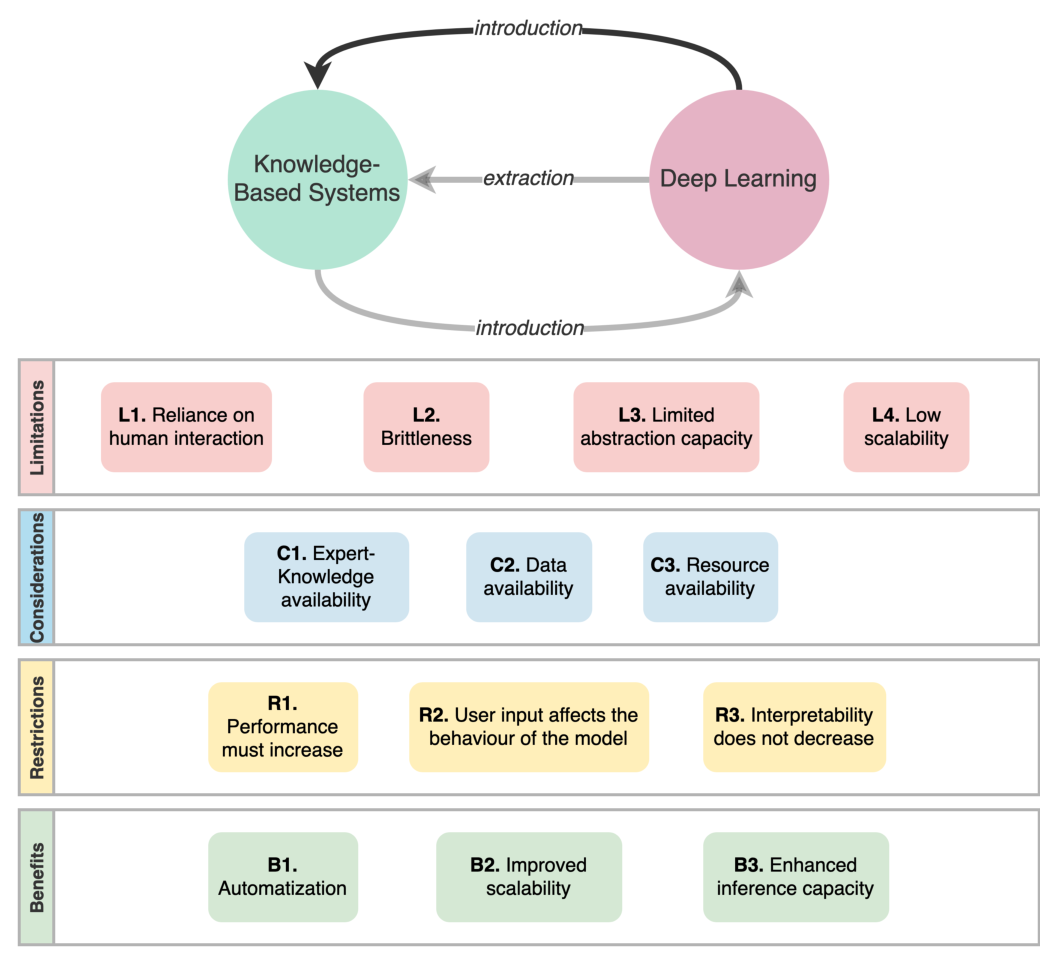
\includegraphics[width=\linewidth]{5_dlintegrationkbs/figures/DL_intro_KBS.eps}
    \caption{Overview on the Insertion of Deep Learning into a Knowledge-Based System.}
    \label{fig:overview_dl_kbs_intro}
\end{figure}
In the second integration approach, the KBS is the primary model, while DL serves as a supporting element. Figure \ref{fig:overview_dl_kbs_intro} outlines the design parameters for the introduction of DL into KBS.
\paragraph{Limitations}
\begin{enumerate} [start=1,label={\bfseries L\arabic*.}]
    \item \textbf{Reliance on human interaction.} \label{dl_intro_kbs_L_human} While some KBS behave autonomously, the majority of them have expert knowledge as their cornerstone.  Expert knowledge can not be automatically elicited, as it comes directly from human users. Moreover, the implication of human users within the KBS may not be only limited to their deployment, but can also be required for validation, extension, and maintenance. 
    \item \textbf{Brittleness.}\label{dl_into_kbs_L_brittle} In DL models, brittleness was a result of the nonexistence of restrictions. In the case of KBS, prediction instability is induced by the use of discrete formalization. These hardcoded generalizations about data hinder the capture of exceptions, making the system volatile to the presence of noise and data changes.  
    \item \textbf{Limited abstraction capacity.}\label{dl_into_kbs_L_abstraction} Most KBS models rely on formal representations to reason over input data. Some of these representations have a probabilistic background (e.g. Bayesian Networks) that enables some degree of uncertainty on the predictions of a given input. However, even probabilistic KBS models experience difficulties when processing inputs that do not fall within the specified representations. Moreover, the number of formalizations required to cover over all the elements in the KB are subject to combinatorial explosions, limiting its reasoning capability.
    \item \textbf{Low scalability.}\label{dl_into_kbs_L_scalability} KBS, specially rule-based models, grow proportionally to the size of the KB. Additionally, generating knowledge bases for KBS is an expensive and tedious process. There are approaches to automatically extract KBs from unstructured data, but they still require expert supervision to ensure the correctness of the mined information. Subsequently, the scalability of KBS is remarkably limited.  
\end{enumerate}

\paragraph{Considerations}
\begin{enumerate} [start=1,label={\bfseries C\arabic*.}]
    \item \textbf{Expert-Knowledge availability}\label{dlintrokbs_C_expert} As outlined in \ref{dl_intro_kbs_L_human}, most KBS rely on expert knowledge for its construction and maintenance. Regardless of whether DL is integrated within the KBS, expert knowledge must be guaranteed before developing the KBS. Moreover, its availability should be extended to the maintenance stage to ensure that the system behaves correctly.
    
    \item \textbf{Data availability}\label{dlintrokbs_C_data} KBS do not require an elevated amount of data. DL models, however are data hungry (as outlined in \ref{kbsintrodl_L_data_hungry} of KBS introduction into DL). Before integrating DL within a KBS model, it must be ensured that enough data for DL model training is available. 
    
    \item \textbf{Resource availability}\label{dlintrokbs_C_resource} Opposite to DL models, KBS do not require powerful computational resources to run. Instead, KBS models need to store the KBs and, in some approaches, the reasoning representations. The integration of KBS and DL in this context poses two challenges, as both storage and computational resources need to be assured for both elements to function.
\end{enumerate}
\paragraph{Restrictions}
\begin{enumerate} [start=1,label={\bfseries R\arabic*.}]
    \item \textbf{Performance must increase.} \label{dlinstrokbs_R_performance} The inclusion of DL in a KBS carries an computational cost. Therefore, the resulting hybrid approach is expected to show a performance improvement with respect to the baseline KBS for the integration to be cost-effective. 
    
    \item \textbf{User input affects the behaviour of the model.}\label{dlintrokbs_R_user} User input is indispensable for KBS models (\ref{dl_intro_kbs_L_human}). While it can be perceived as limiting, it ensures the correct behaviour of the KBS. The impact that external input has on the behaviour of the system should remain with the introduction of DL, correcting not only the behaviour of the KBS but also of the DL.
    
    \item \textbf{Interpretability does not decrease.}\label{dlintrokbs_LR_interpretability} One of the main assets of KBS is their high interpretability. KBS are designed to both integrate external input and produce outputs whose inference process can be understood by humans. DL models, on the contrary, behave as black-boxes. Therefore, their integration should be performed in a way that does not obscure the inference process, so that it can still be understandable.
    
\end{enumerate}
\paragraph{Benefits}
\begin{enumerate} [start=1,label={\bfseries B\arabic*.}]
    \item \textbf{Automatization.}\label{dlintrokbs_B_automatization} As outlined in \ref{dl_intro_kbs_L_human}, human interaction (specially expert knowledge) is essential for generating and maintaining KBS. DL models, on the contrary, have a mostly autonomous behaviour. Therefore, the introduction of DL in KBS may serve to automatize some of the steps required to deploy, maintain and validate KBS, reducing the need of human intervention.
    
    \item \textbf{Improved scalability.}\label{dlintrokbs_B_scalability} KBS are limited in terms of scalability due to their reliance on human intervention (\ref{dl_into_kbs_L_scalability}). The inclusion of DL modules within the KBS, as well as automatizing some tasks, can improve the scalability of the system. For example, extracting formal representations from a set of unstructured data.
    
    \item \textbf{Enhanced inference capacity.}\label{dlintrokbs_B_inference} KBS models struggle with capturing non explicit exceptions from data (\ref{dl_into_kbs_L_brittle}. DL models infer abstract patterns from data, capable of assigning an output for any input, even for outliers. Moreover, DL models only require samples of previously unseen inputs to infer new feasible patterns for their correct classification (\ref{dl_into_kbs_L_abstraction}). The introduction of DL modules into a KBS could not only enhance its abstraction capacity, but improving the reasoning of the model on outlier elements.

\end{enumerate}


\section{Deep Learning Powered Case-Based Reasoning for Medical Document Processing}\label{5_sec:dl_powered_kbs_medical}
Case-Based Reasoning (CBR) integration with DL is one of the scenarios depicted in Section \ref{sec:sota_dl_kb_intregration}. As denoted, CBR is often posed as an alternative to rule-based systems. This Section presents a use case on the medical domain, where DL modules are injected into a CBR model. One of the most interesting conclusions of the systematic review in \cite{amador_systematic_review_2019} is the predominance of interpretable, knowledge-based systems in the medical domain. Explainability was rated as one of the key features of these models, thus showing its relevance for its application to this domain. Therefore, the CBR acts as the primary model in this scenario, ensuring that the final hybrid DL-powered approach remains interpretable. 

\begin{figure}[t]
    \centering
    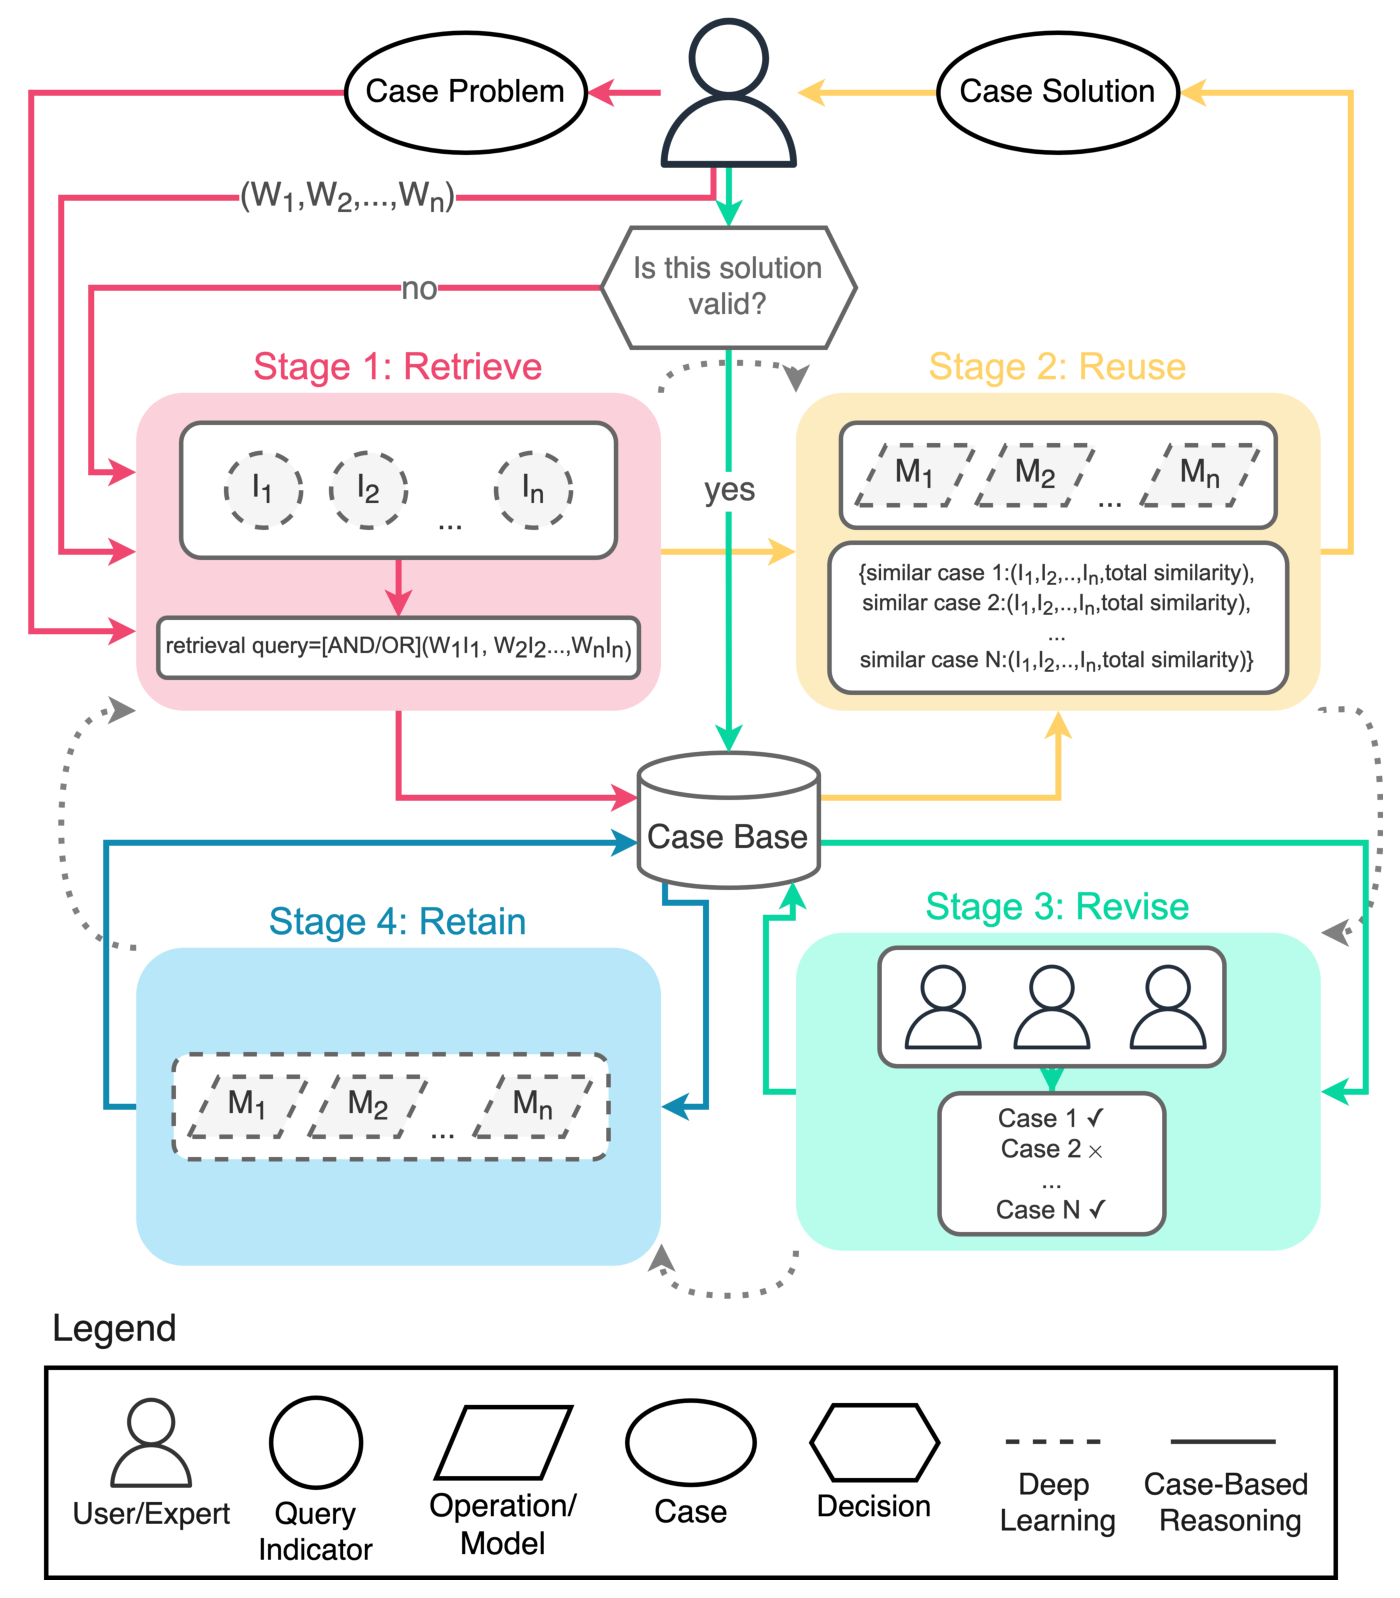
\includegraphics[width=.8\linewidth]{5_dlintegrationkbs/figures/Overview_CBR_DL.eps}
    \caption{Overview of the Deep Learning powered Case-Based Reasoning Model.}
    \label{fig:overview_CBR_DL}
\end{figure}

Figure \ref{fig:overview_CBR_DL} depicts a general overview of the proposed hybrid model. Dashed line denotes the elements where DL can be introduced so that the integrity and interpretability of the CBR model is not compromised, but a performance enhancement is induced. The proposed framework provides assistance in the generation of medical reports, as presented in \cite{DBLP:journals/ijimai/Amador-Dominguez21}. It is not devised to replace the behaviour of the expert, but to provide formal corrections, references, and suggestions to improve the final quality of the results. 

CBR behaves cyclically, comprising four stages: retrieve, reuse, revise, and retain \citep{overview_cbr}. These stages are differentiated in Figure \ref{fig:overview_CBR_DL}, showing the interactions between phases, as well as between the framework and the user. 

\color{purple}

\paragraph{Retrieve}\label{5_sec:dl_powered_cbr_retrieve}
The CBR cycle is initiated when the user inputs a new case problem. A case problem can be simply a text draft, or it can include additional relevant information such as images, related terms or references. In the first stage of the CBR cycle, retrieve, the goal is to determine which of the cases stored in the case base have a higher resemblance to the input. A naïve approach to find the existing closest cases is to use a simple \textit{K-Nearest Neighbours} (K-NN) algorithm, where $K$ is the number of cases to retrieve and the selection is purely based on the distance between the input and the existing samples. K-NN offers a straightforward and efficient solution, but it exhibits two shortcomings that hinder its usage: i) the input data may not always be numerical and easy to measure, and ii) the application domain is expert-oriented, so more specific and revised criteria are required to accurately retrieve cases.

While similarity between reports can be measured according to quantitative metrics such as the age of the patient or demographic data, there are no fixed static criteria that enable straightforward comparison. Some metrics may remain static between comparisons, but others may vary between users. The proposed framework uses an indicator-based retrieval algorithm to overcome these issues. Instead of comparing the cases as a whole, the retrieval algorithm evaluates the values of the different indicators for each case. As depicted in Figure \ref{fig:overview_CBR_DL}, the number of indicators is not predefined and can be adapted to fit different case scenarios. For its application in the medical domain, four indicators are identified:
\begin{itemize}
    \item I1. \textit{Image Comparison.} Images are the cornerstone of some medical areas, such as neurology or dermatology. In those fields where pictures provide essential information, they should not be diluted within the text, but treated separately. Several methods for image comparison can be considered, ranging from histogram to feature vector comparison. Convolutional Neural Networks (CNNs) are a potential DL option for this indicator. CNNs are possibly the most robust way to translate images into a fixed-dimensional space. However, simpler, non-DL alternatives can be also applied. Feature matching algorithms, such as SURF \citep{image_surf}, ORB \citep{ORB_image} or KAZE \citep{KAZE_images} are potential interpretable alternatives to CNNs. However, feature matching algorithms are highly sensitive to potential image failures, such as light flashing, and cannot capture finer-grained information. A potential solution for this issue is to combine differently generated vector representations into a unique vector. Once the image is embedded into a single vector, distance-based can be performed to measure the similarity with respect to the existing images.
    
    \item I2. \textit{Document Comparison.} Similar to the previous case, multiple approaches can be considered for document comparison. Non-feature-based methods can perform this task, but their performance is noticeably subpar with respect to that where documents are embedded into a vector space and can be compared using distance-based metrics. Language models such as ELMO (Embeddings for Language Models) \citep{elmo} or BERT (Bidirectional Encoder Representations for Transformers) \citep{bert} are the preferred choices for document embedding, but simpler methods such as bag-of-words or TF-IDF can also be applied. Despite reducing the computational cost, these methods cannot capture the underlying semantic information, which leads to less expressive representations. Regarding embedding comparison, different paradigms can be considered, depending both on the type of documents to compare and their purpose. In this respect, cosine similarity, word's mover distance \citep{word_mover_distance}, or probabilistic based methods (in which the embedding is converted into a probabilistic distribution) are suitable choices.
    
    \item I3. \textit{Named Entity Comparison.} Named Entity Recognition (NER) is one of the key tasks in the Natural Language Processing area, being particularly relevant in the medical domain. The goal of this task is to detect and label relevant terms within the text, such as people, places, or dates. Its use is particularly extended in the medical domain, where several NER models have been developed to identify specific medical terms within texts such as diseases, proteins or drugs. CliNER \cite{cliner}, BioBERT \citep{biobert} or SciBERT \citep{scibert} are examples of clinical NER models. Annotating relevant terms within documents can be an effective tool to detect and retrieve related documents. Therefore, only those cases whose reports contain relevant terms are considered for retrieval, greatly reducing the search scope.
    
    \item I4. \textit{Noise Filtering Criteria.} Additional filtering criteria to discard unfitting cases may be required in addition to the previous indicators. These criteria focus on formatting specifications (i.e. absence of images, language) or content elements (i.e. typos, number of abbreviations unidentified). Filtering criteria can be customized to be as restrictive as necessary. 
\end{itemize}

For each indicator, the user can establish a threshold value. Indicators can be treated either conjunctively or disjunctively, according to the user's preference. These criteria are then translated into a search query, which is executed to retrieve the specified number of cases which meet the user-provided constraints.

\begin{lstlisting}[captionpos=b, breaklines=true, float=tp,floatplacement=tbp, caption=Example of a retrieval query., label=lst:lst_query_sample,basicstyle=\ttfamily,frame=single]
   query={ I1>=0.85, I2>=0.7, I3=[Pulmonary Disease,  Pneumonia], I4=[lang= 'en', identified_abbrv_rate>= 0.9 ], N=5, operation= 'OR'}
\end{lstlisting}

Listing \ref{lst:lst_query_sample} is an example of a retrieval query. This query specifies the retrieval of the top 5 cases that either:
\begin{itemize}
    \item Include images that are similar to at least 85\% to those present in the input report.
    \item Medical reports are similar in at least 70\%.
    \item Contain medical terms \textit{pulmonary disease} and \textit{pneumonia}.
    \item Are written in English, and at least 90\% of the detected abbreviations have been disambiguated.
\end{itemize}

Cases that meet the retrieval criteria are ordered in descending order according to their cumulative similarity across the indicators. The top \textit{k} cases demanded by the user are returned.

\paragraph{Reuse}\label{5_sec:dl_powered_cbr_reuse}
As depicted in Figure \ref{fig:overview_CBR_DL}, the reuse stage starts once the top \textit{k} similar cases are retrieved. A brief summary on the results of the indicators of each selected case is provided to the user to keep the transparency of the model. From the instances retrieved in the previous stage, different operations are performed to obtain helpful, relevant information to assist the user in the generation of the report. Different modules perform several operations, as depicted in Figure \ref{fig:overview_CBR_DL}. As denoted by the dashed line, these modules can be implemented using DL. In the present case scenario, four modules are identified:
\begin{itemize}
    \item M1. \textit{Formatting Module.} Readability is one of the most prominent features of any written document. Syntactic cohesion, as well as correct formatting are some of the elements that make a document readable. In the case of medical documents, while there may exist differences between specialities, there is usually a fixed structure in which the data is presented. From a general standpoint, a medical report comprises four main sections:
    \begin{itemize}
        \item \textit{Indication.} A brief introduction to the report, giving superficial information about the patient and the observed symptoms.
        \item \textit{Comparison.} References to previous reports of the same patient.
        \item \textit{Findings.} Extensive information about the potential causes of the symptoms, as well as additional observations about the patient.
        \item \textit{Impression.} Conclusions and diagnosis.
    \end{itemize}
    Therefore, this module generates a structured, paragraphed version of an input report in raw format.
    
    \item M2. \textit{Scoring Module.} The system provides the user a validity score indicating whether the report, in its current form, is readable and understandable. This score can be either a simple binary value (valid or nonvalid), a star-score method, or a finer decimal score.
    
    \item M3. \textit{Disambiguation Module.} Abbreviations are recurrent in the medical domain due to the existence of a considerable number of complex compound terms. While most of these abbreviations may be universal and understandable by any professional, some can still be non-understandable for a regular reader. Therefore, the goal of this module is to detect the existing abbreviations within the text and offer disambiguations for them. While this may increase the extension of the document, it also improves its readability noticeably.
    
    \item M4. \textit{Term Recommendation Module.} As previously stated, NER is a critical challenge in the medical domain. NER models can accurately detect relevant terms in a text and groupd them in a fixed set of categories. These categories are usually related and, subsequently, the corresponding terms. For example, given a report about a patient with a pulmonary disease, terms such as (\textit{pneumonia,disease}) and \textit{(chest x-ray,test)} may be frequently featured together. This module mines these correlations between terms, and suggests their inclusion to the user. NER is performed over the output cases of the retrieval phase, obtaining a set of categorized terms. This set of terms is then flattened, cleaned and presented to the user. In the aforementioned example, if the user is writing a report containing the term \textit{pneumonia}, but not \textit{chest x-ray}, the system may suggest the inclusion of this term due to its existent correlation.

\end{itemize}

As users play a key role in CBR models, the recommendations and suggestions offered by the framework are not final. Instead, the user decides which of the suggestions and corrections are to be applied to the input report. When the user approves the final state of the report, a new case is generated and stored in the case base, using the initial report as the problem and its corrected version as the solution. Case bases are not immediately incorporated into the case base, but marked as \textit{to be validated} until an expert validates them.

\paragraph{Revise}\label{5_sec:dl_powered_cbr_revise}
A new case is generated once the user effectuates the applicable suggestions to the report. New cases are not automatically included in the case base for future iterations of the cycle, as they may include errors that can negatively affect the behaviour of the system. Moreover, if the system stores unreliable cases into the case base without any revision, they may be retrieved in the subsequent iterations, generating erroneous suggestions and corrections. An intermediate step is required to ensure that all cases stored in the case base are useful and relevant. 

In the revise stage, a panel of experts manually checks the upcoming cases, rating and correcting them. The scores provided by the experts must be coherent with the grading system used by the scoring module. Therefore, if the scoring module uses binary scoring, experts must extend this criterium to new cases.


\paragraph{Retain}\label{5_sec:dl_powered_cbr_retain}
One of the main challenges of CBR systems is how to efficiently manage the case base. Ideally, the case base should be optimized, containing the minimum number of relevant cases that ensure the maximum coverage. Non-valid cases are not stored in the case base, but are stored separately to serve as negative samples for the scoring module. 

New cases are being regularly introduced into the case base, subsequently unchaining a reaction within the system. CBR models improve with the inclusion of new cases, which keeps them usable and updated throughout time. In the retain stage of the cycle, besides performing case base maintenance, reuse models are updated and checked. Reuse model updates can be either a replacement for the modules, such as switching from regular expression or rule-based systems (when the number of cases is limited) to DL models when the available data increases. 

\subsection{A Hybrid Case-Based Reasoning and Deep Learning Framework for Radiological Report Recommendation}\label{5_sec:raidologist}

This Section presents an implementation of the general framework depicted in Figure \ref{fig:overview_CBR_DL} focusing specifically on radiological reports. This context presents a challenging scenario, as both image and textual information are equally relevant. Figure \ref{fig:raidologist_data_flow} showcases the data flow of the implementation, instantiating the different components described in Section \ref{5_sec:dl_powered_kbs_medical}. The execution steps of one full iteration of the cycle are also denoted.

\begin{figure}[t]
    \centering
    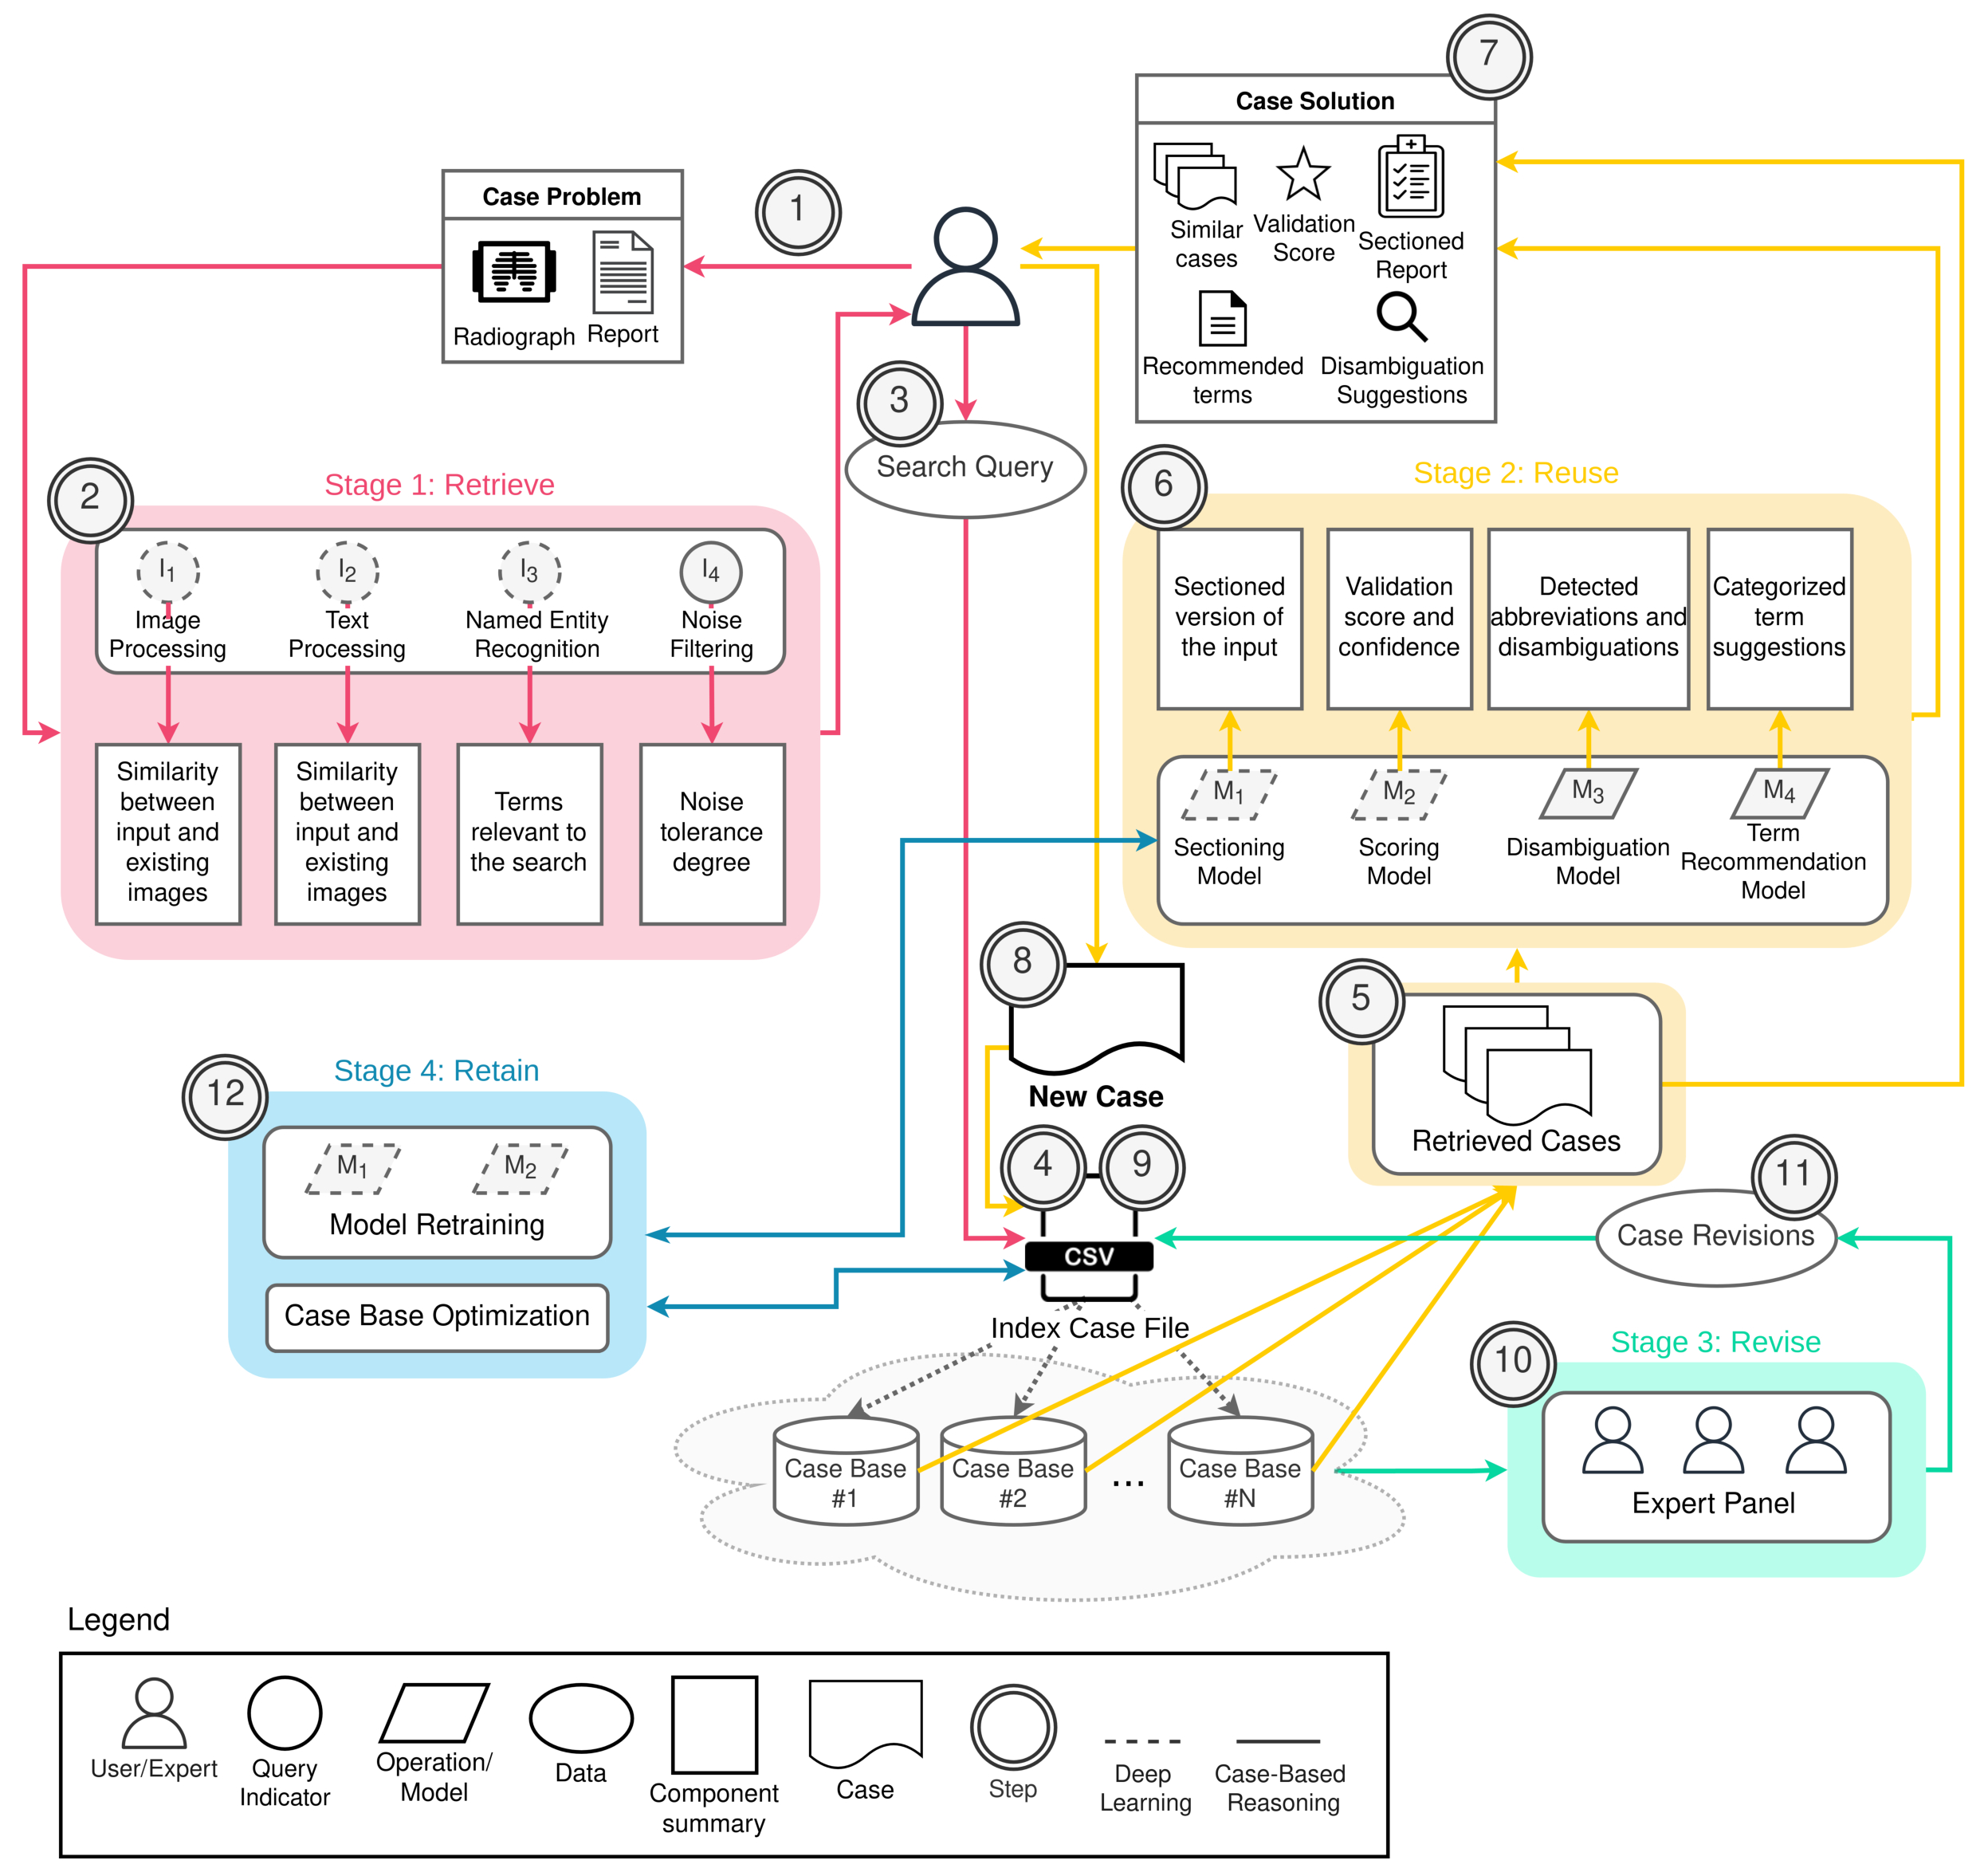
\includegraphics[width=\linewidth]{5_dlintegrationkbs/figures/raidologist_flow.eps}
    \caption{Data flow of the r.AID.ologist framework.}
    \label{fig:raidologist_data_flow}
\end{figure}

The framework is implemented as a four-layered software architecture. Some issues must be addressed before defining the specific components of the proposed hybrid model for the given task, such as data management or storage mechanisms. Indexed storage is employed to deal to efficiently manage the constant growth of the case base while still allowing for efficient retrieval. In the proposed storage, cases are saved either in a distributed or centralized schema and referenced in an index file. The index file contains each case's location and its respective indicators which are computed beforehand, accelerating the retrieval process. 

In the radiology domain, a case is usually composed by one or more radiographs and a brief text summarizing the most relevant findings on the images, alongside additional information about the patient. These are the two minimal elements required to define a case, but additional information can be provided, such as relevant terms, regions of interest, or specific abbreviations. 

The retrieve stage begins when the user inputs a new problem into the system. The case indicators of the input problem are computed as follows:

\begin{itemize}
    \item I1. \textit{Image Comparison.} In radiology, images are black and white radiographs, thus not exhibiting much variation between samples. Convolutional neural networks generate embeddings capable of capturing the subtle differences between radiographs, enabling an accurate comparison between them. A feature detection algorithm is also included to add an additional level of information. KAZE is used to generate fixed-dimension descriptors from a set of key points detected in the image. Key points can be indicated on the image, providing a visualization on the basis on which the images are compared. Both KAZE and CNN vectors are averaged, generating a unique embedding that combines both interpretable and abstract knowledge. Samples are compared via cosine similarity over the resulting embedding.
    
    \item I2. \textit{Report Comparison.} A clinical NLP model is used for this task. This pretrained DL model provides embeddings at word, sentence, and document level. Document embeddings are used to generate comparable report representations. 
    
    \item I3. \textit{Named Entity Recognition} CliNER is used to compute this indicator. CliNER provides a series of models (Bi-Directional Long Short Term Memory networks) trained over a sizeable clinical corpus, capable of identifying the following entity categories: diseases, treatments, and tests. While simple, this categorization is enough to cover the terms identified in the radiology domain.
    
    \item I4. \textit{Noise Filtering.} The same NLP model from I2 is used for noise filtering. In this context, noise encompasses those tokens in the text that cannot be identified as words. Once the report is processed by the NLP model, a set of conflicting terms is obtained. Noise can then be computed as the proportion of identified tokens with respect to the total number of tokens in the text.
\end{itemize}

These indicators are computed only once per case. The user is then inquired for the retrieval query parameters: threshold values of each indicator, the combination paradigm (conjunctive or disjunctive), and the number of cases $k$ to retrieve. The threshold values are reformulated in a human-readable format, as depicted in Figure \ref{fig:raidologist_data_flow}. For example, a valid inquiry for the value of I2 (report comparison) would be: \textit{what is the minimum similarity acceptable between the current and the existing reports?}. Queries must be clearly presented and understandable to the user, as they condition the behaviour of the model during the retrieve phase.

After the search query is generated by the user, a comparison between the current problem and the existing cases is performed. The use of indexed storage enables a fast comparison, as the indicator values of the cases contained in the index file can be directly compared to those of the input. Therefore, a case is only fully retrieved from the case base if it meets the query conditions. A summary of each indicator's similarity metrics is included along each case. 

In the reuse phase, a tailored solution for the input case problem is generated based on the retrieved cases, alongside with the described formatting modules. The retrieved top $k$ similar cases are also included as part of the case solution, serving as format and content references for potential corrections. The devised case solution contains the following suggestions, which are provided to the user:
\begin{itemize}
    \item \textit{Sectioned version of the report:} A DL model (Bi-Directional Long Short Term Memory) is used for text formatting. Sectioning is treated as a classification problem. Training reports are divided into sentences, and each sentence is labelled according to the section where it is featured. Subsequently, the goal of the model is to predict the section where each sentence fits best. When formatting a new report, sentences are input into the DL model in the same order as they appear in the text to avoid content permutations.
    
    \item \textit{Potential disambiguations for text abbreviations:} After computing indicator I4, a list of unidentified tokens is obtained. This set not only comprises noisy entries, such as misspellings, but also abbreviated terms. These tokens are then consulted in the medical terminology SNOMED-CT, seeking to obtain the best applicable term whenever possible.
    
    \item \textit{Case validation score and confidence value:} A binary scoring system is employed to categorize cases between valid and invalid. A DL model composed by a language modelling model in combination with a random forest classifier is used to score the cases, using the cases already validated by the experts in the revise section as training data. While the score assigned to a given case is not final until it has been revised by the experts, it can provide a reference to the user on whether the report on its current state would be suitable for approval. 
    
    \item \textit{Suggested related terms per category:} CliNER is applied to the content of the top $k$ retrieved cases, extracting a set of terms categorized into three types: disease, test, and treatment. Duplicate entries are removed, and the resulting categorized term list is presented to the user.
\end{itemize}

The case solution generated after the reuse phase is then presented to the user, who decides which of the offered corrections should be implemented. A new case is then generated from the initial problem and the solution implemented by the user with the suggestions of the system. This case will then be stored in a case base and labelled as \textit{to be validated} until the revise phase. Non validated cases are not displayed to the user nor used for reuse until their validation by the expert panel. In the revise phase, the expert panel periodically validates the pending cases. The final validation state of new cases is referenced in the index file, accelerating the posterior retrieval search. 

Usually, invalid cases are deleted from the case base, as they technically do not provide valuable information to the user. However, due to the inclusion of DL models, negative samples are necessary to train and obtain robust scoring models. Moreover, once the scoring model reaches enough maturity, it can replace the expert panel, automatizing this phase. 

The retain stage is triggered under one of the following three conditions: i) the expert panel requires it, ii) it is periodically scheduled, or iii) the number of stored cases reaches an specified number. In this stage, both the scoring and sectioning modules used in the reuse stage are updated with the newly added cases. Periodically scheduled retraining ensures that the model is kept updated, but may be ineffective when the number of cases in the case set is reduced. Case based optimization is also performed in this phase. Case correlation is maximized for optimization to obtain the minimum set of cases that give the maximum coverage. First, a global linking process is conducted amongst cases, computing the top 5 similar cases per instance. Cases that are co-referenced by at least one case are kept in the case base. Unreferenced cases are still considered for training the sectioning and scoring models, but will not be part of the CBR cycle in subsequent iterations.


\subsection{Experimental Results}\label{5_sec:experimental_results}
The presented implementation of the proposed hybrid model is evaluated to assess its accuracy and performance. Most CBR-based approaches are gauged focusing on their retrieval strategy. The proposed framework relies on user-input queries to refine the retrieval process. Hence, assessing the performance of the proposal based solely on the effectiveness of the retrieval mechanism would not be representative enough, as the success of this stage is highly reliant on user criteria.

Since the implementation context (radiological domain) is highly expert-oriented, accurately evaluating the framework without expert information is not trivial. An alternative evaluation approach capable of quantitatively measuring the performance of the model is devised. Report correction is used to measure the effectiveness of the proposal.

\begin{figure}[t]
    \centering
    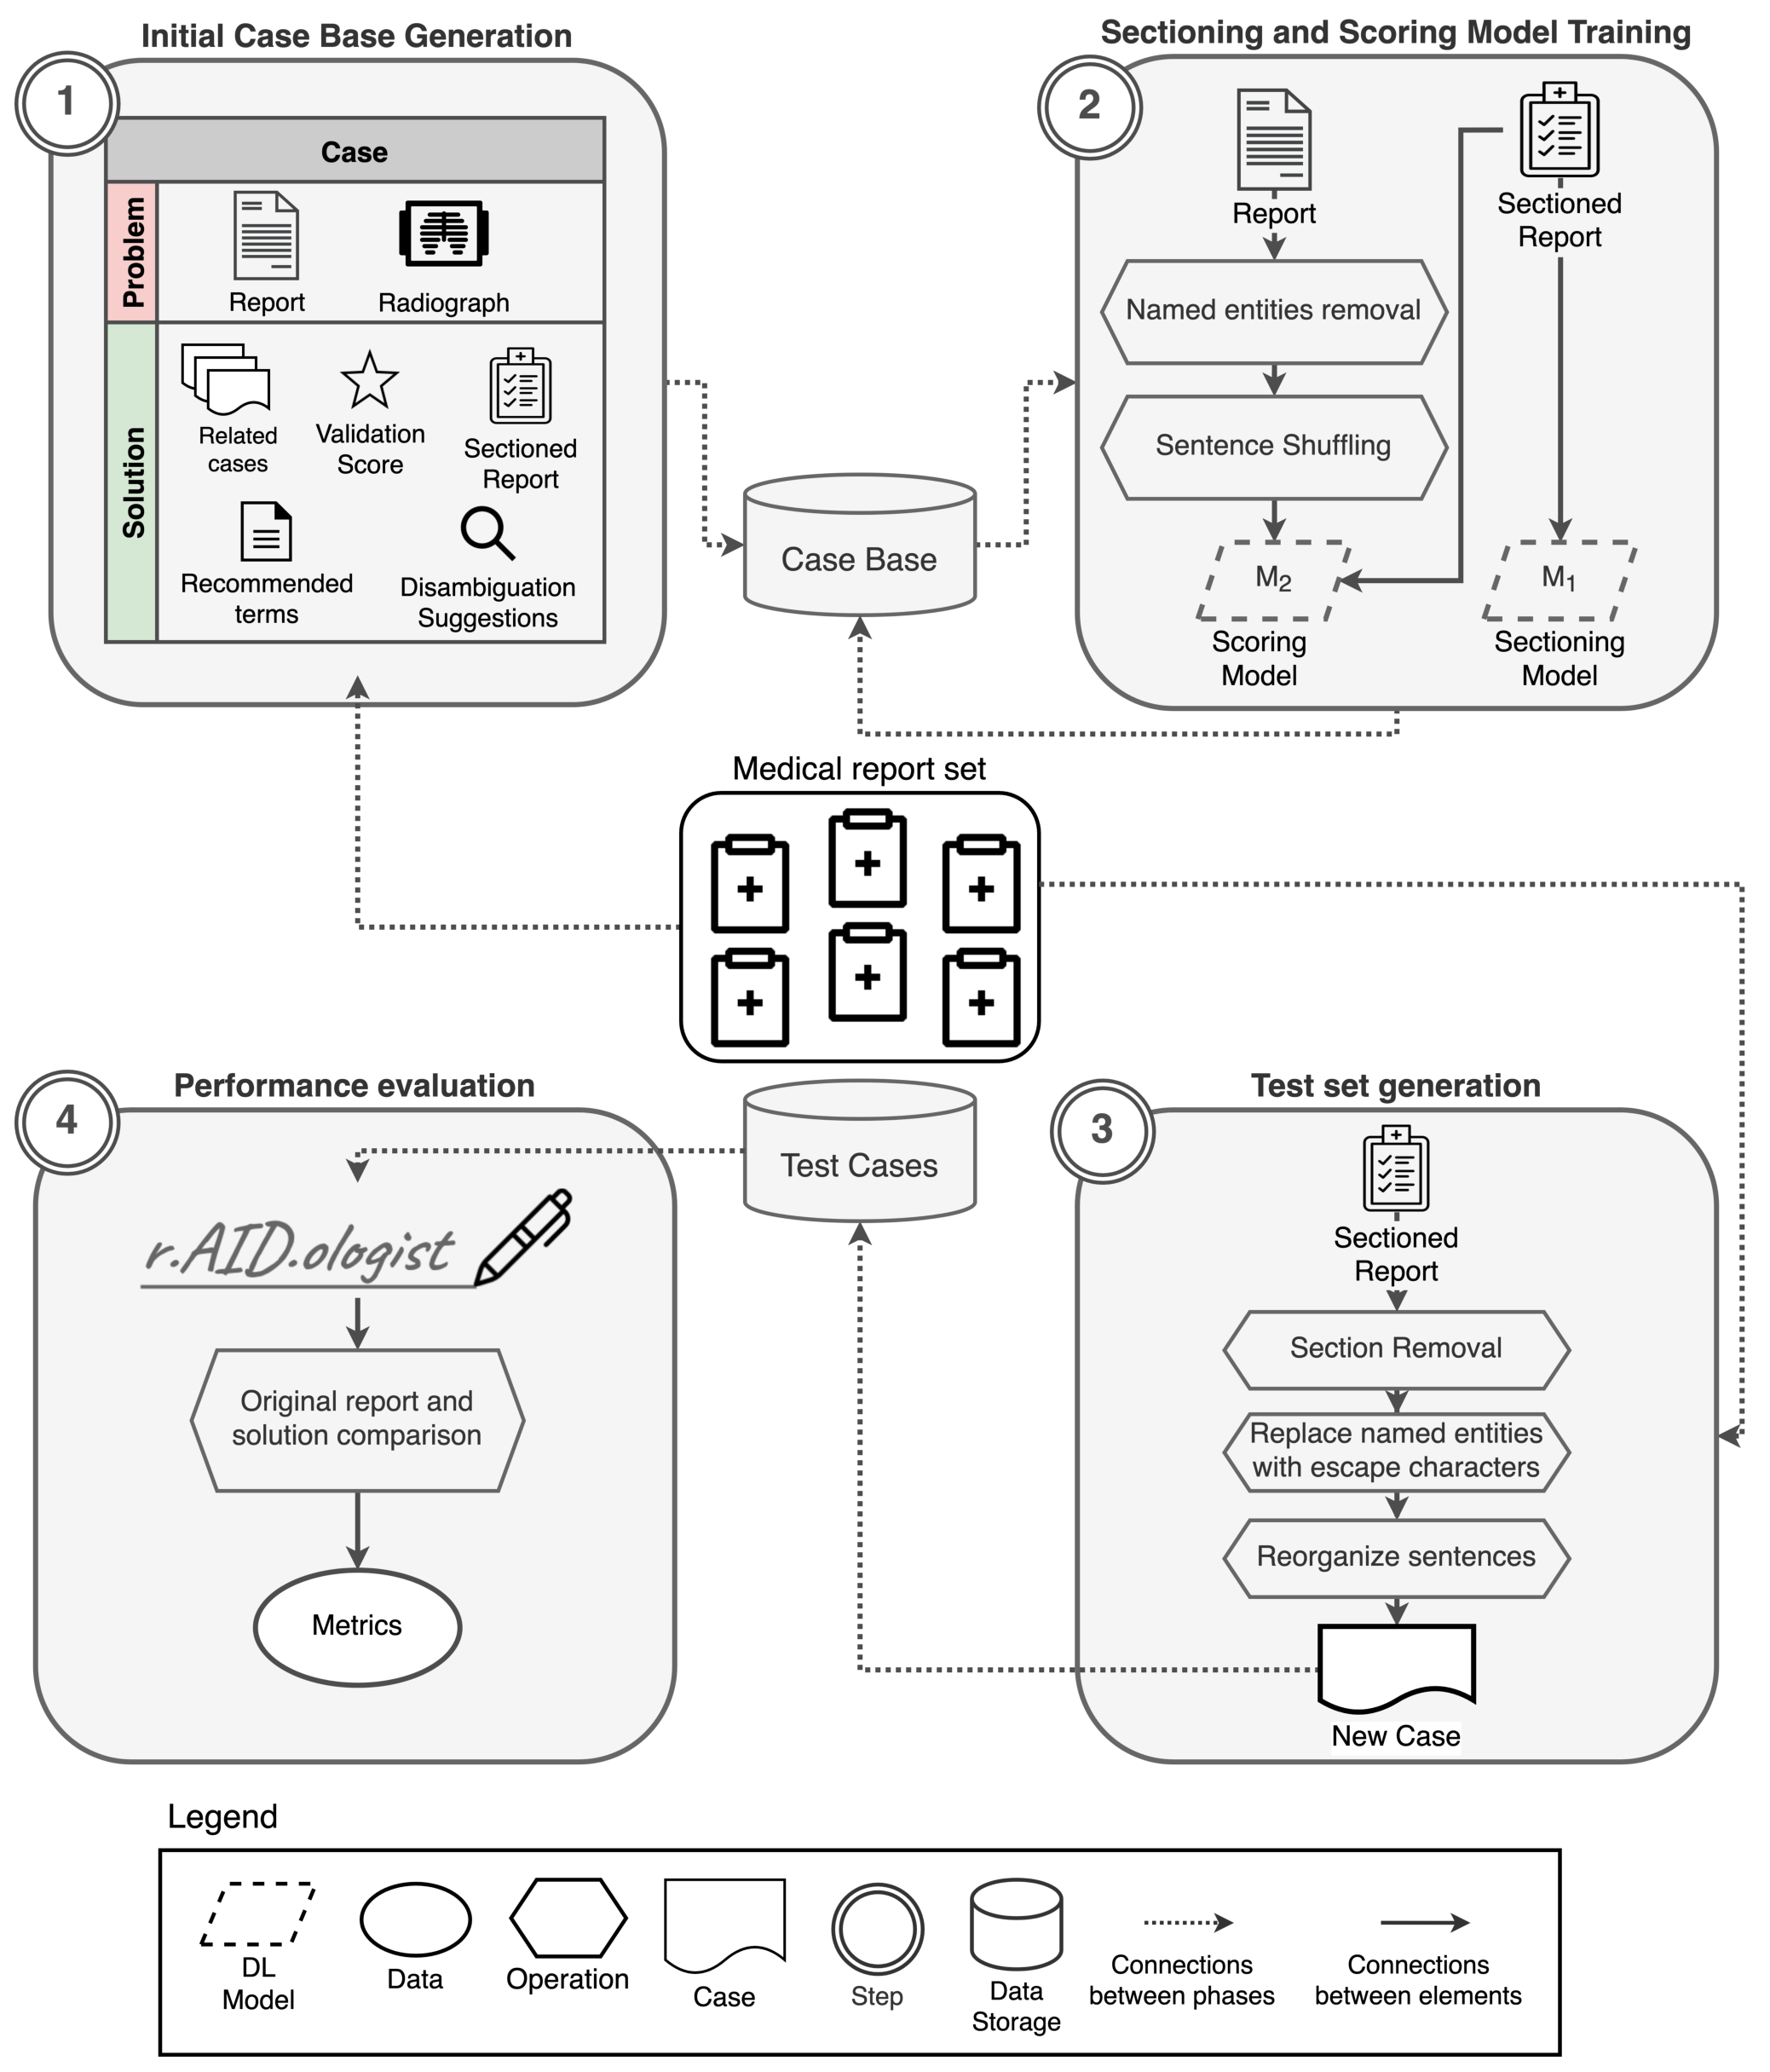
\includegraphics[width=.8\linewidth]{5_dlintegrationkbs/figures/raidologist_experimentation_overview.eps}
    \caption{Overview of the evaluation of r.AID.ologist.}
    \label{fig:overview_experimentation_raidologist}
\end{figure}

Figure \ref{fig:overview_experimentation_raidologist} depicts the four steps of the evaluation process:

\begin{enumerate}
    \item \textit{Initial case base generation.} The case base is the core of any CBR model. In the first step, a set of medical reports is converted into cases, generating the initial case base. Out of all the available medical reports, a sub-sample is selected for later testing. Reports selected for testing are not included in the case base. Each training medical report is then stripped, whenever possible, from its sections to generate the case problem. If a list of named entities or abbreviations is provided alongside the report, these are also included alongside the report in the problem case. If there are radiographs attached to the images, they are included in the case problem as well. The solution to the case is the original medical report. The remaining case solution elements are generated in the following step.
    
    \item \textit{Sectioning and scoring model training.} At this stage, cases contained in the case base are not complete, as they only contain the input problem and one element of the solution (the sectioned report). However, the original and corrupted version of the report are enough to properly train both the sectioning and scoring models. Cases contained in the case base are divided following a 80/20 proportion into two sets: training and validation. The same scoring and sectioning models described in Section \ref{5_sec:raidologist} are used in the evaluation. The sectioning model is trained using case solutions, where each report is split into sentences, and each sentence is labelled according to the section where it was featured. In the scoring model, both the problem and solution of the case are required, as this model feeds positive and negative samples. Case problems comprise the negative sample set, while case solutions are used for its positive counterpart. Section removal and sentence shuffling are also applied for further corruption. Once both sectioning and scoring models are trained, the scoring model is used to update the validation score of each case on the case base. Named entities, disambiguations and related cases are also updated as described in Section \ref{5_sec:raidologist}.
    
    \item \textit{Test set generation.} Test cases are created from the medical reports sampled for this purpose in Step 1. In the devised evaluation, the effectiveness of the model is computed based on whether, given a corrupted version of the original report, the framework is capable of providing suggestions and corrections whose application leads to a version as similar to the original report as possible. For each element in the test set, the following corruption operations are performed to create the case problems: section removal, named entity replacement by escape characters and sentence shuffling.
    
    \item \textit{Performance evaluation.} Test cases are then processed by the system, which generates a corrected version of the input report. Additionally, a list of recommended terms and potential disambiguations is provided. The corrected version of the input, corrupted report is then compared to the original version. The model should be capable of reorganizing the sentences into sections in a cohesive order, as well as suggesting the introduction of the named entities that were previously stripped from the report. The following metrics are then computed:
    \begin{enumerate}
        \item The validation score provided by the model before and after applying the corrections.
        \item The Levenshtein distance between the original report and the suggested correction.
        \item The proportion of entities detected on the original reported whose inclusion is suggested.
    \end{enumerate}
\end{enumerate}


Two different radiology datasets are considered for evaluation: MIMIC-CXR \citep{mimic-cxr} and Open-I's radiololgy set, ECGEN \citep{openi}. MIMIC-CXR contains medical reports in plain text format, without including any additional information. ECGEN provides both images and named entities alongside the medical report, as well as additional metadata. From each dataset, two initial case bases are generated, composed by 50 and 200 cases, respectively. Cases are generated from a random sampling of reports from each considered dataset. 

\begin{figure}[t!]
    \centering
    \subfigure[ECGEN 50-case set \label{fig:ecgen_validation_50}]{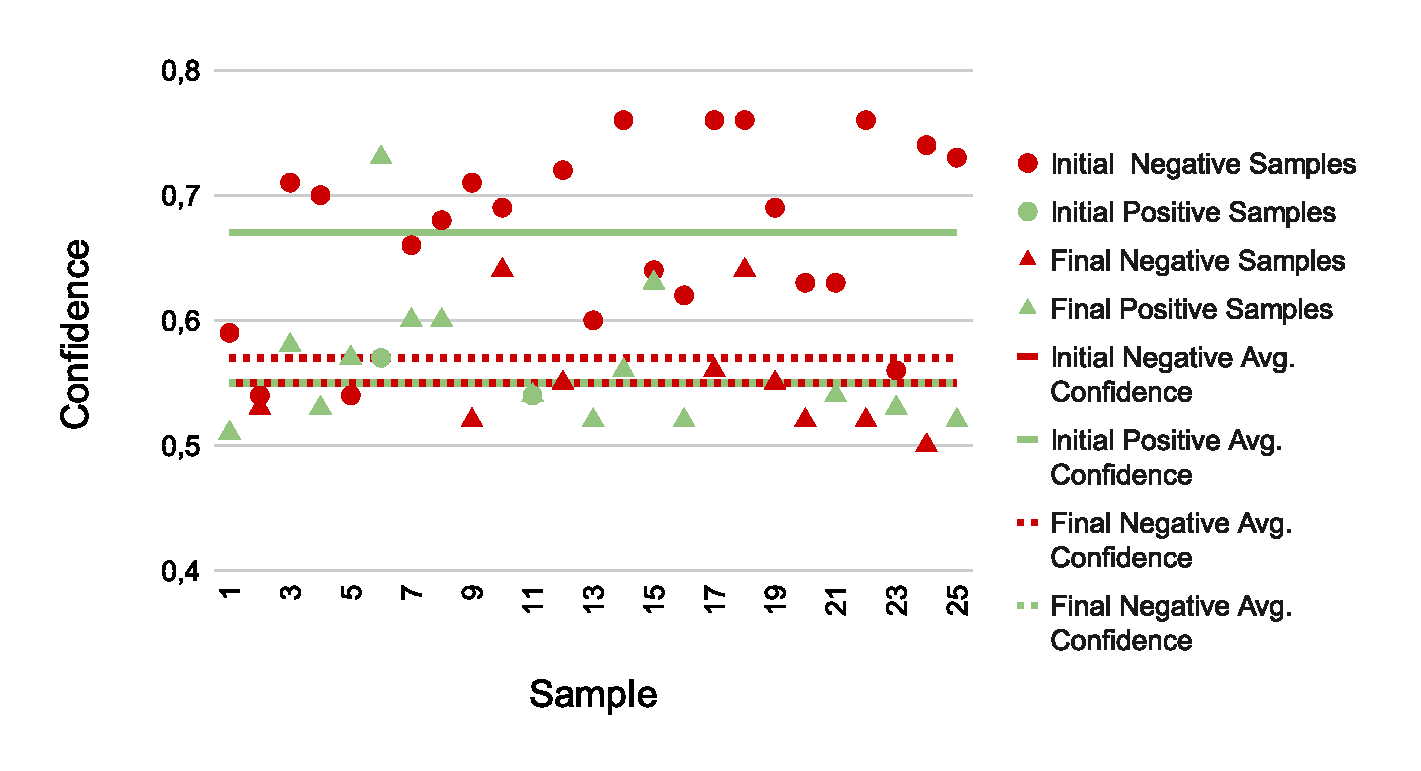
\includegraphics[width=.85\columnwidth]{5_dlintegrationkbs/figures/ecgen_50_validation.eps}}
    \subfigure[MIMIC-CXR 50-case set \label{fig:mimic_validation_50}]{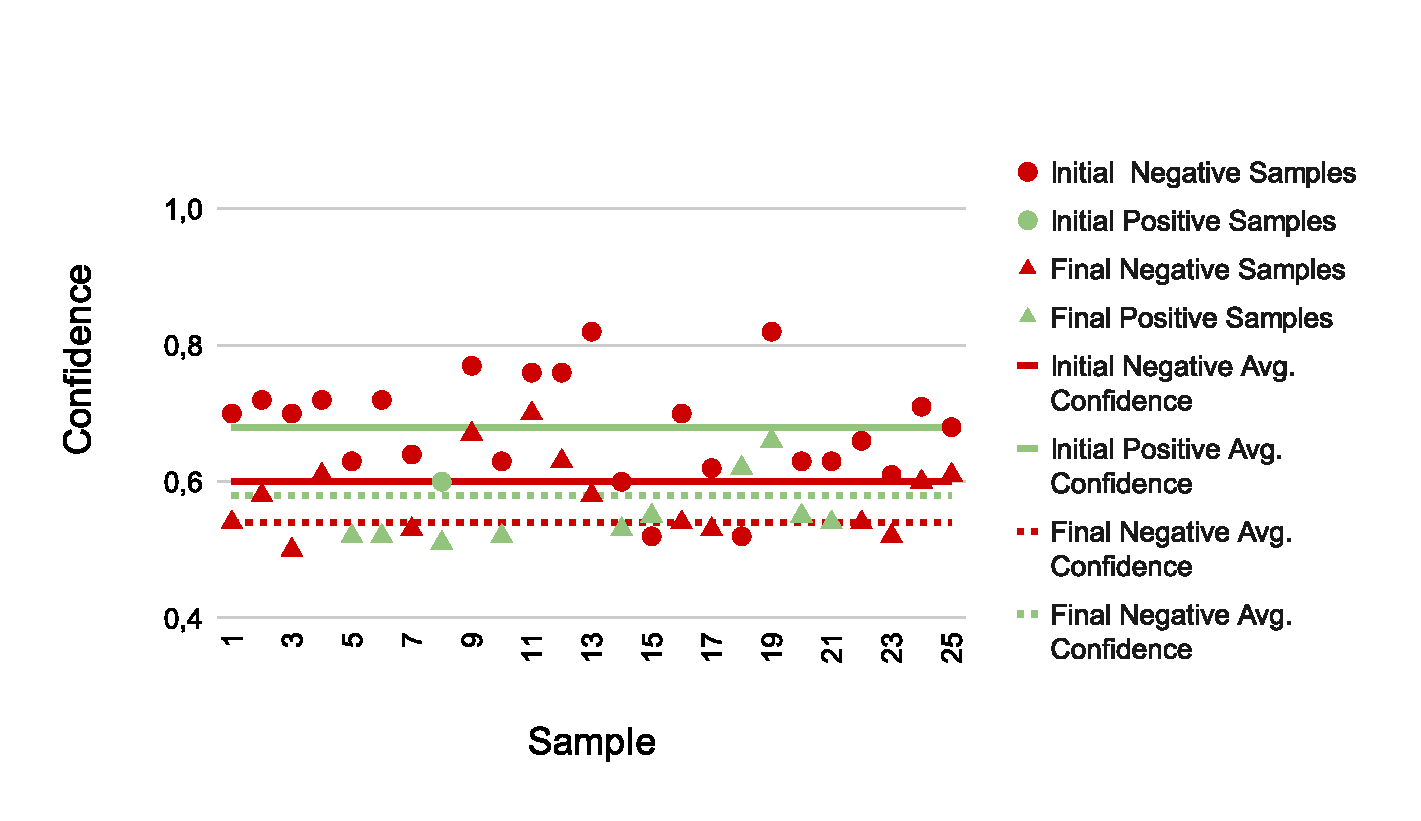
\includegraphics[width=.85\columnwidth]{5_dlintegrationkbs/figures/mimic_50_validation.eps}}
    \caption{Validation status on the 50-case set before and after corrections for the studied datasets.}
    \label{fig:50_set_comparison}
\end{figure}

The initial 50-element case base serves as a baseline to assess the performance of the framework with a limited number of cases. Applying the retain criteria in this scenario may not have any impact, as most cases may be related between them. In the 200-element case base, where the amount of initial cases is four times the size of the prior case base, retain criteria can be successfully applied, obtaining the optimal case base that contains the minimum cases to ensure maximum coverage. The optimal case bases of MIMIC-CXR and ECGEN contain 187 and 90 elements, respectively. Both the baseline and optimal case base are considered for evaluation.

\begin{figure}[t!]
    \centering
    \subfigure[ECGEN optimal case set \label{fig:ecgen_validation_optimal}]{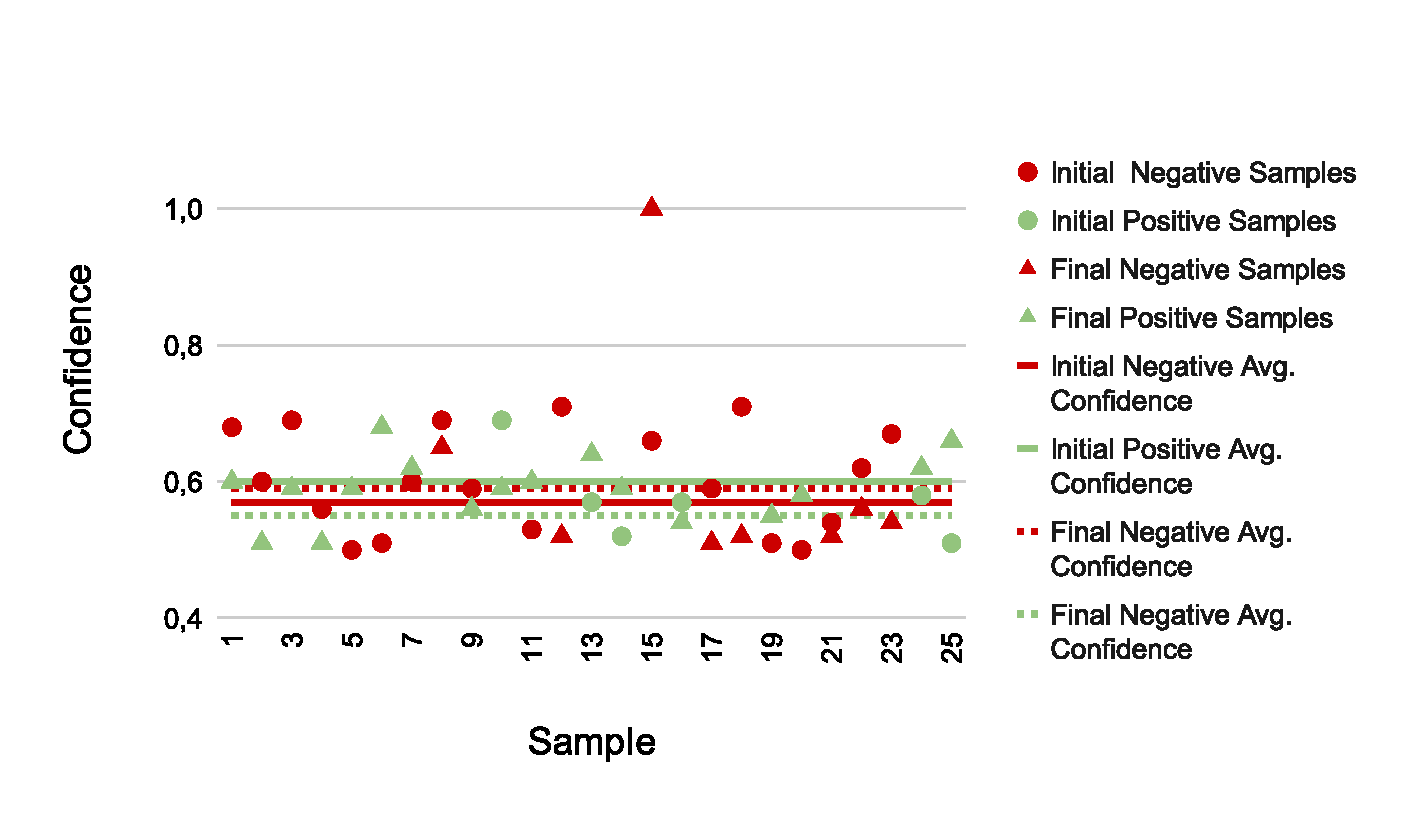
\includegraphics[width=.85\columnwidth]{5_dlintegrationkbs/figures/ecgen_optimal_validation.eps}}
    \subfigure[MIMIC-CXR optimal case set \label{fig:mimic_validation_optimal}]{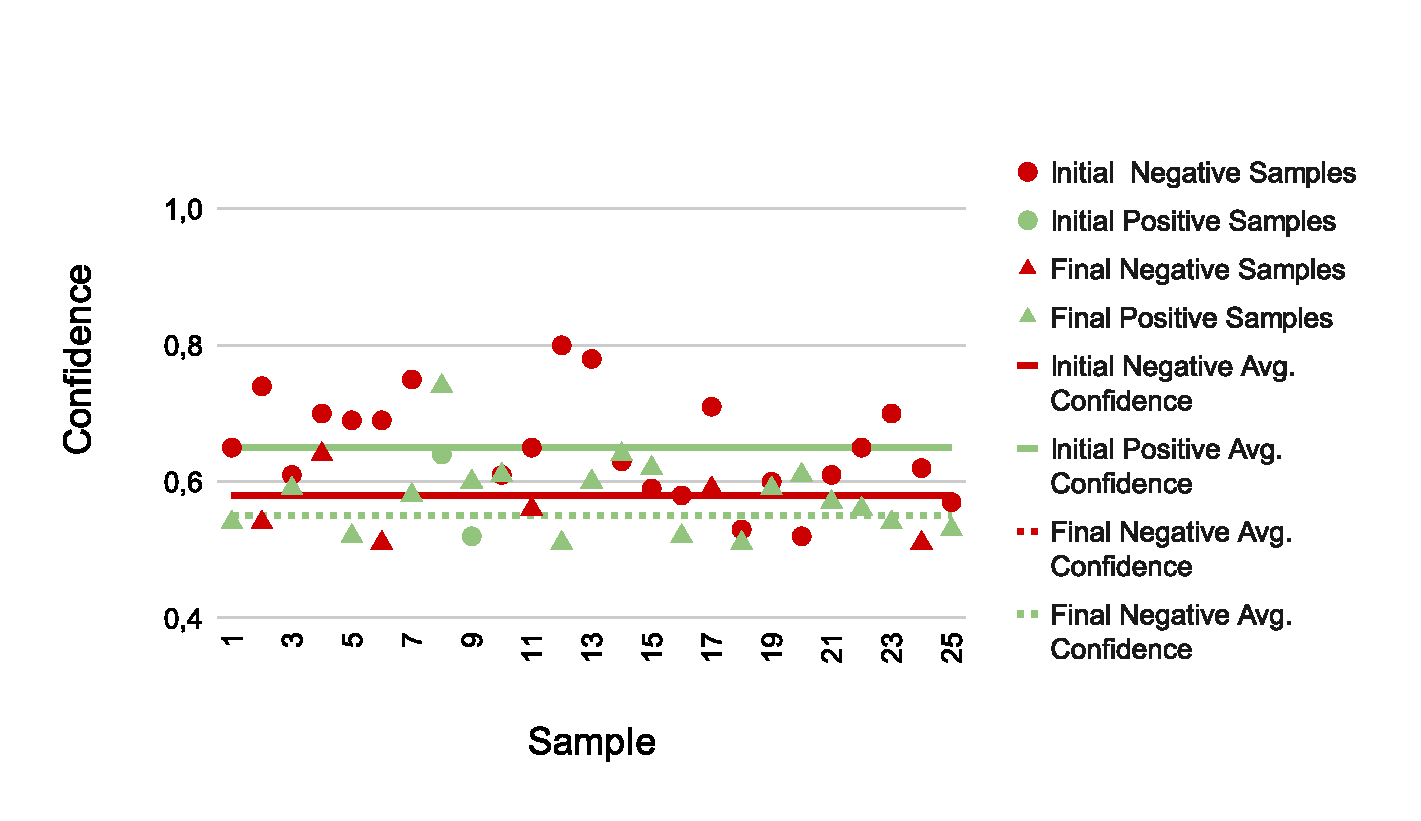
\includegraphics[width=.85\columnwidth]{5_dlintegrationkbs/figures/mimic_optimal_validation.eps}}
    \caption{Validation status on the optimal set before and after corrections for the studied datasets.}
    \label{fig:optimal_set_comparison}
\end{figure}


Figure \ref{fig:50_set_comparison} showcases the performance of the model on the 50-case base per dataset regarding report validation. Despite the limited number of cases in the case base, the framework still achieves noteworthy results, accurately correcting most of the initially invalid cases. In ECGEN (Figure \ref{fig:ecgen_validation_50}) the impact of the correction can be clearly observed, where most of the initial cases that were rated as invalid with a high confidence value turn into valid cases after applying the corrections. For MIMIC-CXR, the improvement is not as noticeable, as some cases are still rated as invalid after applying the system corrections. However, as depicted in Figure \ref{fig:mimic_validation_50}, even in those cases still denoted as invalid after applying the corrections, the confidence value diminishes dramatically. This decrement evidences that, even though the generated solution is still marked as invalid, the system corrections significantly improve the initial report.


As shown in Figure \ref{fig:optimal_set_comparison}, optimizing the case base positively impacts the performance of the model. After optimization, the results are slightly more polarized than in the previous case, as the majority of the initially invalid cases are corrected and validated when processed by the framework. Moreover, the overall confidence values increase with respect to that of the 50-case set, indicating that the scoring model learns to better differentiate valid and invalid cases. Additionally, optimizing the case base also soothes the existing differences in performance. While in the 50-case set the results obtained in ECGEN are slightly better than the ones achieved in MIMIC-CXR, when optimizing both case bases their performances in terms of report validation become fairly similar.

\begin{figure}[t!]
    \centering
    \subfigure[ECGEN \label{fig:ecgen_levenshtein}]{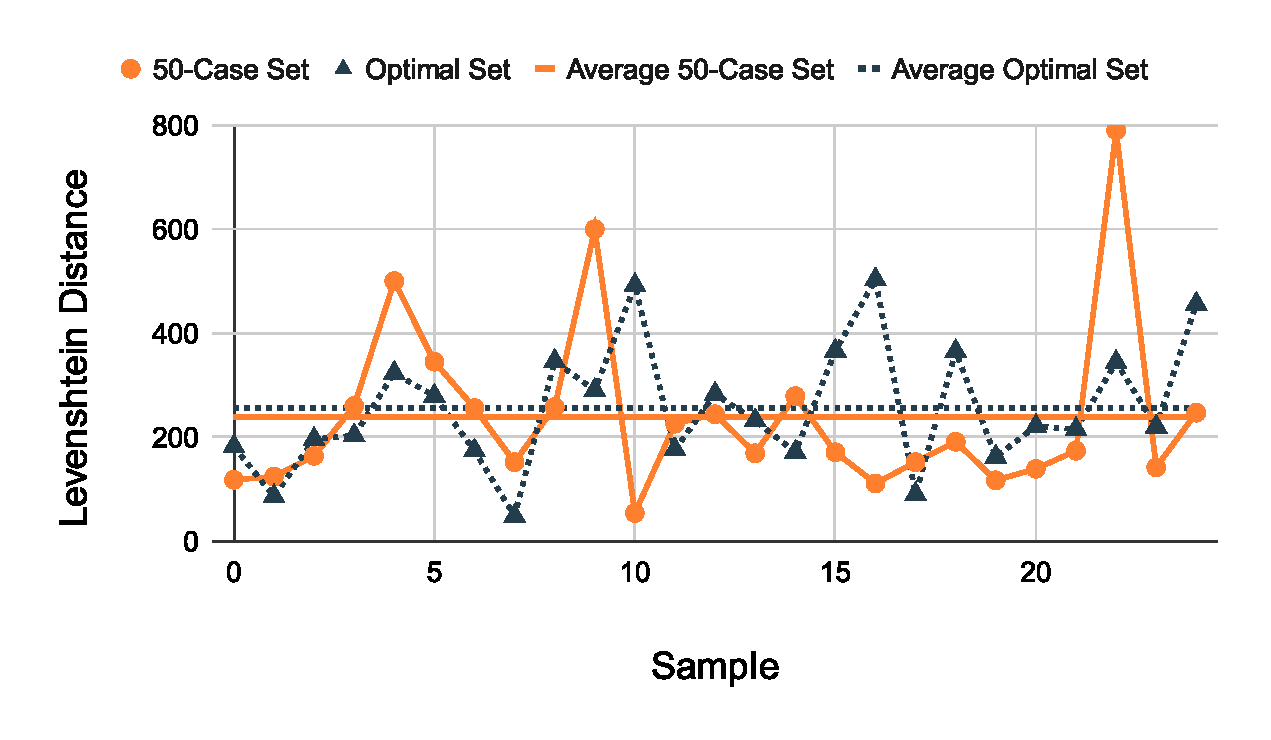
\includegraphics[width=.75\columnwidth]{5_dlintegrationkbs/figures/ecgen_levenshtein.eps}}
    \subfigure[MIMIC-CXR  \label{fig:mimic_levenshtein}]{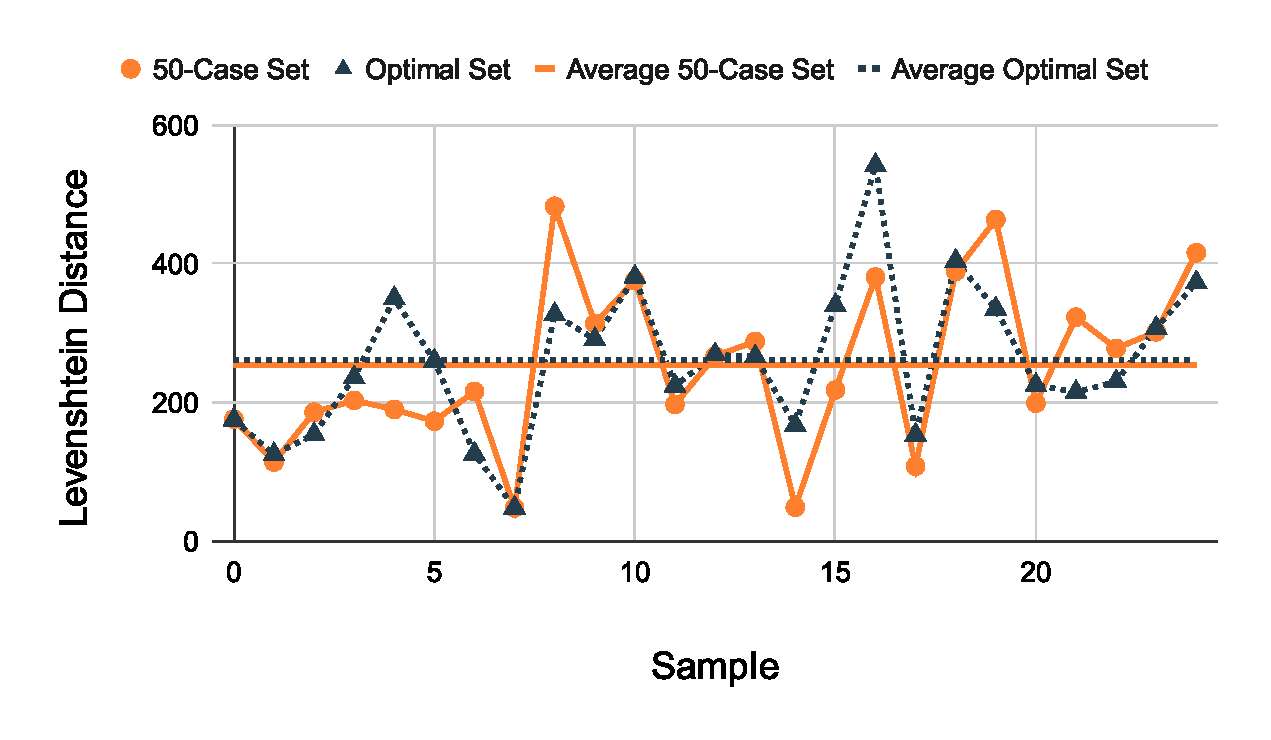
\includegraphics[width=.75\columnwidth]{5_dlintegrationkbs/figures/mimic_levenshtein.eps}}
    \caption{Levenshtein distance per sample on each studied dataset.}
    \label{fig:levenshtein_comparison}
\end{figure}


Levenshtein distance \citep{levenshtein} between each original and corrected report pair is also computed. Different text similarity metrics could be considered for evaluation, such as cosine similarity or Jaccard index. However, none of these metrics consider sentence ordering. As described in Figure \ref{fig:overview_experimentation_raidologist}, test cases are generated by stripping sections, permutating sentence order, and removing named entities. Therefore, even after the corruption process, both the original and corrupted versions of the report are almost equal in terms of content. An order-sensitive metric is required to ascertain the similarity degree between the original and the corrected report. Figure \ref{fig:levenshtein_comparison} reports the Levenshtein distance for each original and corrected report pair on each dataset and case base. Levenshtein distances in ECGEN (Figure \ref{fig:ecgen_levenshtein}) remain reasonably similar in both the 50-case and optimal bases between cases. Similarly, in MIMIC-CXR (Figure \ref{fig:mimic_levenshtein}) the distance between original and corrected reports remains akin. Case based optimization does not induce an additional improvement, as in the validation evaluation. This issue may be alleviated by the introduction of user input. For the evaluation, both the problem and the solution of the cases have been artificially generated. User-corrected reports may be more expressive and richer in content, enabling the identification of more complex correction patterns.

\begin{figure}[t!]
    \centering
    \subfigure[ECGEN \label{fig:ecgen_entities}]{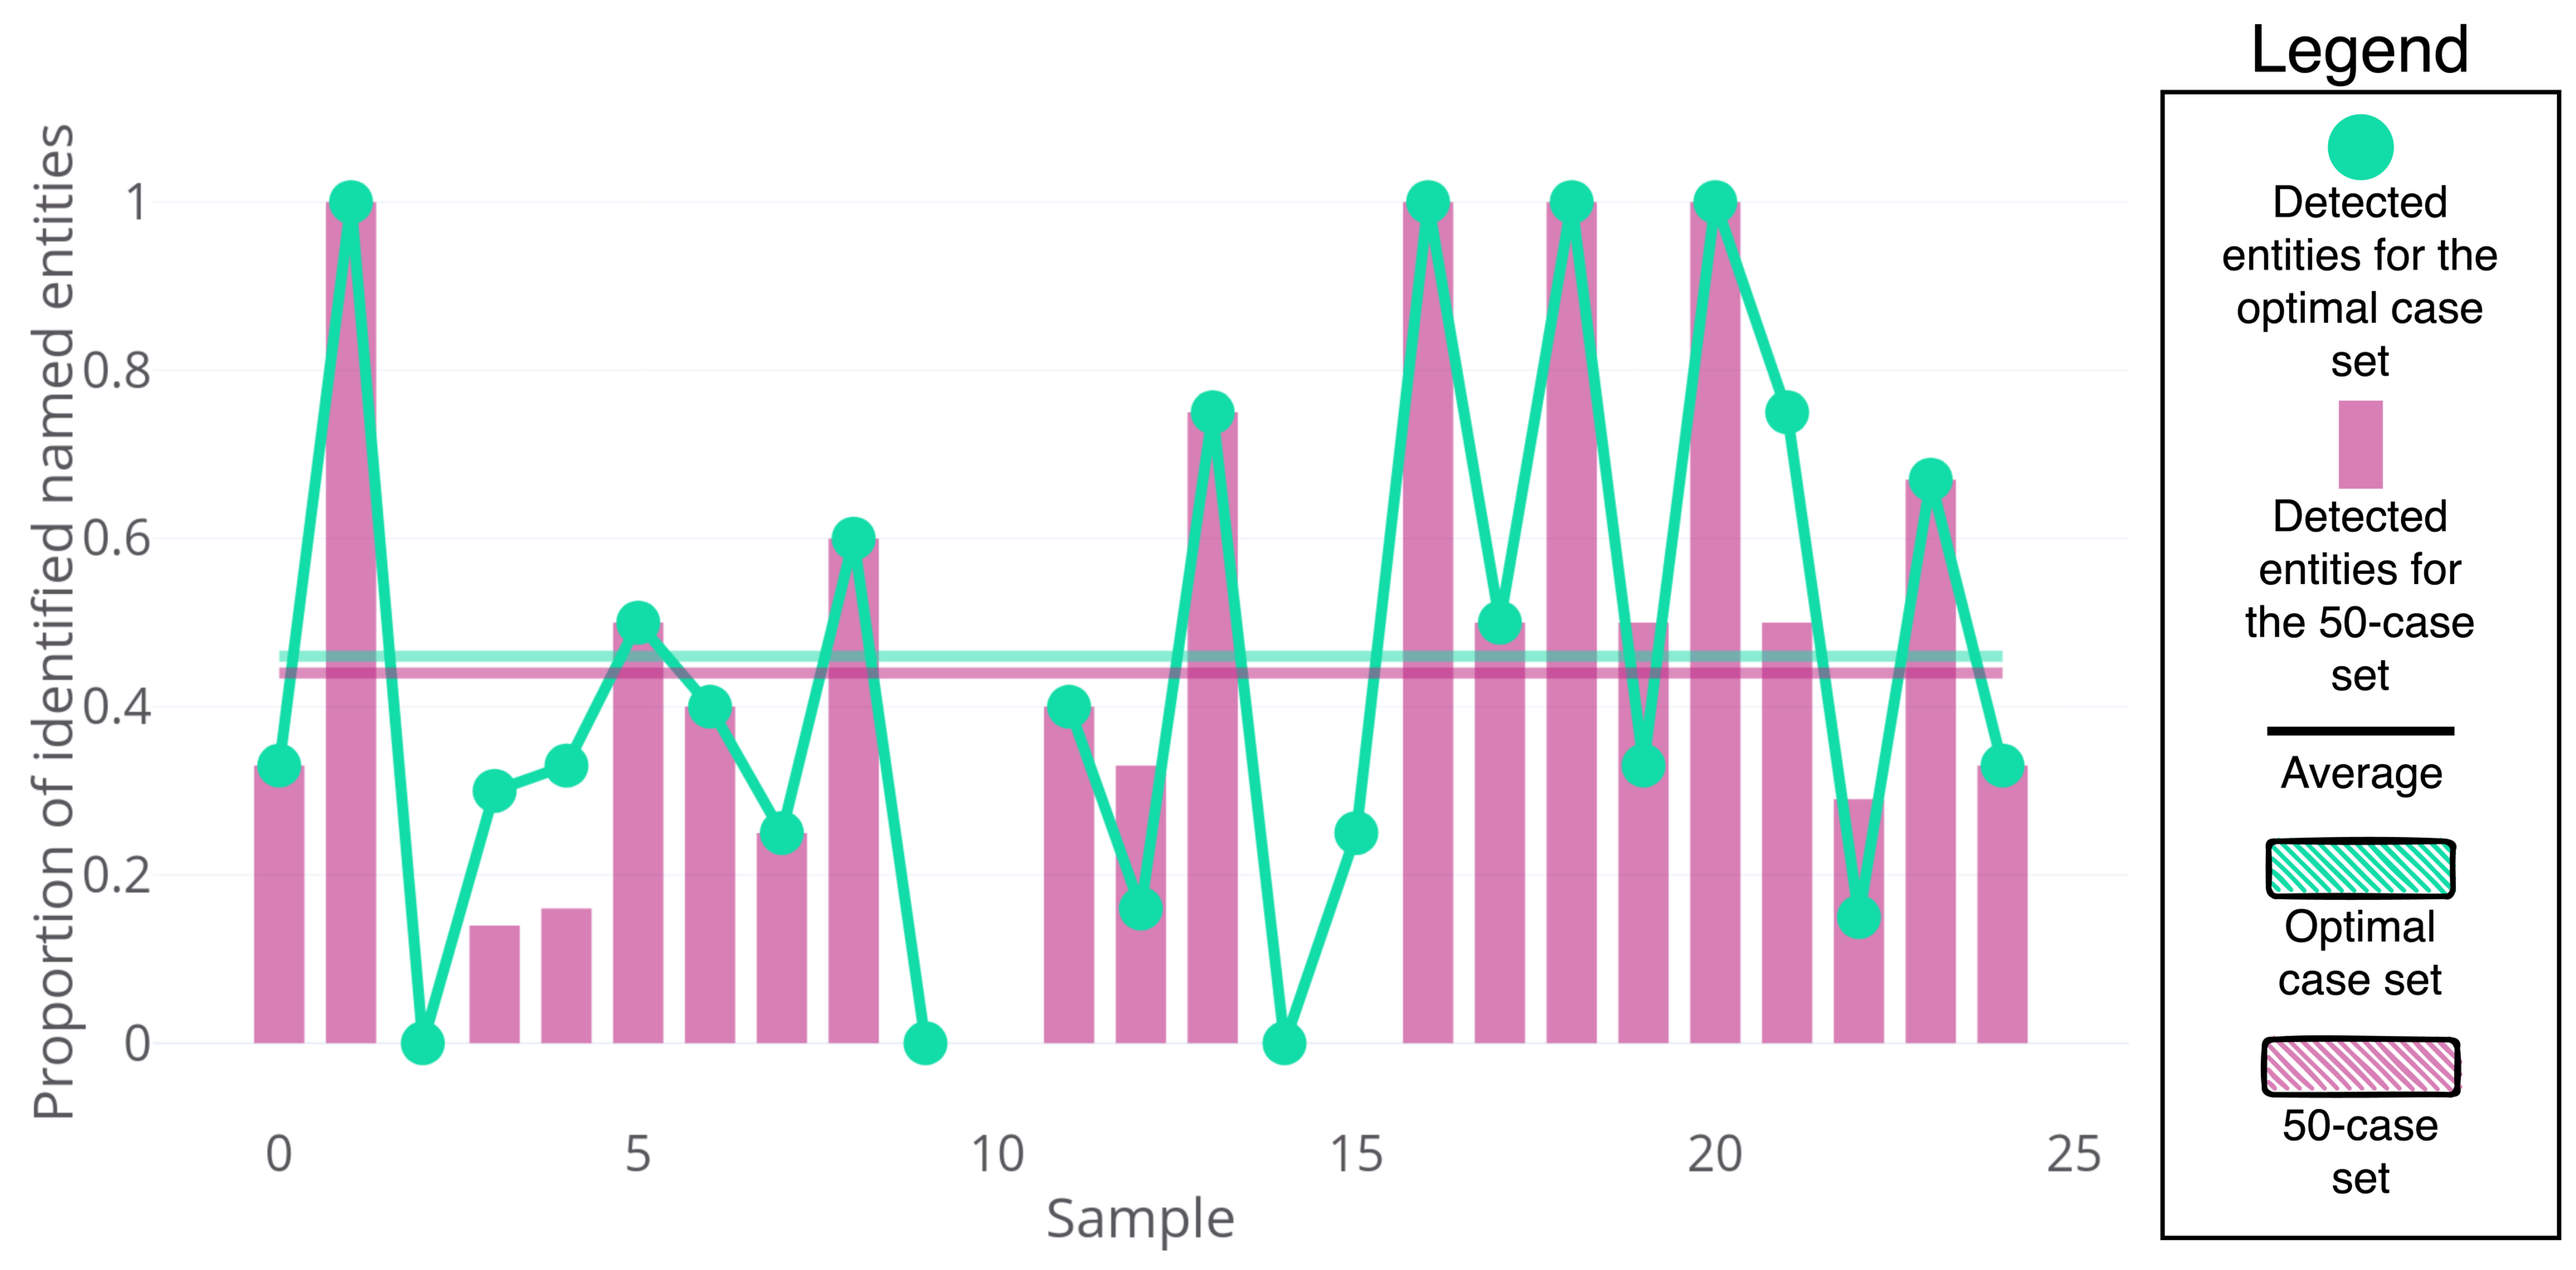
\includegraphics[width=.75\columnwidth]{5_dlintegrationkbs/figures/ecgen_entities.eps}}
    \subfigure[MIMIC-CXR  \label{fig:mimic_entities}]{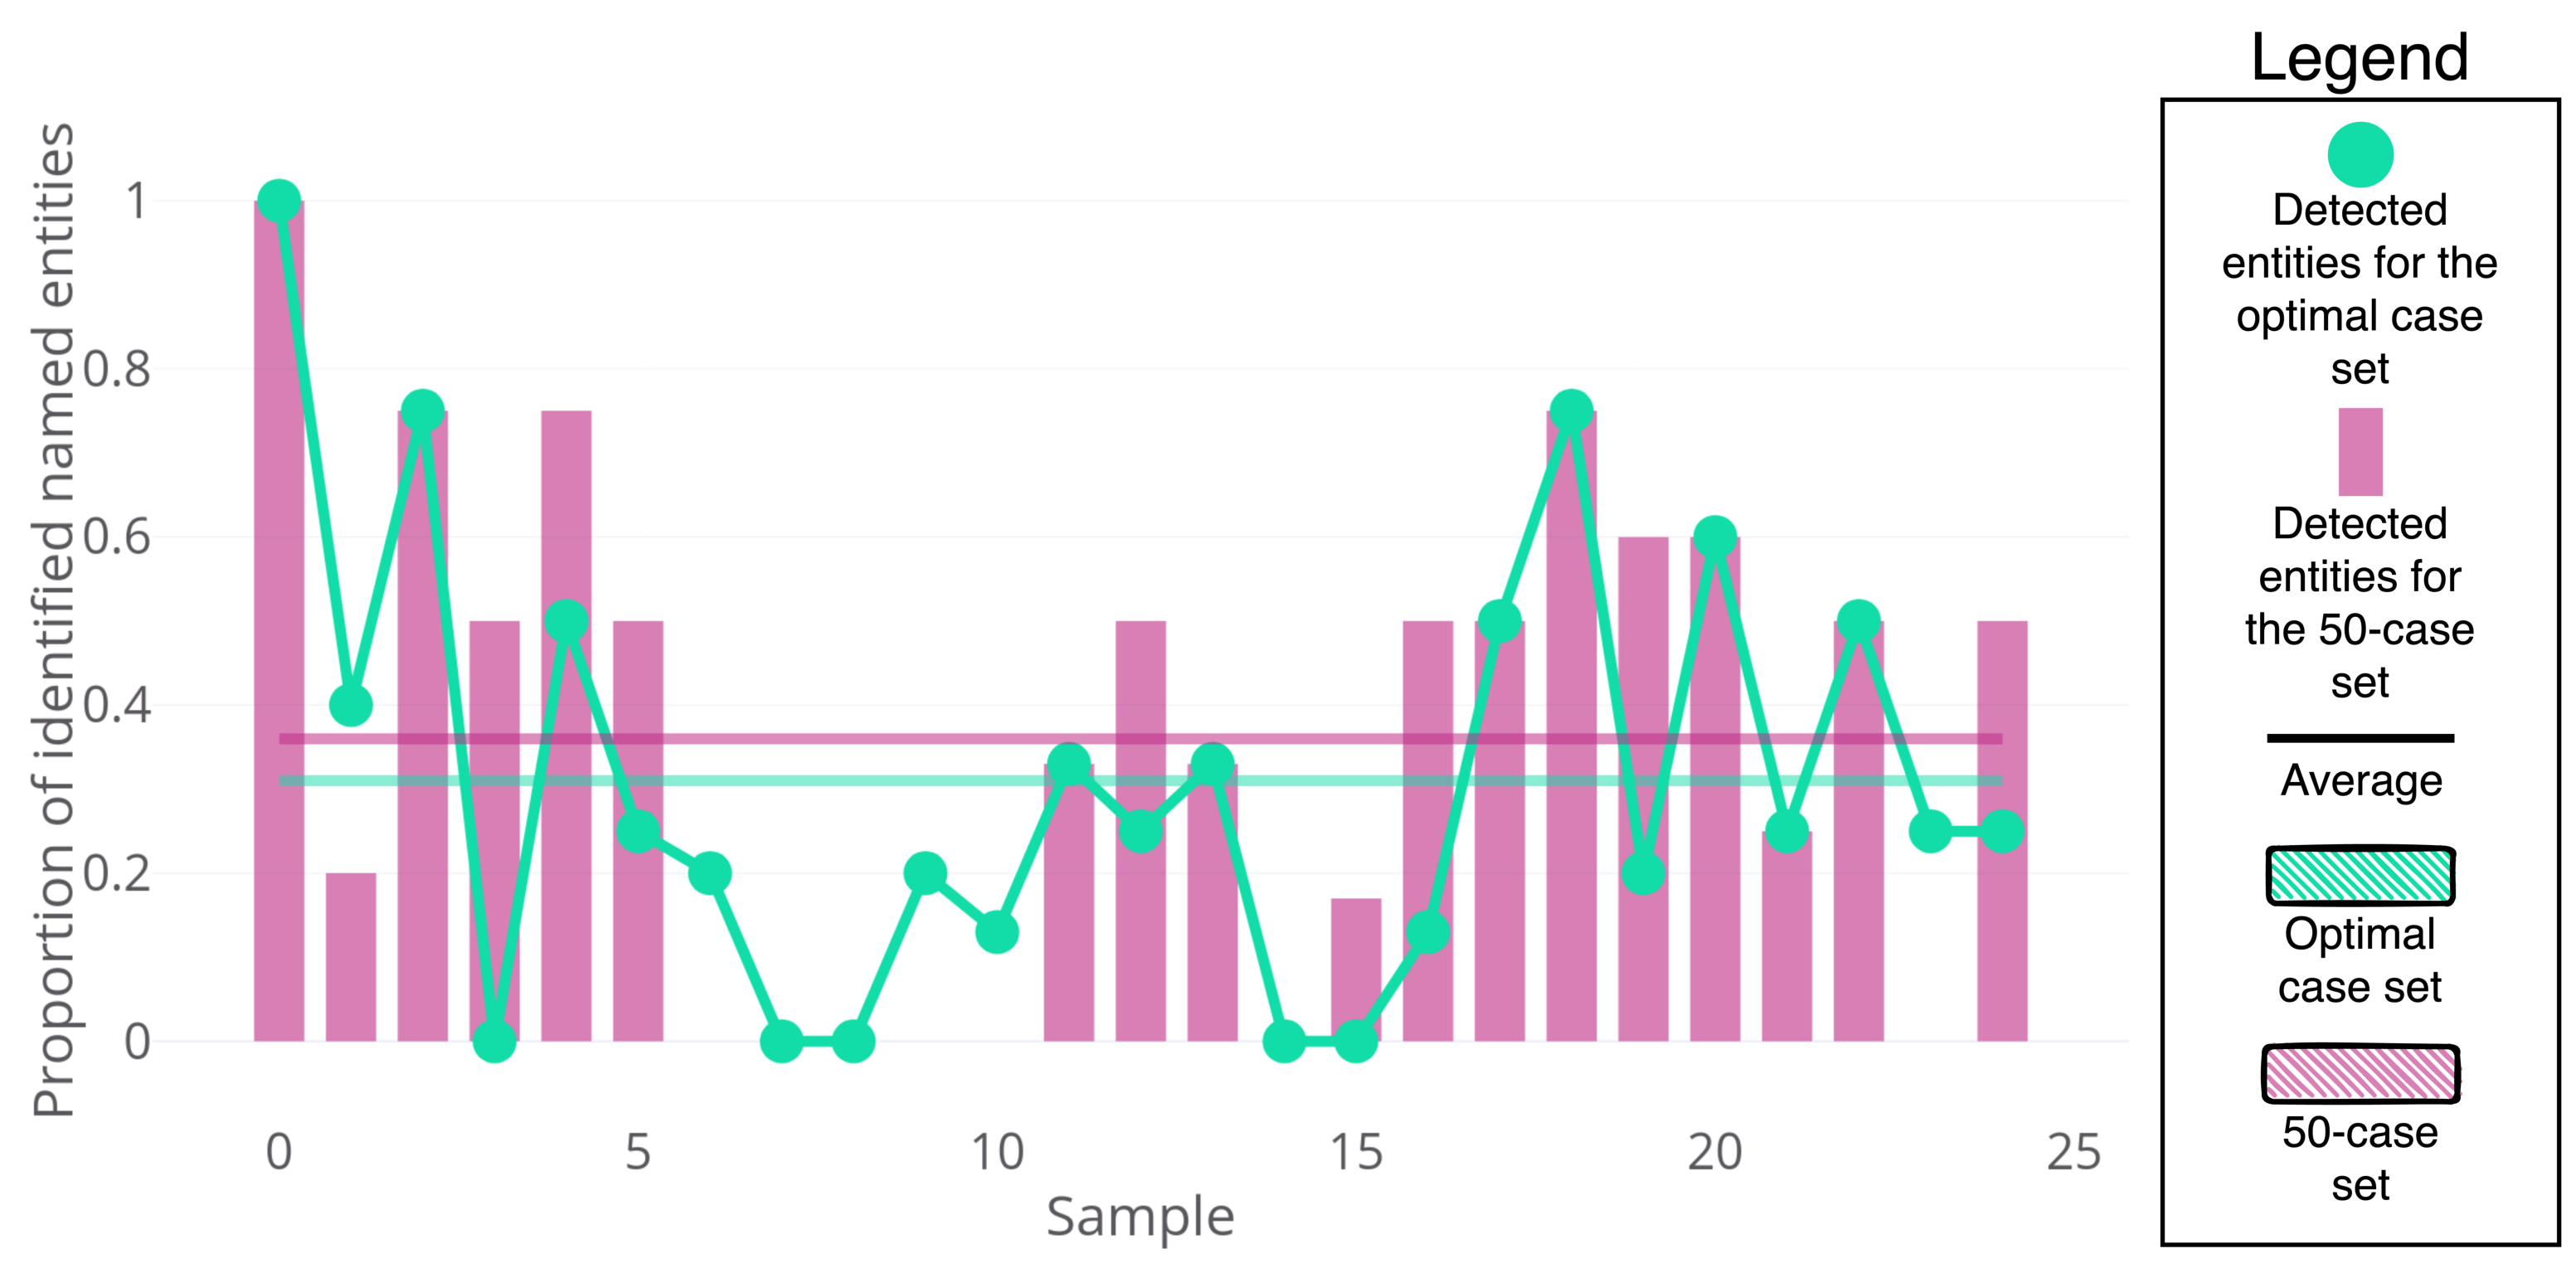
\includegraphics[width=.75\columnwidth]{5_dlintegrationkbs/figures/mimic_entities.eps}}
    \caption{Proportion of named entities correctly suggested per case on each studied dataset.}
    \label{fig:entities_comparison}
\end{figure}

Figure \ref{fig:entities_comparison} depicts the number of named entities correctly suggested by the framework. In Step 3 of the evaluation, named entities detected in the original report were replaced by escape characters as part of the corruption process. Figures \ref{fig:ecgen_entities} and \ref{fig:mimic_entities} depict the proportion of named entities stripped from the original report and correctly suggested by the system in ECGEN and MIMIC-CXR, respectively. As evidenced by the results, case base optimization induces an improvement in the number of correctly suggested entities. This phenomenon is clearly observed in ECGEN's results (Figure \ref{fig:ecgen_entities}). Only in three cases, the number of detected entities slightly decreases after case base optimization, but significantly improves in four other cases. In MIMIC-CXR (Figure \ref{fig:mimic_entities}), the result is not as consistent as in the previous dataset, which could be due to the difference in the size of the optimized case base between the two datasets. MIMIC-CXR has double the number of cases in its optimized version that ECGEN. Named entities are suggested based on the top $k$ similar cases. Hence, if the retrieved similar cases contain few named entities, it directly impacts the number of suggestions provided by the system. Increasing the value of $k$ in the retrieval could potentially correct this issue.

\color{black}
\subsection{Design Compliance}\label{5_sec:design_compliance}
A Case-based reasoning model comprising several boosting DL modules instantiates the insertion proposal in Section \ref{5_sec:dl_intro_kbs_methodology}. Figure \ref{fig:compliance_dl_into_kbs} denotes the specific method design parameters of the proposed framework, which are described as follows:

\begin{figure}[t]
    \centering
    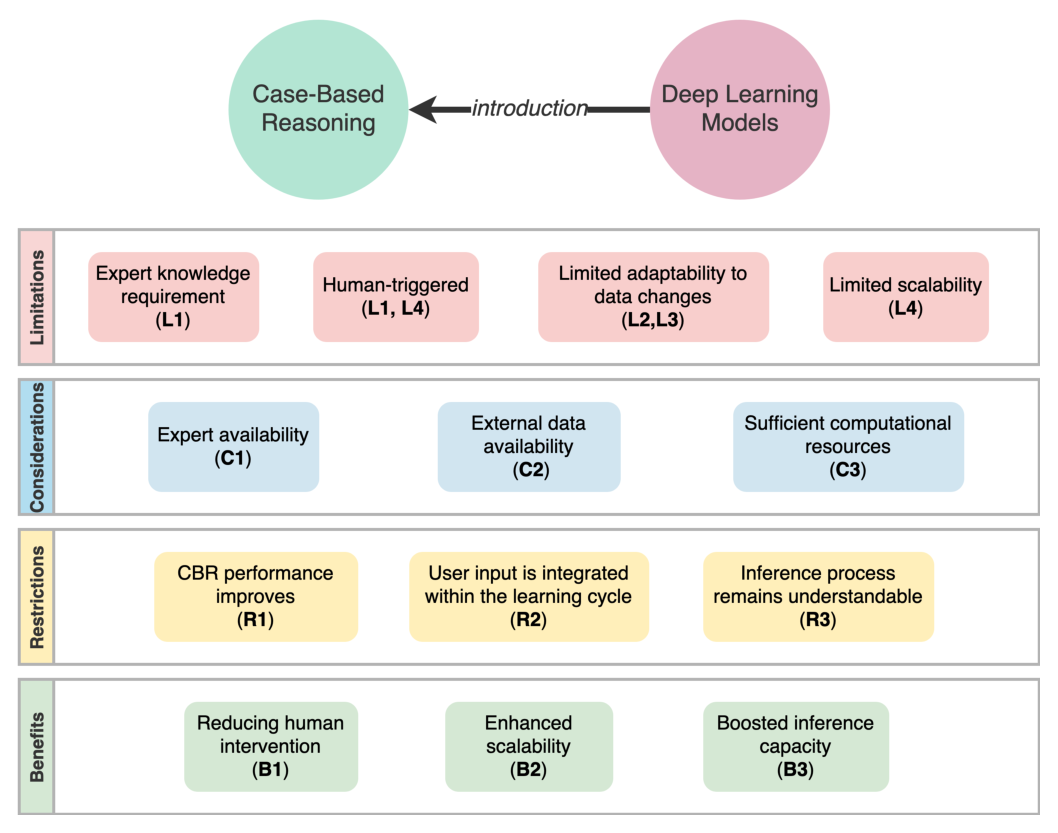
\includegraphics[width=\linewidth]{5_dlintegrationkbs/figures/Instance_DL_intro_KBS.eps}
    \caption{Overview of the design parameters of the introduction of DL models into a CBR framework. In bold, the general design parameters as depicted in \ref{fig:overview_dl_kbs_intro}.}
    \label{fig:compliance_dl_into_kbs}
\end{figure}

\paragraph{Limitations}
\begin{itemize}
    \item \textbf{Expert knowledge requirement.} CBR models are highly reliant on expert input. This is particularly remarkable in the revise stage, where a panel of experts needs to manually revise the pending cases to make their inclusion in the case base effective (\ref{dl_intro_kbs_L_human}). In CBR, the system improves with the inclusion of new cases within the system. Subsequently, if no expert knowledge is available to validate the cases, the model performance remains static. 
    
    \item \textbf{Human-triggered.} In a pure CBR model, several stages are only triggered by human intervention (\ref{dl_intro_kbs_L_human}). Except in the retrieval phase, where the user can be actively involved, its influence can extend to different phases, such as revise and retain. Subsequently, the learning process may be hampered if no human intervention is available (\ref{dl_into_kbs_L_scalability}).
    
    \item \textbf{Limited adaptability to data changes.} Rule-based systems are used on a general basis in CBR models. Usually, during the reuse phase, a set of rules inferred from the existing cases is applied to devise a valid solution for the input problem. Hence, rules are only effective when the input problem resembles an existing case (\ref{dl_into_kbs_L_brittle}). The usage of rules limits the abstraction level achieved by the model to devise tailored solutions to the input problems (\ref{dl_into_kbs_L_abstraction}).
    
    \item \textbf{Limited scalability.} Reliance on expert knowledge can create a bottleneck in the system, as cases need to be manually revised before their inclusion in the case base (\ref{dl_into_kbs_L_scalability}). Similarly, in the reuse phase, the use of rule-based systems considerably limits the scalability of the system, as the rules need to be constantly updated to cover upcoming changes in the cases.
    
    
\end{itemize}
\paragraph{Considerations}
\begin{itemize}
    \item \textbf{Expert availability.} In the health domain where the proposed implementation is deployed, expert knowledge is crucial for the correct behaviour of the system. Users are not required to be experts to use the system, and therefore expert knowledge must be integrated within the system so that the output is still valid. Expert knowledge must be available, at least in the initial timeline of the system, to ensure the validity of the output responses and the correct behaviour of the system (\ref{dlintrokbs_C_expert}).
    
    \item \textbf{External data availability.} DL models are data hungry, thus requiring large datasets to achieve a good performance. In the initial stages of the CBR, where the case base is not reasonably populated, the amount of available data may not be sufficient to train robust DL models. Therefore, external data may be required to train the DL model until the number of cases available is enough to replace it (\ref{dlintrokbs_C_data}).
    
    \item \textbf{Sufficient computational resources.} CBR models do not entail elevated computational power, but require sufficient storage. On the contrary, DL models may demand a higher computational power to be able to operate. Therefore, it must be ascertained that both the storage and computational resources are sufficient (\ref{dlintrokbs_C_resource}).
    
\end{itemize}
\paragraph{Restrictions}
\begin{itemize}
    \item \textbf{Case-based reasoning model performance improves.} The introduction of DL models carries a computational cost. This increment in cost must be reflected in a noticeable improvement in the performance of the model to maintain a balance between benefit and cost. The proposed framework satisfices this constraint, as the inclusion of DL models induces the generation of case solutions that cannot be inferred otherwise (\ref{dlinstrokbs_R_performance}).
    
    \item \textbf{User input is integrated within the learning cycle.} CBR models are user-oriented, and therefore the validity of a given solution is not objective, but subjective to the user requirements and expectations. Subsequently, user input must play an important role in the generation of the case solution, and should be considered by the different modules to adjust their outputs accordingly. In the proposed framework, user input not only guides the retrieval process, but it is also required to correct and validate the initially proposed solution (\ref{dlintrokbs_R_user}). 
    
    \item \textbf{Inference process remains understandable.} One of the key advantages of symbolic models with respect to their subsymbolic counterparts are their transparency and interpretability. This property should be therefore preserved. In the proposed implementation, DL models are included seamlessly in the CBR cycle. Therefore, while some minor elements of the retrieve and reuse phases may be opaque, the output of each phase as a whole can be fully understood from the input (\ref{dlintrokbs_LR_interpretability}).
\end{itemize}
\paragraph{Benefits}
\begin{itemize}
    \item \textbf{Reducing human intervention.} Expert knowledge is essential in the early learning stages of the CBR model to compensate the lack of cases contained in the case base. However, when the number of elements in the case base is sufficient to train robust DL models, expert knowledge may be not required as frequently. The replacement of rule-based systems by DL models reduces the need for human intervention, as DL models can automatically fit new data without external specifications (\ref{dlintrokbs_B_automatization}).
    
    \item \textbf{Enhanced scalability.} Replacing rule-based systems with DL models not only reduces the need for human intervention, but improves the scalability of the system. While rules require human intervention for validation and maintenance, thus creating potential bottlenecks, DL models operate autonomously. Therefore, reuse modules are easily and automatically kept updated with the data contained in the case base (\ref{dlintrokbs_B_scalability}).
    
    \item \textbf{Boosted inference capacity.} CBR should produce a tailored solution for a given input, which is generally obtained via rule instantiation. The solutions inferred by the rules are highly limited, as they rely on generalizations about the data, thus not capturing the particularities of each case. Moreover, they may be insufficient to deal with complex inputs where the attributes are not strictly quantitative. The inclusion of DL models not only enables the generation of solutions that could not be inferred from rules, but also enables the comparison of complex inputs, such as textual reports (\ref{dlintrokbs_B_inference}).
\end{itemize}

\section{Summary}\label{5_sec:summary}
\elvitodo{TBD cuando esté hecha la metodología para relacionar todo}

%\chapter{Knowledge Extraction from Deep Learning Models}
\label{chap:kbsextractiondl}
%ENLAZAR ESTO CON LOS PRINCIPIOS DE EXPLICABILIDAD DE PHILLIPS ET AL..
This chapter\footnote{This chapter is based on the work: References
Amador-Domínguez, E., Serrano, E., and Manrique, D. (2021). A hierarchical multi-agent architecture based on virtual identities to explain black-box personalization policies. Expert Systems with Applications, 186, 115731. doi:10.1016/j.eswa.2021.115731} showcases the extraction of knowledge from DL Models. Section \ref{6_sec:kbs_extra_dl_method} provides an overview on the design parameters of KBS extraction from DL models. Two instances of the proposed design are introduced in this chapter. The first instance focuses on \textit{black-box hyperpersonalization models} (BBHOS), DL models devised for user content personalization. Section \ref{6_sec:mas_bbhos_general} introduces this scenario, where a multi-agent system extracts behavioral patterns from the BBHOS. The MAS system is presented in Section \ref{6_sec:subsec:mas_description}, providing an example of its use in Section \ref{6_sec:subsec:case_study}. Section \ref{6_sec:subsec:mas_design_compliance} assesses the compliance of the proposed instance of the model with respect to the general method. 

Section \ref{6_sec:geni_main} outlines the second of the extraction instances. In this scenario, an explainability framework for extracting insights on the inference process of KGE models is presented. The proposed framework, GEnI, is described in Section \ref{6_sec:subsec:geni}. Sections \ref{6_sec:subsec:geni_evaluation} and \ref{6_sec:subsec:geni_results} depict the evaluation and analysis of the framework results, respectively. The compliance of the instance with respect to the general design parameters is portrayed in Section \ref{6_sec:subsec:geni_design_compliance}. Section \ref{6_sec:summary} summarizes the content of the chapter.


\section{Knowledge Extraction from Deep Learning Models}\label{6_sec:kbs_extra_dl_method}
In this context, the DL model acts as a passive element, from which the KBS is extracted by means of a middleware model. In this scenario, the extracted KBS are mostly limited to associative rules and correlations. Method design parameters for KBS extraction from DL models are depicted in Figure \ref{fig:kbs_extra_dl_overview}.
\begin{figure}[t]
    \centering
    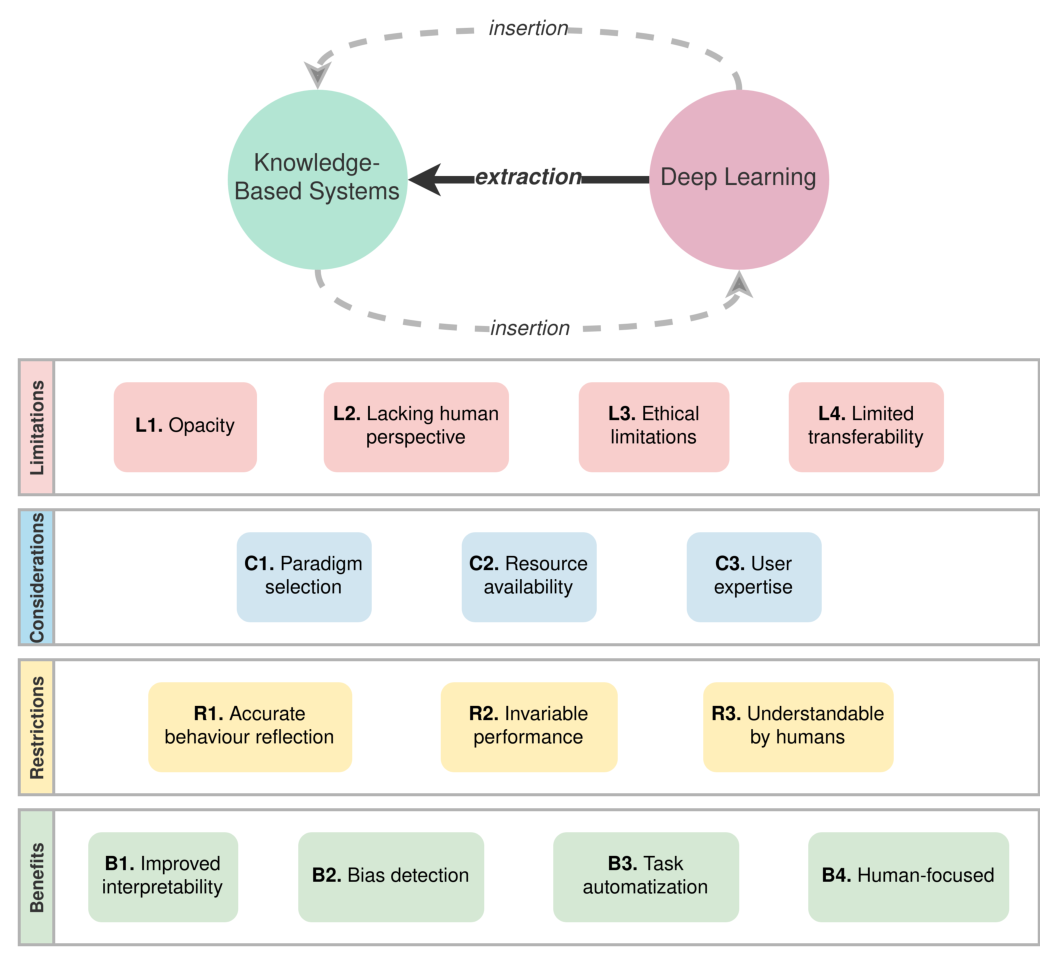
\includegraphics[width=\linewidth]{6_kbsextractiondl/figures/K_extraction_DL.eps}
    \caption{Overview on the Extraction of Knowledge-Based Systems from Deep Learning Models}
    \label{fig:kbs_extra_dl_overview}
\end{figure}

\paragraph{Limitations}
\begin{enumerate} [start=1,label={\bfseries L\arabic*.}]
    \item \textbf{Opacity.} \label{kbsextradl_L_opacity} As outlined in the limitations of KBS insertion in DL (Section \ref{4_sec:methodology_kbs_intro_dl}, \ref{kbsintrodl_L_opacity}), opacity is one of the main drawbacks of DL models. While some recent efforts aim to provide an insight on the inference process followed by a DL model to generate a certain output from a given input, these insights are only approximated. Therefore, explainations can reliably capture the behavior of the DL model, but it cannot be fully ascertain that they are an accurate depiction of the DL model's internal behavior.

    \item \textbf{Lacking human perspective.} \label{kbsextradl_L_human} DL models are devised to operate autonomously, without the need of human intervention. This phenomenon may be beneficial in some scenarios, but it may be detrimental when the user perspective is important. Such is the case of health related scenarios, where only expert users make final decisions and DL model predictions may not be fully trusted or justified. 
    
    \item \textbf{Ethical limitations.} \label{kbsextradl_L_ethical} DL models infer patterns entirely from training data. Therefore, the inferred patterns are not subject to any ethical considerations. This issue is particularly concerning, as biases within the data can lead to the inference of patterns that may be discriminating or exhibit some ethical concerns.
    
    \item \textbf{Limited transferability.}\label{kbsextradl_L_transferability} The lack of understanding on the internal behavior of DL models not only conditions its interactions with users, but also between models. This hinders the transferability of DL models, as it can not be ascertain beforehand how a model will behave on a different scenario.
\end{enumerate}

\paragraph{Considerations}
\begin{enumerate} [start=1,label={\bfseries C\arabic*.}]
    \item \textbf{Paradigm selection.} \label{kbsextradl_C_paradigm} KBS extraction from DL usually requires from one or more middleware models that perform the extraction and the conversion. Therefore, these models must be aligned with both the final KBS and the initial DL model. Moreover, if the KBS is devised as an explanatory mean for the DL model, it is also key to select a type of KBS that can accurately depict its behavior.
    
    \item \textbf{Resource availability.} \label{kbsextradl_C_resource} As evidenced in the previous interactions, the inclusion of DL models generally carries an additional computational cost. In this scenario, where the DL model is a passive element, its computational cost may not be as remarkable. However, the introduction of middleware models may increase the resource demand. Providing the involved models with sufficient computational resources is therefore essential.
    
    \item \textbf{User expertise.} \label{kbsextradl_C_user} In explainable AI, the focus shifts from the DL model to the user. Therefore, the extracted KBS should not only be aligned with the DL model, but also should be aligned with the final user. User expertise is an essential element in this scenario, as it conditions the KBS selection and behavior.
\end{enumerate}

\paragraph{Restrictions}
\begin{enumerate} [start=1,label={\bfseries R\arabic*.}]
    \item \textbf{Accurate behavior reflection.} \label{kbsextradl_R_behavior} If the KBS serves explainatory purposes, then it must be an accurate reflection of the behavior of the DL model. This implies that the KBS should not be considered a replacement for the DL model, nor improve its performance. The KBS must therefore imitate the behavior of the DL model.
    
    \item \textbf{Invariable performance.} \label{kbsextradl_R_performance} Whether the DL model serves as a source for KBS extraction, or acts as a black-box element to be explained, its performance must remain invariant and unaffected. This is particularly important regarding explainability, as modifications in the DL model may compromise their integrity, leading to inaccurate insights on its behavior. 
    
    \item \textbf{Human-understandable.} \label{kbsextradl_R_human} KBS are inherently symbolic, producing outputs that are human-readable. However, as denoted in \ref{kbsextradl_C_user}, the comprehensibility of the output does not only depend on the model, but on the expertise of the final user. Therefore, KBS must not only be readable, but comprehensible by humans.
\end{enumerate}

\paragraph{Benefits}
\begin{enumerate} [start=1,label={\bfseries B\arabic*.}]
    \item \textbf{Improved interpretability.}\label{kbsextradl_B_interpretability} Opacity is one of the main hardships regarding DL models (\ref{kbsextradl_L_opacity}). Gaining knowledge on the inference process of DL models increases the trust that users may have on the model (\ref{kbsextradl_L_human}). Moreover, it can serve as a scaffold for improving the transferability of the model (\ref{kbsextradl_L_transferability}).
    
    \item \textbf{Bias detection.}\label{kbsextradl_B_bias} Inference patterns learned by DL models are solely based on the input training data. Data is subject to errors and biases, which may cause the model to learn inferential patterns that, while accurate from a computational standpoint, may not be ethically correct (\ref{kbsextradl_L_ethical}). Being aware of the basis on which inference is performed may enable the detection of biases within the data, which can then be corrected.
    
    \item \textbf{Task automatization.}\label{kbsextradl_B_automatization} In addition to the explainability perspective, KBS extraction from DL can also be treated as a means for automatizing several tasks. In Section \ref{sec:sota_knowledge_extraction_dl}, ontology learning was presented as one of these cases, where ontologies were automatically mined. This approach can be taken for the automatization of different tasks, reducing the human effort required to perform them (\ref{kbsextradl_L_human}).
    
    \item \textbf{Human-focused.}\label{kbsextradl_B_human} DL models work virtually autonomously, minimizing the implication of users within the process. Making the models understandable by humans can increase the active implications of users within the learning process, not only increasing their trust but also enhancing the performance of the model from the inclusion of human knowledge (\ref{kbsextradl_L_human}). 
\end{enumerate}
%%HAY DOS CASOS DE USO. DAME TU FUERZA PEGASO QUE SE VIENE LA MADRE DE TODOS LOS INVENTS. 
\section{Behavioral Pattern Extraction from Black-Box Hyperpersonalization Models}\label{6_sec:mas_bbhos_general}

One of the main assets of DL models is their capacity to efficiently process vast amounts of heterogeneous data. Online marketing is one of the prominent areas where DL models are preferred, as they can ingest data from several data sources and generate accurate, fast responses. With the improvement of DL, marketing personalization policies have evolved from simpler statistical approaches, such as collaborative filtering, to the so-called \textit{hyper-personalization policies}. While classic personalization techniques group users by general, static traits (e.g., age, location), hyper-personalization policies incorporate dynamic and unique data about users (e.g., navigation data, sensor information). Hyper-personalization policies may improve user experience, but can raise some concerns, especially from the privacy protection perspective:

\paragraph{Opacity}
User data is the scaffold in which hyper-personalization policies are built. Some data is actively provided by the users from their publications in social media. However, a considerable amount of data still comes from mobile sensors and online activity, which is retrieved passively and unbeknownst to the user. Subsequently, when the user is faced with recommendations based solely on passively retrieved data, it can create a sense of rejection founded in a privacy invasion.

\paragraph{Limited adaptability} 
Hyper-personalization systems should be capable of automatically adapting to the user's needs. These changes may be detected from abrupt shifts in the user's data, causing the system to modify its behavior accordingly. However, there is generally a delay between the moment when the user context changes and when the system acts accordingly. Elevated delays may deter the user. Actively involving the user in the changing process may be a solution to this issue.

\paragraph{Lack of privacy}
Determining the optimal level of specificity for each user is a complex and challenging task. The accepted degree of personalization may vary between users. Thus, techniques that for some users may be acceptable, may be perceived as invasive for others. It is therefore crucial to ensure that the user feels comfortable with the level of personalization.

\paragraph{Absence of user input}
Users are at the core of hyper-personalization systems, whose goal is to accurately predict their needs. However, even though users are the most relevant component of these systems, their actual influence is minimal. Taking a hybrid approach, where the user actively participates in the personalization process, may not only create a sense of comfortableness, but enhance the behavior of the model.

A multi-agent system (MAS) based on virtual identities integrating user input is proposed to tackle the aforementioned issues. The MAS serves as an intermediary between the user and the \textit{black-box hyperpersonalization online systems} (BBHOS), thus hindering the recollection of passive data and improving user privacy. Additionally, the main goal of the proposed MAS is to analyze the behavior of BBHOS, extracting patterns on the responses of the system when faced with different user profiles. \textit{Generated virtual identities} (GVIDs) emulate the behavior of real-life users, each with a unique profile formed from a combination of predefined traits and dynamic information (e.g. contextual information, social media data). The MAS orchestrates the interactions between the GVIDs and the BBHOS, gathering a set of tailored responses for each GVID profile. Although BBHOS are opaque, general associative patterns between the profiles represented by each GVID and the responses generated for each of them can be inferred. These patterns can superficially explain the behavior of the BBHOS.

The knowledge extracted from these user profiling patterns can then be used for two different purposes: enhancing the privacy of the user and improving the relevance of the provided content. In the proposed system, the real user is masked by an agent, referred to as \textit{user virtualized identity} (UVID). The UVID acts as a surrogate, interacting with the BBHOS while simultaneously preventing the system from extracting information about the real user. While GVIDs have a passive role, being autonomously triggered and not interacting directly with the user, the UVID has an active role. Subsequently, the UVID is the only virtual identity able to perform certain transactions with the BBHOS. The proposed MAS adopts a hybrid solution, combining user interaction with autonomous behavior to achieve a balance between adaptability and user reliability. In addition to triggering certain transactions, the user input also determines the validity of the personalized content provided by the BBHOS.

\subsection{A Hierarchical Multi-Agent Architecture Based on Virtual Identities}\label{6_sec:subsec:mas_description}

Figure \ref{fig:overview_mas} showcases the proposed four-layered MAS. Each layer comprises a set of agents that perform a series of actions specific to each layer. Agents can communicate with other agents both from the same and adjacent layers. In addition to the MAS layers, a storage layer is included to store and manage the collected data. Layers can be grouped into two levels: autonomous and user-triggered. The autonomous level of the system aggregates the first two layers, which comprises those actions that execute without any user interaction and prepare the system for its subsequent use. The user-triggered level, associated with layers three and four, is reliant on the user to execute. 

\begin{figure}[t]
    \centering
    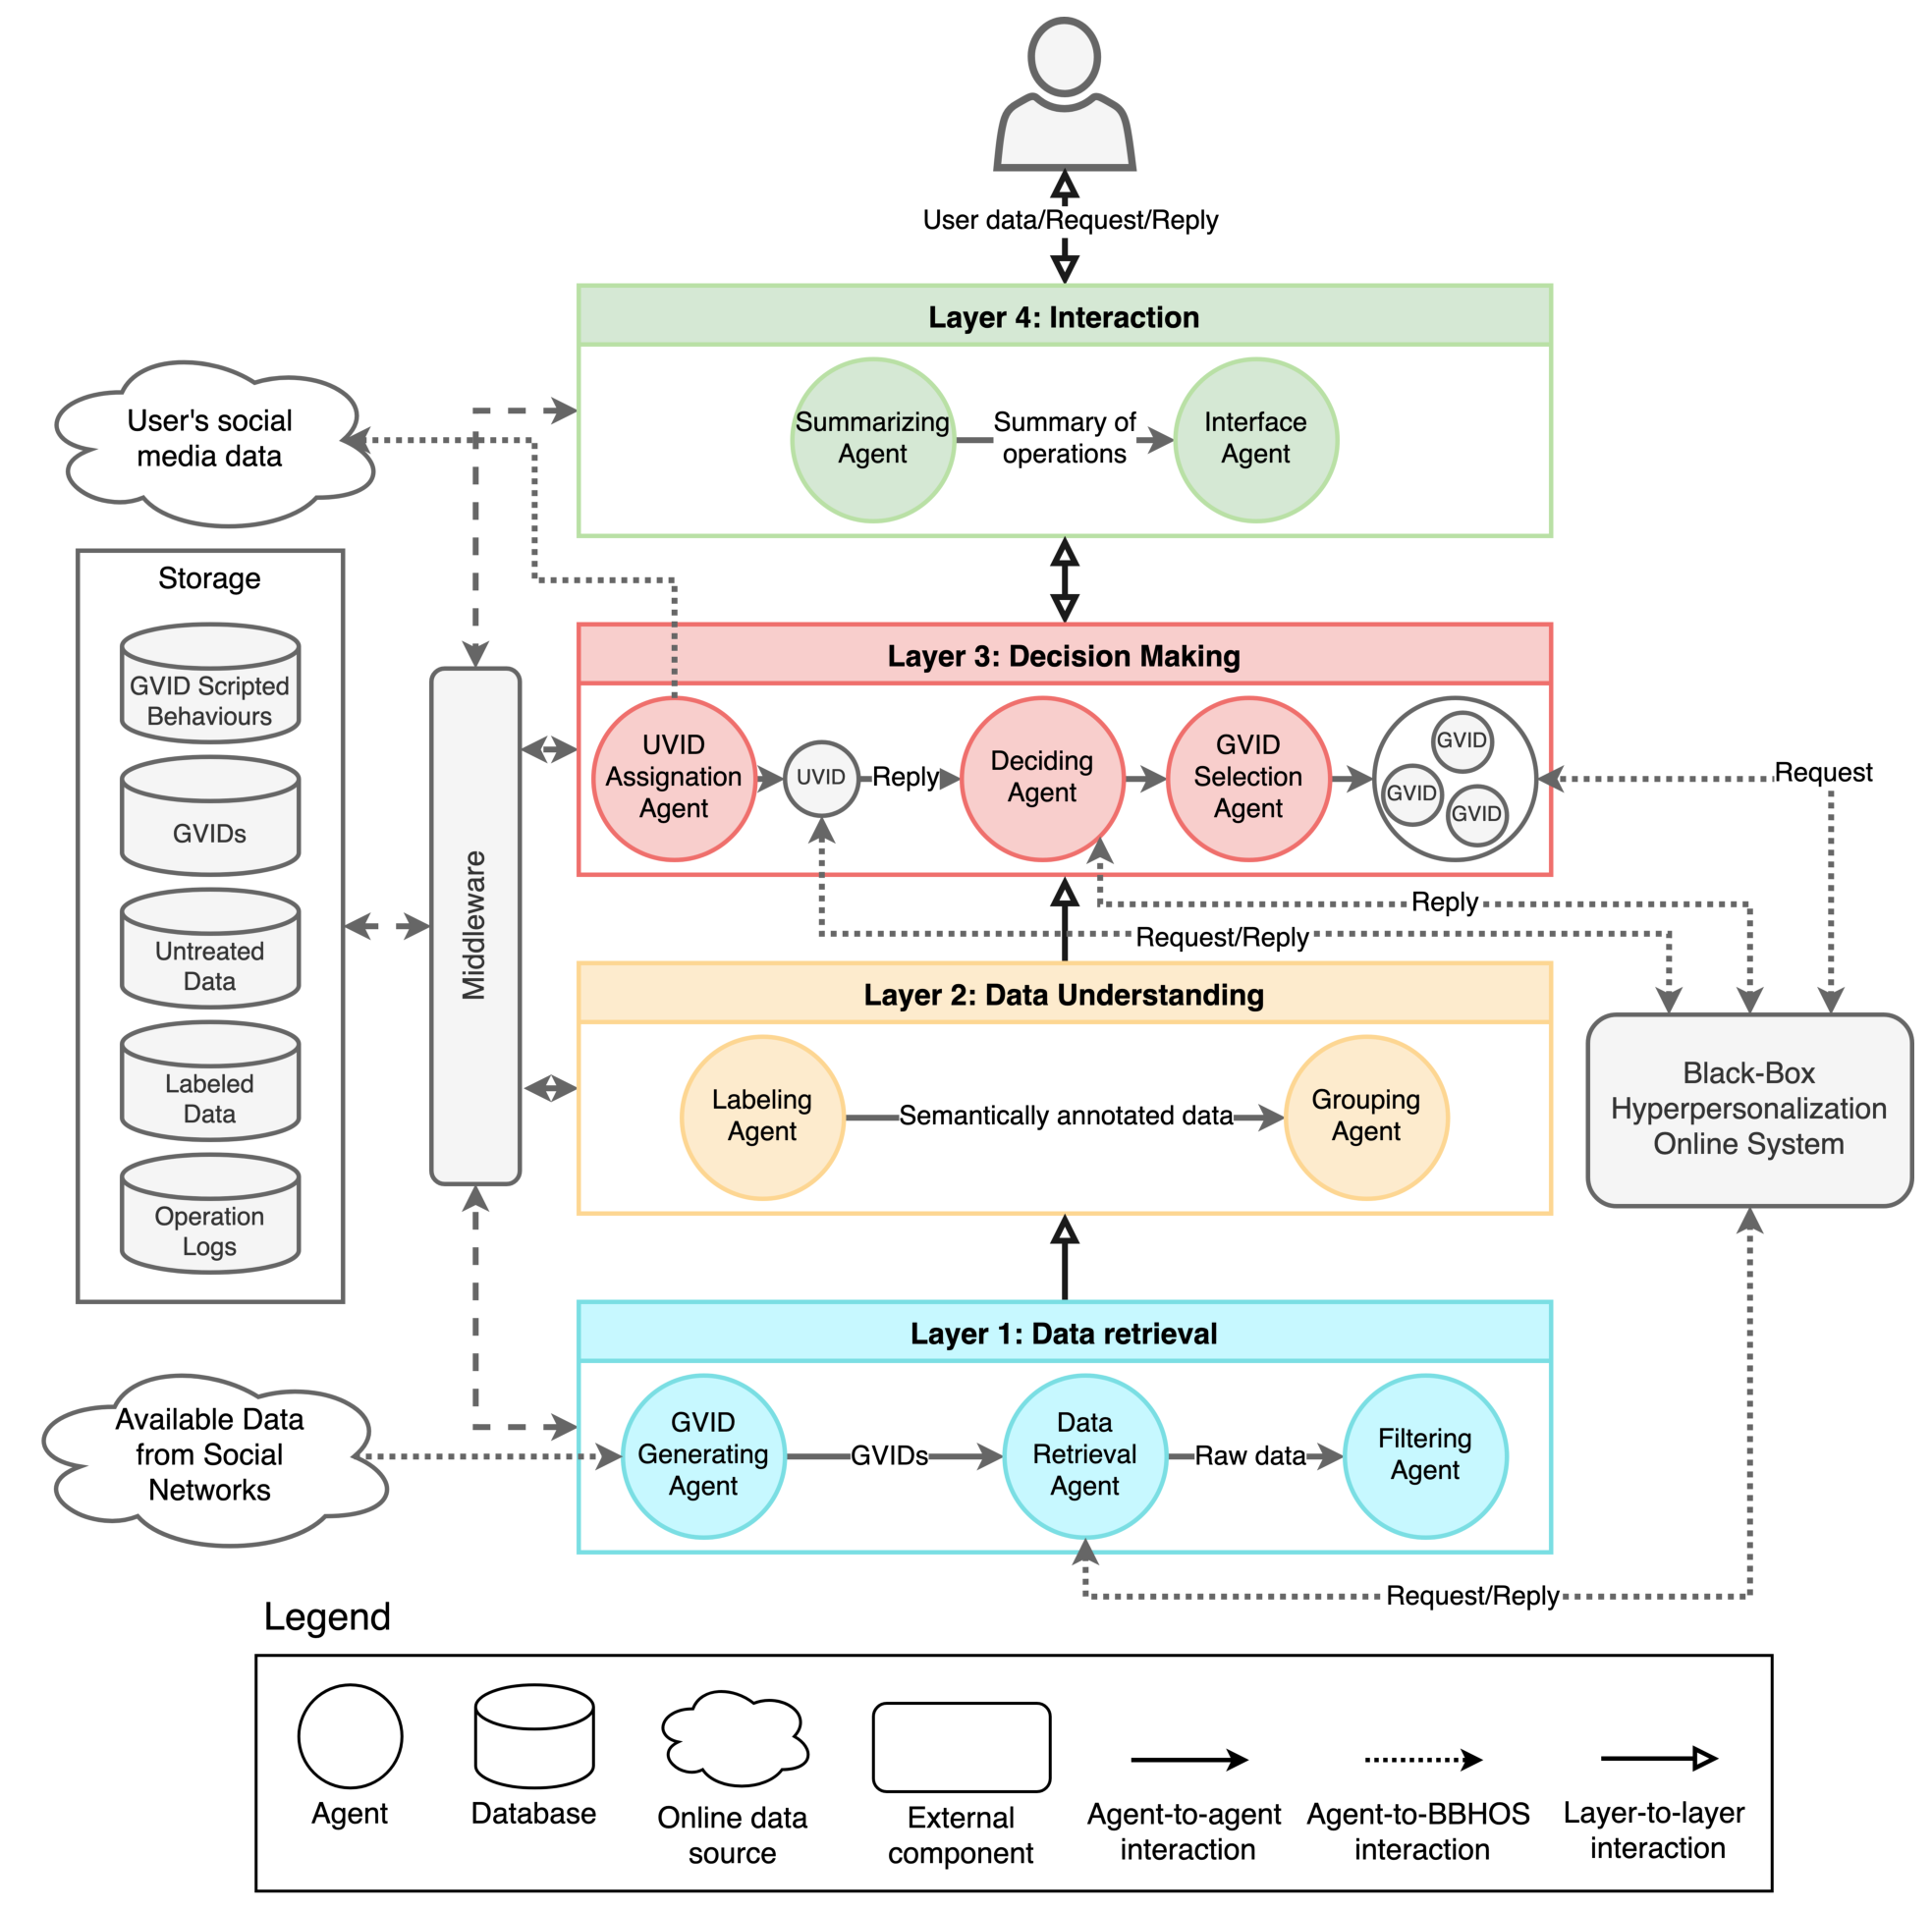
\includegraphics[width=.9\linewidth]{6_kbsextractiondl/figures/Overview_MAS.eps}
    \caption{Overview of the proposed hierarchical multi-agent system.}
    \label{fig:overview_mas}
\end{figure}

\subsubsection*{Layer 1: Data retrieval}
The first layer of the MAS comprises the operations related to the creation of GVIDs, as well as the BBHOS data extraction. This layer sets the purpose and goal of the system, selecting the BBHOS to study and the behavior of the GVIDs. Three agents can be identified in this layer:
\begin{itemize}
    \item \textit{GVID generating agent.} Two elements are considered by this agent to generate the GVIDs, providing them with unique features and enabling the realistic emulation of the behavior of real-life users. The first element are the core GVID features, which are stored in the system. These features include static treats such as gender, age, name, location, or interests. 
    
    Since static features are not enough to realistically emulate the behavior of a user, social media data is also scrapped to generate user profiles. This data is collected \textit{ad-hoc} from external sources and its not stored in the system. Natural Language Processing (NLP) techniques are used to analyze and extract relevant information from this data, such as topic modeling \citep{Alghamdi2015} or sentiment analysis \citep{sentimentanalysis}. Information such as preferences, opinions, or interests can be extracted from this data, which can then be added alongside the static traits of the GVIDs to generate more complex, human-like behaviors. GVIDs are stored, and subsequently used by the superior layers of the system. 
    
    \item \textit{Data retrieval agent.} GVIDs interact with the BBHOS by making requests and receiving responses, which are aligned with their features and behaviors. This agent orchestrates and supervises the interactions between the GVIDs and the services, collecting the data generated in the process. Data can have different different formats, according to the targetted BBHOS, ranging from plain text to video files. Collected data is stored for further analysis, as it can be used to redefine the static traits of the GVIDs.
    
    As BBHOS are online systems and are subject to network-related issues, which need to be corrected before transmitting the data to the next agent. Hence, this agent also performs operations such as duplicate or corrupted data removal. 
    
    \item \textit{Filtering agent.} This agent receives the interaction data between the GVIDs and the BBHOS, and classifies it according to its format (e.g., image, text, or audio). Filtering and homogenization operations are performed to extract relevant content from the received data and to facilitate the usage of data understanding processes. According to the data format, suitable filtering operations may be required, such as normalization or text preprocessing. This agent only considers formal aspects of the content.
\end{itemize}

\subsubsection*{Layer 2: Data understanding}
Data understanding processes are needed to extract knowledge from the outputs of the interactions between the GVIDs and the BBHOS. The second layer of the MAS deals with the procedures required for this task. General knowledge on the behavior of the BBHOS can be inferred from the analysis of the content fed to each particular profile (encoded on the GVIDs). Two agents comprise this layer:
\begin{itemize}
    \item \textit{Labelling agent.} This agent annotates, classifies, and extracts knowledge from the collected interaction data. Due to the heterogeneity amongst data types, suitable approaches are required to effectively extract knowledge from the unstructured data. Multi-label classification using Convolutional Neural Networks (CNNs) \citep{He2015DeepRL,CNNRNN} can be used for image treatment, detecting the elements included in an image. CNNs can also be used for audio and video classification \citep{HersheyCEGJMPPS16}. For further processing, audio can be transcribed \citep{speechrecognition} to enable text operations. 
    
    The majority of the responses generated by the BBHOS are textual, thus requiring a more profound analysis than the aforementioned data formats. Multiple NLP techniques can be considered to analyze textual data from distinct perspectives. Text classification techniques \citep{MIRONCZUK201836} may be suitable to categorize the retrieved content. Topic modelling \citep{pmlr-v15-nallapati11a,Alghamdi2015} enable finer-grained classification and content analysis. Additionally, document clustering, as well as text summarizing techniques \citep{Neto00documentclustering,YOUSEFIAZAR201793,Oikonomakou2005} can be used to simplify and group the data, facilitating its comprehension.
    
    The annotated data is then stored in the system. As most of the state-of-the-art approaches for the aforementioned tasks rely on deep learning models, periodical retrainings may be needed to keep the models updated.
    
    \item \textit{Grouping agent.} While BBHOS are opaque, associative patterns may be inferred based on the responses provided to each particular GVID. Furthermore, GVIDs can be grouped based on the similarity of their targeted responses. This agent establishes GVID aggregation based on this information, using a hierarchical approach ranging from specific to general. Therefore, heterogeneity between the lower level clusters is maintained, while converging into a single aggregation in the final top level. GVID aggregations are stored in the system.
\end{itemize}

\subsubsection*{Layer 3: Decision Making}
In this layer, the user's data input is collected, processed, and sent to the final interaction layer. While the previous two layers follow a forward-only criterion, where the data flows from inferior to superior layers, this layer has a bidirectional flow. This layer can therefore be considered the core element of the system, and its execution is triggered directly by the user. This layer comprises three agents:
\begin{itemize}
    \item \textit{UVID assignation agent.} This agent creates and deploys a virtual identity that represents the real user within the system, referred to as the \textit{User Virtual Identity} (UVID). The UVID serves as an intermediary between the BBHOS and the user, protecting the user from potential privacy invasions. Similarly to GVIDs, the static information provided about the user is complimented with available social media data, whose recollection must be approved by the user. Moreover, the UVID also encodes the user's specifications on the content, thus serving as a filter. 
    
    \item \textit{Deciding agent.} Once the UVID is deployed, it interacts with the BBHOS. If the retrieved content meets the user's specifications, the response is then transferred to the superior layer, where the user can approve it. If not approved, this agent passes this information to the \textit{GVID selection agent}, which querys the BBHOS generating a new set of responses. This agent is aware of the user's requirements and decides which, if any, of the returned responses are suitable. If there are no valid responses, this agent reenacts the query to the BBHOS to receive new responses. This process is iteratively performed until the user indicates the validity of the response, or until no GVID aggregations remain.
    
    This agent orchestrates the interactions between the GVIDs and the BBHOS and collects the information from the real user and distributes it to the following agent. The data generated by this agent is also stored for further analysis.
    
    \item \textit{GVID Selection Agent.} If the response received by the UVID does not satisfy the user requirements, new responses are required as shown in Figure \ref{fig:overview_mas}. A new GVID set is selected if the \textit{deciding agent} sends a negative response. Since a specific-to-general approach is considered, similar GVID aggregations are first selected. If the user professes a strong rejection on the previous BBHOS response, then the agent may select a polar opposite GVID set in the following iteration.
    
    The initial GVID set is selected according to the similarity between the UVID and the existing GVID sets. As GVIDs are arranged hierarchically, a nearest neighbour criterion can be used. Thus, the aggregation containing the most similar GVID to the UVID is selected in the first place.

    \begin{figure}[t]
        \centering
        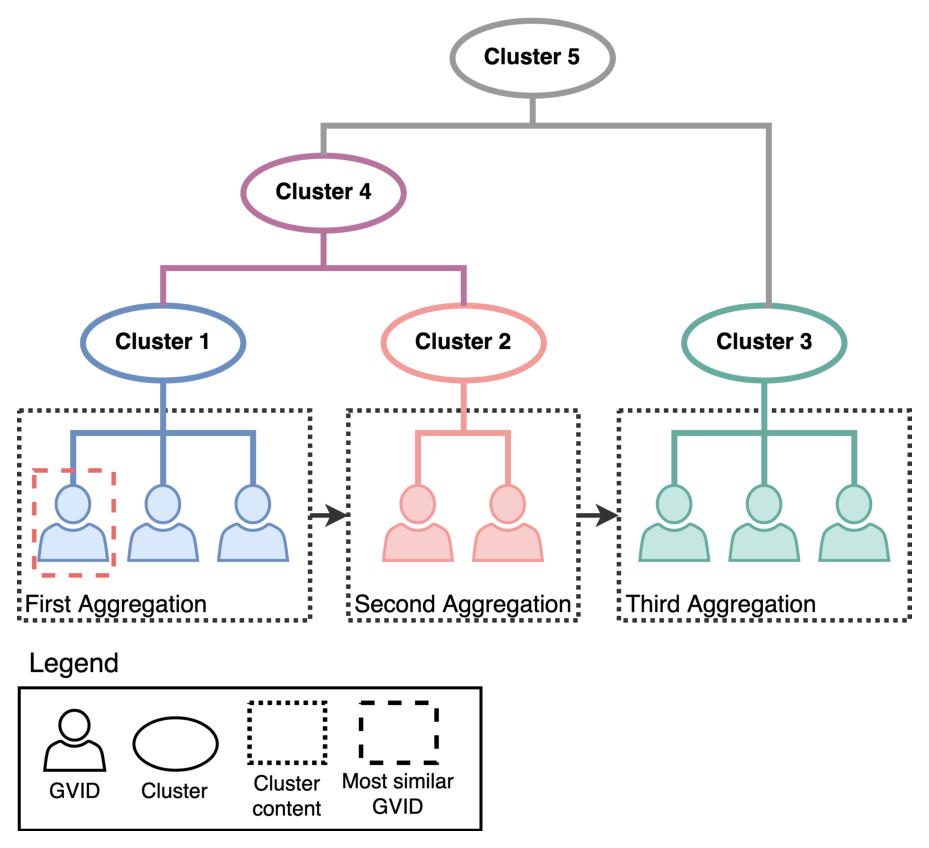
\includegraphics[width=.65\linewidth]{6_kbsextractiondl/figures/GVID_clusters.eps}
        \caption{Example of the GVID selection procedure.}
        \label{fig:gvid_selection}
    \end{figure}
    
    Figure \ref{fig:gvid_selection} depicts the general selection procedure. The GVID with the highest similarity to the UVID belongs to \textit{cluster 1}. Therefore, \textit{cluster 1} is selected as the initial GVID set. Then, the superior level of the hierarchy is explored (\textit{cluster 4}), which is composed of clusters 1 and 2. As \textit{cluster 1} has already been selected, \textit{cluster 2} would be selected as the next GVID aggregation. If the user does not express a strong disagreement with the provided responses, the system follows the specified hierarchical order to select the following aggregations.
\end{itemize}

\subsubsection*{Layer 4: Interaction}
Finally, an interaction layer is included to present the result of the operations performed in the inferior layers to the user. The data flow in this layer is also bidirectional, as the user not only receives, but introduces information in the system. User input is key to the system, as it conditions its behavior. The agents of this layer determine what and how the content is displayed to the user. They also collect input from the user and forward it to the inferior layers.

\begin{itemize}
    \item \textit{Summarizing agent.} To maintain the system's transparency, both the output and the log of the operations required for its generation are provided to the user. This agent extracts the logs of the iterations required by the \textit{deciding agent} to reach its final reply, and summarizes the most relevant information. Alongside the output, this agent generates a simple, user-readable record on which GVID received each response, as well as how many iterations were required. Thus, the real user can be conscious of whether the final response was obtained by the UVID or a different user profile (GVID).
    
    \item \textit{Interface agent.} User input is essential for the behavior of the system at its superior level. Appropriate mechanisms to interact with the user and correctly fulfill their requirements are needed. The communication with the user is established bidirectionally, implying that the system not only collects the user's input, but also generates an output that must be clear and readable. Therefore, this agent serves as a direct intermediary between the user and the system. The user's input is collected and transmitted to the lower layer for processing. Besides, this agent receives the output from the \textit{summarizing agent} containing the final BBHOS response and operation logs. This content is then displayed to the user in a simplified and visual format.
\end{itemize}

\subsubsection*{Storage units}
As depicted in Figure \ref{fig:overview_mas}, storage units serve as a sharing point for all MAS layers. The data generated during the system execution is heterogeneous, coming from different sources and in different formats. Five distinct databases are set to suit the different data types generated within the system:
\begin{itemize}
    \item \textit{GVID scripted behaviors.} Unique features are required to create a variety of user profiles to analyze the behavior of BBHOS. These features refer to mid-term information, such as interests or age, which remains static throughout the execution.
    
    \item \textit{Untreated data.} This unit stores data extracted from the interactions between the GVIDs and the BBHOS in the first execution stages. The responses obtained from the BBHOS can then be used to redefine the behavior of the GVIDs.
    
    \item \textit{Labeled data.} Once untreated data has been filtered, categorized, and annotated is stored in this database. This data can then be used to periodically retrain the models in the \textit{labeling agent} to keep the system updated. 
    
    \item \textit{GVIDs.} GVIDs are at the core of the system and used by multiple agents of the system across different layers. Therefore, it is critical to ensure their persistence and accessibility. As well as the single GVIDs generated in the first layer of the system, the aggregations obtained after performing hierarchical clustering is also stored within this unit. If there is a change in the GVIDs, a reaction to the \textit{GVID generating agent} is unchained, initiating the execution of the autonomous level of the MAS.
    
    \item \textit{Operation logs.} A log of the communications between the GVIDs and the selected BBHOS is saved. The data generated from these interactions enables the extraction of associative patterns that enable understanding over the BBHOS. These logs are generated in the third layer and used in the fourth for summarization.
\end{itemize}

Additionally, there is a \textit{middleware} between the databases and the agents that orchestrates and supervises the introduction and extraction of data from the different databases. The middleware also ensures data persistence and avoids concurrency issues.

\subsection{Data Flow}\label{6_sec:subsec:data_flow}

\begin{figure}[t]
    \centering
    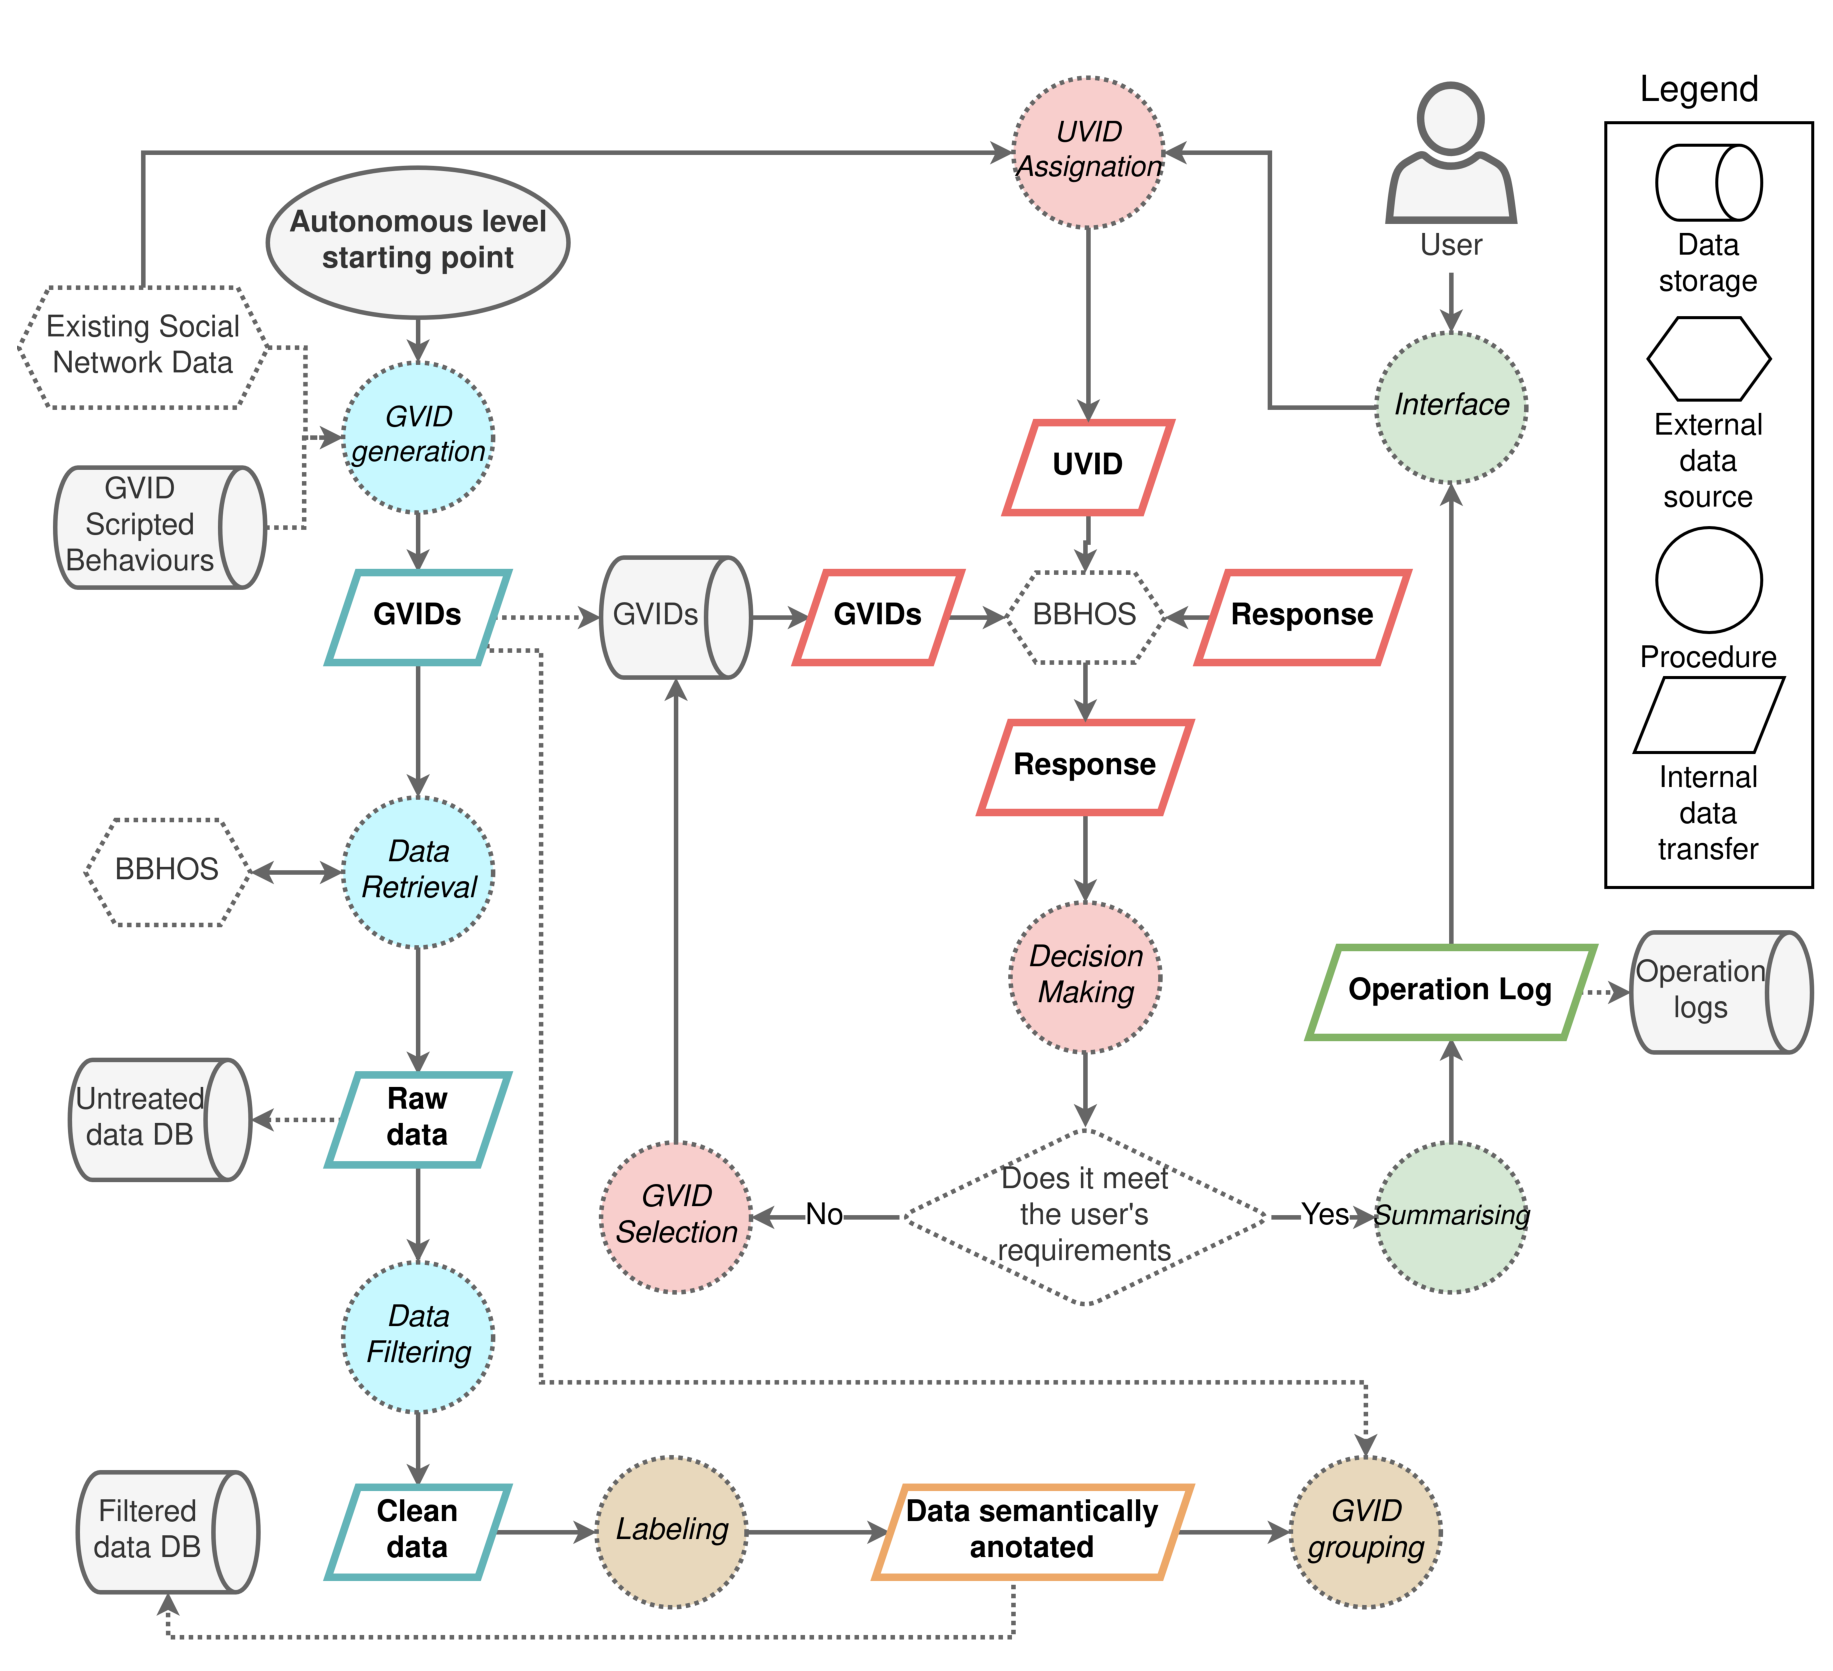
\includegraphics[width=\linewidth]{6_kbsextractiondl/figures/Data_flow.eps}
    \caption{Data flow of the proposed MAS. }
    \label{fig:data_flow_mas}
\end{figure}

Figure \ref{fig:data_flow_mas} depicts the data flow of the proposed MAS. Once the autonomous level of the system initiates, GVIDs are generated from a combination of scripted behaviors and existing social network data. The generated GVID set is then stored in the GVID database. GVIDs then interact with the BBHOS, receiving a set of responses in raw format, which are also stored for further analysis and GVID behavior correction. 

Response data at this stage remains untreated, containing both relevant and irrelevant information. This data is first classified according to its format into video, audio, image, and text to facilitate its annotation and analysis. Appropriate filtering and homogenization operations are performed on the data, according to its format. Images are resized and normalized, while markup and stopword removal is performed on textual data. Filtering and cleaning the data not only eases the annotation, but also considerably reduces its size. The models in the \textit{labeling agent} then annotate the filtered data and store it in its corresponding database. Hierarchical clustering is then performed to aggregate the GVIDs with respect to the content of their responses. GVID clusters are also stored in the GVID database.

The previous operations belong to the autonomous level and are subsequently executed without any user interaction. In the second level of the system, comprised by layers three and four, the user is the entry point, and its interaction with the system triggers its execution. The user accesses the system from the interface, specifying a set of goals and specifications. Then, the UVID is generated. The UVID then interacts with the BBHOS, receiving a targeted response. If this response meets the user's requirements, it is then summarized and forwarded to the user using the \textit{interface agent}. On the contrary, if the user rejects the response or it is not aligned to the specified requirements, a set of GVIDs are selected, repeating the same request over the BBHOS. Once the user agrees with a response, the user-triggered level of the system is suspended until further interaction.

\subsection{Case Study}\label{6_sec:subsec:case_study}


This Section presents a case study to illustrate the proposed architecture. This case study aims to provide a clearer and deeper insight on the interactions and data transfer between agents, giving a complete overview on the behavior of the system. 

\begin{figure}[t!]
    \centering
    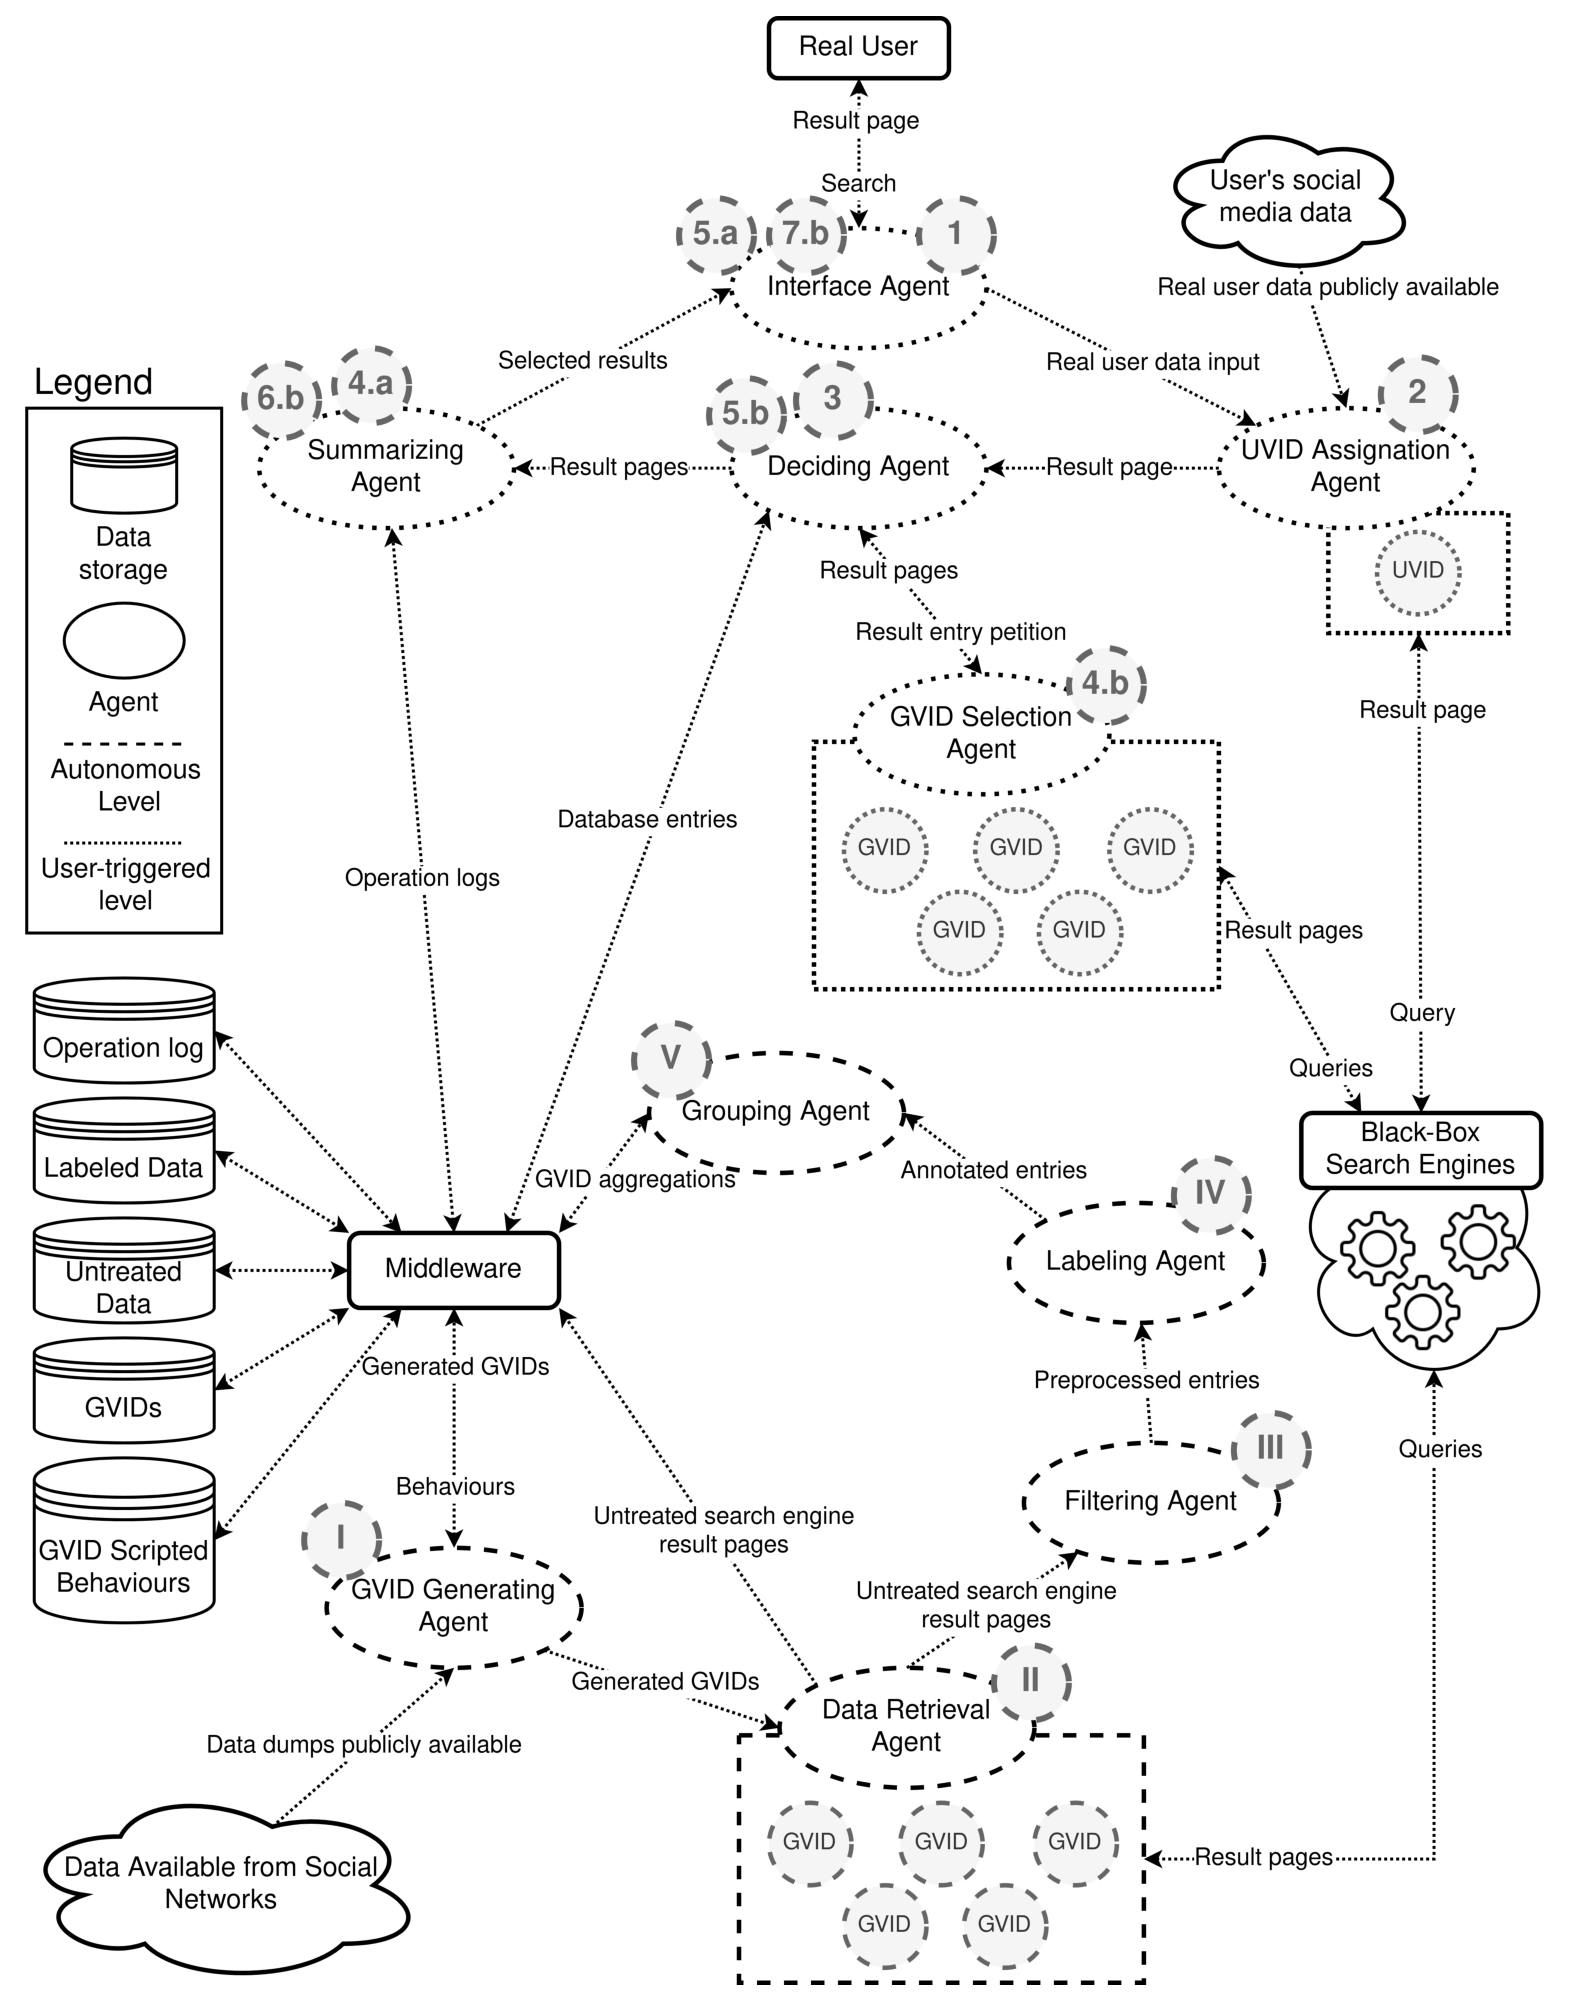
\includegraphics[width=.9\linewidth]{6_kbsextractiondl/figures/Use_Case.eps}
    \caption{Use case of the proposed architecture.}
    \label{fig:mas_use_case}
\end{figure}

The case study focuses on the analysis of the behavior of search engines. Specifically, on the relevance of the entries on the first result page. From the perspective of the user, the results that best fit the search query should be featured on the initial result page, independently from the employed search engine. However, this statement is not consistently met across search engines as the result may vary not only between search engines, but also between users. Moreover, most search engines feature advertising content amongst the top results, even when this content is unrelated to the search query. Therefore, this content should be detected and replaced by relevant result entries.

The considered case scenario meets the following specifications:
\begin{itemize}
    \item The goal of the system is to detect, analyze, and optimize result entries in search engines.
    \item Multiple search engines are selected, acting as the BBHOS.
    \item A reduced set of GVIDs is selected. Each GVID has distinct features to maximize heterogeneity in the BBHOS results.
    \item The system determines which results are related to the user's query, removing those entries that contain unrelated content, such as adverts.
\end{itemize}

As the architecture is divided into two distinct levels, the interactions between the agents on each level are presented separately. Figure \ref{fig:mas_use_case} illustrates the present use case. Operations related to the autonomous layer are numbered using Roman numerals, while Arabic numerals denote the operations user-triggered layer. Two distinct scenarios can occur based on the outcome of the \textit{deciding agent}, identified with letters \textit{a} and \textit{b} to designate the execution order of the agents.

\subsubsection*{Autonomous level}
In this level, the system gathers data from different search engines to be processed by the agents. The workflow is as follows:

\begin{enumerate}[label=\Roman*.]
    \item The \textit{GVID generating agent} collects the available social network user data dumps and extracts a set of \textit{N} GVID behaviors from the database. The collected social network data is then shuffled and distributed into \textit{N} different sets, each containing information such as tweets, reviews or opinions. Sentiment analysis and topic modeling are then performed over the sets to extract interest and opinions. This information is then combined with the GVID scripted behaviors to generate the final GVID set. The generated GVIDs are then stored in the database.
    
    \item Once the GVIDs are created, the \textit{data retrieval agent} selects a set of search engines to act as BBHOS, as well as defining the browsing terms to be queried. The browsing term set is composed by the topics extracted in the prior step. Each GVID does the same number of searches, and multiple GVIDs query the same term across the different engines. This enables the analysis of the results returned when the same term is browsed on different search engines and those obtained by different GVIDs when the search terms and engine are the same. The obtained responses are stored in the corresponding database.
    
    \item The result pages received by the GVIDs are then forwarded to the \textit{filtering agent}, which performs the data preprocessing. The collected data is in HTML format, thus containing several moot elements, such as markup text, references or symbols. The following operations are performed to clean the raw result pages: entry extraction, HTML and JavaScript markup removal, empty word removal and non-alphanumeric character removal. A set of clean result entries is obtained as outcome.
    
    \item As previously stated, search engines tend to merge advertising and valid result entries within the same page. Invalid entries should be detected and discarded, such that the user is only presented with entries that correspond to valid search results. The \textit{labeling agent} receives the result entry set from the previous agent and classifies entries into real result and advertisements. This problem can be subsequently treated as binary text classification. Labeled result entries are stored in the labeled data storage.
    
    \item Finally, GVIDs are hierarchically aggregated by their result entries to further analyzed the behavior of the search engines. The \textit{grouping agent} receives labeled entries and aggregates them following a hierarchical approach. As a result, GVIDs are grouped based on the result entries provided for each of them by the different engines. Information about the behavior of the search engines can then be extracted, such as which profiles are the most prone to receive advertising content, which engine includes the least amount of irrelevant content amongst its entries, or whether the results provided by the same engine on the same search vary across GVIDs. GVID aggregations are also saved in the GVID database.
\end{enumerate}

\subsubsection*{User-triggered level}
Once the autonomous level finishes its execution, the system remains suspended until a user makes a request. In this example, the request is a search query that the user inputs into a search engine. When the user makes the request, the user-triggered level of the system initiates its execution:
\begin{enumerate}
    \item The \textit{interface agent} collects the user's query, alongside with the needed user information. This input is sent to the \textit{UVID assignation agent} for further processing.
    
    \item The user's virtual identity, or UVID, is generated from the contextual information of the user, alongside with the publicly available social media information. The same procedure followed to generate the GVIDs is employed to generate the UVID. The UVID makes the user's search request, hindering the search engine from extracting contextual information about the user that could result in a privacy breach or lead to unfitting responses.
    
    \item The UVID executes the user's search query on the search engine. Then, the \textit{deciding agent} receives the result pages, determining whether the entries returned by the engine fit the user's request. Result entries are extracted from the result page to analyze their validity. These entries are filtered following the same procedure from step III. Then, the text classification model is used to discern advertisements from real result entries. At this point, two different scenarios can occur based on whether the result entries are real results (\textit{Scenario A}) or not (\textit{Scenario B}). 
    
    \paragraph{Scenario A}
    \begin{enumerate}
        \item [4.a] If the results provided by the engine to the UVID are relevant, meaning that no advertisements have been detected within the entries, the \textit{summarizing agent} compiles them for the user (e.g., removes duplicate entries).
        
        \item [5.a] Finally, the \textit{interface agent} builds a result page from the final result entry set and displays it to the real user. The constructed result page is formatted employing an adequate layout to present the information to the user in a clear and comprehensible way.
    \end{enumerate}
    
    \paragraph{Scenario B}
    \begin{enumerate}
        \item [4.b] If there is unrelated content amongst the results, the \textit{deciding agent} discards those entries and makes a petition to the \textit{GVID selection agent} to obtain new, valid entries to replace the removed ones. A set of GVIDs is selected following the hierarchical selection criteria, repeating the same query on the search engine. The new responses are sent back to the \textit{deciding agent}.
        
        \item[5.b] The new set of entries obtained by the GVIDs is analyzed by the \textit{deciding agent}, following the procedure presented in the step 3. The results that better fit the search query are then selected to replace the discarded entries. If no relevant results are found, the agent makes a new petition to the \textit{GVID selection agent}, repeating the process until valid result entries are obtained.
        
        \item [6.b] The generated result entry set, composed by the entries received by the UVID and the GVIDs, is transferred to the \textit{summarizing agent}. Aside from summarizing the result entries, this agent also generates a log comprising the operations required to obtain the final result entry set, identifying the GVID that originated each result.
        
        \item [7.b] The \textit{interface agent} composes a result page from the final entry set and displays it to the user, finishing the execution of the user-triggered layer of system.
    \end{enumerate}
\end{enumerate}

\subsection{Design Compliance}\label{6_sec:subsec:mas_design_compliance}
Section \ref{6_sec:mas_bbhos_general} introduces a hierarchical multi-agent system to extract behavioral patterns and improve user privacy in BBHOS, powered by DL. Figure \ref{fig:compliance_mas_extra_dl} depicts the specific design parameters of the presented use case:
\begin{figure}[t]
    \centering
    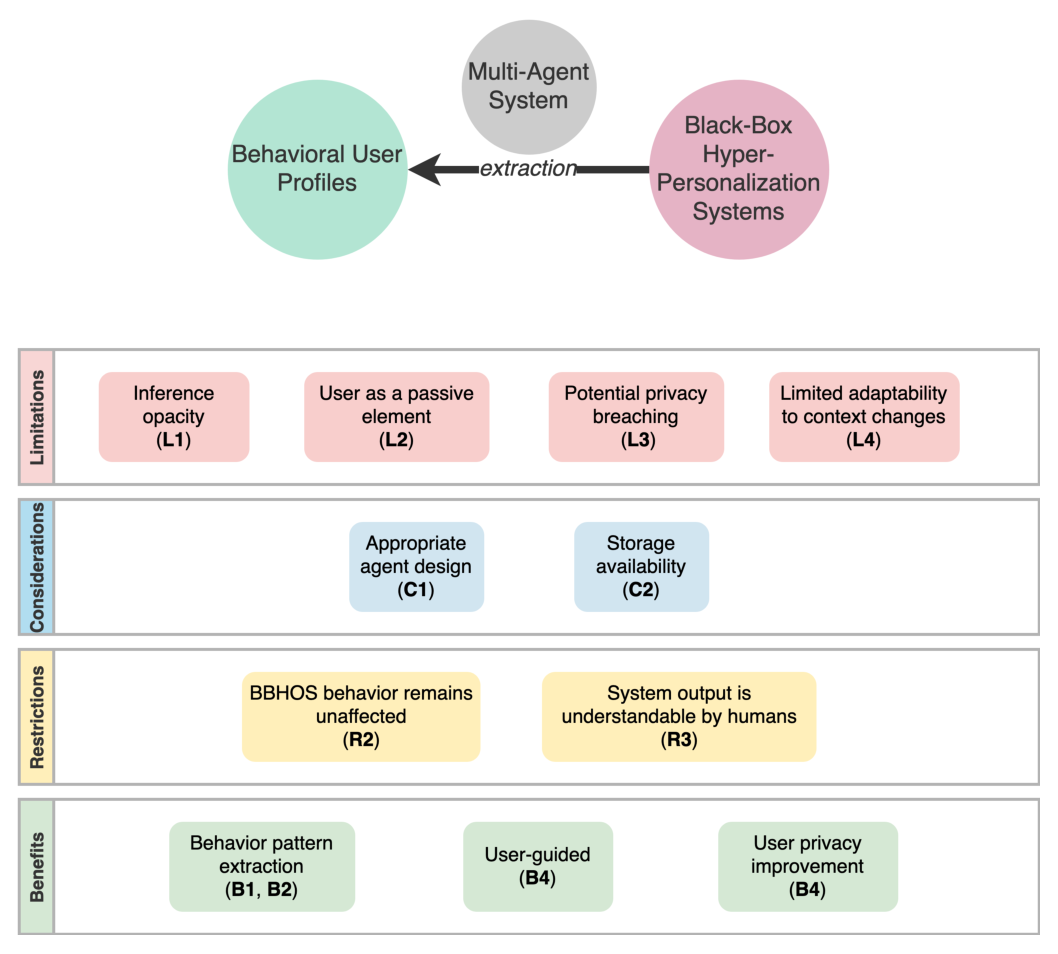
\includegraphics[width=\linewidth]{6_kbsextractiondl/figures/Instance_MAS_K_extraction_DL.eps}
    \caption{Overview of the design parameters of MAS extraction on BBHOS. In bold, the general design parameters as depicted in \ref{fig:kbs_extra_dl_overview}.}
    \label{fig:compliance_mas_extra_dl}
\end{figure}

\subsubsection*{Limitations}
\begin{itemize}
    \item \textbf{Inference opacity.} BBHOS are opaque by default. From a user perspective, the unawareness of why a content is targeted may prevent trust building. From a technical standpoint, opacity hinders the transferability of the model (\ref{kbsextradl_L_opacity}).
    
    \item \textbf{User as a passive element.} Even though the user is the core element of personalization, their role in BBHOS is entirely passive. The user is targeted on personalized content, but not actively inquired on its appropriateness. Instead, it is devised based on data that is collected unknowingly from the user (\ref{kbsextradl_L_human}).
    
    \item \textbf{Potential privacy breaching.} BBHOS rely on user-generated data to generate personalized, targeted content. While the user may initially give consent to provide their data, they may not be aware of its implications. Such is the case of microphone-collected data, where the user may not be conscious of being recorded, and subsequently can feel its privacy invaded when the BBHOS provides recommendations based on this data (\ref{kbsextradl_L_ethical}).
    
    \item \textbf{Limited adaptability to context changes.} BBHOS systems rely entirely on input data. This data is heterogeneous, reflecting diverse information. Some of this information may be actually relevant and reflect a change in the user context, while other may be misleading and induce noise into the BBHOS (\ref{kbsextradl_L_transferability}). 
\end{itemize}
\subsubsection*{Considerations}
\begin{itemize}
   \item \textbf{Appropriate agent design.} One of the main challenges in multi-agent systems is the agent design. In this scenario, the goal is to extract behavior patterns of BBHOS about their interactions with users and use them to improve the user's privacy and provide a better output. Agents must be devised to pursue this goal, thus ensuring that human-like behaviors are correctly emulated and accurate behavioral profiles can be extracted (\ref{kbsextradl_C_paradigm}).
    
    \item \textbf{Storage availability.} The proposed architecture comprises several storage units, each dedicated to a specific outcome. The storage capacity required may increase with subsequent system executions. Therefore, the availability of sufficient storage capacity must be guaranteed (\ref{kbsextradl_C_resource}).
\end{itemize}
\subsubsection*{Restrictions}
\begin{itemize}
    \item \textbf{BBHOS behavior remains unaffected.} One of the goals of the proposed MAS is to analyze the behavior of the BBHOS. Therefore, the BBHOS must remain unchanged to extract accurate insights and behavior patterns, as behavioral modifications can lead to inaccurate and erroneous conclusions (\ref{kbsextradl_R_behavior}).
    
    \item \textbf{System output is understandable by humans.} The user is at the core of the proposed MAS, being the main beneficiary. The output of the system must be aligned with this criterion, and therefore should be readable and understandable by humans (\ref{kbsextradl_R_human}).
\end{itemize}

\subsubsection*{Benefits}
\begin{itemize}
    \item \textbf{Behavior pattern extraction.} Opacity is one of the main setbacks of BBHOS. One of the main benefits of the proposed MAS is the capacity of extracting behavioral patterns from these opaque systems, identifying how the personalized content changes across different profiles and contexts. Behavioral patterns may not be enough to fully explain the inference process of BBHOS, but can provide some insight (\ref{kbsextradl_B_interpretability}). Moreover, these patterns can evidence existing biases amongst the types of content provided to different profiles (\ref{kbsextradl_B_bias}).
    
    \item \textbf{User-guided.} While users portray a passive role in BBHOS, in the proposed MAS the user is an active impactful element. The user initiates the execution of the top level of the system, and its interaction with the system conditions the behavior of the agents (\ref{kbsextradl_B_human}). 
    
    \item \textbf{User privacy improvement.} The behavioral patterns obtained by the MAS not only serve understandability purposes, but can be used to improve the user's privacy. The user is masked with an agent, which serves as a surrogate and interacts with the BBHOS. This agent can be modified accordingly to the user's goals and specifications to get better outcomes while simultaneously preventing the BBHOS to extract unwanted user data. 
\end{itemize}
%\section{A Hierarchical Multi-Agent Architecture Based on Virtual Identities}
\section{Generating Explainations and Insights on Knowledge Graph Embedding Predictions}\label{6_sec:geni_main}
%\section{Design Compliance I}
In Section \ref{4_sec:ontointro_kgc}, the introduction of ontologies into \textit{knowledge graph embedding} (KGE) models was explored to boost performance. Rules were also presented as an alternative to ontologies for semantic initialization, due to their capacity of encoding explicit and static restrictions about the data. However, in the existing rule integration approaches, the focus is on enhancing the model performance for \textit{knowledge graph completion} (KGC). Subsequently, the interpretability properties induced by the inclusion of rules within the model are not exploited. Therefore, KGE model explainability still remains a challenging issue. This Section presents a model-agnostic explainability framework for explaining knowledge graph embedding predictions.


\begin{sidewaystable}
\resizebox{\textwidth}{!}{
\begin{tabular}{|c|c|c|c|c|c|c|}
\hline
\textbf{Proposal} & \textbf{Type}   & \textbf{Baseline KGE Model} & \textbf{Constraints source} & \textbf{Goal of the proposal}                                                         & \textbf{Interpretable} & \textbf{Proposal focus} \\ \hline
\makecell{AMIE+ \\ \citep{amie+}}            & Rule-extraction & None                        & KG Data                     & Mine a set of rules from the KG                                                       & Yes                            & Output                  \\ \hline
\makecell{RUGE \\ \citep{ruge}}            & KGE Model       & ComplEx                     & KG Data + KG embeddings     & Enhance KGE performance                                                               & No                             & Input                   \\ \hline
RuleRec \citep{rulerec}          & Rule-extraction & None                        & KG Data                       & \makecell{Improve the performance of \\ recommendation systems while providing \\ explainable results} & Yes                            & Output                  \\ \hline
SLRE \citep{slre}             & KGE Model       & ComplEx                     & KG Data                     & Enhance KGE performance                                                               & No                             & Input                   \\ \hline
SoLE \citep{sole}             & KGE Model       & ComplEx                     & KG Data                     & Enhance KGE performance                                                               & No                             & Input                   \\ \hline
\makecell{pTransE\\ \citep{ptranse}}          & KGE Model       & TransE                      & KG Data                     & Enhance KGE performance                                                               & No                             & Input                   \\ \hline
TARE \citep{tare}              & KGE Model       & ComplEx                     & KG Data + KG embeddings     & Enhance KGE performance                                                               & No                             & Input                   \\ \hline
IterE \citep{tare}            & KGE Model       & ANALOGY                     & KG Data + KG embeddings     & Enhance KGE performance                                                               & No                             & Input \& Output                  \\ \hline
RuLES \citep{ruLES}           & Rule-extraction & None                        & KG Data + KG embeddings     & Mine a set of rules from the KG                                                       & Yes                            & Input \& Output         \\ \hline
KALE \citep{kale}             & KGE Model       & Translation-based           & KG Data + external sources  & Enhance KGE performance                                                               & No                             & Input                   \\ \hline
RBox \citep{rbox}             & KGE Model       & Translation-based           & External sources            & Enhance KGE performance                                                               & No                             & Input                   \\ \hline
\cite{yoonetal}      & KGE Model       & Translation-based           & Non-declared                & Enhance KGE performance                                                               & No                             & Input                   \\ \hline
RLvLR  \citep{rlvlr}           & Rule-extraction & None                        & KG Data + KG embeddings     & Mine a set of rules from the KG                                                       & Yes                            & Input \& Output         \\ \hline
\makecell{HyperKG\\ \citep{hyperkg}}          & KGE Model       & Translation-based           & KG Data                     & Enhance KGE performance                                                               & No                             & Input                   \\ \hline
RPJE \citep{rpje}              & KGE Model       & Translation-based           & KG Data                     & \makecell{Enhance KGE performance and \\ improve its interpretability}                              & Yes                            & Input \& Output         \\ \hline
\makecell{AnyBURL\\ \citep{anyburl}}          & Rule-extraction & None                        & KG Data                     & Extract a set of rules from KG                                                        & Yes                            & Input \& Output         \\ \hline
UKGE \citep{ukge}             & KGE Model       & DistMult                    & Uncertain KG Data           & Enhance KGE performance                                                               & No                             & Input                   \\ \hline
\makecell{r-TransE\\ \citep{rtranse}}         & Hybrid Model    & TransE                      & KG Data + Embeddings        & \makecell{Integrate embeddings and rules\\ into a unified framework for \\ KG Completion}             & Yes                            & Input \& Output                  \\ \hline
\makecell{CrossE\\ \citep{crosse}}        & KGE Model       & Translational Models        & KG Data                     & Development of an explainable KGE Model                                               & Yes                            & Input \& Output         \\ \hline
\makecell{DRUM\\ \citep{drum}}          & Rule-extraction & None                        & KG Data                     & Extract a set of rules from KG                                                        & Yes                            & Input \& Output  \\ \hline  
\end{tabular}  
 \caption{An overview of the existing approaches that combine rule- and embedding-learning methods.}
\label{tab:rules_kg}
}
\end{sidewaystable}

Table \ref{tab:rules_kg} provides an overview of the existing hybrid models that integrate rule-based systems and KGE. CrossE \citep{crosse} is also included despite not using rules, as it is one of the few existing KGE models that explicitly considers explainability. Two tendencies can be detected among the models presented in Table \ref{tab:rules_kg}: rule mining and KGE performance boosting. The first tendency applies only to rule-learning models, where rule-learning takes the primary role. In these models, KGE supports the confidence validation and assessment of the extracted rules, as well as assisting in pruning and ranking. As rule-learning models aim to mine rules from the KG, their focus is not on the input data, but on the validation of the model's results.

\begin{figure}[t]
    \centering
    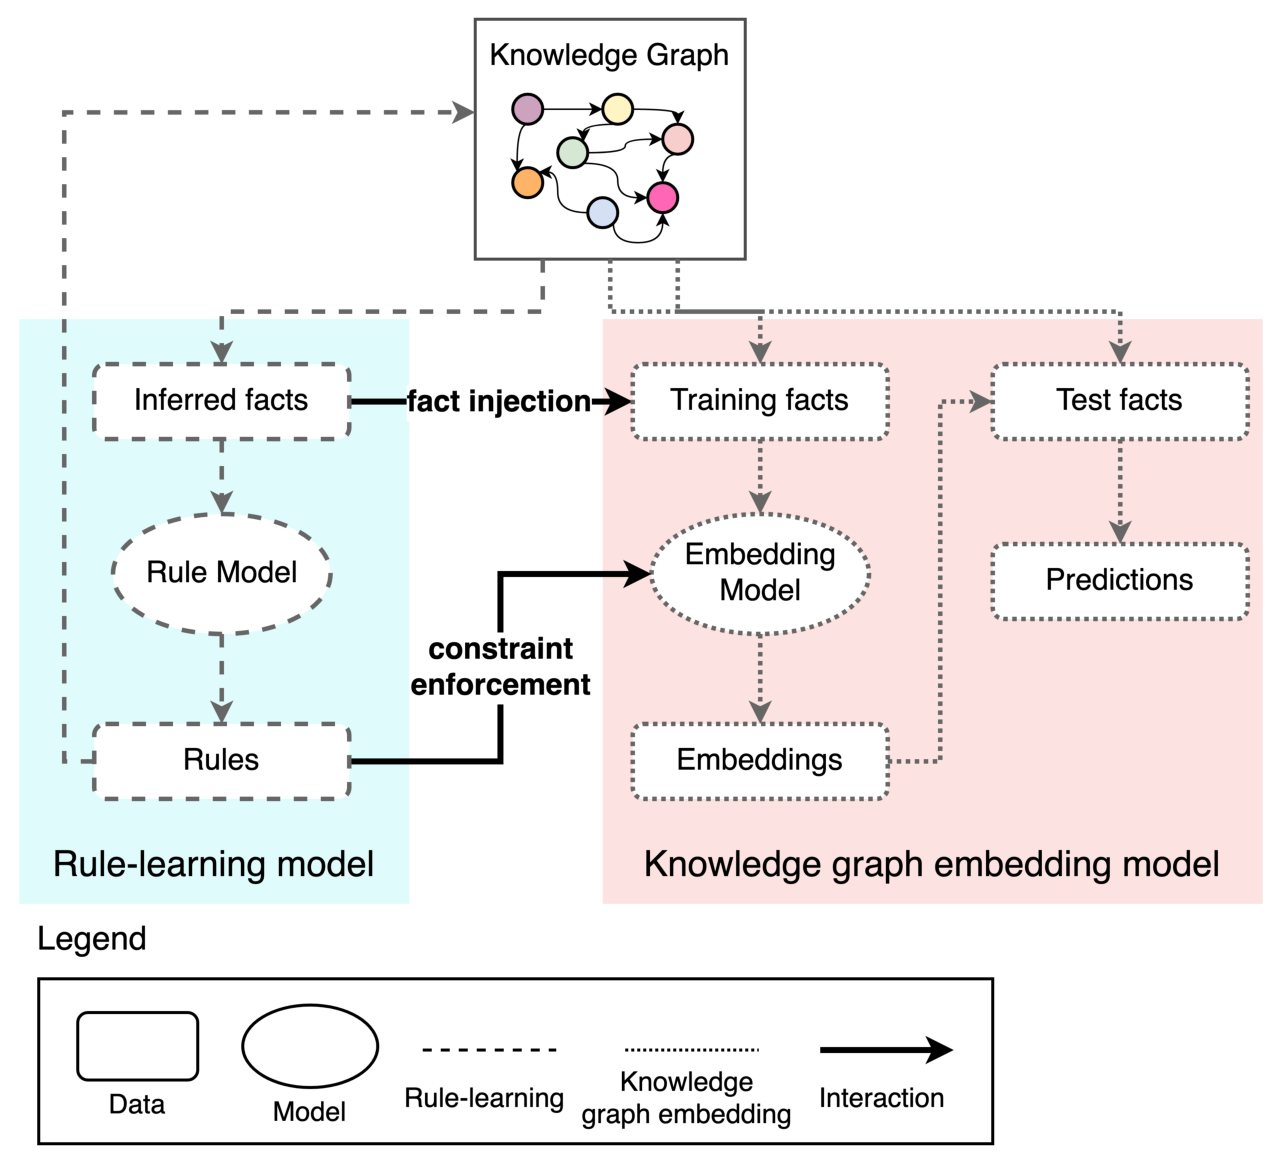
\includegraphics[width=.7\linewidth]{6_kbsextractiondl/figures/rule_support_training.eps}
    \caption{General workflow of a knowledge graph embedding model training with rule-based support.}
    \label{fig:rule_training}
\end{figure}

Several embedding-learning models incorporate rules as a supporting element to improve performance. In this scenario, the benefits of rule introduction are twofold: increasing the number of available training facts through rule instantiation and enforcing explicit constraints between relations. Furthermore, while rule-learning methods iteratively refine the results provided by the model, embedding-learning strategies focus on improving the input so that the improvements are propagated throughout the model and reflected in the final results. Figure \ref{fig:rule_training} depicts the general workflow of a rule-supported KGE model. As depicted, rules are only considered during model training. Therefore, the focus is on boosting the performance of the model instead of explaining the final predictions.

Data augmentation approaches rely on rule mining models, such as AMIE+ \citep{amie+}, to extract a set of rules from the KG. The generated rules can then be instantiated with the KGE training facts, leading to new facts. Increased data availability during training leads to improved final results. In those cases where the focus is on learning and imposing relation constraints, rules and restrictions are computed alongside the embeddings. Rules are then used to evaluate the consistency of the embeddings. The final embeddings encode rule restrictions, leading to better predictions.

As reported in Table \ref{tab:rules_kg}, only two of the studied KGE models are capable of providing interpretable results. This is directly related to the training paradigm of KGE models, where the goal is to improve the accuracy and performance of the model across different metrics. Moreover, most of the reported KGE enhancement proposals are only suitable for specific models, hindering its reusability.

\cite{bianchi_kge_explainability_2020} presents a study on the explainability of KGE models. As denoted in this work, defining explainability in this context is not trivial, as there is not an agreed definition. In the context of KGE, any potential information that can accurately relate the model prediction to both the input data and the embeddings can be regarded as an explanation. According to this definition, DistMult \citep{distmult} was one of the first attempts of introducing explainability in KGE models. In addition to providing a novel KGE proposal, DistMult also presents a method for the generation of Horn clauses from embeddings. Moreover, this work introduced a novel perspective on rule mining: replacing the KG with the embeddings as the data source. This change of paradigm not only solves one of the main issues in rule-mining models (search space optimization), but also provides a novel and data-agnostic vision on the subject.

\subsection{GEnI: A Knowledge Graph Embedding Model-Agnostic Framework}\label{6_sec:subsec:geni}
This Section introduces GEnI: a three-level, model-agnostic explainability framework. Following the guidelines established in DistMult, the first mainstay of the approach is that \textit{all insights on the inference process of the model should be extracted from the embeddings, not the data}. This criterion ensures that the proposal strictly explains the model output, and not the KG itself. This approach also relates the quality of feasible explanations to the performance of the KGE model. Therefore, if the model produces accurate predictions, GEnI may also provide an insight on the inference that leads to the output. On the contrary, if the KGE model has a subpar performance, no information on the output may be inferred. Aligned with this principle, the second mainstay of the proposal is that \textit{the KGE model output is considered as a ground truth to be explained, independently on its rightfulness.}

\begin{figure}[t]
    \centering
    \includegraphics[width=\linewidth]{6_kbsextractiondl/figures/geni_overview.eps}
    \caption{Overview of the proposed KGE explainability framework}
    \label{fig:overview_geni}
\end{figure}

Figure \ref{fig:overview_geni} showcases the general behavior of the framework. First, the KGE model generates a prediction on a given input fact. In the example, the KGE model is inquired about the fact \textit{(Madrid, capital of, ?)}, to which the provided response is \textit{Italy}. The framework then aims to provide an insight on why the fact \textit{(Madrid, capital of, Italy)} is inferred. The explaination process comprises three sequential phases, ranging from more general to more specific. 

In the first two phases, potential insights are extracted from a set of operations performed directly over the embeddings, which are then validated against the KG data. A criterion is established to decide which of the potential insights should be validated and presented to the user in case of success. From a general standpoint, insights are extracted by establishing a comparison between a given operation $O_p$ over the input fact and the results obtained from executing $O_p$ over the set of potential entities $\mathcal{E}'$ and relations $\mathcal{R}'$. Equation \ref{eq:general_restriction} draws the general restriction for insight extraction, where $|$ denotes the logical operator OR:

\begin{equation}\label{eq:general_restriction}
    Op(s,r,o)\approx [Op(\mathcal{E}') | Op(\mathcal{R}')]\,.
\end{equation}

Measuring the similarity between the results of the operations on both sides of the inequality is essential for extracting good insights. The elements of the equation can be either vectors or matrices depending on the phase and the KGE model. Therefore, different metrics are required to compute the similarity between both sides of the equation. Regarding vector operations, cosine similarity is the preferred choice, as it provides values in the range $[-1,1]$. For matrices, Frobenius norm is the standard comparison metric. However, since both metrics use different scales, as the Frobenius norm is a distance-based metric, Euclidean norm is used for vector comparison. 

Distance-based metrics are not bounded to a fixed range, which hampers the comparison between results. Moreover, the range of entity and relation embeddings depends on the KGE model, as well as on the initialization. A tolerance threshold is therefore specified to denote which is the maximum acceptable distance between two comparable components (matrices or vectors) to consider them similar. If the threshold value is too restrictive, no insights on the prediction may be found. Alternatively, low threshold values can lead to inaccurate insights while significantly increasing the computational time. The optimal threshold value can be empirically computed, but it must not be treated as a quantitative element, but a qualitative one. Therefore, the threshold value is specified by the user, introduced as a similarity value in the range $[0,1]$. This value is then rescaled and translated into the threshold $th\_value$ as follows:

\begin{align} 
   tolerance = max(\mathcal{G}_{embeddings})- min(\mathcal{G}_{embeddings}), \nonumber  \\
    th\_value = tolerance + ( 1 - sim\_ratio ) \times  tolerance,
\label{eq:threshold_value}
\end{align}

where $\mathcal{G}_{embeddings}$ is the values of all the embeddings (both entities and relations), and $sim\_ratio$ is the user-specified similarity ratio. Equation \ref{eq:threshold_value} ensures that the threshold value $th\_value$ is compliant with the embedding range and the similarity value specified by the user. Insight candidates are then filtered according to Equation \ref{eq:candidate_filter}:

\begin{equation}\label{eq:candidate_filter}
    dist( Op(s,r,o),  [Op(\mathcal{E}') | Op(\mathcal{R}')] ),
\end{equation}

where $O_p$ is the phase-specific operation and $dist$ the corresponding distance function (Euclidean or Frobenius). 

Similarly to rule-based models, efficiently traversing the search space to find the relevant elements is one of the key challenges. In rule-learning systems, search space optimization is performed using pruning and walking algorithms. However, these methods can not be applied in this scenario, where the search space is composed by a set of labeled embeddings. In rule-based models, axioms are mined from the detection of facts that share common elements, or whose relations feature similar entities. Although this criterion can not be directly applied to the proposed framework, an equivalent approach can be followed to compute related elements from the embeddings. Once trained, both entity and relation embeddings encode semantic information about their interactions with the graph components. KGE model training also ensures that entities and relations that have similar interactions lead to close embeddings in the resulting vector space. 
In the context of embeddings, search spaces can be envisioned as clusters generated under the aforementioned constraints. Therefore, elements with similar embeddings are grouped into the same cluster. Under this criterion, the search space for a given insight is composed of clusters of subject and object entities, as well as their predicates. Efficiently detecting these aggregations poses a considerable challenge, as the performance of most clustering approaches does not scale up with the dimension of the data. Both entity and relation embeddings have dimensions that exceed the hundred entries, which squares up for relation matrices. For high-dimensional data, operations such as principal component analysis may be required.

\subsubsection*{Phase 1: Axiom extraction from relation embeddings}

One of the core principles of the proposal, as previously stated, is that all explanations must stem from the embeddings, and not the data. Subsequently, embedding-based mechanisms capable of accurately extracting rules from the representations are required. IterE \citep{itere} presents the equivalence between OWL2 ontology axioms and their corresponding rule formulations. Seven axiom types are reported in the original work, but only five are considered in this proposal. The reflexive property is not considered, as KGs should not include self-loops, thus making this property unfeasible.  The sub-object property is also removed due to its redundancy with the equivalence property, as they both derive from the same rule form. Table \ref{tab:owl_restrictions} draws the relation between axioms, rule forms, and embedding restrictions in both translational and bilinear models. These models follow the scoring functions outlined in Section \ref{subsec:s4_theoretical_back}. While each KGE model introduces variations with respect to the baseline function, the generated embeddings are still compliant with the baseline scoring functions. These functions can then be used to infer general restrictions about the embeddings that are equivalent to the studied axioms, as outlined in Table \ref{tab:owl_restrictions}. These restrictions can be used to identify rules directly from the embeddings.

\begin{table}[t]
\resizebox{\linewidth}{!}{
\begin{tabular}{cccc}
\textbf{OP Axioms}      & \textbf{Rule Form}              & \makecell{\textbf{Bilinear}\\\textbf{Restrictions}} & \makecell{\textbf{Translational}\\\textbf{Restrictions}} \\
SymmetricOP($r$)          & $(y,r,x)\leftarrow(x,r,y)$                 & $M_r M_r \simeq I$                          & $v_r+v_r \simeq 0$                           \\
TransitiveOP($r$)         & $(x,r,z)\leftarrow(x,r,y),(y,r,z)$         & $M_r M_r \simeq M_r$                         & $v_r+v_r \simeq v_r$                           \\
EquivalentOP($r$)         & $(x,r_2,y)\leftarrow(x,r_1,y)$               & $M_{r_1} \simeq M_{r_2}$                         & $v_{r_1} \simeq v_{r_2}$                           \\
InverseOP($r_1,r_2$)        & $(x,r_1,y)\leftarrow(y,r_2,x)$               & $M_{r_1} M_{r_2} \simeq I$                        & $v_{r_2}+v_{r_1} \simeq 0$                         \\
ChainOP(ChainOP($r_1,r_2$),$r$) & $(x,r,z)\leftarrow(x,r_1,y),(y,r_2,z)$ & $M_{r_1} M_{r_2} \simeq M_r $                       & $v_{r_1}+v_{r_2} \simeq v_r$                        
\end{tabular}}
\caption{Relation of object properties with their corresponding rule forms. Inferred mathematical restrictions under the two KGE assumptions (Bilinear and Translational) are provided. $M$ and $v$ denote the relation matrices and vectors, respectively.}
\label{tab:owl_restrictions}
\end{table}

When a new fact $(s,p,o)$ enters the framework, the embedding of the predicate $p$ is retrieved. First, symmetry and transitivity are evaluated according to their restriction operations. The threshold value $th\_value$ is used to establish whether the inequality holds. If the restriction is met, the corresponding axiom is considered for further evaluation. The same process is followed for the remaining properties. Efficiently and accurately detecting which relations in $\mathcal{R}$ are the closest to $p$ is the main challenge of this phase. Usually, the number of relations in a KG is pretty limited. K-means can be used to detect neighbouring relations, where the optimal value of $k$ is computed via gap-statistic optimization. While k-means provides a simple and effective solution, it does not accurately capture the KG, as it only assigns a single cluster per relation. C-means poses a fuzzy alternative to k-means, based on the same aggregation criteria but considering the possibility that an element can belong to more than one cluster. Additionally, it can automatically estimate the optimal number of clusters. C-means is selected as the neighbour detection method for relations.

Once predicate $p$ is evaluated on all properties, a set of potential rules is obtained. At this stage, the rules are not instantiated, and subsequently it can not be ascertained whether the input fact can be inferred from them. Potential rules are then evaluated on the KG facts. In this evaluation, potential rules are instantiated to find a feasible inference for the input fact. If a valid instantiation, it is returned to the user and the execution finishes. Second phase is initiated if no rules or instantiations are found.

\subsubsection*{Phase 2: Correlation between predicates}
In the first phase, only the predicate is considered. The second phase also includes entity information, being an intermediate solution between the general information provided by rules and the specificity of influencial fact detection. 

For some facts, the information on the predicate $p$ may not be sufficient to generate an insight on the inference process, as none of the properties in Table \ref{tab:owl_restrictions} may be observed. However, when combined with either the subject or object entity representation, $e$, a degreee of similarity can be observed between the obtained representation and those obtained by performing the same operation on the relation set $\mathcal{R}$ and the subset of entities related to $e$ denoted as $\mathcal{E}'$.

In the previous phase, c-means was sufficient to detect neighbouring relations efficiently and accurately, due to the limited number of elements. For entities, c-means can be ineffective due to the elevated number of elements, which can lead to a high number of single-element clusters which do not comprise a valid search space. Agglomerating hierarchical clustering is used as an alternative in this phase. First, the pairwise distance matrix is computed, measuring the Euclidean distance between each possible pair of entities in $\mathcal{E}$. From this matrix, entities are then aggregated using an agglomerating criterion that prioritizes the maximization of elements within each cluster. The set of closely related entities $\mathcal{E}'$ for an entity $e$ is the entities contained in its own aggregation.

\begin{figure}[t!]
    \centering
    \subfigure[Direct Correlation \label{fig:direct_corr}]{\includegraphics[height=1.7in]{6_kbsextractiondl/figures/direct_corr.eps}}
    \qquad
    \subfigure[Triangular Correlation \label{fig:triangular_corr}]{\includegraphics[height=0.9in]{6_kbsextractiondl/figures/triangular_corr.eps}}
    \caption{Overview on the two types of predicate correlations.}
    \label{fig:corr_overview}
\end{figure}

Figure \ref{fig:corr_overview} depicts the two types of correlations that can be identified based on the interactions between $\mathcal{E}'$ and $\mathcal{R}$ for the input fact.

\paragraph{Direct correlation}
In some cases, the inference of a particular entity $e$ can be explained based on the existence of a \textit{(relation,entity)} tuple that frequently features not only $e$, but closely related entities in $\mathcal{E}'$. As depicted in Figure \ref{fig:direct_corr}, \textit{direct correlations} are a widespread occurrence in relation pairs such as \textit{born in} and \textit{nationality}, as people from a given country will most likely have the same nationality. In these scenarios, where a pair of predicates $(X,r_1,e_1)$ and $(X,r_2,e_2)$ frequently feature the same entities, the KGE model is likely to learn this correlation for future inferences.

The following operations are performed on an input fact $(s,p,o)$ to extract potential direct correlations. First, the embeddings of the relation $p$ and predicted entity $e$ ($s$ in subject prediction and $o$ in object prediction) are extracted. Then, the set of entities related to $e$, $\mathcal{E}'$, is retrieved. Each entity $e \in \mathcal{E}'$ is operated with each relation in $\mathcal{R}$ via addition (translational models) or multiplication (bilinear models). The result of this operation is a matrix $M$ with dimensions $E \times d$, where $E$ is the number of entities and $d$ is the embedding dimension. Entries in $M$ whose Euclidean distance to $p$ is equal or less than the threshold value $th\_value$ are considered as potentially direct correlations. 

The set of potential direct correlations is then evaluated on the KG, assessing whether the input fact can be inferred. In addition to providing insight on the inference of a given fact, detecting these correlations can also help identify data biases. Detecting and correcting these biases can improve the overall performance of the model.

\paragraph{Triangular correlation}

In \textit{triangular correlations}, the correlation is not established between pairs of tuples, but between a tuple and a single entity. Figure \ref{fig:triangular_corr} depicts an example of this correlation. This phenomenon is relatively common in cases with a lack of facts about the predicted entity $e$ during training. This correlation establishes that, when the number of facts containing the entity $e$ is limited, its representation can be replaced by the resulting embedding of operating its most related entity $e'$ with the relation $r'$ that links them.

Similar to direct correlation, the first step is to extract the set $\mathcal{E}'$ containing the entities closely related to $e$. Then, each entity $e' \in \mathcal{E}'$ is operated with the representation of the predicate $p$, generating a matrix $M$ of dimension $E \times d$. Those entries in $M$ whose Euclidean distance to $e$ is equal or less than the threshold value $th\_value$ are considered for evaluation.

In addition to the explainability provided by these correlations, their detection can also be used as an indicator of which entities are lacking information. Moreover, it can also boost KGE model training, as it indicates which triples may not be relevant and can therefore be removed from training. 

Detected correlations (triangular or direct) about the input fact are evaluated on the KG. If the evaluation succeeds, the system finishes its execution. 

\subsubsection*{Phase 3: Influential fact detection}
Phase 3 initiates, as illustrated in Figure \ref{fig:overview_geni}, when none of the previous two phases succeed. Instead of providing broad and general explanations that can be feasible for more than one fact, phase 3 generates insights that can only explain the given input fact. 

Influence functions measure the shift value of an estimator at a given point when a certain indicator changes. In the context of KGE, influence functions assess the impact that a fact has on a prediction. CRIAGE \citep{criage} presents an adaptation of the general influence function for its application to bilinear KGE models. CRIAGE uses the Taylor expansion to estimate the change in the score of a given fact by approximating the difference in the embeddings when a fact is added or removed. Equation \ref{eq:influence} defines CRIAGE variation on the baseline influence function, where $S(s,p,o)$ is the score of the fact $(s,p,o)$, $f$ denotes the model scoring function, $H_o$ is the Hessian matrix containing the second-order derivative of the loss with respect to the embedding of the object entity, and $\varphi$ is the sigmoid of the score.

\begin{equation}\label{eq:influence}
   \widetilde{S}(s,r,o)-S(s,r,o) = f_{s,r}[(1-\varphi){(H_o+\varphi(1-\varphi)f_{s',r'}^{T}f_{s',r'})}^{-1}f_{s',r'}^{T}].
\end{equation}

The goal of CRIAGE is to evaluate the robustness of a KGE model, assessing the impact of added and removed facts on its performance. Therefore, the goal is not to detect how the predictions change which are the most influential facts on a given prediction, but to evaluate the overall behavior of the model when the training set changes. On the contrary, the proposed approach focuses on the effect a fact $f'$ has on the prediction of the input fact $f$ when removed. The more significant the shift in the score of $f$, the more impact $f'$ has on its prediction. The influence function proposed by CRIAGE is also extended to cover translational models.

The first step is to detect which fact or set of facts $\mathcal{F}'$ has the bigger impact on $f$. Facts in $\mathcal{F}'$ are those that either the subject or object entity with fact $f$. In this case, the set of related facts $\mathcal{F}'$ cannot be extracted using unsupervised learning. Once $\mathcal{F}'$ is computed, the shift of score in $f$ for each fact $f' \in \mathcal{F}'$ is evaluated using Equation \ref{eq:influence}. Those facts that cause a shift that switches the score of $f$ from positive to negative or viceversa comprise the set of highly influential facts. If the framework cannot reach a solution after the three phases, an error value is returned. 

\subsection{Evaluation}\label{6_sec:subsec:geni_evaluation}
The proposed framework is evaluated according to the following criteria:
\begin{itemize}
    \item \textit{Coherence.} One of the critical features of GEnI is that all insights and explanations are extracted from the embeddings. Subsequently, the number of generated insights should be directly related to the quality of the embeddings and the performance of the KGE model. If the performance of the KGE model is subpar, GEnI should perform equally poorly. This statement may be contradictory when referring to a framework, where a stable performance is expected on every instance. In this case, the coherence between the performance of the KGE model and GEnI is always a positive indicator.
    
    \item \textit{Meaningfulness.} Another important aspect is the meaningfulness of the output. As GEnI is devised for user usage, its output must be human-readable and coherent. Moreover, the detected insights must be also cohesive with the input fact and the existing data, while being feasible from a logical standpoint.
    
    \item \textit{Reliability.} GEnI evaluates all extracted insights with the KG, and only those that are successfully validated are returned to the user. However, it does not consider whether the insights provided for a given fact accurately reflect the inference process followed by the KGE model for its prediction. This metric ensures that if the framework detects, for example, that the fact $f$ is been inferred based on a chain rule instantiation with facts $A$ and $B$, then the KGE model should be incapable of inferring $f$ if both $A$ and $B$ are removed during training.
\end{itemize}

A specific evaluation for each metric is devised to assess the performance of GEnI on each scenario. Moreover, different KGE models are employed on each evaluation to showcase the agnosticism of the proposal.

\subsubsection{Coherence Evaluation}
DistMult is selected to evaluate the coherence of the framework. The goal of this first experimentation stage is to assess whether the performance of the proposed framework scales up with the performance of the KGE model. Four different instances of DistMult are trained for this purpose on DBpedia50. All DistMult instances use the same parameters, except for the training epochs. The first model is trained for 10 epochs, the second for 25, the third for 50 and the fourth for 100. Although the optimal value of training epochs for DistMult has not been empirically computed, different values ranging from 75 to 250 are tested, out of which 100 provided the best results. The user threshold value parameter is set up to 0.75. 

\begin{figure}[t]
    \centering
    \includegraphics[width=.9\linewidth]{6_kbsextractiondl/figures/coherence_geni_epochs.eps}
    \caption{MRR,Hits@1 and proportion of facts explained for DistMult on DBpedia50 when training for 10, 25, 50 and 100 epochs.}
    \label{fig:coherence_geni_epochs}
\end{figure}

After each model instance is trained, its Mean Reciprocal Rank (MRR) and Hits at 1 (H@1) are computed. Then, the set of object predictions $\mathcal{P}$, alongside with the generated embeddings, is fed into the GEnI framework, which tries to generate a feasible explanation for each prediction $p \in \mathcal{P}$.

This evaluation does not consider the quality or the reliability of the insights, but the proportion of generated explainations with respect to the total amount of facts. Figure \ref{fig:coherence_geni_epochs} depicts the MRR, H@1 and ratio of explained test facts when training DistMult for 10, 25, 50 and 100 epochs.

In addition to the prior evaluation, a second scenario is considered. As stated in Section \ref{6_sec:subsec:geni}, choosing an accurate threshold value is crucial for insight generation. From a coherence standpoint, the threshold value should be inversely proportional to the number of detected rules and correlations, but directly proportional to their reliability. 

In Figure \ref{fig:coherence_geni_epochs}, the threshold value remained constant while the number of epochs increased. The reverse approach is applied in this second scenario: a KGE model trained on 100 epochs remains static throughout the iterations, while the threshold value increases from 0.5 to 0.9 at 0.1 steps. Since the threshold only applies to rule-based and correlation insights, a dataset where these insights are present is needed. FB15k is selected for this scenario. FB15k-237, the refined version of FB15k, is not considered as it removes redundancies and dependencies between triples, which are crucial for rule and correlation extraction. A different KGE model, TransE, is selected to further assess the adaptability of the proposal. Figure \ref{fig:coherence_geni_th} depicts the results of this evaluation, plotting the number of rules and influential facts throughout the different threshold values.

\begin{figure}[t]
    \centering
    \includegraphics[width=.9\linewidth]{6_kbsextractiondl/figures/coherence_geni_th.eps}
    \caption{Comparison between the number of rules and influential facts per threshold on FB15k on TransE.}
    \label{fig:coherence_geni_th}
\end{figure}

\subsubsection{Meaningfulness Evaluation}
While coherence is quantitative, meaningfulness is qualitative. Therefore, accurately measuring meaningfulness is much more complex, as it requires human understanding. The goal of this evaluation is to assess whether the outputs provided by the framework are readable and coherent from a semantic standpoint while also being compliant with the KG data.

This experimentation stage requires a dataset composed by human-readable elements. FB15k-237 is selected. The triples contained in this dataset refer to real-world entities such as people, places, sports teams, etc. Therefore, it is a fitting choice for this task, as all extracted insights can be easily understood and validated by humans.

In this second stage, TransH is selected. The model is then trained for 100 epochs on the FB15k-237 dataset, generating a set of relation and entity embeddings and a set of object predictions $\mathcal{P}$. For the test set to be manageable, the dataset is divided into training, validation, and test sets with the following proportions:

  \begin{minipage}{\linewidth}
  \begin{align}
   test\_ratio=1000/total\_samples, \nonumber  \\
   val\_ratio=10*test\_ratio, \nonumber \\
   train\_ratio=total\_samples-(test\_ratio+val\_ratio).
\end{align}
\label{eq:split_ratio}
  \end{minipage}

Using these ratios to partition the dataset ensures that the test set comprises 1000 samples, an appropriate and manageable size for manual revision. The set of predictions $\mathcal{P}$, alongside with the relation and entity embeddings are input into the GEnI framework, which attempts to generate a feasible explanation for each prediction $p \in \mathcal{P}$. The same threshold value, 0.75, is employed. This second experimentation stage does not consider the number of explained facts, as the focus is on the quality of the explanations.

\begin{lstlisting}[captionpos=t, float=tp,floatplacement=tbp, breaklines=true, caption=Example of the output produced by the GEnI framework., label=lst:geni_output,basicstyle=\ttfamily,frame=single]
-->Current fact: (/m/026ldz7,/american_football/football_team/current_roster./sports/sports_team_roster/position,/m/01r3hr)
[Success!] Your fact can be inferred using the rule chain (/m/026ldz7, /american_football/football_team/current_roster./sports/sports_team_roster/position, /m/02g_6j) ^ (/m/02g_6j, /sports/sports_position/players./american_football/football_historical_roster_position/position_s, /m/01r3hr) -> (/m/026ldz7,/american_football/football_team/current_roster./sports/sports_team_roster/position,/m/01r3hr)
\end{lstlisting}

GEnI produces human-readable outputs, as showcased in Listing \ref{lst:geni_output}. Nonetheless, just a sample output is not sufficient to assess whether the outcome is meaningful. Meaningfulness relates both human understability and coherence between the output insights and the existing data. 

After the experimentation, GEnI successfully processed 200 predictions out of the total 1000. Each explanation is manually revised according to the following two indications:
\begin{itemize}
    \item I1: All facts related to prediction $p$ share at least one entry with $p$.
    \item I2: All relations featured in the insights must be connected to the predicate in $p$ from a semantic standpoint. Tuples like \textit{(singer, producer)} or \textit{(film, actor)} are examples of this.
\end{itemize}

After the manual evaluation, all explained predictions are compliant with the first indication. For I2, a total of 188 out of the total 200 meet the indication. From the remaining 12 predictions, some remarkable insights can be extracted. For example, two of the predictions of facts \textit{(X,nationality,Y)} are based on the rule chain: 

\begin{align}
    (X, nationality, Y) \leftarrow (X, acted\_in, Z) \wedge (Z, film\_country, Y). 
\end{align}


Although this rule chain is not compliant with the second indicator, it reflects the inference process of the KGE model, evidencing this underlying correlation. 

\subsubsection{Reliability Evaluation}
The final evaluation stage measures the precision and reliability of the framework. Two models are evaluated in this stage: DistMult and TransH. Moreover, two different datasets are considered to provide a wider overview on the performance of the framework. WN18RR is selected to evaluate the performance of DistMult in this task. WN18RR provides a filtered version of the baseline dataset WN18, which encodes facts extracted from the WordNet knowledge graph. As the performance of TransH on WN18RR is subpar and therefore the number of generated insights is minimal, this dataset is replaced by DBpedia50. In this evaluation, both subject and object predictions are computed to generate the set of predictions $\mathcal{P}$. These predictions are processed by the framework generating a set of explanations $\mathcal{X}$. 

The following steps are followed for each KGE model to determine whether the insights and explanations $\mathcal{X}$ computed by GEnI accurately reflect the inference process. First, the facts $\mathcal{F}'$ involved in the explanation of a given prediction $p \in \mathcal{P}$ are removed from the training set. Secondly, the KGE model is retrained from scratch without the facts in $\mathcal{F}'$. A new prediction $p'$ is generated from the original fact on the ablated version of the KGE model. 

There are two possibilities at this stage: $p'= p$ or $p' \neq p$. The first case implies that the facts highlighted by GEnI for predicting $p$ are not correct, as the model still predicts the same output. Instead, $p' \neq p$ is a positive indicator that the insights and explanations provided by GEnI are accurate and reliable. 

\begin{table}[t]
\resizebox{.8\linewidth}{!}{
\begin{tabular}{l|c|c|}
\cline{2-3}
                                                     & \textbf{DistMult on WN18RR} & \textbf{TransH on DBpedia50} \\ \hline
\multicolumn{1}{|l|}{Threshold Value}                & 0.6                         & 0.75   \\
\multicolumn{1}{|l|}{MRR}                & 0.31                         & 0.16   \\
\multicolumn{1}{|l|}{H@1}                & 0.28                         & 0.11   \\
\hline
\multicolumn{1}{|l|}{\# Explained Facts}             & 191                         & 1927                         \\
\multicolumn{1}{|l|}{\# Facts Changing Prediction}   & 145                         & 1272                         \\
\multicolumn{1}{|l|}{\textbf{Reliability Coefficient}} & \textbf{0,76}               & \textbf{0,66}                \\ \hline
\multicolumn{1}{|l|}{\# Rules Detected}              & 0                           & 12                           \\
\multicolumn{1}{|l|}{\# Correlations Detected}       & 0                           & 0                            \\
\multicolumn{1}{|l|}{\# Influential Facts Detected}  & 191                         & 1993                         \\ \hline
\end{tabular}
}
\caption{Reliability results on DistMult on WN18RR and TransH on DBpedia50. The number of rules, correlations, and influential facts per experiment are also reported.}\label{tab:reliability_results}
\end{table}

Hyperparameters for this experimentation are selected focusing on resource optimization instead of performance due to the elevated resource and time consumption required for this evaluation. Instead of generating embeddings of dimension 200 and training for 200 epochs, both the dimension and the epochs are reduced to 100. The threshold is set to 0.6 for WN18RR due to the increased difficulty of this dataset. A threshold value of 0.75 is used for DBpedia50. 

Table \ref{tab:reliability_results} reports the results obtained from the two experimentation setups. The reliability coefficient is computed as the number of facts changing their prediction value when their associated insights facts are removed in the training set by the total amount of facts explained.

\subsection{Result Analysis}\label{6_sec:subsec:geni_results}
In the coherence evaluation, a KGE model was trained using the same dataset for an increasing number of epochs to assess the impact that the performance of the KGE model has on GEnI. Figure \ref{fig:coherence_geni_epochs} shows that there exists a direct correlation between these two elements. Moreover, it shows how the curvature of the plots for the percentage of facts explained (triangle points, dotted line), and the H@1 (square points, dashed line) fit almost perfectly. Aside from evidencing the correlation between the performance of the KGE model and the framework, this experimentation also showcases the existing difficulties when generating insights for predictions.

The KGE model remains stable during the second coherence evaluation, using the same model instance for all experimentation iterations. The input threshold is the variable in this scenario, increasing its value throughout the experimentation. From a coherence standpoint, the lower the threshold is, the more rules and correlations should be generated. However, the threshold should not impact the total number of generated insights, as phase three of the framework is not bounded to this value. Therefore, if a rule can be used to explain a prediction, the same prediction can also be explained based on a set of influential facts. Figure \ref{fig:coherence_geni_th} shows how GEnI successfully handles this issue. The number of detected rules decreases proportionally with the increment of the threshold value. While 660 predictions could be successfully explained using rules with a threshold value of 0.5, this number steadily decreases to 597 when the threshold rises to 0.9. Nonetheless, this does not affect the total number of insights (circle points, continuous line), which stays static throughout the different threshold values. Therefore, GEnI compensates for the decrease in the number of computed rules by increasing the number of predictions explained by influential facts, subsequently maintaining the performance of the framework. 

Regarding meaningfulness, the evaluation confirms that the output generated by GEnI is readable, understandable from a human perspective, and coherent with the KG and the model output. It also evidences that GEnI output can highlight existing biases within the KGE, even if the output is not coherent from a semantic standpoint.

Two opposite scenarios were studied regarding reliability: DistMult on WN18RR and TransH on DBpedia50. Table \ref{tab:reliability_results} reports the results obtained. In DistMult, all insights were obtained during the third phase of the framework. As WN18RR does not include inverse triples or redundancies, it is coherent with the obtained output, where predictions are explained by their most influential facts. From a total of 191 explained predictions, 145 experienced a change in their prediction after removing those training facts detected as influential by GEnI. This result equates to a reliability coefficient of 76\%.

A different behavior is exhibited on the evaluation of TransH on DBpedia50. One of the main differences between both scenarios is the number of explained predictions, which is about ten times higher in this scenario. This result may be directly related to the complexity of the dataset. Another remarkable difference is the performance of each KGE model, which is slightly better in DistMult with respect to TransH.

The reliability coefficient achieved by TransH on DBpedia50 is slightly lower, scoring a 66\% of predictions changed after retraining. This result can be due to: i) the total amount of explained facts, and ii) the performance of each KGE model. While DistMult scored a MRR of 0.31, TransH only reached a 0.16, which denotes a lesser expressivity of the embeddings. Although it may not be sufficient to establish a relation between the performance of the KGe and the reliability of GEnI, it is an indicator that improving the performance of the KGE model could directly reflect into the results achieved by GEnI.

\subsection{Design Compliance}\label{6_sec:subsec:geni_design_compliance}
Figure \ref{fig:design_compliance_geni} portrays the design parameters of the GEnI, the proposed explainability framework for KGE predictions: 

\begin{figure}[t]
    \centering
    \includegraphics[width=\linewidth]{6_kbsextractiondl/figures/Instance_GENI_extraction_DL.eps}
    \caption{Overview on the design parameters of insight extraction on KGE models. In bold, the general parameters as depicted in \ref{fig:kbs_extra_dl_overview}.}
    \label{fig:design_compliance_geni}
\end{figure}

\subsubsection*{Limitations}
\begin{itemize}
    \item \textbf{Lack of insight on the inference process.} Most KGE models are opaque by design (\ref{kbsextradl_L_opacity}). When the model makes a prediction, only the output and the fact probabilities are known. This information may serve as a reference to extract some conclusions about the inference process. However, the effort of understanding the behavior of the model and the inference process is done by the user, and not by the model itself (\ref{kbsextradl_L_human}).
    
    \item \textbf{Oblivious to data biases.} KGE models learn from data, which is subject to biases. Moreover, the presence of biases in the data can lead to the generation of misleading inference patterns. Additionally, it can lead to inference patterns that, while accurate, may not be coherent. One example of such biases is the prediction of the profession $nurse$ for those entities that are denoted to have a $female$ genre. (\ref{kbsextradl_L_ethical}). 
    
    \item \textbf{No explicit data restrictions.} Section \ref{4_sec:ontointro_kgc} outlined this issue within KGE models. As inference patterns are learned directly from the data, only soft restrictions are inferred. Besides hindering its transferability (\ref{kbsextradl_L_transferability}), the lack of explicit restrictions about the data difficults the understanding of the inference process.
\end{itemize}

\subsubsection*{Considerations}
\begin{itemize}
    \item \textbf{Explainable extraction paradigms.} The final goal of the proposal is to accurately explain the inference process of KGE models. Therefore, symbolic paradigms should be used to extract information from the KGE, such that the subsymbollic information encoded in the model is translated into an understandable, human-readable output (\ref{kbsextradl_C_paradigm}). 
    
    \item \textbf{Output understandability.} The selected extraction models are symbolic and can therefore be read by humans. The raw extracted insights, while readable, may not be understood by non-expert users (\ref{kbsextradl_C_user}). Therefore, the output must be reformulated in a non-expert mode such that it can be understood by humans.
\end{itemize}

\subsubsection*{Restrictions}
\begin{itemize}
    \item \textbf{Extracted insights accurately reflect the KGE behavior.} One of the key challenges of explainability approaches is reliability. This is an essential aspect of the proposed framework, where insights are mined from the embeddings and not the data to accurately reflect the behavior of the model. Moreover, the performance of the proposed framework is directly proportional to the performance of the KGE model, as evidenced by the experimentation results (\ref{kbsextradl_R_behavior}). 
    
    \item \textbf{KGE model remains static.} The KGE model is the element to explain. For the extracted insights and explanations to accurately reflect the model behavior, it is essential that the KGE model remains unchanged during the process. If the KGE model changes, then the extracted insights may turn inaccurate (\ref{kbsextradl_R_performance}). 
    
    \item \textbf{Output is readable and understandable by humans.} Symbolic models are inherently readable. Understandability induces an additional level regarding readability, where the output not only must be presented in a human-readable format, but accessible and simplified. The output provided by the proposed framework not only is expressed in natural language, but summarizes the most important findings of the explainability process such that they can be easily understood by humans (\ref{kbsextradl_R_human}). 
\end{itemize}

\subsubsection*{Benefits}
\begin{itemize}
    \item \textbf{Explainable inference.} The main and most prominent benefit is the increased understandability of the inference process of the KGE model. While the proposed framework may not be able to fully explain all model predictions (both correct and incorrect), it provides a clear and accurate insight on some of the inferential mechanisms used by the model (\ref{kbsextradl_B_interpretability}).
    
    \item \textbf{Data bias detection.} As previously remarked, KGE models are subject to learning biased inferential patterns. These patterns may lead to inaccurate predictions. Insights on the inference can help finding the potential causes of the bias (\ref{kbsextradl_B_bias}).   
    
    \item \textbf{Human-focused.} Opposite to regular KGE models, the proposed framework considers the user as a central element. Therefore, the user not only impacts the behavior of the system, but the output is also formulated in a readable, human-understandable way (\ref{kbsextradl_B_human}). 
\end{itemize}
%%-----
%\section{Explainability on Knowledge Graph Completion}

%\section{GEnI: A Model-Agnostic Framework for Generating Explanations and Insights on Link Predictions}

%\section{Design Compliance II}
\section{Summary}\label{6_sec:summary}
This chapter addresses contributions \textbf{C3}, \textbf{C6} and \textbf{C7} of this thesis. The first of the contributions is outlined in Section \ref{6_sec:kbs_extra_dl_method}, namely, \textbf{C3: design method for knowledge-based system extraction from deep learning models.} In this interaction, the limitations of DL models are addressed from an extraction perspective, thus leading to limitations that are different from those reported in Section \ref{4_sec:methodology_kbs_intro_dl}. In this context, opacity is the main limitation amongst other existing difficulties such as lack of human perspective or limited transferability. The considerations, restrictions, and benefits of the integration are also depicted, as in the previous cases. With the design method for KBS extraction from DL models, all potential interactions are covered, thus fulfilling objective \textbf{O1: define a set of general parameters per dimension for each integration of knowledge-based systems and deep learning models.}

Two different application scenarios are considered for this design. The first scenario focuses on hyper-personalization online systems, since they are mostly based on deep learning models and directly interact with real human users. Therefore, it provides a challenging scenario with interesting and unique features. The goal of this scenario is to extract behavioral user profiles from hyper-personalization systems, whose purpose is twofold: i) explaining the behavior of hyper-personalization systems when faced with different user profiles, and ii) improve the quality of the personalized content while increasing user privacy. For this purpose, a multi-agent system based on virtual identities simulating user behavior is proposed, which translates into contribution \textbf{C6: multi-agent architecture for user behavioral pattern extraction from black-box hyperpersonalization systems.} A use case to illustrate the workflow of the system is also provided.

The second scenario focuses again on knowledge graph completion, this time from an explainability perspective. Therefore, the goal in this case is not to enhance the performance of knowledge graph embedding models, but to explain their inferential process. For this purpose, a framework capable of extracting rules, correlations, and insights from knowledge graph embeddings is presented. This framework comprises the contribution \textbf{C7: GEnI, a framework for generating explanations and insights for knowledge graph embedding predictions.} This framework not only is model-agnostic, but is capable of reliably explaining the inference process of a given fact from its embeddings. The compliance of GEnI and the proposed multi-agent architecture for behavioral pattern extraction from deep learning models with respect to the general model is successfully addressed, attaining objective \textbf{O3: assess the compliance of each implementation with respect to the general design parameters.}  



% \input{7_kgconstruction/construction}

% \chapter{Conclusions and Future work}
\label{chap:conc}
This thesis presents several contributions to the state of the art to address research objectives in the are of knowledge graph construction using declarative mapping languages. The contributions and identified future lines of work are summarized below.


\section{Achievements}
Constructing knowledge graphs from heterogeneous data sources is a complex data integration problem. Open research problems addressed in this thesis are: (i) the generation and interoperability of different mapping rules specifications to facilitate to users the KGC process, (ii) the creation of representative evaluation methods to provide an overview of the state of the art on the KGC engines and to understand their current limitations, (iii) as well as optimizations techniques to scale up the construction of virtual but also materialized KGs. 
 
 
The first objective of the this thesis is focused on define \textbf{representative features of a new knowledge graph construction generation systems}. This is done in Chapter \ref{chapter:mappig-translation}, where the \textit{mapping translation} concept is defined, adding a new layer into a KGC workflow. As we demonstrate with several use cases, exploiting the benefits of making interoperable different mapping languages specifications can enhance several steps of this process. The specific use case shown in this thesis is on the statistics domain, where we propose a set of new properties over the R2RML specification to improve the maintainability of the creation of the mapping rules in this domain. The ideas around this concept are also used over the different optimizations shown in Chapters \ref{chapter:virtual} and \ref{chapter:construction}.

The \textbf{exploitation of mapping rules to enhance the construction of virtual and materialized knowledge graphs} techniques is one of the main contributions of this thesis. To the best of our knowledge, the mapping driven optimizations techniques proposed in this work are the first ones that put the focus and exploit information from the semantic annotations. The heuristic based approaches proposed by Morph-CSV (Section \ref{chap6_morphgcsv}) and FunMap (Section \ref{chap7_funmap}) empirically demonstrate over several benchmark and use cases the importance of declarative annotations in a KGC process to efficiently deal with the heterogeneity of input data sources in the current web of data. Additionally, Morph-GraphQL (Section \ref{chap6_morphgraphql}) emphasizes the necessity of semantic web technologies, and more specific, the mapping rules, for avoiding data silos where non-semantic web approaches (e.g., GraphQL, API Rest, etc) are used to expose data on the web. Finally, SDM-RDFizer (Section \ref{chap7_rdfizer}) reveals the importance of well design physical data structures and their corresponding operators to scale-up the construction of knowledge graphs. Summarizing, we have identified the limitations of the proposals of the state of the art together with their open problems and we tackle them from a research perspective, highlighting that engineering solutions are not enough to solve complex data integration problem for constructing knowledge graphs.

To accomplish the second objective of this thesis, described as \textbf{representative evaluation systems for knowledge graph construction engines from heterogeneous data sources}, we present three different contributions. First, we analyze and extend the test cases presenting for RDB2RDF engines to coverage heterogeneous data sources, using RML as mapping language. In this manner, we can provide an overview of the compliance of the engines over this mapping language, which help user and practitioners to select an specific engine for their use cases. Second, we select and analyze the parameters that can impact in the performance and completeness of KGC engines. Our ambition is that the reported results of this contribution, inspire the community to define general testbeds that facilitate the understanding of the state of the art and the development of novel tools for constructing knowledge graphs at large scale. Following this ambition, we define the GTFS-Madrid-Bench, a benchmark for (virtual) KGC engines over the transport domain. Integrating the parameters defined in our previous work and defining a set of representative SPARQL queries, we propose the first benchmark that contributes to evaluate in a representative manner virtual KGC engines from one or multiple data sources and formats. We empirically test our approach over a set of heterogeneous KGC engines and identify multiple and promising future research work lines in this topic. Although the first and second contributions have been tested over materialized KGC engines and the third one over virtual KGC engines, notice that the contributions of this thesis are agnostic to the type of process to be performed, and can be used to test the capabilities of both approaches.


\section{Future Work}
In this section we describe those research problems that were not tackled during this thesis, due to time-permitting issues, or that were appearing as continuation of the proposed solutions in this work.

Aligned with the vision of the future generation of knowledge graph construction systems, we think that the mapping translation concept needs to be explored further, and this would allow a new range of KGC approaches that may be part of a new generation. In our opinion, the KGC community should see this variety of mapping languages not only as challenges (e.g., interoperability) but also, and mainly, as an opportunity for further research and development in this area, to address the need to cover more types of data sources while taking advantage of all the work that has been done in advanced aspects like query translation. Providing mapping translator services across mapping languages would bring further benefits and increase the availability of ontology-based data for its exploitation by search engines and query answering systems at Web scale. Additionally, the definition of a conceptual model describing the concepts of different mapping languages using the same vocabulary can be one of the first points to provide such translation services across different specifications. Finally, the analysis of the role of the users in the process of constructing knowledge graphs will be essential to develop robust and useful solutions in complex data integration environments.

One of the main future lines we have identify during this thesis, extending the contributions on the enhancement of KGC systems, is to define methodologies and techniques for an optimal physical design of knowledge graphs. The main idea is to be able to decide which parts of a KG have to be materialized or virtualized analyzing the features of the typical inputs of a KGC process (data, constraints, mapping rules, ontology). We believe that these methodologies will help to start to see the web as an integrated database that can be queried using Semantic Web technologies. Together with the application of the optimizations techniques proposed in this thesis over distributed environments, such as the ones proposed in \citep{endris2019ontario,mami2019squerall}, leverage the use of declarative KGC techniques to its next steps providing the basis for developing real-world knowledge graph applications.

For the evaluation systems, we need to extend the current proposals in order to coverage other be more flexibly to evaluate a KGC workflow, taking into account all the parameters that can have an impact in their behavior. Some examples of these possible future lines are: the inclusion of mapping rules with transformation functions, the adaption of mapping rules construction in a data integration system to isolated parameters from this input in the evaluation, or the improvement in creation of datasets at scale, exploiting the information from mapping rules or graph constraints (e.g, SHACL shapes). Finally, it is important to create evaluation systems that include a ground truth in order to test not only the performance and scalabitily of the engines but also other important features such as correctness and completeness.

Finally, the use of declarative and standard mapping rules and metadata descriptions makes possible the generalization of KGC engines and optimizations, avoiding ad-hoc and manual steps. It also incorporates a set of important benefits for these processes such as the improvement of its maintainability, readability, and understandability. We believe that this kind of solutions should be promoted in academic, industry and public organizations as good practices for data management on the web to for example, avoid to have data cemeteries such as the current open data portals. Our vision is that, analyzing the role of the users in complex data integration environments on the web, will help to understand how to promote and develop robust and useful semantic web solutions for constructing knowledge graphs at scale in distributing scenarios.



% \appendix
% \chapter{GTFS-Madrid-Bench Completeness}
\label{sec:appendix3} 

\begin{table}[th]
\centering
\caption[Completeness GTFS-1]{Completeness of  benchmark queries in experiment configurations with GTFS-1 dataset. Minus means that the processor is not able to execute the query (i.e. generates an error) or it does not evaluate the query within the timeout duration.}
\label{tab:results1}
\resizebox{\textwidth}{!}{%
\begin{tabular}{|c|c|c|c|c|c|c|c|c|c|c|c|c|c|c|c|c|c|c|c|c|}
\hline
\multicolumn{1}{|c|}{\multirow{2}{*}{Dataset}} & \multirow{2}{*}{Source} & \multirow{2}{*}{Tool} & \multicolumn{18}{c|}{queries} \\ \cline{4-21} 
\multicolumn{1}{|c|}{} &  &  & q1 & q2 & q3 & q4 & q5 & q6 & q7 & q8 & q9 & q10 & q11 & q12 & q13 & q14 & q15 & q16 & q17 & q18 \\ \hline
\multirow{13}{*}{GTFS-1} & \multirow{3}{*}{SQL} & Ontario & 58540 & - & - & - & - & - & - & 0 & - & - & - & - & - & 0 & - & - & - & - \\ \cline{3-21} 
 &  & Morph-RDB & 58540 & 765 & - & 13 & 84 & 1 & 2 & - & 151439 & 1 & - & 6 & 734 & 2234 & 26 & - & 855 & - \\ \cline{3-21} 
 &  & Ontop & 58540 & 765 & 734 & - & 0 & - & 0 & - & 151439 & - & - & - & 734 & 2234 & 26 & 0 & 855 & - \\ \cline{2-21} 
 & MongoDB & Morph-xR2RML & 0 & 0 & 0 & 0 & 0 & 0 & 0 & 0 & 0 & 0 & 0 & 0 & 0 & 2364 & 0 & 0 & 855 & 0 \\ \cline{2-21} 
 & \multirow{3}{*}{CSV} & Morph-RDB & 58540 & 765 & - & 13 & - & 1 & - & - & - & 1 & - & 6 & 734 & - & - & - & 855 & - \\ \cline{3-21} 
 &  & Morph-CSV & 58540 & 765 & - & 13 & - & 1 & 2 & - & 151439 & 1 & - & 6 & 734 & - & - & - & 855 & 128 \\ \cline{3-21} 
 &  & Ontario & 0 & - & 734 & - & - & - & - & 0 & - & - & - & - & - & 0 & - & - & - & - \\ \cline{2-21} 
 & XML & Ontario & - & - & - & - & - & - & - & - & - & - & - & - & - & - & - & - & - & - \\ \cline{2-21} 
 & JSON & Ontario & 58540 & - & 734 & - & - & - & - & 0 & - & - & - & - & - & 0 & - & - & - & - \\ \cline{2-21} 
 & Best & Ontario & 0 & - & 734 & - & - & - & - & 0 & - & - & - & - & - & 0 & - & - & - & - \\ \cline{2-21} 
 & Worst & Ontario & 0 & - & 734 & - & - & - & - & 0 & - & - & - & - & - & 0 & - & - & - & - \\ \cline{2-21} 
 & RDF & Virtuoso & 58540 & 765 & 734 & 13 & 28 & 1 & 2 & 4728 & 151439 & 1 & 130 & 6 & 734 & 2364 & 26 & 34 & 855 & 64 \\ \hline
\end{tabular}%
}
\end{table}



\begin{table}[th]
\centering
\caption[Completeness GTFS-5]{Completeness of  benchmark queries in experiment configurations with GTFS-5 dataset. Minus means that the processor is not able to execute the query (i.e. generates an error) or it does not evaluate the query within the timeout duration.}
\label{tab:cresults2}
\resizebox{\textwidth}{!}{%
\begin{tabular}{|c|c|c|c|c|c|c|c|c|c|c|c|c|c|c|c|c|c|c|c|c|}
\hline
\multirow{2}{*}{Dataset} & \multirow{2}{*}{Source} & \multirow{2}{*}{Tool} & \multicolumn{18}{c|}{queries} \\ \cline{4-21} 
 &  &  & q1 & q2 & q3 & q4 & q5 & q6 & q7 & q8 & q9 & q10 & q11 & q12 & q13 & q14 & q15 & q16 & q17 & q18 \\ \hline
\multirow{13}{*}{GTFS-5} & \multirow{3}{*}{SQL} & Ontario & 176830 & - & - & - & - & - & - & 0 & - & - & - & - & - & 0 & - & - & - & - \\ \cline{3-21} 
 &  & Morph-RDB & 176830 & 3161 & - & 65 & 350 & 1 & 62 & - & - & 1 & - & 65 & 1325 & 11170 & 4949 & - & 4275 & - \\ \cline{3-21} 
 &  & Ontop & 176830 & 3161 & 2104 & - & 0 & - & 0 & - & 0 & - & - & - & 1325 & 11170 & 4828 & 0 & 4275 & - \\ \cline{2-21} 
 & MongoDB & Morph-xR2RML & 0 & 0 & 0 & 0 & 0 & 0 & 0 & 0 & 0 & 0 & 643 & 0 & 0 & 6593 & 0 & 0 & 3357 & 0 \\ \cline{2-21} 
 & \multirow{3}{*}{CSV} & Morph-RDB & 176830 & 3161 & - & 65 & - & 1 & - & - & - & 1 & - & - & 1325 & - & - & - & 4275 & - \\ \cline{3-21} 
 &  & Morph-CSV & 176830 & 6310 & - & 65 & - & 1 & 0 & - & - & 1 & - & 65 & 1325 & - & - & - & 4275 & 0 \\ \cline{3-21} 
 &  & Ontario & 0 & - & 2104 & - & - & - & - & 0 & - & - & - & - & - & 0 & - & - & - & - \\ \cline{2-21} 
 & XML & Ontario & - & - & - & - & - & - & - & - & - & - & - & - & - & - & - & - & - & - \\ \cline{2-21} 
 & JSON & Ontario & 0 & - & 2104 & - & - & - & - & 0 & - & - & - & - & - & 0 & - & - & - & - \\ \cline{2-21} 
 & Best & Ontario & 0 & - & 2104 & - & - & - & - & 0 & - & - & - & - & - & 0 & - & - & - & - \\ \cline{2-21} 
 & Worst & Ontario & 0 & - & 2104 & - & - & - & - & 0 & - & - & - & - & - & 0 & - & - & - & - \\ \cline{2-21} 
 & RDF & Virtuoso & 176830 & 3161 & 2104 & 65 & 350 & 1 & 62 & 23640 & 359113 & 1 & 650 & 65 & 1325 & 11170 & 4949 & 2080 & 4275 & 624 \\ \hline
\end{tabular}%
}
\end{table}

\begin{table}[th]
\centering
\caption[Completeness GTFS-10]{Completeness of  benchmark queries in experiment configurations with GTFS-10 dataset. Minus means that the processor is not able to execute the query (i.e. generates an error) or it does not evaluate the query within the timeout duration.}
\label{tab:results3}
\resizebox{\textwidth}{!}{%
\begin{tabular}{|c|c|c|c|c|c|c|c|c|c|c|c|c|c|c|c|c|c|c|c|c|}
\hline
\multirow{2}{*}{Dataset} & \multirow{2}{*}{Source} & \multirow{2}{*}{Tool} & \multicolumn{18}{c|}{queries} \\ \cline{4-21} 
 &  &  & q1 & q2 & q3 & q4 & q5 & q6 & q7 & q8 & q9 & q10 & q11 & q12 & q13 & q14 & q15 & q16 & q17 & q18 \\ \hline
\multirow{13}{*}{GTFS-10} & \multirow{3}{*}{SQL} & Ontario & 353660 & - & - & - & - & - & - & 0 & - & - & - & - & - & 0 & - & - & - & - \\ \cline{3-21} 
 &  & Morph-RDB & 353660 & 6312 & - & 130 & 700 & 1 & 67 & - & - & 1 & - & 130 & 2650 & 22340 & 8641 & - & 8550 & - \\ \cline{3-21} 
 &  & Ontop & 353660 & 6312 & 4207 & - & 0 & - & 0 & - & 0 & - & - & - & 2650 & 22340 & 8521 & 0 & 8550 & - \\ \cline{2-21} 
 & MongoDB & Morph-xR2RML & 0 & 0 & 0 & 0 & 0 & 0 & 0 & 0 & 0 & 0 & 1292 & 0 & 0 & 11348 & 0 & 0 & 5508 & 0 \\ \cline{2-21} 
 & \multirow{3}{*}{CSV} & Morph-RDB & 353660 & 6312 & - & 130 & - & 1 & - & - & - & 1 & - & - & 2650 & - & - & - & 8550 & - \\ \cline{3-21} 
 &  & Morph-CSV & 353660 & 12620 & - & 130 & - & 1 & 0 & - & 0 & 1 & - & 130 & 2650 & - & - & - & 8550 & 0 \\ \cline{3-21} 
 &  & Ontario & 0 & - & 4207 & - & - & - & - & 0 & - & - & - & - & - & 0 & - & - & - & - \\ \cline{2-21} 
 & XML & Ontario & - & - & - & - & - & - & - & - & - & - & - & - & - & - & - & - & - & - \\ \cline{2-21} 
 & JSON & Ontario & 0 & - & 4207 & - & - & - & - & 0 & - & - & - & - & - & 0 & - & - & - & - \\ \cline{2-21} 
 & Best & Ontario & 0 & - & 4207 & - & - & - & - & 0 & - & - & - & - & - & 0 & - & - & - & - \\ \cline{2-21} 
 & Worst & Ontario & 0 & - & 4207 & - & - & - & - & 0 & - & - & - & - & - & 0 & - & - & - & - \\ \cline{2-21} 
 & RDF & Virtuoso & 353660 & 6312 & 4207 & 130 & 350 & 1 & 67 & 47280 & 718317 & 1 & 1300 & 130 & 2650 & 22340 & 8641 & 1820 & 8550 & 1300 \\ \hline
\end{tabular}%
}
\end{table}


\begin{table}[th]
\centering
\caption[Completeness GTFS-50]{Completeness of  benchmark queries in experiment configurations with GTFS-50 dataset. Minus means that the processor is not able to execute the query (i.e. generates an error) or it does not evaluate the query within the timeout duration.}
\label{tab:results4}
\resizebox{\textwidth}{!}{%
\begin{tabular}{|c|c|c|c|c|c|c|c|c|c|c|c|c|c|c|c|c|c|c|c|c|}
\hline
\multirow{2}{*}{Dataset} & \multirow{2}{*}{Source} & \multirow{2}{*}{Tool} & \multicolumn{18}{c|}{queries} \\ \cline{4-21} 
 &  &  & q1 & q2 & q3 & q4 & q5 & q6 & q7 & q8 & q9 & q10 & q11 & q12 & q13 & q14 & q15 & q16 & q17 & q18 \\ \hline
\multirow{13}{*}{GTFS-50} & \multirow{3}{*}{SQL} & Ontario & - & - & - & - & - & - & - & 0 & - & - & - & - & - & 0 & - & - & - & - \\ \cline{3-21} 
 &  & Morph-RDB & 1768300 & 31550 & - & 650 & 3500 & 1 & 59 & - & - & 1 & - & 650 & 13250 & 111700 & 21958 & - & 42750 & - \\ \cline{3-21} 
 &  & Ontop & 1768300 & 31550 & 21034 & - & 0 & - & 0 & - & 0 & - & - & - & 13250 & 111700 & 17537 & 0 & 42750 & - \\ \cline{2-21} 
 & MogoDB & Morph-xR2RML & 0 & 0 & 0 & 0 & 0 & 0 & 0 & 0 & 0 & 0 & 5058 & 0 & 0 & - & 0 & 0 & - & 0 \\ \cline{2-21} 
 & \multirow{3}{*}{CSV} & Morph-RDB & 1768300 & 31550 & - & 650 & - & 1 & - & - & - & 1 & - & - & 1325 & - & - & - & - & - \\ \cline{3-21} 
 &  & Morph-CSV & 1768300 & 63100 & - & 650 & - & 1 & 0 & - & 0 & 1 & - & 650 & 13250 & - & - & - & 42750 & 0 \\ \cline{3-21} 
 &  & Ontario & 0 & - & 21034 & - & - & - & - & 0 & - & - & - & - & - & 0 & - & - & - & - \\ \cline{2-21} 
 & XML & Ontario & - & - & - & - & - & - & - & - & - & - & - & - & - & - & - & - & - & - \\ \cline{2-21} 
 & JSON & Ontario & 0 & - & 21034 & - & - & - & - & 0 & - & - & - & - & - & 0 & - & - & - & - \\ \cline{2-21} 
 & Best & Ontario & 0 & - & 21034 & - & - & - & - & 0 & - & - & - & - & - & 0 & - & - & - & - \\ \cline{2-21} 
 & Worst & Ontario & 0 & - & 21034 & - & - & - & - & 0 & - & - & - & - & - & 0 & - & - & - & - \\ \cline{2-21} 
 & RDF & Virtuoso & 1768300 & 31550 & 21034 & 650 & 1750 & 1 & 59 & 236400 & 3591503 & 1 & 6500 & 650 & 13250 & 111700 & 21958 & 2730 & 42750 & 6500 \\ \hline
\end{tabular}%
}
\end{table}

\newpage

\begin{table}[ht]
\centering
\caption[Completeness GTFS-100]{Completeness of  benchmark queries in experiment configurations with GTFS-100 dataset. Minus means that the processor is not able to execute the query (i.e. generates an error) or it does not evaluate the query within the timeout duration.}
\label{tab:results5}
\resizebox{\textwidth}{!}{%
\begin{tabular}{|c|c|c|c|c|c|c|c|c|c|c|c|c|c|c|c|c|c|c|c|c|}
\hline
\multirow{2}{*}{Dataset} & \multirow{2}{*}{Source} & \multirow{2}{*}{Tools} & \multicolumn{18}{c|}{queries} \\ \cline{4-21} 
 &  &  & q1 & q2 & q3 & q4 & q5 & q6 & q7 & q8 & q9 & q10 & q11 & q12 & q13 & q14 & q15 & q16 & q17 & q18 \\ \hline
\multirow{13}{*}{GTFS-100} & \multirow{3}{*}{SQL} & Ontario & - & - & - & - & - & - & - & 0 & - & - & - & - & - & 0 & - & - & - & - \\ \cline{3-21} 
 &  & Morph-RDB & 3536600 & 63100 & - & 1300 & 7000 & 1 & 67 & - & - & 1 & - & 1300 & 26500 & 223400 & 35502 & - & 85500 & - \\ \cline{3-21} 
 &  & Ontop & 3536600 & 63100 & 42067 & - & 0 & - & 0 & - & 0 & - & - & - & 26500 & 223400 & 31080 & 0 & 85500 & - \\ \cline{2-21} 
 & MongoDB & Morph-xR2RML & 0 & 0 & 0 & 0 & 0 & 0 & 0 & 0 & 0 & 0 & 10336 & 0 & 0 & - & 0 & 0 & - & 0 \\ \cline{2-21} 
 & \multirow{3}{*}{CSV} & Morph-RDB & - & 63100 & - & 1300 & - & 1 & - & - & - & 1 & - & - & - & - & - & - & - & - \\ \cline{3-21} 
 &  & Morph-CSV & 3536600 & 126200 & - & 1300 & - & 1 & 0 & - & - & 1 & - & 1300 & 26500 & - & - & - & 85500 & 0 \\ \cline{3-21} 
 &  & Ontario & 0 & - & 42067 & - & - & - & - & 0 & - & - & - & - & - & 0 & - & - & - & - \\ \cline{2-21} 
 & XML & Ontario & - & - & - & - & - & - & - & - & - & - & - & - & - & - & - & - & - & - \\ \cline{2-21} 
 & JSON & Ontario & 0 & - & 42067 & - & - & - & - & 0 & - & - & - & - & - & 0 & - & - & - & - \\ \cline{2-21} 
 & Best & Ontario & 0 & - & 42067 & - & - & - & - & 0 & - & - & - & - & - & 0 & - & - & - & - \\ \cline{2-21} 
 & Worst & Ontario & 0 & - & 42067 & - & - & - & - & 0 & - & - & - & - & - & 0 & - & - & - & - \\ \cline{2-21} 
 & RDF & Virtuoso & 3536600 & 63100 & 42067 & 1300 & 3500 & 1 & 67 & 472800 & 7183874 & 1 & 13000 & 1300 & 26500 & 223400 & 35502 & 1690 & 85500 & 13000 \\ \hline
\end{tabular}%
}
\end{table}



\begin{table}[th]
\centering
\caption[Completeness GTFS-500]{Completeness of  benchmark queries in experiment configurations with GTFS-500 dataset. Minus means that the processor is not able to execute the query (i.e. generates an error) or it does not evaluate the query within the timeout duration.}
\label{tab:results6}
\resizebox{\textwidth}{!}{%
\begin{tabular}{|c|c|c|c|c|c|c|c|c|c|c|c|c|c|c|c|c|c|c|c|c|}
\hline
\multirow{2}{*}{Dataset} & \multirow{2}{*}{Source} & \multirow{2}{*}{Tool} & \multicolumn{18}{c|}{queries} \\ \cline{4-21} 
 &  &  & q1 & q2 & q3 & q4 & q5 & q6 & q7 & q8 & q9 & q10 & q11 & q12 & q13 & q14 & q15 & q16 & q17 & q18 \\ \hline
\multirow{13}{*}{GTFS-500} & \multirow{3}{*}{SQL} & Ontario & - & - & - & - & - & - & - & 0 & - & - & - & - & - & 0 & - & - & - & - \\ \cline{3-21} 
 &  & Morph-RDB & - & 315499 & - & 6500 & 35000 & 1 & 53 & - & - & 1 & - & 6500 & 132500 & 1117000 & 38749 & - & 427500 & - \\ \cline{3-21} 
 &  & Ontop & 0 & 315499 & 210334 & - & 0 & - & 0 & - & 0 & - & - & - & 132500 & 1117000 & 34323 & 0 & 427500 & - \\ \cline{2-21} 
 & MongoDB & Morph-xR2RML & 0 & 0 & 0 & 0 & 0 & 0 & 0 & 0 & 0 & 0 & - & 0 & 0 & - & 0 & 0 & - & 0 \\ \cline{2-21} 
 & \multirow{3}{*}{CSV} & Morph-RDB & - & - & - & - & - & - & - & - & - & 1 & - & - & - & - & - & - & - & - \\ \cline{3-21} 
 &  & Morph-CSV & - & - & - & - & - & - & - & - & - & - & - & - & - & - & - & - & - & - \\ \cline{3-21} 
 &  & Ontario & 0 & - & - & - & - & - & - & 0 & - & - & - & - & - & 0 & - & - & - & - \\ \cline{2-21} 
 & XML & Ontario & - & - & - & - & - & - & - & - & - & - & - & - & - & - & - & - & - & - \\ \cline{2-21} 
 & JSON & Ontario & - & - & - & - & - & - & - & 0 & - & - & - & - & - & 0 & - & - & - & - \\ \cline{2-21} 
 & Best & Ontario & 0 & - & - & - & - & - & - & 0 & - & - & - & - & - & 0 & - & - & - & - \\ \cline{2-21} 
 & Worst & Ontario & 0 & - & - & - & - & - & - & 0 & - & - & - & - & - & 0 & - & - & - & - \\ \cline{2-21} 
 & RDF & Virtuoso & 17683000 & 315499 & 210334 & 6500 & 17500 & 1 & 53 & 2364000 & 35919991 & 1 & 65000 & 6500 & 132500 & 1117000 & 38749 & 2340 & 427500 & 65000 \\ \hline
\end{tabular}%
}
\end{table}
% \chapter{GTFS-Madrid-Bench Queries}
\label{sec:appendix1}

\begin{lstlisting}[caption=Prefixes, label=lst:prefixes, basicstyle=\small,frame=single]
PREFIX rdf: <http://www.w3.org/1999/02/22-rdf-syntax-ns#>
PREFIX rdfs: <http://www.w3.org/2000/01/rdf-schema#>
PREFIX foaf: <http://xmlns.com/foaf/0.1/>
PREFIX gtfs: <http://vocab.gtfs.org/terms#>
PREFIX geo: <http://www.w3.org/2003/01/geo/wgs84_pos#>
PREFIX dct: <http://purl.org/dc/terms/>
PREFIX schema: <http://schema.org/>
PREFIX xsd: <http://www.w3.org/2001/XMLSchema#>
\end{lstlisting}

\begin{lstlisting}[caption=Query 1 - List all shapes with some of their data, label=lst:sparql1, basicstyle=\small,frame=single]
SELECT * WHERE {
 ?shape a gtfs:Shape .
 ?shape geo:lat ?shape_pt_lat .
 ?shape geo:long ?shape_pt_lon .
 ?shape gtfs:pointSequence ?shape_pt_sequence .
}
\end{lstlisting}

\begin{lstlisting}[caption={Query 2 - List all stops with some of their data including geographic coordinates, where the latitude is bigger than its mean}, label=lst:sparql2, basicstyle=\small,frame=single]
SELECT * WHERE {
 ?stop a gtfs:Stop . 
 OPTIONAL { ?stop dct:description ?stopDescription . }
 OPTIONAL { ?stop gtfs:wheelchairAccessible ?wheel }
 ?stop geo:lat ?stopLat . 
 ?stop geo:long ?stopLong .
 FILTER (?stopLat > %LAT%) .		
}
\end{lstlisting}

\begin{lstlisting}[caption={Query 3 - Find the accessibility information for the stations, if available}, label=lst:sparql3, basicstyle=\small,frame=single]
SELECT * WHERE {
 ?stop a gtfs:Stop . 
 ?stop gtfs:locationType ?location .
 OPTIONAL { ?stop dct:description ?stopDescription . }
 OPTIONAL { ?stop geo:lat ?stopLat ; geo:long ?stopLong . }
 OPTIONAL { ?stop gtfs:wheelchairAccessible ?wheel .  }
 FILTER (?location=<http://transport.es/resource/LocationType/2>)
}
\end{lstlisting}

\begin{lstlisting}[caption=Query 4 - List all agencies and their routes with some of their data, label=lst:sparql4, basicstyle=\small,frame=single]
SELECT * WHERE {
 ?route a gtfs:Route .
 OPTIONAL { ?route gtfs:shortName ?routeShortName . }
 OPTIONAL { ?route gtfs:longName ?routeLongName . } 
 OPTIONAL { ?route dct:description ?routeDescription . } 
 ?route gtfs:agency ?agency .
 ?agency a gtfs:Agency .
 ?agency foaf:page ?agencyPage .
 ?agency foaf:name ?agencyName .
 OPTIONAL { ?agency foaf:phone ?agencyPhone . }
}
\end{lstlisting}

\begin{lstlisting}[caption=Query 5 - Services that have been added on a specific day, label=lst:sparql5, basicstyle=\small,frame=single]
SELECT * WHERE {
 ?service a gtfs:Service .
 ?service gtfs:serviceRule ?serviceRule .
 ?serviceRule a gtfs:CalendarDateRule .
 ?serviceRule dct:date ?date .
 ?serviceRule gtfs:dateAddition "true"^^xsd:boolean .
 FILTER(?date > %DATE%)
}
\end{lstlisting}

\begin{lstlisting}[caption=Query 6 - Check the number of routes of a particular agency, label=lst:sparql6, basicstyle=\small,frame=single]
SELECT (count(?route) as ?nRoutes) WHERE {
 ?route a gtfs:Route .
 ?route gtfs:agency ?agency .
 FILTER (?agency=%AGENCY%)
}
\end{lstlisting}


\begin{lstlisting}[caption={Query 7 - List all wheelchair accessible stops along a particular route, with some of their additional data}, label=lst:sparql7, basicstyle=\small,frame=single]
SELECT DISTINCT ?routeShortName ?routeDescription ?tripShortName
?stopDescription ?stopLat ?stopLong WHERE {
 ?route a gtfs:Route .
 OPTIONAL { ?route gtfs:shortName ?routeShortName . }
 OPTIONAL { ?route dct:description ?routeDescription . }
 ?trip a gtfs:Trip .
 OPTIONAL { ?trip gtfs:shortName ?tripShortName . }
 ?trip gtfs:service ?service .
 ?trip gtfs:route ?route .
 ?stopTime a gtfs:StopTime . 
 ?stopTime gtfs:trip ?trip . 
 ?stopTime gtfs:stop ?stop . 
 ?stop a gtfs:Stop . 
 OPTIONAL { ?stop dct:description ?stopDescription . }
 OPTIONAL { ?stop geo:lat ?stopLat ; geo:long ?stopLong . }
 ?stop gtfs:wheelchairAccessible gtfsaccessible:1 .
 FILTER (?route=%ROUTE%)
}
\end{lstlisting}

\begin{lstlisting}[caption={Query 8 - List the routes and their related trips, services, stops and stop times with some of their additional data, if available}, label=lst:sparql8, basicstyle=\small,frame=single]
SELECT * WHERE {
 ?route a gtfs:Route .
 OPTIONAL { ?route gtfs:shortName ?routeShortName . }
 OPTIONAL { ?route dct:description ?routeDescription . }
 ?trip a gtfs:Trip .
 OPTIONAL { ?trip gtfs:shortName ?tripShortName . }
 ?trip gtfs:service ?service .
 ?trip gtfs:route ?route .
 ?stopTime a gtfs:StopTime . 
 ?stopTime gtfs:trip ?trip . 
 ?stopTime gtfs:stop ?stop . 
 ?stop a gtfs:Stop . 
 OPTIONAL {?stop dct:description ?stopDescription . }
 ?service a gtfs:Service .
 ?service gtfs:serviceRule ?serviceRule .
}
\end{lstlisting}

\begin{lstlisting}[caption=Query 9 - Trips and associated shapes where lat is bigger than its average and some of their additional data, label=lst:sparql9, basicstyle=\small,frame=single]
SELECT * WHERE {
 ?trip a gtfs:Trip .
 OPTIONAL { ?trip gtfs:shortName ?tripShortName . }
 ?trip gtfs:service ?service .
 ?trip gtfs:route ?route .
 ?trip gtfs:shape ?shape .
 ?shape a gtfs:Shape .
 ?shape geo:lat ?lat .
 FILTER (?lat > %LAT%)
}
\end{lstlisting}

\begin{lstlisting}[caption=Query 10 - Number of trips that have a duration over 30 minutes, label=lst:sparql10,basicstyle=\small,frame=single]
SELECT (count(distinct ?trip) as ?count) WHERE {
 ?trip a gtfs:Trip .
 ?stopTime a gtfs:StopTime . 
 ?stopTime gtfs:trip ?trip . 
 ?stopTime gtfs:departureTime ?departureTime .
 FILTER (?departureTime >= "00:30:00"^^xsd:duration) 
}
\end{lstlisting}

\begin{lstlisting}[caption=Query 11 - Trips that are available on a certain date and some of their additional data, label=lst:sparql11, basicstyle=\small,frame=single]
SELECT * WHERE {
 ?service a gtfs:Service .
 ?service gtfs:serviceRule ?calendarRule .
 ?trip gtfs:service ?service .
 ?calendarRule a gtfs:CalendarRule .
 ?calendarRule schema:startDate ?startDate .
 ?calendarRule schema:endDate ?endDate .
 FILTER (?startDate <%DATE%) .
 FILTER (?endDate > %DATE%) .
 FILTER NOT EXISTS {
  ?service gtfs:serviceRule ?calendarDateRule . 
  ?calendarDateRule a gtfs:CalendarDateRule .
  ?calendarDateRule dct:date %DATE% .
  ?calendarDateRule gtfs:dateAddition "false"^^xsd:boolean 
 }
}
\end{lstlisting}

\begin{lstlisting}[caption=Query 12 - Number of stops that are wheelchair-accessible grouped by route and some of their additional data, label=lst:sparql12,basicstyle=\small,frame=single]
SELECT ?longName (count(?name) as ?count) WHERE { 	
 ?route a gtfs:Route .
 ?route gtfs:longName ?longName .
 ?trip a gtfs:Trip .
 ?trip gtfs:route ?route .
 ?stopTime a gtfs:StopTime .
 ?stopTime gtfs:trip ?trip .
 ?stopTime gtfs:stop ?stop .
 ?stop a gtfs:Stop .
 ?stop foaf:name  ?name .
 ?stop gtfs:wheelchairAccessible gtfsaccessible:1 .	
}
GROUP BY ?longName
\end{lstlisting}

\begin{lstlisting}[caption=Query 13 - All the accesses of the stations, label=lst:sparql13,basicstyle=\small,frame=single]
SELECT  * WHERE {     
 ?stop a gtfs:Stop .
 ?stop gtfs:parentStation ?parStation .
 OPTIONAL {?stop foaf:name ?accName} .
 ?stop gtfs:locationType gtfslocation:2 .
 ?parStation a gtfs:Stop .
 ?parStation foaf:name ?name      
}
\end{lstlisting}

\begin{lstlisting}[caption=Query 14 - All stops times and their related routes and stops order by their sequence,label=lst:sparql14,basicstyle=\small,frame=single]
SELECT * WHERE {
 ?stopTime a gtfs:StopTime .
 ?stopTime gtfs:trip ?trip .
 ?stopTime gtfs:stop ?stop .
 ?stopTime gtfs:stopSequence ?sequence .
 ?stop a gtfs:Stop .
 ?trip a gtfs:Trip .
 ?trip gtfs:route ?route .
 OPTIONAL {?stop foaf:name ?stopName} 
} ORDER BY ?sequence
\end{lstlisting}

\begin{lstlisting}[caption=Query 15 - Everything that contains a specific string in the object placeholder (any property), label=lst:sparql15, basicstyle=\small,frame=single]
SELECT * WHERE { 
 ?stop a gtfs:Stop .
 ?stop ?p ?str .
 FILTER regex (?str, %STRING%)
}
\end{lstlisting}

\begin{lstlisting}[caption={Query 16 - For all the routes, all the calendar changes during a specific month}, label=lst:sparql16, basicstyle=\small,frame=single]
SELECT * WHERE {
 ?trip a gtfs:Trip .
 ?trip gtfs:service ?service .
 ?trip gtfs:route ?route . 
 ?service a gtfs:Service .
 ?service gtfs:serviceRule ?serviceRule .
 ?serviceRule a gtfs:CalendarDateRule .
 ?serviceRule  dct:date ?servDate .
 ?serviceRule  gtfs:dateAddition "true"^^xsd:boolean .
 FILTER (?servDate >= %DATE1%) .
 FILTER (?servDate <= '%DATE2%) .
}
\end{lstlisting}

\begin{lstlisting}[caption=Query 17 - Trips with their start and end time of the frequencies and associated routes, label=lst:sparql17, basicstyle=\small,frame=single]
SELECT ?routeName ?routeType ?trip ?startTime ?endTime WHERE {
 ?trip a gtfs:Trip .
 ?trip gtfs:route ?route .
 ?frequency a gtfs:Frequency .
 ?frequency gtfs:startTime ?startTime .
 ?frequency gtfs:endTime ?endTime .
 ?frequency gtfs:trip ?trip .
 ?route a gtfs:Route .
 ?route gtfs:shortName ?routeName .
 ?route gtfs:routeType ?routeType .
}
\end{lstlisting}

\begin{lstlisting}[caption={Query 18 - All routes that have trips on Sunday}, label=lst:sparql18, basicstyle=\small,frame=single]
SELECT * WHERE {
 ?service a gtfs:Service .
 ?service gtfs:serviceRule ?serviceRule .
 ?serviceRule a gtfs:CalendarRule .
 ?serviceRule gtfs:sunday "true"^^xsd:boolean . 
 ?trip gtfs:service ?service .
 ?trip gtfs:route ?route  .
 { ?route gtfs:longName ?longName }  UNION
 { ?route gtfs:shortName ?shortName } 	.
}
\end{lstlisting}


% \chapter{GTFS-Madrid-Bench Mappings}
\label{sec:appendix2}


\begin{lstlisting}[caption=Prefixes, label=lst:prefixes2, basicstyle=\small,frame=single]
prefixes:
  rr: http://www.w3.org/ns/r2rml#
  foaf: http://xmlns.com/foaf/0.1/
  xsd: http://www.w3.org/2001/XMLSchema#
  rdfs: http://www.w3.org/2000/01/rdf-schema#
  dc: http://purl.org/dc/elements/1.1/
  rev: http://purl.org/stuff/rev#
  gtfs: http://vocab.gtfs.org/terms#
  geo: http://www.w3.org/2003/01/geo/wgs84_pos#
  schema: http://schema.org/
  dct: http://purl.org/dc/terms/
  rml: http://semweb.mmlab.be/ns/rml#
  ql: http://semweb.mmlab.be/ns/ql#
  rdf: http://www.w3.org/1999/02/22-rdf-syntax-ns#
  mad: http://transport.linkeddata.es/madrid/metro/
  gtfsres: http://transport.linkeddata.es/resource/
  wheelchair: gtfsres:WheelchairBoardingStatus/
  mad: http://transport.linkeddata.es/madrid/metro/

\end{lstlisting}
\begin{lstlisting}[caption=Routes TripleMap, label=lst:routes, basicstyle=\small,frame=single]
routes:
 sources:
  - [ROUTES.format]
 s: mad:routes/$(route_id)
 po:
  - [a, gtfs:Route]
  - [gtfs:shortName, $(route_short_name)]
  - [gtfs:longName, $(route_long_name)]
  - [dct:description, $(route_desc)]
  - [gtfs:routeType, gtfsres:RouteType/$(route_type)~iri]
  - [gtfs:routeUrl, $(route_url)~iri]
  - [gtfs:color, $(route_color)]
  - [gtfs:textColor, $(route_text_color)]
  - p: gtfs:agency
    o:
      - mapping: agency
        condition:
          function: equal
          parameters:
            - [str1, $(agency_id)]
            - [str2, $(agency_id)]
\end{lstlisting}
\begin{lstlisting}[caption=Calendar\_Date TripleMap, label=lst:calendarDate, basicstyle=\small,frame=single]
calendar_rules:
 sources:  - [CALENDAR.format]
 s: mad:calendar_rules/$(service_id)
 po:
  - [a, gtfs:CalendarRule]
  - [gtfs:monday, $(monday), xsd:boolean]
  - [gtfs:tuesday, $(tuesday), xsd:boolean]
  - [gtfs:wednesday, $(wednesday), xsd:boolean]
  - [gtfs:thursday, $(thursday), xsd:boolean]
  - [gtfs:friday, $(friday), xsd:boolean]
  - [gtfs:saturday, $(saturday), xsd:boolean]
  - [gtfs:sunday, $(sunday), xsd:boolean]
  - [schema:startDate, $(start_date), xsd:date]
  - [schema:endDate, $(end_date), xsd:date]
\end{lstlisting}

\begin{lstlisting}[caption=Service\_Calendar\_Date TripleMap, label=lst:service2, basicstyle=\small,frame=single]
services2:
 sources:
  - [CALENDAR_DATES.format]
 s: mad:services/$(service_id)
 po:
  - [a, gtfs:Service]
  - p: gtfs:serviceRule
    o:
      - mapping: calendar_date_rules
        condition:
          function: equal
          parameters:
            - [str1, $(service_id)]
            - [str2, $(service_id)]
\end{lstlisting}
\begin{lstlisting}[caption=Agency TripleMap, label=lst:agency, basicstyle=\small,frame=single]
agency:
 sources:
    - [AGENCY.format]
 s: mad:agency/$(agency_id)
 po:
   - [a, gtfs:Agency]
   - [foaf:page, $(agency_url)~iri]
   - [foaf:name,$(agency_name)]
   - [gtfs:timeZone,$(agency_timezone)]
   - [dct:language,$(agency_lang)]
   - [foaf:phone,$(agency_phone)]
   - [gtfs:fareUrl,$(agency_fare_url)~iri]
\end{lstlisting}
\begin{lstlisting}[caption=Calendar\_Date\_Rules TripleMap, label=lst:calendarDateRules, basicstyle=\small,frame=single]
calendar_date_rules:
 sources:
  - [CALENDAR_DATES.format]
 s: mad:calendar_date_rule/$(service_id)-$(date)
 po:
  - [a, gtfs:CalendarDateRule]
  - [dct:date, $(date), xsd:date]
  - [gtfs:dateAddition, $(exception_type), xsd:boolean]
\end{lstlisting}
\begin{lstlisting}[caption=Stop\_Times TripleMap, label=lst:stoptimes, basicstyle=\small,frame=single]
stoptimes:
 sources:
  - [STOP_TIMES.format]
 s: mad:metro/stoptimes/$(trip_id)-$(stop_id)-$(arrival_time)
 po:
  - [a, gtfs:StopTime]
  - [gtfs:arrivalTime, $(arrival_time),xsd:duration]
  - [gtfs:departureTime, $(departure_time),xsd:duration]
  - [gtfs:stopSequence, $(stop_sequence),xsd:integer]
  - [gtfs:headsign, $(stop_headsign)]
  - [gtfs:pickupType, gtfsres:PickupType/$(pickup_type)~iri]
  - [gtfs:dropOffType, gtfsres:DropOffType/$(drop_off_type)~iri]
  - [gtfs:distanceTraveled, $(shape_dist_traveled)]
  - p: gtfs:trip
    o:
      - mapping: trips
        condition:
          function: equal
          parameters:
            - [str1, $(trip_id)]
            - [str2, $(trip_id)]
  - p: gtfs:stop
    o:
      - mapping: stops
        condition:
          function: equal
          parameters:
            - [str1, $(stop_id)]
            - [str2, $(stop_id)]
\end{lstlisting}
\begin{lstlisting}[caption=Frequencies TripleMap, label=lst:frequencies, basicstyle=\small,frame=single]
frequencies:
 sources:
  - [FREQUENCIES.format]
 s: mad:frequency/$(trip_id)-$(start_time)
 po:
  - [a, gtfs:Frequency]
  - [gtfs:startTime,$(start_time)]
  - [gtfs:endTime,$(end_time)]
  - [gtfs:headwaySeconds,$(headway_secs),xsd:integer]
  - [gtfs:exactTimes,$(exact_times),xsd:boolean]
  - p: gtfs:trip
    o:
      - mapping: trips
        condition:
          function: equal
          parameters:
            - [str1, $(trip_id)]
            - [str2, $(trip_id)]
\end{lstlisting}

\begin{lstlisting}[caption=Trips TripleMap, label=lst:trips, basicstyle=\small,frame=single]
trips:
 sources:
  - [TRIPS.format]
 s: mad:trips/$(trip_id)
 po:
  - [a, gtfs:Trip]
  - [gtfs:headsign, $(trip_headsign)]
  - [gtfs:shortName, $(trip_short_name)]
  - [gtfs:direction, $(direction_id)]
  - [gtfs:block, $(block_id)]
  - [gtfs:wheelchairAccessible,wheelchair:$(wheelchair_accessible)]
  - p: gtfs:service
    o:
      - mapping: services1
        condition:
          function: equal
          parameters:
            - [str1, $(service_id)]
            - [str2, $(service_id)]
      - mapping: services2
        condition:
          function: equal
          parameters:
            - [str1, $(service_id)]
            - [str2, $(service_id)]
  - p: gtfs:route
    o:
      - mapping: routes
        condition:
          function: equal
          parameters:
            - [str1, $(route_id)]
            - [str2, $(route_id)]
  - p: gtfs:shape
    o:
      - mapping: shapes
        condition:
          function: equal
          parameters:
            - [str1, $(shape_id)]
            - [str2, $(shape_id)]
\end{lstlisting}

\begin{lstlisting}[caption=Feed\_Info TripleMap, label=lst:feedInfo, basicstyle=\small,frame=single]
feed:
 sources:
  - [FEED_INFO.format]
 s: mad:feed/$(feed_publisher_name)
 po:
  - [a, gtfs:Feed]
  - [dct:publisher,$(feed_publisher_name)]
  - [foaf:page,$(feed_published_url)~iri]
  - [dct:language,$(feed_lang)]
  - [schema:startDate,$(feed_start_date), xsd:date]
  - [schema:endDate,$(feed_end_date), xsd:date]
  - [schema:version,$(feed_version)]
\end{lstlisting}
\begin{lstlisting}[caption=Stops TripleMap, label=lst:stops, basicstyle=\small,frame=single]
stops:
 sources:
  - [STOPS.format]
 s: mad:stops/$(stop_id)
 po:
  - [a,gtfs:Stop]
  - [gtfs:code,$(stop_code)]
  - [dct:identifier,$(stop_id)]
  - [foaf:name,$(stop_name)]
  - [dct:description,$(stop_desc)]
  - [geo:lat,$(stop_lat),xsd:double]
  - [geo:long,$(stop_lon),xsd:double]
  - [gtfs:zone,$(zone_id)]
  - [foaf:page,$(stop_url)~iri]
  - [gtfs:locationType, gtfsres:LocationType/$(location_type)~iri]
  - [gtfs:timeZone,$(stop_timezone)]
  - [gtfs:wheelchairAccessible,wheelchair:$(wheelchair_boarding)~iri]
  - p: gtfs:parentStation
    o:
      - mapping: stops
        condition:
          function: equal
          parameters:
            - [str1, $(parent_station)]
            - [str2, $(stop_id)]
\end{lstlisting}

\begin{lstlisting}[caption=Shapes TripleMap, label=lst:shapes, basicstyle=\small,frame=single]
shapes:
 sources:
  - [SHAPES.format]
 s: mad:shape/$(shape_id)-$(shape_pt_sequence)
 po:
  - [a, gtfs:Shape]
  - [geo:lat,$(shape_pt_lat),xsd:double]
  - [geo:long,$(shape_pt_lon),xsd:double]
  - [gtfs:pointSequence,$(shape_pt_sequence)]
  - [gtfs:distanceTraveled,$(shape_dist_traveled)]
\end{lstlisting}

\begin{lstlisting}[caption=Service\_Calendar TripleMap, label=lst:service1, basicstyle=\small,frame=single]
services1:
 sources:
  - [CALENDAR.format]
 s: mad:services/$(service_id)
 po:
  - [a, gtfs:Service]
  - p: gtfs:serviceRule
    o:
      - mapping: calendar_rules
        condition:
          function: equal
          parameters:
            - [str1, $(service_id)]
            - [str2, $(service_id)]
\end{lstlisting}





% \chapter{Query complexity for Morph-CSV}
\label{apppendix:queries}
%Description of the queries used in the evaluation of Morph-CSV in terms of query features, relevant constraints applied by the engine and the number of Sources involved
\begin{table}[th]
\centering
\caption[Query features of the evaluation of Morph-CSV]{\textbf{Query features of the evaluation of Morph-CSV.} Domain constraints are described based on the function performed by Morph-CSV and reflect the number of the columns where that functions has been applied. Improvement functions (duplicates, source selection) are always applied.}
\label{tab:queries-gtfs}
\resizebox{0.728\textwidth}{!}{%
\begin{tabular}{c|c|c|c|c}
\hline
\multirow{2}{*}{\textbf{Query}} & \multirow{2}{*}{\textbf{Query characteristics}} & \multicolumn{2}{c|}{\textbf{Constraints}} & \multirow{2}{*}{\textbf{\# Sources}} \\ \cline{3-4}
 &  & \textbf{Integrity} & \textbf{Domain} &  \\ \hline
\multicolumn{5}{c}{\textbf{Madrid-GTFS-Bench}} \\ \hline
Q1 & 4 TP & - & 3 DataType, 4 Sub & 1 \\ \hline
Q2 & 5 TP, 2 OPT, 1 Filter & 1 INDEX & 3 DataType, 5 Sub & 1 \\ \hline
Q3 & 5 TP, 3 OPT, 1 Filter & 1 INDEX & 4 DataType, 5 Sub & 1 \\ \hline
Q4 & 9 TP, 1 Join, 4 OPT & 2 PK, 1 FK & 7 Sub & 2 \\ \hline
Q5 & 5 TP, 2 Join, 1 Filter & 2 PK & 2 DataType, 2 Sub & 2 \\ \hline
Q6 & 3 TP, 1 Join, 1 Filter & 2 PK, 1 FK & - & 2 \\ \hline
Q7 & 15 TP, 5 Join, 5 OPT, 1 Filter & 6 PK, 5 FK & 3 DataType, 8 Sub & 6 \\ \hline
Q8 & 14 TP, 4 Join, 3 OPT & 6 PK, 5 FK & 3 DataType, 8 Sub & 6 \\ \hline
Q9 & 7 TP, 5 Join, 1 OPT, 1 Filter & 5 PK, 3 FK & 2 DataType, 3 Sub & 5 \\ \hline
Q10 & 4 TP, 1 Join, 1 Filter & 2 PK, 1 FK & 2 Sub & 2 \\ \hline
Q11 & 10 TP, 3 Join, 3 Filter (1 not exists) & 3 PK, 2 FK & 2 DataType, 2 Sub & 3 \\ \hline
Q12 & 10 TP, 3 Joins & 4 PK, 3 FK & 1 DataType, 4 Sub & 4 \\ \hline
Q13 & 6 TP, 1 Join, 1 OPT & 1 PK, 1 FK & 1 DataType, 3 Sub & 1 \\ \hline
Q14 & 8 TP, 3 Join, 1 OPT & 4 PK, 3 FK & 1 DataType, 3 Sub & 3 \\ \hline
Q15 & 3 TP, 1 Filter & 1 PK, 1 FK & 4 DataType, 11 Sub & 1 \\ \hline
Q16 & 8 TP, 3 Join, 2 Filter & 4 PK, 2 FK & 2 DataType, 2 Sub & 3 \\ \hline
Q17 & 9 TP, 2 Join & 3 PK, 2 FK & 1 DataType, 4 Sub & 3 \\ \hline
Q18 & 8 TP, 1Union, 3 Join & 4 PK, 3 FK & 1 DataType, 3 Sub & 4 \\ \hline
\multicolumn{5}{c}{\textbf{Bio2RDF}} \\ \hline
Q1 & 4 TP & - & 3 Sub & 1 \\ \hline
Q2 & 4 TP, 1 Join, 1 Filter & 1 PK, 1 INDEX & 7 Sub & 2 \\ \hline
%Q3 & 2 TP & - & 4 Sub, 1 Create & 1 \\ \hline
Q3 & 4 TP, 1 Join & 1 PK, 3 INDEX & 5 Sub & 3 \\ \hline
Q4 & 4 TP, 1 Join & 1 PK, 1 INDEX & 7 Sub & 2 \\ \hline
%Q6 & 7 TP, 2 Join, 1 Filter &  &  & 1 \\ \hline
Q5 & 5 TP, 1 Join & 1 PK, 2 INDEX & 6 Sub & 2 \\ \hline
Q6 & 4 TP & - & 2 Sub & 1 \\ \hline
%Q9 & 5 TP, 1 Filter & - & 4 Sub, 1 Create & 1 \\ \hline
Q7 & 6 TP, 1 Join, 2 Filter & 1 PK & 1 DataType, 4 Sub, 1 Create & 1 \\ \hline
\multicolumn{5}{c}{\textbf{BSBM}} \\ \hline
Q1 & 5 TP, 3 Join, 1 Filter & 3 PK, 2FK & 7 DataType, 1 Sub & 3 \\ \hline
Q2 & 15 TP, 3 Join, 3 OPT & 4 PK, 3 FK & 10 DataType, 12 Sub & 4 \\ \hline
Q3 & 7 TP, 3 Join, 2 Filter, 1 OPT & 3 PK, 2FK & 8 DataType, 3 Sub & 3 \\ \hline
Q4 & 12 TP, 1 Union, 6 Join, 2 Filter & 3 PK, 2FK & 2 DataType, 4 Sub & 2 \\ \hline
Q5 & 7 TP, 2 Join, 2 Filter & 2 PK, 1FK & 6 DataType, 3 Sub & 2 \\ \hline
Q6 & 2 TP, 1 Filter & - & 1 Sub & 1 \\ \hline
Q7 & 14 TP, 5 Join, 1 Filter, 2 OPT & 5 PK, 4 FK & 11 DataType, 2 Sub & 5 \\ \hline
Q8 & 10 TP, 2 Join, 4 OPT & 3 PK, 2 FK & 8 DatatType, 8 Sub & 3 \\ \hline
Q9 & DESCRIBE, 1 TP & - & - & 1 \\ \hline
Q10 & 7 TP, 3 Join, 2 Filter & 3 PK, 3 FK & 7 DatatType, 2 Sub & 3 \\ \hline
Q11 & 2 TP, 1 Union & 11 PK, 11 FK & 29 DataType, 53 Sub & 11 \\ \hline
Q12 & CONSTRUCT, 9 TP, 2 Join & 3 PK, 2 FK & 6 DataType, 7 Sub & 3 \\ \hline
\end{tabular}%
}
\end{table}
% \chapter{Completeness Morph-CSV}
\label{appendix:completeness}
% Please add the following required packages to your document preamble:
% \usepackage{graphicx}
\begin{table}[th]
\centering
\caption[Quey completeness Morph-CSV over GTFS-Madrid-Bench]{Query completeness over multiple sizes of a GTFS dataset (the number indicates the scale factor: 1, 10, 100 and 100). The absence of a value means that the
OBDA engine does not support the features of the SPARQL query.}
\label{tab:complete-gtfs}
\resizebox{0.9\textwidth}{!}{%
\begin{tabular}{c|c|c|c|c|c|c|c|c|c|c|c|c|c}
\hline
\textbf{Engines/Queries} & \textbf{Q1} & \textbf{Q2} & \textbf{Q3} & \textbf{Q4} & \textbf{Q5} & \textbf{Q6} & \textbf{Q7} & \textbf{Q9} & \textbf{Q12} & \textbf{Q13} & \textbf{Q14} & \textbf{Q17} & \textbf{Total} \\ \hline
\multicolumn{14}{c}{\textbf{GTFS-1}} \\ \hline
Virtuoso & 58540 & 765 & 765 & 13 & 28 & 1 & 2 & 151439 & 6 & 734 & 2364 & 855 & 156972 \\ \hline
Morph-RDB & 58540 & 765 & - & 13 & - & 1 & 2 & 151439 & 6 & 734 & 2364 & 855 & 156179 \\ \hline
\begin{tabular}[c]{@{}c@{}}Morph-CSV \&\\ Morph-RDB\end{tabular} & 58540 & 765 & - & 13 & - & 1 & 2 & 151439 & 6 & 734 & 2364 & 855 & 156179 \\ \hline
Ontop & 58540 & 0 & 765 & 13 & 0 & - & 0 & 0 & - & 734 & 2364 & 855 & 4731 \\ \hline
\begin{tabular}[c]{@{}c@{}}Morph-CSV \&\\Ontop\end{tabular} & 58540 & 765 & 765 & 13 & 28 & - & 2 & 151439 & - & 734 & 2364 & 855 & 156965 \\ \hline
\multicolumn{14}{c}{\textbf{GTFS-10}} \\ \hline
Virtuoso & 353660 & 6312 & 4207 & 130 & 350 & 1 & 67 & 718317 & 130 & 2650 & 23640 & 8550 & 764354 \\ \hline
Morph-RDB & 353660 & 6312 & - & 130 & - & 1 & 67 & \textit{timeout} & 130 & 2650 & 23640 & 8550 & 41480 \\ \hline
\begin{tabular}[c]{@{}c@{}}Morph-CSV \&\\ Morph-RDB\end{tabular} & 353660 & 6312 & - & 130 & - & 1 & 67 & 718317 & 130 & 2650 & 23640 & 8550 & 759797 \\ \hline
Ontop & 353660 & 0 & 4207 & 130 & 0 & - & 0 & 0 & - & 2650 & 23640 & 8550 & 39177 \\ \hline
\begin{tabular}[c]{@{}c@{}}Morph-CSV \&\\Ontop\end{tabular} & 353660 & 6312 & 4207 & 130 & 350 & - & 67 & 718317 & - & 2650 & 23640 & 8550 & 764223 \\ \hline
\multicolumn{14}{c}{\textbf{GTFS-100}} \\ \hline
Virtuoso & 3536600 & 63100 & 42067 & 1300 & 3500 & 1 & 67 & 7183874 & 1300 & 26500 & 236400 & 85500 & 7643609 \\ \hline
Morph-RDB & 3536600 & 63100 & - & 1300 & - & 1 & 67 & \textit{timeout} & 1300 & 26500 & 236400 & 85500 & 414168 \\ \hline
\begin{tabular}[c]{@{}c@{}}Morph-CSV \&\\ Morph-RDB\end{tabular} & 3536600 & 63100 & - & 1300 & - & 1 & 67 & \textit{timeout} & 1300 & 26500 & 236400 & 85500 & 414168 \\ \hline
Ontop & 3536600 & 0 & 42067 & 1300 & 0 & - & 0 & 0 & - & 26500 & 236400 & 85500 & 391767 \\ \hline
\begin{tabular}[c]{@{}c@{}}Morph-CSV \&\\Ontop\end{tabular} & 3536600 & 63100 & 42067 & 1300 & \textit{timeout} & - & 67 & \textit{timeout} & - & 26500 & 236400 & 85500 & 454934 \\ \hline
\multicolumn{14}{c}{\textbf{GTFS-1000}} \\ \hline
Virtuoso & 35366000 & 1261368 & 420667 & 13000 & 35000 & 1 & 69 & 19077083 & 13000 & 420666 & 2364000 & 855000 & 24459854 \\ \hline
Morph-RDB & \textit{timeout} & 1261368 & - & 13000 & - & 1 & 69 & \textit{timeout} & 13000 & 420666 & 2364000 & 855000 & 4927104 \\ \hline
\begin{tabular}[c]{@{}c@{}}Morph-CSV \&\\ Morph-RDB\end{tabular} & 35366000 & 1261368 & - & 13000 & - & 1 & 69 & \textit{timeout} & 13000 & 420666 & 2364000 & 855000 & 4927104 \\ \hline
Ontop & \textit{timeout} & 0 & 420667 & 13000 & 0 & - & 0 & 0 & - & 420666 & 2364000 & 855000 & 4073333 \\ \hline
\begin{tabular}[c]{@{}c@{}}Morph-CSV \&\\Ontop\end{tabular} & \textit{timeout} & 1261368 & 420667 & 13000 & \textit{timeout} & - & 69 & \textit{timeout} & - & 420666 & 2364000 & 855000 & 5334770 \\ \hline
\end{tabular}%
}
\end{table}

\begin{table}[th]
\centering
\caption[Quey completeness Morph-CSV over Bio2RDF]{Query completeness over of Bio2RDF tabular dataset.}
\label{tab:completness-bio2rdf}
\resizebox{0.9\textwidth}{!}{%
\begin{tabular}{c|c|c|c|c|c|c|c|c}
\hline
\textbf{Engines/Queries} & \textbf{Q1} & \textbf{Q2} & \textbf{Q3} & \textbf{Q4} & \textbf{Q5} & \textbf{Q6} & \textbf{Q7} & \textbf{Total} \\ \hline
Morph-RDB & 0 & 0 & 0 & 0 & 0 & 0 & 0 & 0 \\ \hline
\begin{tabular}[c]{@{}c@{}}Morph-CSV + \\ Morph-RDB\end{tabular} & 1000 & 1190181 & 10 & 102594 & 200 & 28224 & >10000 & >1422209 \\ \hline
Ontop & 0 & 0 & 0 & 0 & 0 & 0 & 0 & 0 \\ \hline
\begin{tabular}[c]{@{}c@{}}Morph-CSV + \\ Ontop\end{tabular} & 1000 & 1190181 & 10 & 102594 & 200 & 28224 & 13481 & 1335690 \\ \hline
\end{tabular}%
}
\end{table}

% Please add the following required packages to your document preamble:
% \usepackage{graphicx}
\begin{table}[th]
\centering
\caption[Quey completeness Morph-CSV over BSBM]{Query completeness over multiple sizes of a BSBM dataset. The absence of a value means that the
OBDA engine does not support the features of the SPARQL query.}
\label{tab:completeness-bsbm}
\resizebox{0.9\textwidth}{!}{%
\begin{tabular}{c|c|c|c|c|c|c|c|c|c|c|c|c}
\hline
\textbf{Engines/Queries} & \textbf{Q1} & \textbf{Q2} & \textbf{Q3} & \textbf{Q4} & \textbf{Q5} & \textbf{Q6} & \textbf{Q7} & \textbf{Q8} & \textbf{Q9} & \textbf{Q10} & \textbf{Q12} & \textbf{Total} \\ \hline
\multicolumn{13}{c}{\textbf{45K}} \\ \hline
Virtuoso & 10 & 19672 & 10 & 10 & 5 & 3 & 580691 & 20 & 450000 & 10 & 900000 & 1950431 \\ \hline
Morph-RDB & 10 & 19672 & 10 & 10 & 0 & 3 & 580691 & 20 & 450000 & 10 & 900000 & 1950426 \\ \hline
\begin{tabular}[c]{@{}c@{}}Morph-CSV \&\\ Morph-RDB\end{tabular} & 10 & 19672 & 10 & 10 & 5 & 3 & 580691 & 20 & 450000 & 10 & 900000 & 1950431 \\ \hline
Ontop & 10 & - & 10 & 10 & 0 & - & - & - & - & 0 & - & 30 \\ \hline
\begin{tabular}[c]{@{}c@{}}Morph-CSV \& \\ Ontop\end{tabular} & 10 & - & 10 & 10 & 5 & - & - & - & - & 10 & - & 45 \\ \hline
\multicolumn{13}{c}{\textbf{90K}} \\ \hline
Virtuoso & 10 & 38665 & 10 & 10 & 5 & 5 & 1161448 & 20 & 900000 & 10 & 1800000 & 3900183 \\ \hline
Morph-RDB & 10 & 38665 & 10 & 10 & 0 & 5 & 1161448 & 20 & 900000 & 10 & 1800000 & 3900178 \\ \hline
\begin{tabular}[c]{@{}c@{}}Morph-CSV \&\\ Morph-RDB\end{tabular} & 10 & 38665 & 10 & 10 & 5 & 5 & 1161448 & 20 & 900000 & 10 & 1800000 & 3900183 \\ \hline
Ontop & 10 & - & 10 & 10 & 0 & - & - & - & - & 0 & - & 30 \\ \hline
\begin{tabular}[c]{@{}c@{}}Morph-CSV \& \\ Ontop\end{tabular} & 10 & - & 10 & 10 & 5 & - & - & - & - & 10 & - & 45 \\ \hline
\multicolumn{13}{c}{\textbf{180K}} \\ \hline
Virtuoso & 10 & 69434 & 10 & 10 & 5 & 9 & 2168792 & 20 & 1800000 & 10 & 3600000 & 7638300 \\ \hline
Morph-RDB & 10 & \textit{timeout} & 10 & 10 & 0 & 9 & 2168792 & 20 & 1800000 & 10 & 3600000 & 7568861 \\ \hline
\begin{tabular}[c]{@{}c@{}}Morph-CSV \&\\ Morph-RDB\end{tabular} & 10 & 69434 & 10 & 10 & 5 & 9 & 2168792 & 20 & 1800000 & 10 & 3600000 & 7638295 \\ \hline
Ontop & \textit{timeout} & - & 10 & \textit{timeout} & 0 & - & - & - & - & 0 & - & 10 \\ \hline
\begin{tabular}[c]{@{}c@{}}Morph-CSV \& \\ Ontop\end{tabular} & 10 & - & 10 & 10 & 5 & - & - & - & - & 10 & - & 45 \\ \hline
\multicolumn{13}{c}{\textbf{360K}} \\ \hline
Virtuoso & 10 & 137359 & 10 & 10 & 5 & 18 & 4337584 & 20 & 3600000 & 10 & 7200000 & 15275026 \\ \hline
Morph-RDB & 10 & \textit{timeout} & 10 & 10 & 0 & 18 & \textit{timeout} & 20 & 3600000 & 10 & \textit{timeout} & 3600078 \\ \hline
\begin{tabular}[c]{@{}c@{}}Morph-CSV \&\\ Morph-RDB\end{tabular} & 10 & 137359 & 10 & 10 & \textit{timeout} & 18 & \textit{timeout} & 20 & 3600000 & 10 & \textit{timeout} & 3737437 \\ \hline
Ontop & \textit{timeout} & - & 10 & \textit{timeout} & 0 & - & - & - & - & 0 & - & 10 \\ \hline
\begin{tabular}[c]{@{}c@{}}Morph-CSV \& \\ Ontop\end{tabular} & 10 & - & 10 & 10 & \textit{timeout} & - & - & - & - & 10 & - & 40 \\ \hline
\end{tabular}%
}
\end{table}
% \chapter{Detailed Loading Times for Morph-CSV}
\label{appendix:loadingtime}
% Please add the following required packages to your document preamble:
% \usepackage{graphicx}
\begin{table}[th]
\centering
\caption[Detailed results of Morph-CSV over GTFS-Madrid-Bench]{Detailed results of Morph-CSV over GTFS-Madrid-Bench. As the input sources of this benchmark are extracted from a well-formed data model, the normalization step is not performed.}
\label{tab:gtfsdeatiledresults}
\resizebox{\textwidth}{!}{%
\begin{tabular}{l|c|c|c|c|c|c|c|c|c|c|c|c|c|c|c|c|c|c|c}
\hline
\multicolumn{1}{c|}{\textbf{Step/Query}} & \textbf{Q1} & \textbf{Q2} & \textbf{Q3} & \textbf{Q4} & \textbf{Q5} & \textbf{Q6} & \textbf{Q7} & \textbf{Q8} & \textbf{Q9} & \textbf{Q10} & \textbf{Q11} & \textbf{Q12} & \textbf{Q13} & \textbf{Q14} & \textbf{Q15} & \textbf{Q16} & \textbf{Q17} & \textbf{Q18} & \textbf{Morph-CSV$^-$} \\ \hline
\multicolumn{20}{c}{\textbf{GTFS-1}} \\ \hline
Selection & 0.370 & 0.387 & 0.374 & 0.376 & 0.381 & 0.368 & 0.381 & 0.386 & 0.390 & 0.378 & 0.377 & 0.373 & 0.430 & 0.396 & 0.363 & 0.370 & 0.389 & 0.379 & 0.410 \\ \hline
Normalization & - & - & - & - & - & - & - & - & - & - & - & - & - & - & - & - & - & - & - \\ \hline
Preparation & 0.286 & 0.065 & 0.062 & 0.113 & 0.114 & 0.106 & 0.337 & 0.359 & 0.464 & 0.126 & 0.169 & 0.226 & 0.073 & 0.246 & 0.069 & 0.205 & 0.169 & 0.226 & 0.772 \\ \hline
Creation \& Load & 0.345 & 0.075 & 0.074 & 0.063 & 0.059 & 0.051 & 0.176 & 0.182 & 0.381 & 0.090 & 0.084 & 0.130 & 0.064 & 0.141 & 0.055 & 0.087 & 0.091 & 0.101 & 0.612 \\ \hline
M. Translation & 0.506 & 0.521 & 0.532 & 0.500 & 0.525 & 0.524 & 0.536 & 0.545 & 0.532 & 0.535 & 0.523 & 0.509 & 0.540 & 0.581 & 0.498 & 0.530 & 0.543 & 0.519 & 0.635 \\ \hline
Total & 1.507 & 1.049 & 1.041 & 1.052 & 1.080 & 1.049 & 1.430 & 1.472 & 1.767 & 1.129 & 1.153 & 1.237 & 1.107 & 1.365 & 0.985 & 1.192 & 1.193 & 1.224 & 2.430 \\ \hline
\multicolumn{20}{c}{\textbf{GTFS-10}} \\ \hline
Selection & 0.998 & 1.005 & 1.033 & 1.059 & 1.010 & 1.012 & 1.023 & 1.041 & 1.004 & 1.030 & 1.021 & 0.994 & 1.006 & 1.019 & 1.009 & 1.019 & 1.013 & 1.028 & 1.0717 \\ \hline
Normalization & - & - & - & - & - & - & - & - & - & - & - & - & - & - & - & - & - & - & - \\ \hline
Preparation & 1.201 & 0.139 & 0.147 & 0.123 & 0.130 & 0.125 & 0.524 & 0.504 & 1.378 & 0.247 & 0.193 & 0.401 & 0.143 & 0.408 & 0.176 & 0.234 & 0.220 & 0.239 & 2.1550 \\ \hline
Creation \& Load & 1.296 & 0.139 & 0.137 & 0.067 & 0.067 & 0.060 & 0.475 & 0.467 & 2.214 & 0.323 & 0.116 & 0.460 & 0.160 & 0.453 & 0.221 & 0.117 & 0.198 & 0.117 & 4.2042 \\ \hline
M. Translation & 0.509 & 0.536 & 0.525 & 0.531 & 0.524 & 0.507 & 0.522 & 0.530 & 0.522 & 0.516 & 0.536 & 0.538 & 0.503 & 0.577 & 0.513 & 0.522 & 0.536 & 0.542 & 0.6442 \\ \hline
Total & 4.004 & 1.820 & 1.842 & 1.780 & 1.732 & 1.704 & 2.545 & 2.542 & 5.119 & 2.116 & 1.866 & 2.393 & 1.811 & 2.458 & 1.920 & 1.892 & 1.967 & 1.926 & 8.0750 \\ \hline
\multicolumn{20}{c}{\textbf{GTFS-100}} \\ \hline
Selection & 7.181 & 7.249 & 7.257 & 7.294 & 7.195 & 7.254 & 7.209 & 7.305 & 7.566 & 7.581 & 7.333 & 7.274 & 7.314 & 7.242 & 7.328 & 7.373 & 7.241 & 7.276 & 8.156 \\ \hline
Normalization & - & - & - & - & - & - & - & - & - & - & - & - & - & - & - & - & - & - & - \\ \hline
Preparation & 11.434 & 0.789 & 0.941 & 0.259 & 0.316 & 0.252 & 1.946 & 1.955 & 11.446 & 1.201 & 0.280 & 1.858 & 0.690 & 1.899 & 1.108 & 0.441 & 0.666 & 0.459 & 16.411 \\ \hline
Creation \& Load & 11.812 & 0.751 & 0.679 & 0.075 & 0.120 & 0.085 & 3.369 & 3.811 & 35.058 & 2.435 & 0.285 & 3.839 & 0.981 & 3.038 & 1.244 & 0.346 & 1.093 & 0.296 & 92.785 \\ \hline
M. Translation & 0.531 & 0.519 & 0.507 & 0.507 & 0.520 & 0.532 & 0.526 & 0.571 & 0.540 & 0.538 & 0.556 & 0.534 & 0.524 & 0.519 & 0.534 & 0.538 & 0.533 & 0.578 & 0.761 \\ \hline
Total & 30.959 & 9.308 & 9.384 & 8.135 & 8.151 & 8.123 & 13.050 & 13.642 & 54.609 & 11.755 & 8.454 & 13.504 & 9.509 & 12.698 & 10.213 & 8.698 & 9.533 & 8.611 & 118.113 \\ \hline
\multicolumn{20}{c}{\textbf{GTFS-1000}} \\ \hline
Selection & 76.815 & 73.390 & 71.395 & 71.686 & 71.770 & 72.521 & 72.749 & 73.408 & 78.764 & 73.982 & 72.248 & 73.084 & 71.511 & 73.874 & 73.003 & 71.692 & 72.449 & 71.849 & 72.920 \\ \hline
Normalization & - & - & - & - & - & - & - & - & - & - & - & - & - & - & - & - & - & - & - \\ \hline
Data Preparation & 140.784 & 8 & 6.826 & 0.657 & 0.737 & 0.441 & 19.167 & 18.768 & 126.915 & 12.364 & 1.318 & 17.717 & 6.718 & 18.356 & 10.506 & 1.505 & 4.200 & 1.552 & 184.215 \\ \hline
Creation \& Load & 123.770 & 6.843 & 7.123 & 0.239 & 0.665 & 0.271 & 52.349 & 52.294 & 3121.927 & 66.614 & 1.620 & 69.820 & 9.169 & 48.674 & 13.434 & 2.028 & 10.732 & 1.905 & 420.123 \\ \hline
M. Translation & 0.546 & 0.521 & 0.528 & 0.541 & 0.533 & 0.532 & 0.541 & 0.550 & 0.557 & 0.524 & 0.535 & 0.532 & 0.511 & 0.532 & 0.557 & 0.551 & 0.528 & 0.541 & 0.607 \\ \hline
Total & 341.915 & 88.795 & 85.871 & 73.123 & 73.705 & 73.766 & 144.808 & 145.021 & 3328.163 & 153.485 & 75.722 & 161.153 & 87.909 & 141.437 & 97.500 & 75.776 & 87.909 & 75.847 & 677.865 \\ \hline
\end{tabular}%
}
\end{table}


% Please add the following required packages to your document preamble:
% \usepackage{graphicx}
\begin{table}[th]
\centering
\caption[Detailed results of Morph-CSV over BSBM]{Detailed results of Morph-CSV over BSBM. As the input sources of this benchmark are extracted from a well-formed relational database, the normalization step is not performed. } 
\label{tab:detailedresultsbsbm}
\resizebox{\textwidth}{!}{%
\begin{tabular}{l|c|c|c|c|c|c|c|c|c|c|c|c|c}
\hline
\multicolumn{1}{c|}{\textbf{Step/Query}} & \textbf{Q1} & \textbf{Q2} & \textbf{Q3} & \textbf{Q4} & \textbf{Q5} & \textbf{Q6} & \textbf{Q7} & \textbf{Q8} & \textbf{Q9} & \textbf{Q10} & \textbf{Q11} & \textbf{Q12} & \textbf{Morph-CSV$^-$} \\ \hline
\multicolumn{14}{c}{\textbf{BSBM-45K}} \\ \hline
Selection & 0.004 & 0.004 & 0.003 & 0.004 & 0.004 & 0.004 & 0.004 & 0.004 & 0.004 & 0.004 & 0.004 & 0.004 & 0.007 \\ \hline
Normalization & - & - & - & - & - & - & - & - & - & - & - & - & - \\ \hline
Preparation & 3.291 & 5.699 & 3.424 & 3.507 & 3.425 & 2.318 & 20.750 & 28.657 & 13.397 & 7.433 & 43.732 & 8.443 & 43.452 \\ \hline
Creation \& Load & 3.044 & 4.355 & 2.707 & 3.049 & 2.648 & 0.102 & 5.819 & 14.168 & 1.223 & 3.894 & 27.034 & 5.151 & 28.036 \\ \hline
M. Translation & 0.514 & 0.564 & 0.498 & 0.522 & 0.505 & 0.524 & 0.564 & 0.551 & 0.519 & 0.569 & 0.572 & 0.541 & 0.547 \\ \hline
Total & 6.853 & 10.622 & 6.633 & 7.082 & 6.581 & 2.949 & 27.137 & 43.380 & 15.142 & 11.900 & 71.342 & 14.139 & 72.043 \\ \hline
\multicolumn{14}{c}{\textbf{BSBM-90K}} \\ \hline
Selection & 0.004 & 0.004 & 0.004 & 0.004 & 0.004 & 0.003 & 0.004 & 0.004 & 0.004 & 0.004 & 0.005 & 0.004 & 0.005 \\ \hline
Normalization & - & - & - & - & - & - & - & - & - & - & - & - & - \\ \hline
Preparation & 6.882 & 10.022 & 6.334 & 6.378 & 7.167 & 3.149 & 42.191 & 61.591 & 24.135 & 13.907 & 85.432 & 16.059 & 208.798 \\ \hline
Creation \& Load & 6.118 & 8.667 & 5.529 & 5.711 & 6.067 & 0.168 & 12.668 & 30.614 & 2.227 & 8.003 & 56.776 & 10.638 & 58.119 \\ \hline
M, Translation & 0.540 & 0.525 & 0.516 & 0.509 & 0.527 & 0.509 & 0.546 & 0.551 & 0.512 & 0.519 & 0.569 & 0.546 & 0.574 \\ \hline
Total & 13.544 & 19.219 & 12.384 & 12.602 & 13.764 & 3.830 & 55.409 & 92.761 & 26.877 & 22.434 & 142.783 & 27.247 & 267.496 \\ \hline
\multicolumn{14}{c}{\textbf{BSBM-180K}} \\ \hline
Selection & 0.004 & 0.004 & 0.004 & 0.004 & 0.004 & 0.004 & 0.004 & 0.004 & 0.003 & 0.004 & 0.005 & 0.004 & 0.005 \\ \hline
Normalization & - & - & - & - & - & - & - & - & - & - & - & - & - \\ \hline
Preparation & 12.675 & 19.946 & 11.978 & 12.459 & 11.969 & 5.255 & 83.486 & 122.173 & 47.833 & 29.420 & 185.650 & 34.682 & 339.254 \\ \hline
Creation \& Load & 10.740 & 15.848 & 11.134 & 12.542 & 11.450 & 0.268 & 25.693 & 67.677 & 5.243 & 15.268 & 137.522 & 21.411 & 141.737 \\ \hline
M. Translation & 0.534 & 0.508 & 0.545 & 0.513 & 0.532 & 0.514 & 0.584 & 0.554 & 0.553 & 0.574 & 0.607 & 0.599 & 0.606 \\ \hline
Total & 23.953 & 36.307 & 23.661 & 25.518 & 23.955 & 6.041 & 109.767 & 190.408 & 53.634 & 45.266 & 323.784 & 56.695 & 481.602 \\ \hline
\multicolumn{14}{c}{\textbf{BSBM-360K}} \\ \hline
Selection & 0.004 & 0.004 & 0.004 & 0.004 & 0.004 & 0.004 & 0.004 & 0.004 & 0.004 & 0.004 & 0.005 & 0.004 & 0.005 \\ \hline
Normalization & - & - & - & - & - & - & - & - & - & - & - & - & - \\ \hline
Preparation & 23.846 & 43.880 & 24.970 & 24.597 & 23.670 & 10.401 & 198.975 & 293.087 & 110.852 & 57.878 & 415.052 & 66.759 & 578.798 \\ \hline
Creation \& Load & 26.804 & 44.031 & 24.667 & 30.709 & 23.089 & 0.435 & 55.623 & 136.090 & 10.037 & 32.036 & 262.529 & 44.716 & 260.139 \\ \hline
M. Translation & 0.545 & 0.571 & 0.536 & 0.533 & 0.540 & 0.494 & 0.580 & 0.583 & 0.503 & 0.563 & 0.632 & 0.540 & 0.578 \\ \hline
Total & 51.199 & 88.486 & 50.176 & 55.842 & 47.302 & 11.333 & 255.183 & 429.765 & 121.396 & 90.481 & 678.218 & 112.019 & 839.521 \\ \hline
\end{tabular}%
}
\end{table}

% Please add the following required packages to your document preamble:
% \usepackage{graphicx}
\begin{table}[th]
\centering
\caption[Detailed results of Morph-CSV over Bio2RDF]{Detailed results of Morph-CSV over Bio2RDF.}
\label{tab:bio2rdfdeatiledresults}
\resizebox{\textwidth}{!}{%
\begin{tabular}{l|c|c|c|c|c|c|c|c|c|c|c}
\hline
\multicolumn{1}{c|}{\textbf{Step/Query}} & \textbf{Q1} & \textbf{Q2} & \textbf{Q3} & \textbf{Q4} & \textbf{Q5} & \textbf{Q6} & \textbf{Q7} & \textbf{Q8} & \textbf{Q9} & \textbf{Q10} & \textbf{Morph-CSV$^-$} \\ \hline
Selection & 3.705 & 3.749 & 3.777 & 3.714 & 3.732 & 3.787 & 3.719 & 3.775 & 3.712 & 3.632 & 48.088\\ \hline
Normalization & - & - & 0.194 & - & - & 0.212 & - & 0.301 & - & - &  38.577\\ \hline
Preparation & 0.903 & 123.798 & 0.580 & 7.414 & 0.628 & 126.852 & 8.457 & 2.660 & 5.531 & 0.555 & 253.461 \\ \hline
Creation \& Load & 0.318 & 131.912 & 0.113 & 34.569 & 0.994 & 147.659 & 32.203 & 0.901 & 8.968 & 0.790 &  265.301 \\ \hline
M. Translation & 0.541 & 0.542 & 0.546 & 0.534 & 0.548 & 0.560 & 0.535 & 0.539 & 0.543 & 0.552 & 0.693 \\ \hline
Total & 5.467 & 260.000 & 5.211 & 46.231 & 5.901 & 279.071 & 44.915 & 8.176 & 18.756 & 5.529 & 606.121 \\ \hline
\end{tabular}%
}
\end{table}






% --------------------------------------------------------------
%:                  BACK MATTER: appendices, refs,..
% --------------------------------------------------------------

% the back matter: appendix and references close the thesis


%\include{appendix/questions}
%\include{appendix/wicusontos}
%\include{appendix/annotations}
%\include{appendix/files}
%\include{appendix/terminology}

%: ----------------------- bibliography ------------------------

% The section below defines how references are listed and formatted
% The default below is 2 columns, small font, complete author names.
% Entries are also linked back to the page number in the text and to external URL if provided in the BibTex file.

% PhDbiblio-url2 = names small caps, title bold & hyperlinked, link to page 
%\begin{multicols}{2} % \begin{multicols}{ # columns}[ header text][ space]
%\begin{tiny} % tiny(5) < scriptsize(7) < footnotesize(8) < small (9)

%\bibliographystyle{Latex/Classes/PhDbiblio-case} % Title is link if provided
\bibliographystyle{Latex/Classes/jmb}
%\bibliographystyle{plainnat}

%\renewcommand{\bibname}{Bibliography} % changes the header; default: Bibliography
\bibliography{bibliography/bibliography} % adjust this to fit your BibTex file

%\end{tiny}
%\end{multicols}



% --------------------------------------------------------------
% Various bibliography styles exit. Replace above style as desired.

% in-text refs: (1) (1; 2)
% ref list: alphabetical; author(s) in small caps; initials last name; page(s)
%\bibliographystyle{Latex/Classes/PhDbiblio-case} % title forced lower case
%\bibliographystyle{Latex/Classes/PhDbiblio-bold} % title as in bibtex but bold
%\bibliographystyle{Latex/Classes/PhDbiblio-url} % bold + www link if provided

%\bibliographystyle{Latex/Classes/jmb} % calls style file jmb.bst
% in-text refs: author (year) without brackets
% ref list: alphabetical; author(s) in normal font; last name, initials; page(s)

%\bibliographystyle{plainnat} % calls style file plainnat.bst
% in-text refs: author (year) without brackets
% (this works with package natbib)


% --------------------------------------------------------------
 
% according to Dresden med fac summary has to be at the end
%
% Thesis Abstract -----------------------------------------------------


\begin{abstractslong}    

\end{abstractslong}

\cleardoublepage
\begin{abstractslongSpanish}




\end{abstractslongSpanish}
% ---------------------------------------------------------------------- 


%: Declaration of originality
%\include{12_bibliography/declaration}



\end{document}
